%\RequirePackage{fix-cm} 
\documentclass[a4paper,12pt,english,german]{book}
\usepackage[T1]{fontenc}
\usepackage{lmodern}
\usepackage[ansinew]{inputenc}
\usepackage{a4}
\usepackage{babel}
\usepackage{graphicx}
\usepackage{makeidx}
\usepackage{longtable}
\usepackage[small,bf]{caption2}
\usepackage{amsmath}
\usepackage{ifthen}
\usepackage{amsfonts}
\usepackage[colorlinks=true,urlcolor=red,linkcolor=blue,citecolor=black]{hyperref}
\usepackage{microtype}					% optical boundary
\newcommand\chapbibname{Verwandte oder Weiterf�hrende Literatur}
%\usepackage[sectionbib]{mychapterbib}
%\usepackage[sectionbib,square,comma,sort&compress]{natbib}

\newcounter{allchaps}
\setcounter{allchaps}{1}
\newcommand{\bsp}{\begin{quote}\footnotesize \textbf{Beispiel}\\}
\newcommand{\bem}{\begin{quote}\footnotesize \textbf{Bemerkung}\\}
\newcommand{\herl}{\begin{quote}\footnotesize \textbf{Herleitung}\\}
\newcommand{\chaplink}{\begin{quote}\footnotesize \textbf{Verwandte Themenbereiche}}

\newcommand     {\emp}  {\textit}
\newcommand {\bld}  {\textbf}
\newcommand {\mat} {\mathbf}
\newcommand     {\dt} {\mathcal}
\newcommand     {\ld} {\mathrm{ld}}
\renewcommand   {\vec} {\mathbf}

\newenvironment{eq}{\begin{equation}}{\end{equation}}
\newenvironment{eqa}{\begin{footnotesize}\begin{eqnarray}}{\end{eqnarray}\end{footnotesize}}

\setlength{\unitlength}{1mm}
\setcounter{secnumdepth}{3}

\hfuzz2pt % Don't bother to report over-full boxes if over-edge is < 2pt

% VERSION HISTORY
%SIGNALVERABRIEUTNG 	.3
%DIGITALTECHNIK 			.4
%E-TECHNIK 						.5
%SCHALLWANDLER 				.6
%MUSIKALISCHE AKUSTIK .7
%BILDER 							.8
%SELBSTKORREKTUR 			.9
%ENDKORREKTUR 				1.0

\makeindex

\author{Alexander Lerch}
%\institute{Tonmeisterinstitut der Hochschule der K�nste Berlin}
\title{Unterlagen zum Tutorium in den ersten Semestern des Tonmeisterstudiums}
\date{Version 0.3}

\begin{document}
	\maketitle
	\pagestyle{plain}
	\pagenumbering{Roman}
	
	\tableofcontents
\index{Abtastfrequenz|see{Abtastrate}}
\index{ADV|see{Amplitudendichteverteilung}}
\index{Audiokompressionsverfahren|see{Audiocodierungsverfahren}}
\index{Backward Masking|see{Vorverdeckung}}
\index{Bitrate!Constant|see{Constant Bitrate}}
\index{Bitrate!Variable|see{Variable Bitrate}}
\index{CBR|see{Constant Bitrate}}
\index{Codierung!Redundanz-|see{Redundanzcodierung}}
\index{Codierung!Irrelevanz-|see{Irrelevanzcodierung}}
\index{Convolution|see{Faltung}}
\index{Fehler!Quantisierungs-|see{Quantisierungsfehler}}
\index{FIR|see{Finite Impulse Response}}
\index{Floating-Point-Format|see{Flie�kommaformat}}
\index{Forward Masking|see{Nachverdeckung}}
\index{Gleitkommaformat|see{Flie�kommaformat}}
\index{IIR|see{Infinite Impulse Response}}
\index{LSB|see{Least Significant Bit}}
\index{MSB|see{Most Significant Bit}}
\index{Fixed-Point-Format|see{Festkommaformat}}
\index{Maskierung!Nach-|see{Nachverdeckung}}
\index{Maskierung!Simultan-|see{Simultanmaskierung}}
\index{Maskierung!Vor-|see{Vorverdeckung}}
\index{PDF|see{Amplitudendichteverteilung}}
\index{Postmasking|see{Nachverdeckung}}
\index{Premasking|see{Vorverdeckung}}
\index{Probability Density Function|see{Amplitudendichteverteilung}}
\index{Rauschen!Braunes|see{Braunes Rauschen}}
\index{Rauschen!Quantisierungs-|see{Quantisierungsrauschen}}
\index{Rauschen!Rosa |see{Rosa Rauschen}}
\index{Rauschen!Wei�es|see{Wei�es Rauschen}}
\index{Sample Rate|see{Abtastrate}}
\index{Signal-to-Noise Ratio|see{Signal-Rauschabstand}}
\index{SNR|see{Signal-Rauschabstand}}
\index{THD|see{Klirrfaktor}}
\index{THD+N|see{Total Harmonic Distortion and Noise}}
\index{Total Harmonic Distortion (THD)|see{Klirrfaktor}}
\index{VBR|see{Variable Bitrate}}
\index{Sampling|see{Abtastung}}
\index{Filter!FIR|see{FIR-Filter}}
\index{Filter!IIR|see{IIR-Filter}}
\index{RMS|see{Effektivwert}}
\index{Root Mean Square|see{Effektivwert}}
\index{PZM|see{Grenzfl�chenmikrophon}}
\index{Pressure Zone Mikrophone|see{Grenzfl�chenmikrophon}}
\index{REE|see{Random Energy Efficiency}}
\index{Abstandsfaktor|see{Vergr��erungsfaktor}}
\index{DSF|see{Vergr��erungsfaktor}}
\index{Distance Factor|see{Vergr��erungsfaktor}}
\index{dB|see{Dezibel}}
\index{Mikrophon!Dynamisches|see{Dynamisches Mikrophon}}
\index{Mikrophon!Kondensator-|see{Kondensatormikrophon}}


	\chapter*{Einleitung}
%Historie des Textes.\\
%\\Berufsbilder/erforderliches Wissen.\\
%Die Berufsbilder des Tontechnikers, Toningenieurs und Tonmeister �berschneiden sich heutzutage in vielen Bereichen. Das Bet�tigungsfeld dieser Tonschaffenden erfordert - je nach spezieller Anforderung - Wissen und Fertigkeiten aus den unterschiedlichsten Bereichen. Insgesamt kann die Besch�ftigung im Tonbereich auf folgenden unterschiedlichen Wissensgebieten und nat�rlich Begabungen aufbauen: Akustik (Schall/Schallausbreitung, Raumakustik, Psychoakustik, musikalische Akustik), Technik (Elektrotechnik, Mikrophone/Schallwandler, Signalverarbeitung, Digitaltechnik), Angewandte Technik ((Bedienung von) Studioger�ten, Mikrophonverfahren/Positionierung), Menschenkenntnis/Psychologie (Aufnahmeleitung, Umgang mit K�nstlern), �berzeugend Reden k�nnen (???), Organisationstalent, Musikkenntnis (Unterst�tzen des musikalischen Ziels bei der Aufnahme, musikalische Nachbearbeitung), musikalische Kreativit�t (ver�nderndes Eingreifen in den musikalischen Proze� durch Arrangement, Effekte, Nachbearbeitung, Ausdruck), Musikwissenschaft (Aufnahmevorbereitung), Differenziertes H�ren (klangliches H�ren, musikalisches H�ren, technisches H�ren).
%\\Welche dieser Bereiche hier.\\
%\\Zielsetzung des Textes.\\
%Dieser Text ist aus einem Skript zum Tutorium in den ersten Semestern des Tonmeisterstudiums gewachsen. Er versucht, Grundlagenwissen zur Ton- und Aufnahmetechnik kurz und anschaulich, aber auf Basis akademischen Anspruchs zu vermitteln. Dieser Anspruch manifestiert sich beispielsweise in �bungsaufgaben am Ende jeden Kapitels, die das Verst�ndnis des Erlernten sicherstellen sollen. 
%\\Absetzung gegen�ber �hnlichen Werken.\\
%Da manche Themengebiete bewu�t nicht in ersch�pfender Ausf�hrlichkeit behandelt werden, befinden sich ebenfalls am Ende jeden Kapitels Literaturverweise, die dem Leser einen einfachen Einstieg zur Vertiefung der entsprechenden Thematik bieten sollen.
%\\Gliederung des Textes.\\
Dieses Skript fa�t einige Grundlagen zusammen, die in den ersten Semestern im Tutorium des Tonmeisterstudiums zu vermitteln sind. Es erhebt keinen Anspruch auf Vollst�ndigkeit, sondern soll zur weiteren Besch�ftigung mit der erh�ltlichen Fachliteratur anregen.

Da diese Unterlagen auch zum sp�teren Nachschlagen dienen k�nnen, ist eine Gliederung in Themenschwerpunkte sinnvoll. Die Abfolge einzelner Punkte im Tutorium kann also unter Umst�nden von der hier vorgenommenen Gliederung abweichen.


	\newpage
	\pagenumbering{arabic}
	\setcounter{page}{1}
%	\part{Technische und akustische Grundbegriffe}
	         \pagestyle{headings}
	\chapter{Schwingungen und Wellen}\label{SchWellen}\index{Schwingungen|{bld}}
\thispagestyle{empty}

Ein Schallereignis entsteht, indem ein \emp{Schallsender} die Luft (oder Luftteilchen) in Schwingungen versetzt. Ein Schallsender kann der Sprachtrakt eines Menschen mit seinen schwingenden Stimmb�ndern genauso sein wie die gezupfte, geschlagene oder gestrichene Saite eines Musikinstruments, die schwingende Lufts�ule eines Musikinstruments oder die schwingende Membran eines Lautsprechers. \\
Die in Schwingung geratenen Luftteilchen regen wiederum ihre Nachbarteilchen zum Schwingen an; auf diese Art entsteht die \emp{Schallwelle}, die das akustische Ereignis \glqq transportiert\grqq.\\
Ein Schallempf�nger nimmt die Schwingungen der Luft auf und wandelt sie um, sei es im Mikrophon in elektrische Signale oder im Geh�r �ber Trommelfell und andere Membrane in Nervenimpulse und anschlie�end in Informationen.

Im ersten Kapitel werden zun�chst die typischen Merkmale akustischer Schwingungen eingef�hrt und behandelt. Auch die Begriffe Ton, Klang und Klangfarbe werden kurz erl�utert. Anschlie�end geht es um die Eigenschaften von Wellen und ihre Ausbreitung.

\section{Schwingungen}
\begin{sloppypar}
Eine Schwingung ist die zeitliche Zu- und Abnahme einer physikalischen Gr��e. Es wird
zwischen \textit{periodischen} und \textit{nichtperiodischen} Schwingungsvorg�ngen
unterschieden, je nachdem, ob sich die einzelnen Schwingungszust�nde in regelm��igen
Abst�nden wiederholen oder nicht. Das g�ngigste Beispiel f�r eine Schwingung ist eine
Sinusschwingung:
\begin{figure}[!hbt]
\begin{center}
%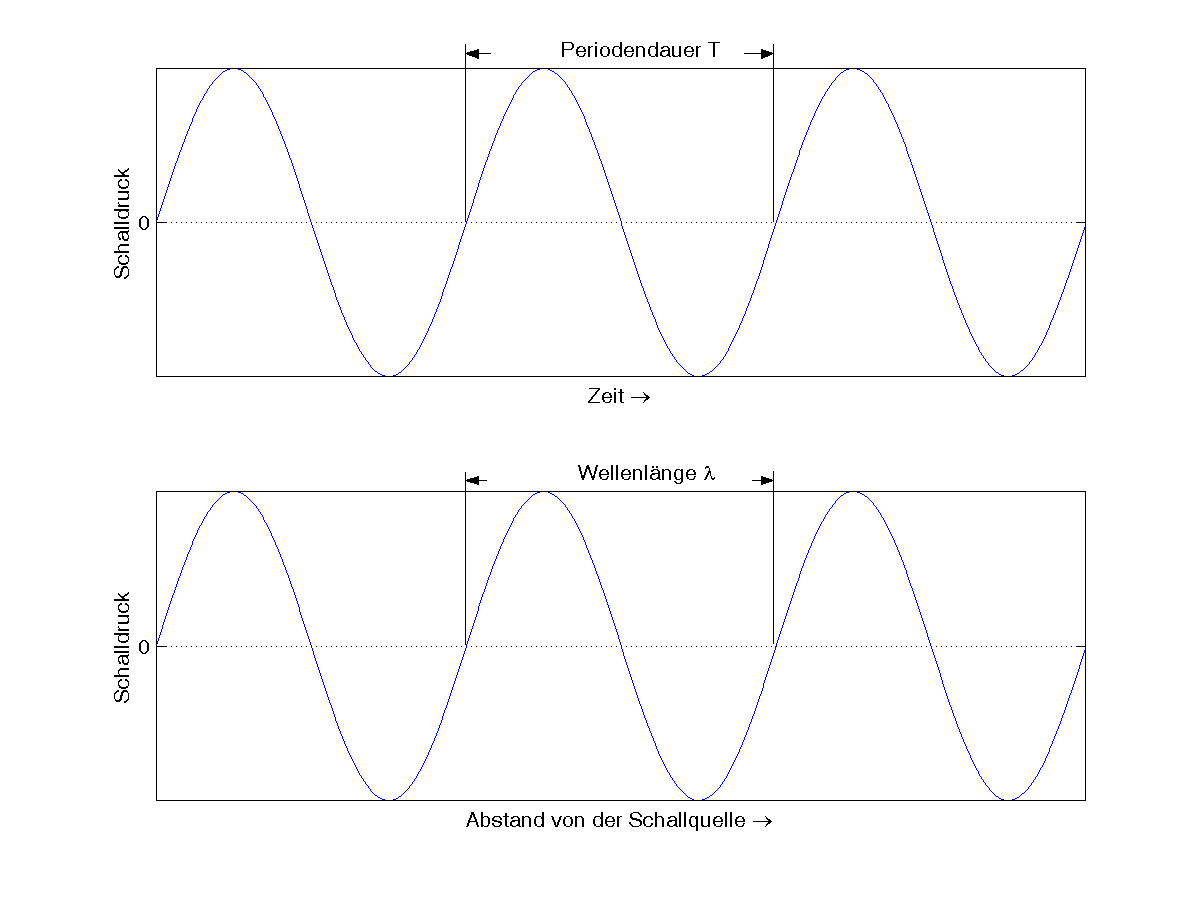
\includegraphics[scale=0.5]{Graph/msinus}
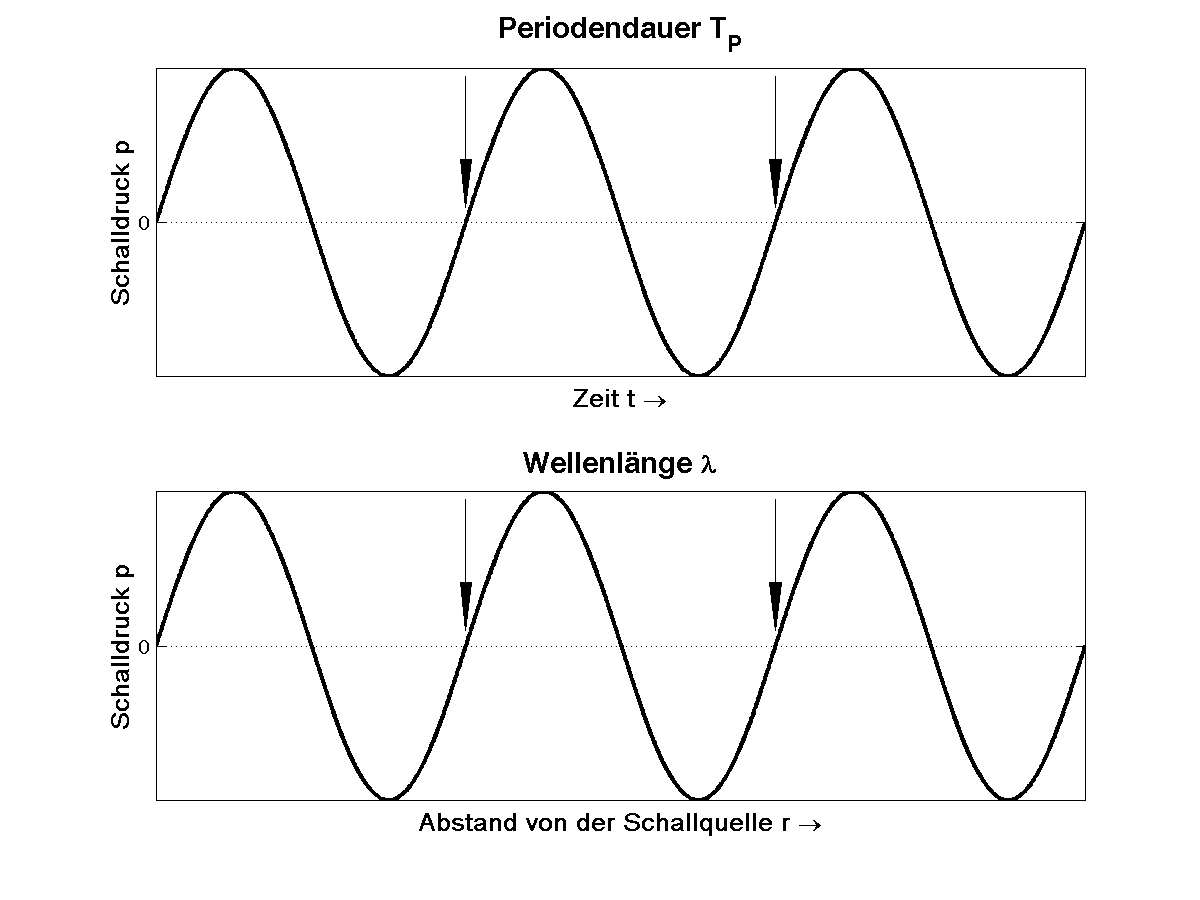
\includegraphics[scale=0.5]{Graph/n_schwingung}
\caption[Periodendauer und Wellenl�nge einer Schwingung]{Periodendauer und Wellenl�nge einer Schwingung}
\label{fig:sinus}
\end{center}
\end{figure}

Die in Abb. \ref{fig:sinus} dargestellte Schwingung ist in dieser Form erst einmal
nichtperiodisch, weil sie zeitlich begrenzt ist. Stellt man sich diese Schwingung aber auf
die gleiche Art und Weise rechts und links dieser Abbildung fortgesetzt vor, so erh�lt man
eine periodische Schwingung.
\end{sloppypar}
\bem{Sprache und Musik sind nichtperiodische Schwingungsvorg�nge. Man kann solche Signale
aber oft in kleine Abschnitte aufteilen, in denen die Schwingung periodisch erscheint; dann
spricht man von einer quasiperiodischen Schwingung. \\ Die nachfolgenden Gr��en beziehen
sich auf periodische Schwingungen. Ihr Bezug zu realen Signalen wie Sprache und Musik
beruht auf der Quasiperiodizit�t dieser Signale.}
\end{quote}
Die Punkte, an denen eine Sinusschwingung den Maximalausschlag, ihre Scheitelwerte,
erreicht, nennt man auch \textbf{Schwingungsbauch}\index{Schwingungsbauch|{bld}}. Nimmt sie
hingegen den Wert an, um den sie pendelt, so bezeichnet man diesen als
\textbf{Schwingungsknoten}\index{Schwingungsknoten|{bld}} (in Abb. \ref{fig:sinus} der Nulldurchgang).

\section{Frequenz und Periodendauer}\label{chap:freq}
Das Ma� f�r die H�ufigkeit, mit der sich eine periodische Schwingung wiederholt, ist die
\textbf{Frequenz}\index{Frequenz|{bld}} f. Sie gibt die Anzahl der Schwingungsperioden pro Sekunde an.

\begin{equation}\label{freq}
f=\frac{Anzahl\: der\: Schwingungen}{s}
\end{equation}

Die Einheit f�r die Frequenz ist somit die reziproke Sekunde $\left[\frac{1}{s}\right]$ bzw. Hertz [$H\!z$].
\\ Der
f�r Menschen h�rbare Frequenzbereich liegt in etwa zwischen $20H\!z$ und $20kH\!z$.
Schwingungen mit niedriger Frequenz klingen tief, Schwingungen h�herer Frequenz hoch.

\bem{Das Tonh�henempfinden ist \textit{nicht} dem Betrag einer Frequenz�nderung
proportional, sondern dem Verh�ltnis der �nderung. Zum Beispiel h�rt man bei einem Sprung
von $220H\!z$ auf $440H\!z$ eine Oktave, w�hrend man beim Sprung von $440H\!z$ auf $660H\!z$ eine Quinte
h�rt, obwohl beide Male $220H\!z$ zur unteren Frequenz addiert wurden. �ndert man aber die
Frequenz von $440H\!z$ auf $880H\!z$, so erklingt eine Oktave. Man h�rt also gleiche Intervalle,
wenn das Verh�ltnis $\frac{obere\: Frequenz}{untere\: Frequenz}$ gleich ist.}\end{quote}

Die Tabelle \ref{tab:freq_tonh} gibt Anhaltspunkte �ber den Frequenzumfang einzelner
Instrumente. Man erkennt, da� der h�rbare Frequenzbereich um einiges �ber die von diesen
Instrumenten erzeugten Grundschwingungen hinausgeht. Wir w�rden nur ein sehr dumpfes,
unvollst�ndiges Klangbild erleben, wenn wir beispielsweise nur bis $5kH\!z$ h�rten. Dies
h�ngt mit den von Instrumenten erzeugten Obert�nen zusammen, die ein wesentlich weiteres
Frequenzspektrum umfassen k�nnen (s. Abschnitt \ref{chap:ton_klang}).
\begin{table}[h]
\begin{center}
\begin{footnotesize}{\begin{tabular}{l|l|l}  \rule[-2mm]{0mm}{7mm}
\textbf{Frequenz} & \textbf{Note} & \textbf{Instrument} \\ \hline $16.5H\!z$ & $C_2$ & Taste
C im $32'$ der Orgel\\ \hline $33H\!z$ & $C_1$ & C-Saite bei f�nfseitigen Kontrab�ssen\\
\hline $66H\!z$ & $C$ & C-Saite der Violoncelli\\ \hline $131H\!z$ & $c$ & C-Saite der
Bratschen\\ \hline $262H\!z$ & $c'$ & tiefstes c der Geigen\\ \hline $524H\!z$ & $c''$ & hohes
c der Ten�re\\ \hline $1047H\!z$ & $c'''$ & hohes c der Soprane\\ \hline $2093H\!z$ & $c^4$ &
h�chstes c der Geigen\\ \hline $4185H\!z$ & $c^5$ & h�chstes c der Piccolo-Fl�ten\\ 
\end{tabular}}\end{footnotesize}\caption[Zuordnung von Frequenzwerten zu musikalischen
Tonbezeichnungen]{�berblick �ber die Zuordnung von Frequenzwerten zu musikalischen
Tonbezeichnungen (aus \cite{meyer})}
\end{center}\label{tab:freq_tonh}
\end{table}

Die Dauer einer Schwingungsperiode bezeichnet man als
\textbf{Periodendauer}\index{Periodendauer|{bld}} $T_{p}$. Sie ist der Kehrwert der Frequenz.

\begin{equation}\label{period}
T_{p}=\frac{1}{f}
\end{equation}
Die Einheit f�r die Periodendauer $T_{p}$ ist damit die Sekunde [s].

\bsp{Die Periodendauer der Schwingung einer Wasserwelle ist die Zeit, die ein Teilchen ben�tigt,
das immer auf und ab schwingt, um von einem Wellental ins n�chste zu gelangen.}
\end{quote}
\chaplink
\begin{itemize}
	\item Abschnitt \ref{chap:pitch}
\end{itemize}
\end{quote}


\section{Amplitude}\label{chap:amplitude}
Die \textbf{Amplitude}\index{Amplitude|{bld}} einer Schwingung ist der \glqq Scheitelwert\grqq$\:$
einer Schwingung, also ihr maximaler Ausschlag. Dieser Begriff wird haupts�chlich f�r
sinusf�rmige Schwingungen gebraucht.
Im Zusammenhang mit andersf�rmigen Schwingungen wird allerdings oft f�r f�r einen beliebigen Ausschlag der Begriff Amplitudenwert verwendet. Dies geschieht dann meistens zur Differenzierung z.B. zu Pegelwerten (s. Abschnitt \ref{chap:pegel}).
\chaplink
\begin{itemize}
	\item Abschnitt \ref{chap:lautstaerke}
	\ifthenelse{\equal{\value{allchaps}}{1}}
	{
		\item Abschnitt \ref{chap:fader}
	}{}
\end{itemize}
\end{quote}

\section{Phasenverschiebung}\label{chap:phaseshift}
Verschiebt man eine periodische Schwingung zu sich selber und vergleicht dann die
urspr�ngliche mit der verschobenen Schwingung, so sind diese beiden Schwingungen bis auf
die zeitliche Verschiebung $\Delta t$ immer noch identisch. F�r unterschiedliche Frequenzen
liegen die beiden gleichen Schwingungen bei konstanter Verschiebung immer unterschiedlich
zueinander. Aus diesem Grund gibt man die Verschiebung als Winkel an. Man setzt die
Periodendauer gleich $360$� und kann nun einen Winkel in Abh�ngigkeit von der zeitlichen
Verschiebung und der Frequenz bestimmen:
\begin{equation}\label{eq:phase}
\phi = \frac{\Delta t}{T_p}\cdot 360^\circ
\end{equation}
\begin{sloppypar}
Diesen Winkel nennt man dann \textbf{Phasenverschiebung}\index{Phasenverschiebung|{bld}} bzw.
\textbf{Phasendifferenz}\index{Phasendifferenz|{bld}} (s. Abb. \ref{fig:phase}), wenn man es ganz exakt ausdr�cken will
\textbf{Phasenwinkel}\index{Phasenwinkel|{bld}}. Dieser Wert ist abh�ngig von dem Verh�ltnis von Verschiebung und Periodendauer und
wird in der Praxis h�ufig verwendet.
\\ Um von einer Phasenverschiebung zu sprechen,
ben�tigt man immer einen Vergleichs- bzw. einen Bezugspunkt. Es ergibt keinen Sinn, eine
Schwingung phasenverschoben zu nennen, wenn keine zweite Schwingung angegeben wird, zu der
diese phasenverschoben ist. Es ist jedoch korrekt, von einer Phasendifferenz zwischen zwei
Schwingungen zu sprechen, oder diese beiden Schwingungen zueinander (um einen Winkel)
phasenverschoben zu nennen.
\end{sloppypar}
\bem{Das Ohr ist nicht in der Lage, die absolute Phasenverschiebung
einer Schwingung zu erkennen; es erkennt keinen Unterschied zwischen einer Schwingung und
der zeitlich verschobenen Schwingung. Treten allerdings die urspr�ngliche und die
verschobene Schwingung gleichzeitig auf, so l��t sich durchaus ein deutlicher Unterschied
wahrnehmen.}\end{quote}

\begin{figure}[!hbt]
\begin{center}
%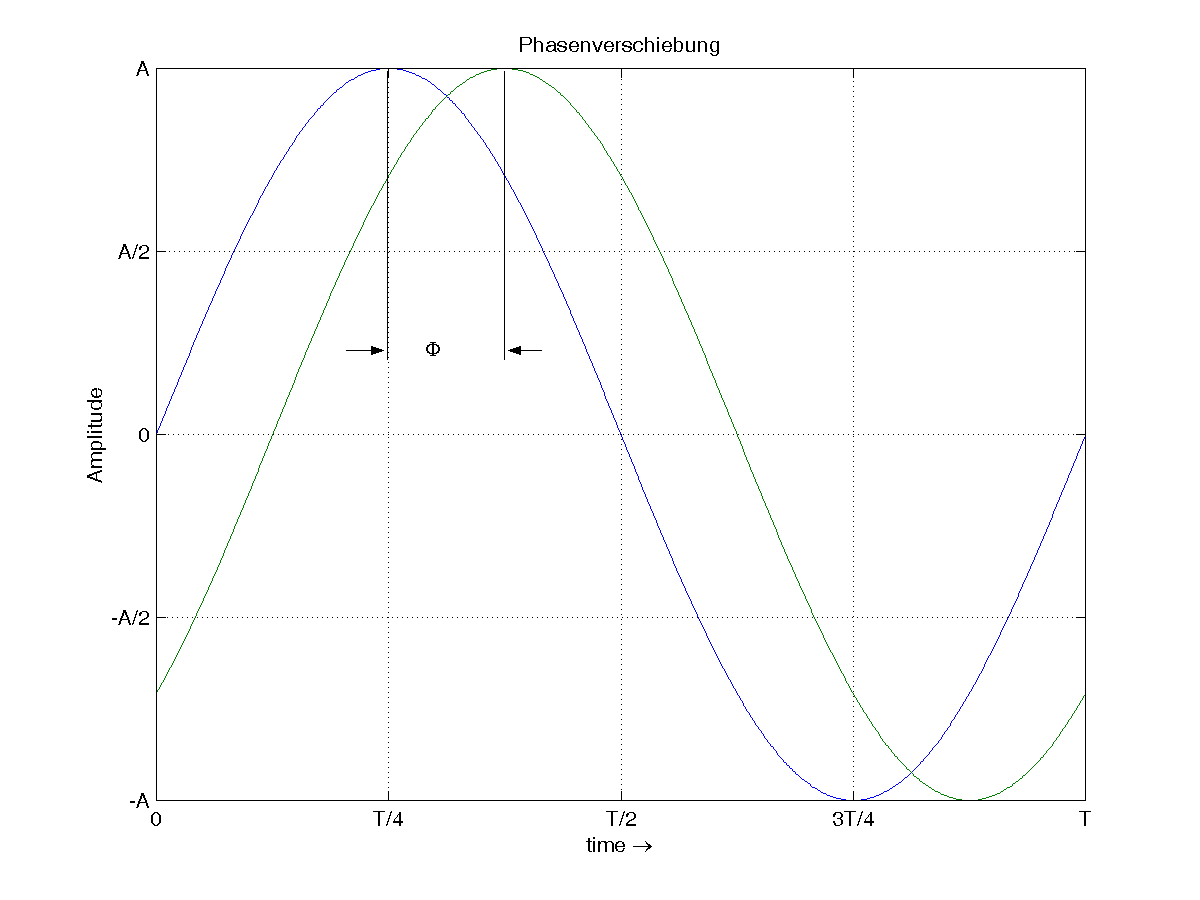
\includegraphics[scale=0.5]{Graph/mphase}
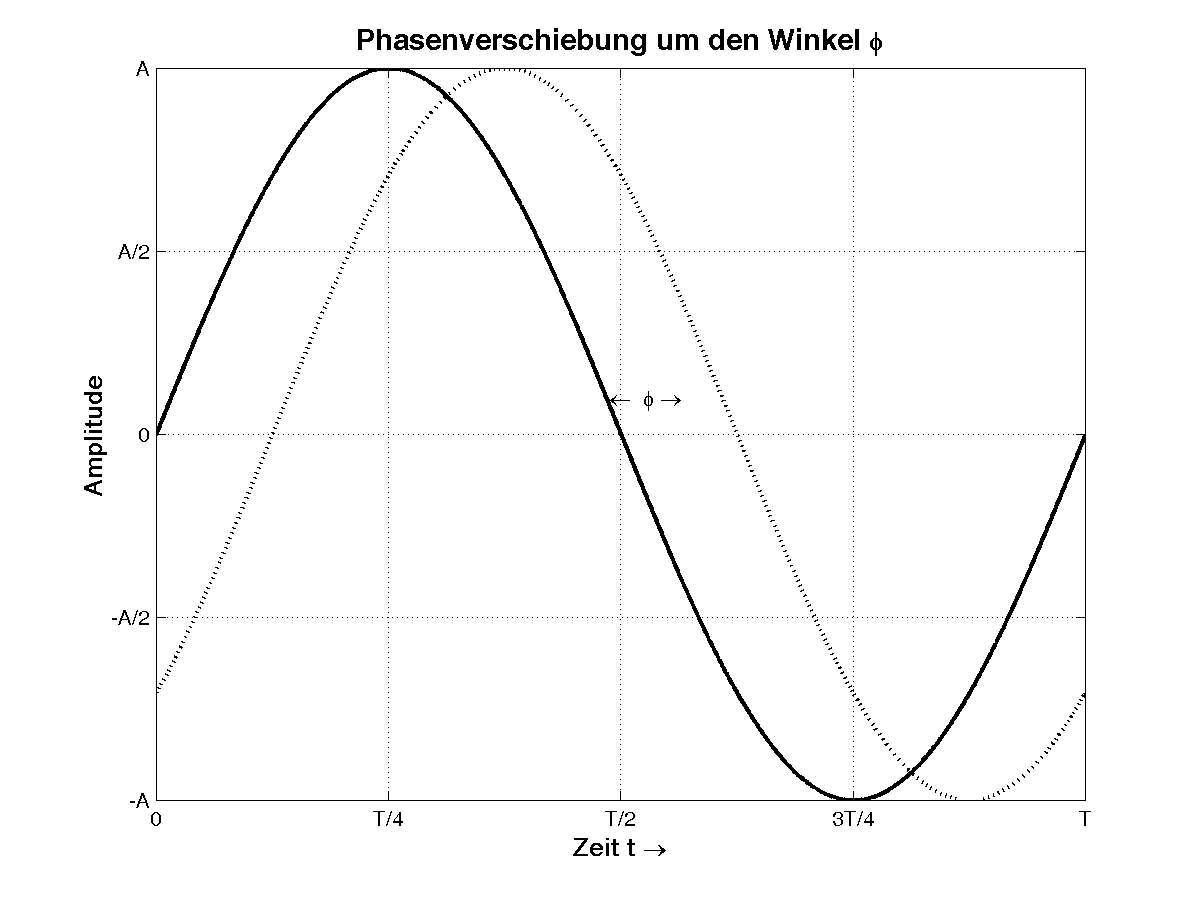
\includegraphics[scale=0.5]{Graph/n_phaseshift}
\caption[Phasenverschiebung um den Winkel $\phi$]{Phasenverschiebung um den Winkel $\phi$ bzw. um die Zeit $\Delta t$} \label{fig:phase}
\end{center}
\end{figure}

Werden zwei oder mehrere Schallwellen gleicher Frequenz �berlagert, so ergibt sich als
resultierendes Signal je nach Phasenwinkel ein entweder verst�rktes oder ged�mpftes Signal gleicher Frequenz. Ein weiterer Spezialfall ist die �berlagerung von sinusf�rmigen Schwingungen leicht unterschiedlicher Frequenz. Diese f�hrt zu einer sogenannten \bld{Schwebung}\index{Schwebung|{bld}} (vgl. Abb. \ref{fig:schwebung}) mit einer leicht verschobenen h�rbaren Frequenz und einer von der Differenzfrequenz abh�ngigen periodischen Amplituden�nderung. Eine solche Schwebung kann man leicht beim Stimmen eines Instrumentes h�ren; je n�her die beiden Frequenzen sind, desto langsamer wird die h�rbare Schwebung.
\begin{figure}[!hbt]
\begin{center}
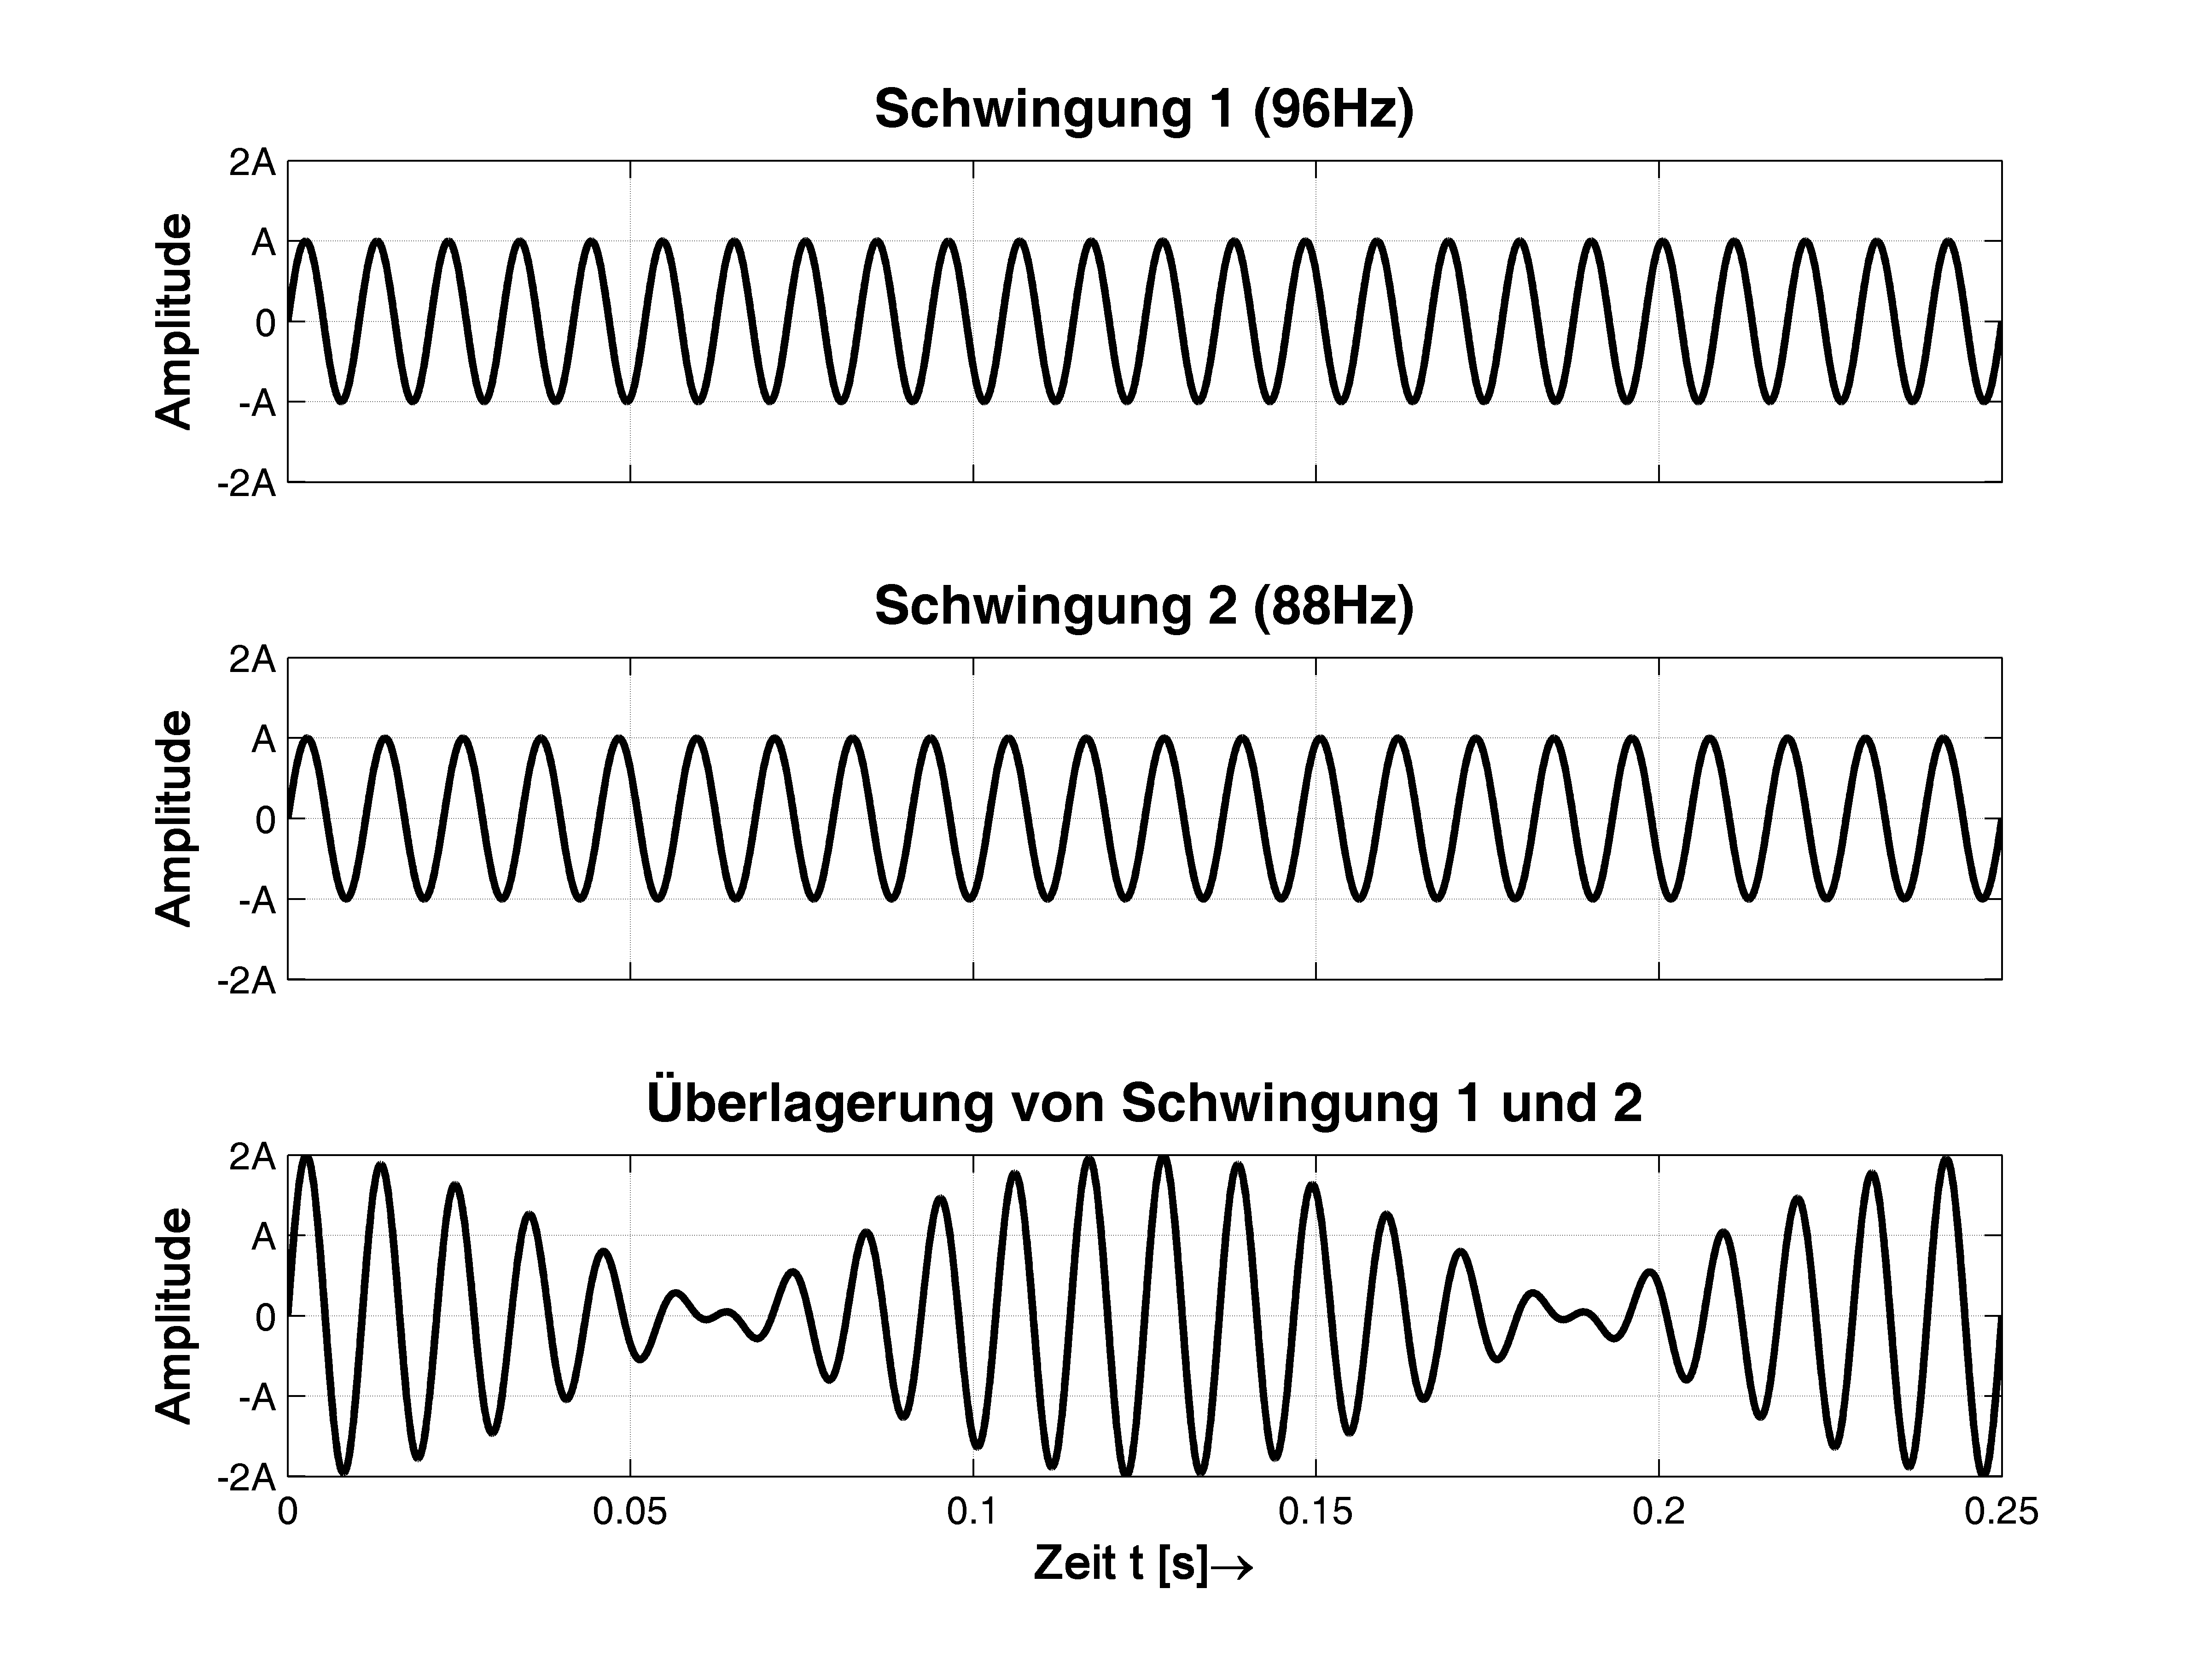
\includegraphics[scale=0.5]{Graph/n_schwebung}
\caption[Schwebung]{Schwebung aus der Addition (�berlagerung) zweier Schwingungen mit unterschiedlicher Frequenz} \label{fig:schwebung}
\end{center}
\end{figure}
\herl{Die Addition zweier sinusf�rmiger Schwingungen $y(t) = x_1(t) + x_2(t)$ mit leicht unterschiedlicher Frequenz l��t sich beschreiben durch:
\begin{equation}
	y(t) = \sin\left(2\pi f t\right) + \sin\left(2\pi \left(f-\Delta f\right) t\right)
\end{equation}
Nach den Additionstheoremen f�r trigonometrische Funktionen ergibt sich nun
\begin{eqnarray}
	y(t) &=& \sin\left(\frac{2\pi \left(f+f-\Delta f\right) t}{2}\right) \cdot \cos\left(\frac{2\pi \left[f-(f-\Delta f)\right] t}{2}\right)\\\nonumber
	&=& \sin\left(2\pi\frac{ f-\Delta f }{2}t\right) \cdot \cos\left(2\pi\frac{ \Delta f }{2}t\right)
\end{eqnarray}
}\end{quote}
Eine �berlagerung von Schwingungen wird \bld{Interferenz}\index{Interferenz|{bld}} genannt.\\

\chaplink
\begin{itemize}
	\item Abschnitt \ref{chap:leveladd}
\end{itemize}
\end{quote}

\section{T�ne, Kl�nge und Klangfarben}\label{chap:ton_klang}
Tonmeister bzw. Musiker verwenden die Begriffe \textit{Ton}\index{Ton|{bld}} und
\textit{Klang}\index{Klang|{bld}} anders als beispielsweise Akustiker. Um Verwirrungen vorzubeugen,
soll hier kurz auf die beiden Begriffe eingegangen werden.
\begin{figure}[!hbt]
\begin{center}
%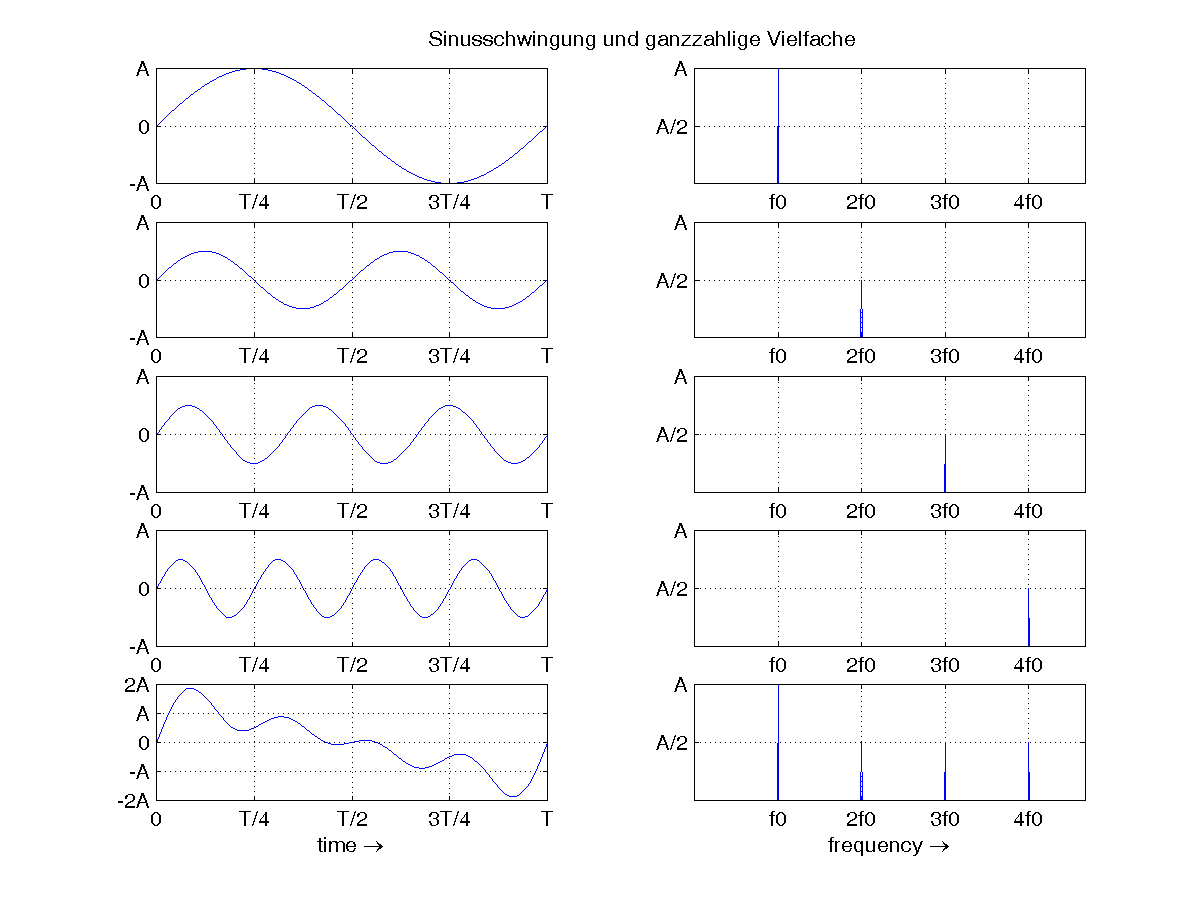
\includegraphics[scale=.7]{Graph/oberschwing}
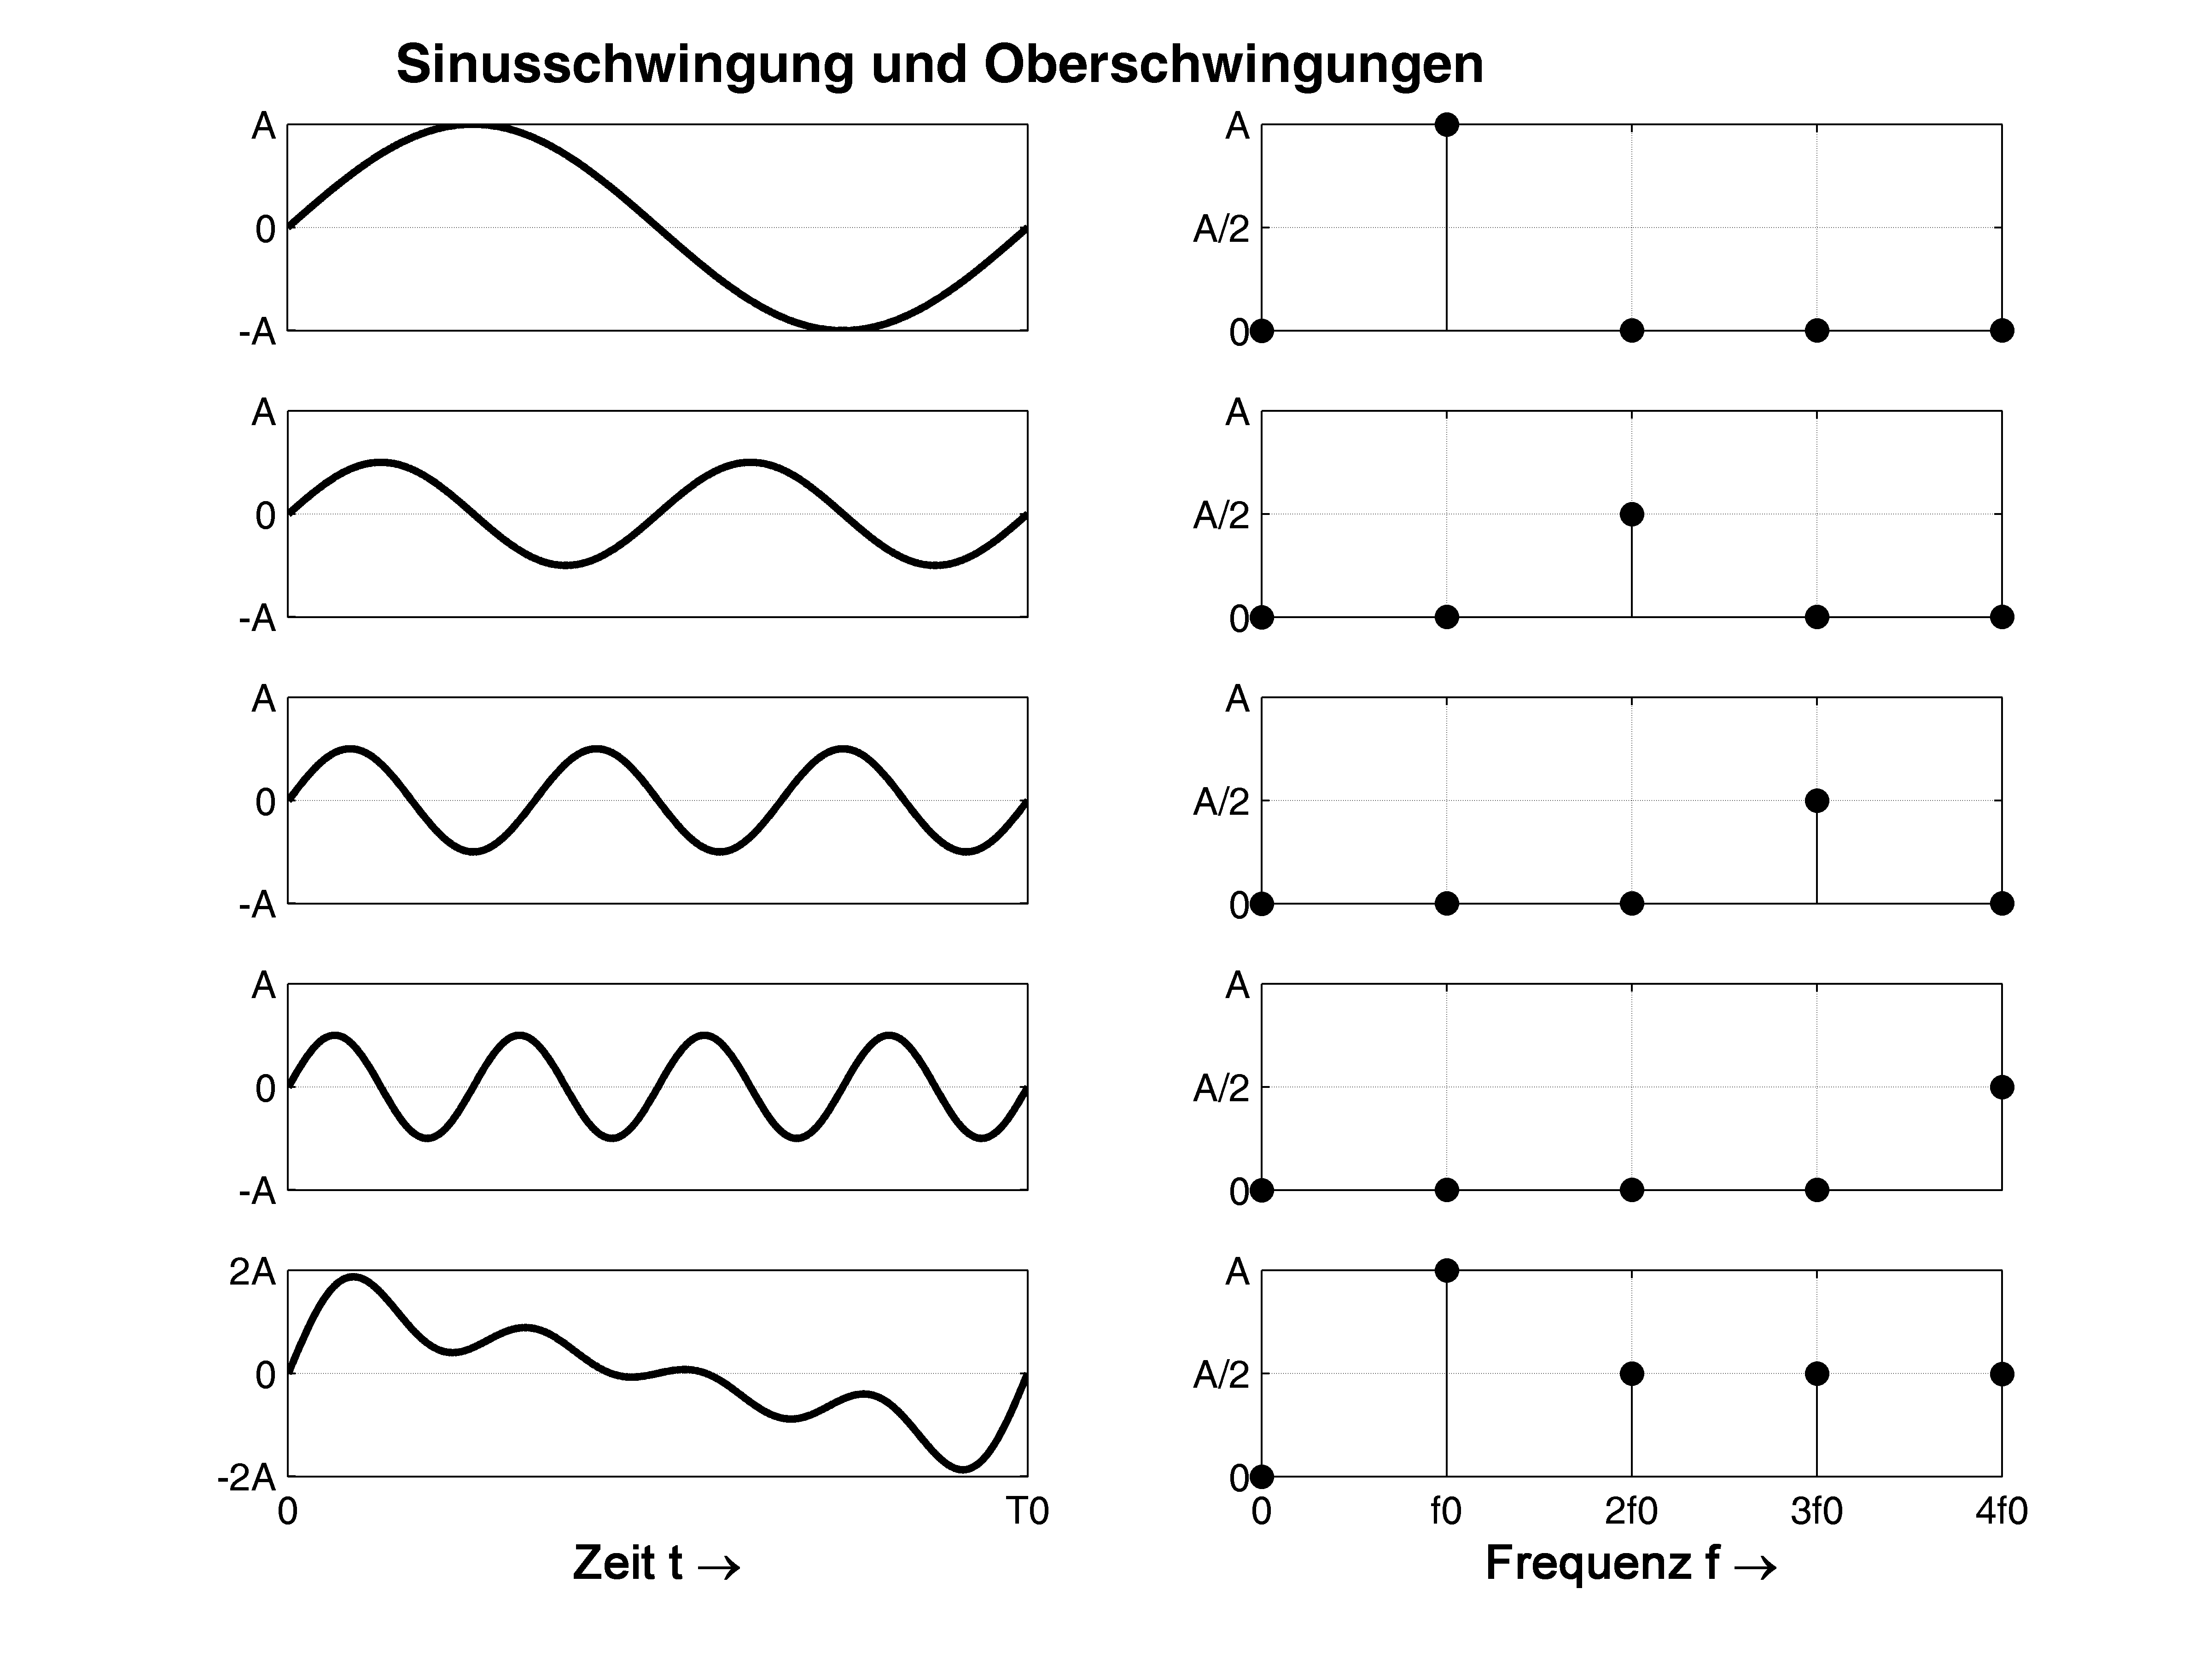
\includegraphics[scale=.5]{Graph/n_sineharm}
\caption[Sinusschwingung mit harmonischen Oberschwingungen]{Sinusschwingung und harmonische Oberschwingungen\index{Oberschwingung} im Zeitbereich (links) und im
Frequenzbereich (rechts). Die unterste Darstellung zeigt die Addition der Einzelschwingungen ebenfalls
im Zeit- und Frequenzbereich } \label{fig:schwingadd}
\end{center}
\end{figure}


Im wissenschaftlichen Gebrauch\footnote{nach DIN1320\cite{din1320}} ist eine Sinusschwingung einer
bestimmten Frequenz (im h�rbaren Bereich) ein Ton. Ein einzelner Ton in der Musik ist (je
nach Instrument) ein wesentlich komplexeres Gebilde, in jedem Fall aber ein Gemisch von
mehreren oder vielen verschiedenen Frequenzen. Akustiker w�rden ein solches Frequenzgemisch wiederum Klang
nennen. \\ 
Ein einzelner Ton eines beliebigen Musikinstrumentes zeichnet sich allgemein
durch sogenannte harmonische \textbf{Obert�ne}\index{Oberton|{bld}} aus, deren Frequenz ein
ganzzahliges Vielfaches der Grundfrequenz ist. Die Erh�hung der Frequenz jeweils um die Grundfrequenz f�hrt dabei zu immer kleineren Intervallen. Aus der Obertonreihe lassen sich daher die Frequenzverh�ltnisse der Intervalle (genauer der \glqq reinen\grqq$\;$ Intervalle) herleiten. Tabelle \ref{tab:intervals} zeigt die Frequenzverh�ltnisse f�r die ersten Intervalle.
\begin{table}[!htb]
\begin{footnotesize}
	\begin{center}
		\begin{tabular}{c|c}  \rule[-2mm]{0mm}{7mm}
                \bld{Frequenzverh�ltnis $f/f_0$} & \bld{reines Intervall}\\[1mm]\hline
					$1/1$			& Prime\\
					$2/1$			& Oktave\\
					$3/2$			& Quinte\\
					$4/3$			& Quarte\\
					$5/4$			& gr. Terz\\
					$6/5$			& kl. Terz\\
		\end{tabular}
 	\end{center}
\end{footnotesize}
			\caption[Frequenzverh�ltnisse reiner Intervalle]{Frequenzverh�ltnisse f�r reine Intervalle; die Frequenz einer reinen Quinte zur Grundfrequenz $f_0$ ist daher $\frac{3}{2}f_0$}
			\label{tab:intervals}
		\end{table}

\bem{Harmonische Obert�ne spielen beim H�ren eine sehr wichtige Rolle: aus der Struktur der harmonischen Obert�ne kann der H�rer
sogar selbst dann noch die Grundfrequenz h�ren, wenn diese physikalisch nur leise oder gar
nicht im Schallereignis vorhanden ist.}\end{quote}
\begin{figure}[!hbt]
\begin{center}
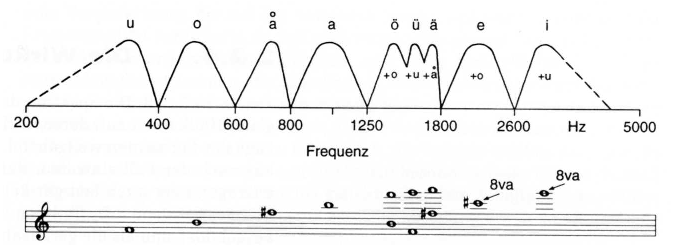
\includegraphics[scale=.85]{Graph/formant}
\caption[Frequenzlage der Formanten f�r die Vokale der deutschen Sprache]{Frequenzlage der Formanten f�r die Vokale der deutschen Sprache (aus \cite{meyer})}
\label{fig:formanten}
\end{center}
\end{figure}

Betrachtet man das Frequenzspektrum unterschiedlicher Instrumente, so erkennt man
(unabh�ngig von dem gerade gespielten Ton) instrumentenspezifische Frequenzbereiche, die
st�rker angehoben sind als andere und erheblichen Einflu� auf die Klangfarbe eines
Instrumentes haben. Solche Amplitudenmaxima innerhalb des Spektrums, deren Frequenz nicht
von der gespielten Tonh�he abh�ngt, nennt man \textbf{Formanten}\index{Formant|{bld}} oder
\textbf{Formantbereiche}\index{Formant!-bereich}. Die Klangfarben unterschiedlicher
Formanten lassen sich den Klangfarben von Vokalen zuordnen (s. Abb. \ref{fig:formanten}). So
klingen beispielsweise Instrumente mit einem starken Formanten
\textit{u} dunkel, w�hrend solche mit starkem Formanten \textit{i} hell und spitz klingen.

Neben der Frequenzstruktur des Klanges darf aber auch die klangliche Wirkung des Zeitverlaufs nicht untersch�tzt werden. Unterschiedliche Wirkungen verschiedener Musikinstrumente beruhen zu einem teilweise sehr hohen Ma�e auf der zeitlichen Struktur des Klanges. Einige wichtige Stichworte, die in sp�teren Abschnitten detaillierter erl�utert werden sind z.B. die H�llkurve\index{H�llkurve} und der Einschwingvorgang\index{Einschwingvorgang} eines Klangereignisses.

	\ifthenelse{\equal{\value{allchaps}}{1}}
	{
\chaplink
\begin{itemize}
	\item Abschnitt \ref{chap:timedesc}, \ref{chap:spectrumdesc}
	\item Abschnitt \ref{chap:filter}
	%\item Abschnitt \ref{chap:musak}
\end{itemize}
\end{quote}
	}{}

\section{Wellen}\label{chap:wellen}
Nachdem weiter oben schon das Wort \textbf{Welle}\index{Welle|{bld}} gefallen ist, mu� dieses
noch richtig definiert werden. Innerhalb eines Mediums (Wasser, Luft, Metall etc.) lassen
sich einzelne Molek�le zu Schwingungen anregen. Diese schwingenden Molek�le regen
ihrerseits auch die benachbarten Molek�le zu Schwingungen an, die ihre Bewegung wiederum an
die n�chsten Teilchen weitergeben. Diese Art der Ausbreitung ist eine Welle.

\section{Ausbreitungsgeschwindigkeit}
Die Geschwindigkeit, mit der sich eine Welle in Ausbreitungsrichtung fortpflanzt, nennt
sich \textbf{Ausbreitungsgeschwindigkeit}\index{Ausbreitungsgeschwindigkeit|{bld}} $c$. Wie jede
Geschwindigkeit hat diese die Einheit [$\frac{m}{s}$].
\bsp{Die Ausbreitungsgeschwindigkeit einer Wasserwelle ist die Geschwindigkeit, mit der
sich ein Wellenkamm in Ausbreitungsrichtung fortbewegt.}
\end{quote}

Die Ausbreitungsgeschwindigkeit ist abh�ngig von dem Medium, in dem sich die Welle
fortpflanzt. F�r Schallwellen wird sie als
\textbf{Schallgeschwindigkeit}\index{Schallgeschwindigkeit|{bld}} $c$ bezeichnet. In Luft ist die
Schallgeschwindigkeit abh�ngig von Temperatur, Luftfeuchtigkeit, Luftdruck und
Kohlendioxidgehalt. Sie ist \textit{nicht} abh�ngig von der Frequenz. W�hrend jedoch die
letztgenannten Gr��en (Luftfeuchtigkeit, Luftdruck und Kohlendioxidgehalt) zu
vernachl�ssigen sind, hat die Temperatur einen entscheidenden Einflu� (z.B. auf die
Stimmung von Instrumenten mit schwingender Lufts�ule wie Blasinstrumente oder Orgeln). Die
Schallgeschwindigkeit l��t sich abh�ngig von der Temperatur mit folgendem Ausdruck
berechnen:

\begin{equation}\label{eq:schallgeschw}
c=331.4\frac{m}{s}\cdot\sqrt{\frac{\zeta+273}{273}}
\end{equation}

\begin{quote}
\footnotesize{$\zeta$ ist die Temperatur in �C.}
\end{quote}

F�r die meisten �berschlagsrechnungen wird ein Wert von $c = 340 m/s$ angenommen.

\bem{F�r Zimmertemperatur ist der Wert $c = 340 m/s$ etwas niedrig angesetzt. Nach
Einsetzen in die Formel ergibt sich f�r eine Temperatur von 20�C $c = 343.3 m/s.$}
\end{quote}

\bem{Oft mu� eingesch�tzt werden, wie lange Schall braucht, um eine bestimmte Strecke
zur�ckzulegen. Da man nicht immer einen Taschenrechner parat hat, ist es sinnvoll, sich zu
merken, da� \textit{$1m$ ungef�hr in $3ms$ zur�ckgelegt wird}.}\end{quote}

\section{Wellenl�nge}
Bei der Ausbreitung einer periodischen Schwingung in einem Medium treten in bestimmten
Abst�nden in Ausbreitungsrichtung immer dieselben Schwingungszust�nde auf. Den Abstand
benachbarter gleicher Schwingungszust�nde bezeichnet man als \textbf{Wellenl�nge
$\lambda$}\index{Wellenl�nge|{bld}} mit der Einheit [m]. Die Wellenl�nge mu� somit von der
Frequenz f und der Ausbreitungsgeschwindigkeit, mit der sich eine Welle in einem Medium
fortpflanzt, abh�ngen. Man erh�lt

\begin{equation}\label{eq:lambda}
\lambda=\frac{c}{f}
\end{equation}

Die Wellenl�nge darf nicht mit der Periodendauer verwechselt werden; sie h�ngt zus�tzlich
noch von der Ausbreitungsgeschwindigkeit ab.
\bsp{Die Ausbreitungsgeschwindigkeit einer Wasserwelle ist die Geschwindigkeit, mit der
sich ein Wellenkamm in Ausbreitungsrichtung fortbewegt. Die Wellenl�nge einer solchen Welle
ist der Abstand zweier Wellenk�mme in Ausbreitungsrichtung.}
\end{quote}

\section{Ausbreitung von Wellen}
Bei der Form der Ausbreitung einer Welle kann man zwischen zwei Grenzf�llen unterscheiden,
der \textbf{Kugelwelle}\index{Welle!Kugel-|{bld}} und der \textbf{Ebenen
Welle}\index{Welle!ebene|{bld}}. Bei der Kugelwelle befinden sich alle Teilchen mit dem gleichen
Abstand zur Schallquelle im gleichen Schwingungszustand, bei der Ebenen Welle befinden sich
alle Teilchen auf einer Linie im gleichen Schwingungszustand. Von einer Ebenen Welle
spricht man auch, wenn man sich weit von einer Kugelschallquelle entfernt befindet, so da�
die Teilchen im gleichen Schwingungszustand sich n�herungsweise auf einer Linie befinden
(das gilt nat�rlich nur f�r einen begrenzten Ausschnitt aus der Kugel).


\bsp{Wasserwellen am Strand sind n�herungsweise Ebene Wellen, weil sich die gesamte
Wellenfront in einer Linie auf den Strand zu bewegt. Wenn man  in ruhiges Wasser einen
Stein wirft, dann breiten sich kreisrunde Wellen aus. Hier k�nnte man von einer Kugelwelle
sprechen.\\ 
Dieses Beispiel \glqq hinkt\grqq$\;$ insofern, als es sich auf zwei Dimensionen
beschr�nkt. �bertragen auf den Schall im Medium Luft mu� man das ganze auf drei Dimensionen
abstrahieren: aus Kreisen werden also Kugeln, die sich ausdehnen.}
\end{quote}

Die Wasserwelle, bei der sich ein bestimmtes Teilchen immer auf und ab bewegt, ist
sicherlich ein anschauliches Beispiel einer Welle. Man sollte dieses Beispiel aber nicht
�berstrapazieren, da einige Eigenschaften der Wasserwellen nicht mit denen von Schallwellen
�bereinstimmen. Vor allem schwingen die Teilchen in der Luft nicht auf und ab, sondern in
Ausbreitungsrichtung des Schalls, d.h. wenn der Schall sich beispielsweise nach rechts
ausbreitet, so schwingen die Teilchen auch von rechts nach links und nicht von oben nach
unten. Eine solche Welle, bei der die Teilchen in Ausbreitungsrichtung schwingen, wird
allgemein \textit{longitudinale Welle} genannt.

\section{Zusammenfassung}
Eine Welle besteht aus Schwingungen einzelner Teilchen. Eine Schwingung wird gekennzeichnet
durch die \textbf{Frequenz} $f$, welche die Anzahl an Schwingungen pro Sekunde angibt, bzw.
die \textbf{Periodendauer} $T_{p}$, den Kehrwert von $f$ und die Amplitude ihrer einzelnen
Schwingungszust�nde. Bei gegeneinander verschobenen Schwingungen kann man die
\textbf{Phasendifferenz} bzw. den \textbf{Phasenwinkel} angeben. Eine Welle kann
prinzipiell beschrieben werden durch die \textbf{Wellenl�nge $\lambda$} und die
\textbf{Ausbreitungsgeschwindigkeit}. Die Ausbreitungsgeschwindigkeit h�ngt vom Medium und
seinen Eigenschaften ab, bei Luft insbesondere auch von der Temperatur. Die
Ausbreitungsgeschwindigkeit von Schall hei�t \textbf{Schallgeschwindigkeit} $c$. Bei der
Ausbreitungsart einer (Schall-)Welle wird zwischen den beiden Grenzf�llen
\textbf{Kugelwelle} und \textbf{Ebene Welle} unterschieden.

\section{Aufgaben}
\begin{enumerate}
 \item  In welcher Zeit legt Schall bei normaler Zimmertemperatur eine Strecke von $10 m$
 zur�ck?
 \item  Eine periodische Schwingung wird mit der gleichen um $180^\circ$ verschobenen
 Schwingung addiert. Wie sieht das Ergebnis aus?
 \item  Was ist der Unterschied zwischen Periodendauer $T_{p}$ und Wellenl�nge $\lambda$?
 \item  Berechne die Wellenl�ngen $\lambda$ f�r folgende Frequenzen bei $c = 340 m/s$.
   \begin{itemize}
   \item	$16H\!z$
   \item	$100H\!z$
   \item	$1000H\!z$
   \item	$10000H\!z$
   \item	$20000H\!z$
   \end{itemize}
 \item  Berechne die Frequenz des Tones a` f�r die angegebenen Temperaturen, wenn sie bei $14.35 ^\circ C$ $440H\!z$ betr�gt und die Wellenl�nge konstant bleibt.
   \begin{itemize}
   \item	$16^\circ C$
   \item	$19^\circ C$
   \item	$22^\circ C$
   \end{itemize}
 \item  Ist der oben berechnete Tonh�henunterschied gravierend oder ver\-nach\-l�ssig\-bar?
\end{enumerate}
% m�gliche Ger�te: Sinusgenerator
	\chapter{Schall und Schallfeld}\label{chap:schall}
\thispagestyle{empty}

Nachdem im vorigen Kapitel die Begriffe Schwingung und Welle erl�utert wurden, wird dieses Kapitel die wichtigen Gr��en f�r Schall einf�hren, und auf die Besonderheiten der Schallausbreitung eingehen. 

\section{Schallschnelle und Schalldruck}
\thispagestyle{empty}
Wie bereits in Abschnitt \ref{chap:wellen} beschrieben, breitet sich eine Schallwelle mittels
Hin- und Herbewegung von Luftteilchen in Ausbreitungsrichtung aus. Die Geschwindigkeit, mit
der die Teilchen sich bewegen, hat mit der Schallgeschwindigkeit $c$, mit der sich eine
Welle fortpflanzt, \textit{nichts} zu tun. Die Geschwindigkeit, mit der einzelne Teilchen
um den Ort pendeln, an dem sie sich in Ruhe bef�nden, wird
\textbf{Schallschnelle v}\index{Schallschnelle|{bld}} genannt.

\bsp{ Die Schallschnelle eines Teilchens ist \textit{keine} konstante Gr��e. Sie ist an dem
urspr�nglichen Ruhepunkt des Teilchens am gr��ten und bei der maximalen Auslenkung gleich
Null. Zur Veranschaulichung kann man sich ein schwingendes Teilchen also wie ein
schwingendes Pendel vorstellen. Das bedeutet auch, da� die Luftteilchen nicht mit der Welle
mitwandern.}\end{quote}

Die Luftteilchen schwingen in Ausbreitungsrichtung und regen ihrerseits Nachbarteilchen zum
Schwingen an. Somit folgt eine Schwankung der Dichte und damit �nderungen des Drucks. Diese
Druck�nderungen bezeichnet man als
\textbf{Schalldruck}\index{Schalldruck|{bld}} $p$. Der Schalldruck wird vom Ohr wahrgenommen; das
Ohr ist ein Schalldruckempf�nger.
\begin{figure}[!hbt]
\begin{center}
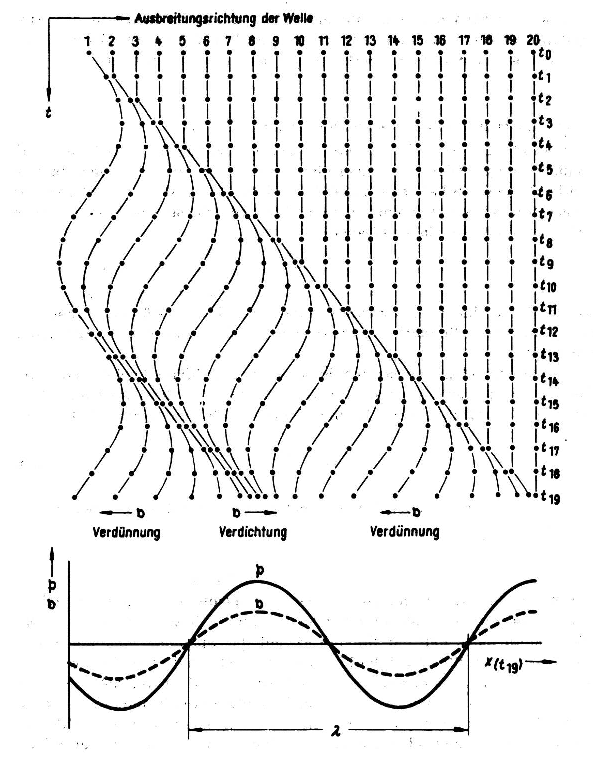
\includegraphics{Graph/ausbrtg}
\end{center}
\caption[Ausbreitung einer Welle und Schalldruck]{Ausbreitung einer Welle und Schalldruck (aus \cite{webers})\label{fig:longitud}}
\end{figure}
Der Schalldruck hat einen Wert f�r einen bestimmten Punkt im Raum, die Schallschnelle
hingegen hat zudem noch eine Richtung, weswegen man sie als Vektor schreibt.

\begin{sloppypar}
Schallschnelle und Schalldruck sind Wechselgr��en, d.h. sie �ndern sich st�ndig. Man m�chte
sie aber gerne durch jeweils einen einzelnen Wert ausdr�cken. Hierf�r hat sich der
sogenannte \bld{Effektivwert}\index{Effektivwert|{bld}}(englisch: RMS f�r Root Mean Square) eingeb�rgert. Streng ist dieser
definiert durch\end{sloppypar}
\begin{equation}\label{eq:effektivp}
  p_{eff}=\sqrt{\lim_{T \rightarrow \infty} \frac{1}{T}\int_{T}\left[p(t)\right]^2 \,dt}\; \left[Pa\right],
\end{equation}
f�r einfache periodische Signale (mit der Periodendauer T) kann man ihn aber auch durch
\begin{equation}\label{eq:effektivp2}
  p_{eff}=\sqrt{\frac{1}{T}\int_{T}\left[p(t)\right]^2 \,dt}\;\left[Pa\right]
\end{equation}
berechnen. Ebenso l��t sich der Effektivwert der Schallschnelle ermitteln.
\bem{Man meint,
wenn von Schalldruck oder Schallschnelle als absoluten Gr��en die Rede ist, fast immer den
Effektivwert (auch wenn das nicht explizit erw�hnt wird), denn auf diese Weise lassen sich
diese Wechselgr��en als einzelne Werte behandeln.}
\end{quote}
\bem{Gegen�ber dem statischen Luftdruck ist der Schalldruck au�erordentlich klein. Der
atmosph�rische Druck betr�gt $10^5Pa$ \footnote{$1Pa=1\frac{N}{m^2}$}, w�hrend der
Schalldruck bei mittlerer Lautst�rke ca. $1/10Pa$ betr�gt. Der maximal ertr�gliche
Schalldruck, die Schmerzschwelle, liegt bei ca. $100Pa$.}
\end{quote}

\section{Entfernungsabh�ngigkeit des Schalldrucks}
\begin{sloppypar}
Der Schalldruck nimmt mit zunehmender Entfernung ab, eine weit entfernte Schallquelle wird
wesentlich leiser wahrgenommen als eine nahe (wenn beide gleichstark abstrahlen). Es l��t
sich zeigen, da� der Schalldruck umgekehrt proportional zur Entfernung $r$
ist\footnote{Dies gilt f�r Kugelschallquellen. F�r andere Schallquellen nimmt der
Schalldruck bis zu einer bestimmten Entfernung langsamer ab, und verh�lt sich dann wie im
Kugelschallfeld.}, d.h.
\begin{equation}\label{eq:r-gesetz}
  p\sim \frac{1}{r}.
\end{equation}

Das bedeutet also, \textit{da� sich bei jeder Entfernungsverdopplung der Schalldruck
halbiert}. Diese Gesetzm��igkeit nennt man oft \textbf{1/r-Gesetz}\index{Gesetz!1/r-|{bld}}. Sie
folgt direkt als L�sung der sogenannten Wellengleichung, die man f�r eine Kugelschallquelle
aufstellen kann.
\end{sloppypar}
\bem{Prinzipiell gilt dieses Gesetz genau wie die im folgenden Abschnitt \ref{chap:nahfern} erl�uterte Abh�ngigkeit der
Schallschnelle von der Entfernung nur im sogenannten Freifeld (s. Abschnitt
\ref{chap:freifeld}), d.h. nicht in normalen R�umen, sondern nur im Freien oder im
reflexionsarmen Raum. N�herungsweise kann man aber auch in normalen R�umen von dieser
Gesetzm��igkeit ausgehen, allerdings nur in N�he der Schallquelle (s. Abschnitt
\ref{chap:freifeld}. }\end{quote}

\section{Nahfeld und Fernfeld/ Entfernungs\-ab\-h�n\-gig\-keit der Schallschnelle}\label{chap:nahfern} Als L�sung der Wellengleichung f�r die Schallschnelle
ergibt sich eine etwas komplexere Beziehung als f�r den Schalldruck. Ist man weit von der
Schallquelle entfernt, so nimmt der Betrag der Schallschnelle genauso wie beim Schalldruck
mit $1/r$ ab. Nahe an der Schallquelle nimmt die Schnelle aber nicht nur mit $1/r$, sondern
mit $1/r^2$ ab. Man unterscheidet je nach Verhalten der Schnelle zwischen
\textbf{Nahfeld}\index{Nahfeld|{bld}} ($1/r^2-Abnahme$) und \textbf{Fernfeld}\index{Fernfeld|{bld}} (Abnahme mit $1/r$).

\herl{Man erh�lt als L�sung der Wellengleichung f�r den Betrag der Schnelle
\begin{equation}\label{eq:schnellebetrag}
  |\mathbf{v}|\sim \frac{1}{r}\sqrt{1+\left(\frac{\lambda}{2\pi r}\right)^2}
\end{equation}
\begin{quote}
\scriptsize{$r$ ist der Abstand zur Kugelschallquelle,\\ $\lambda$ ist die Wellenl�nge des
abgestrahlten Schalls}
\end{quote}
Der Betrag der Schallschnelle ist also sowohl von der Entfernung, als auch von der
abgestrahlten Wellenl�nge abh�ngig. Man erkennt, wenn man f�r $r$ gro�e Werte einsetzt, da�
die Summe unter der Wurzel sehr nahe bei $1$ liegt. Dies bedeutet, da� man f�r gro�e Werte
von $r$ (d.h. gro�e Abst�nde von der Schallquelle) die Beziehung
\begin{equation}\label{eq:schnellefern}
   |\mathbf{v}|\sim \frac{1}{r}\sqrt{1}
\end{equation}
erh�lt, also die gleiche Abnahme wie beim Schalldruck. Setzt man f�r $r$ allerdings sehr
kleine Werte ein, so kann man die $1$ der Summe unter der Wurzel vernachl�ssigen und erh�lt
\begin{equation}\label{eq:schnellenah}
   |\mathbf{v}|\sim \frac{1}{r^2}.
\end{equation}
Den �bergang zwischen Nahfeld und Fernfeld findet man, wenn der zweite Summand
${\frac{\lambda}{2\pi r}}^2$ die gleiche Gr��enordnung hat wie der erste Summand, also
ungef�hr bei $\frac{\lambda}{2\pi r}=1$. Der Punkt des �bergangs ist also frequenzabh�ngig,
oder anders ausgedr�ckt: die Ausdehnung des Nahfeldes ist abh�ngig von der abgestrahlten
Wellenl�nge.}
\end{quote}

\begin{figure}[!hbt]
\begin{center}
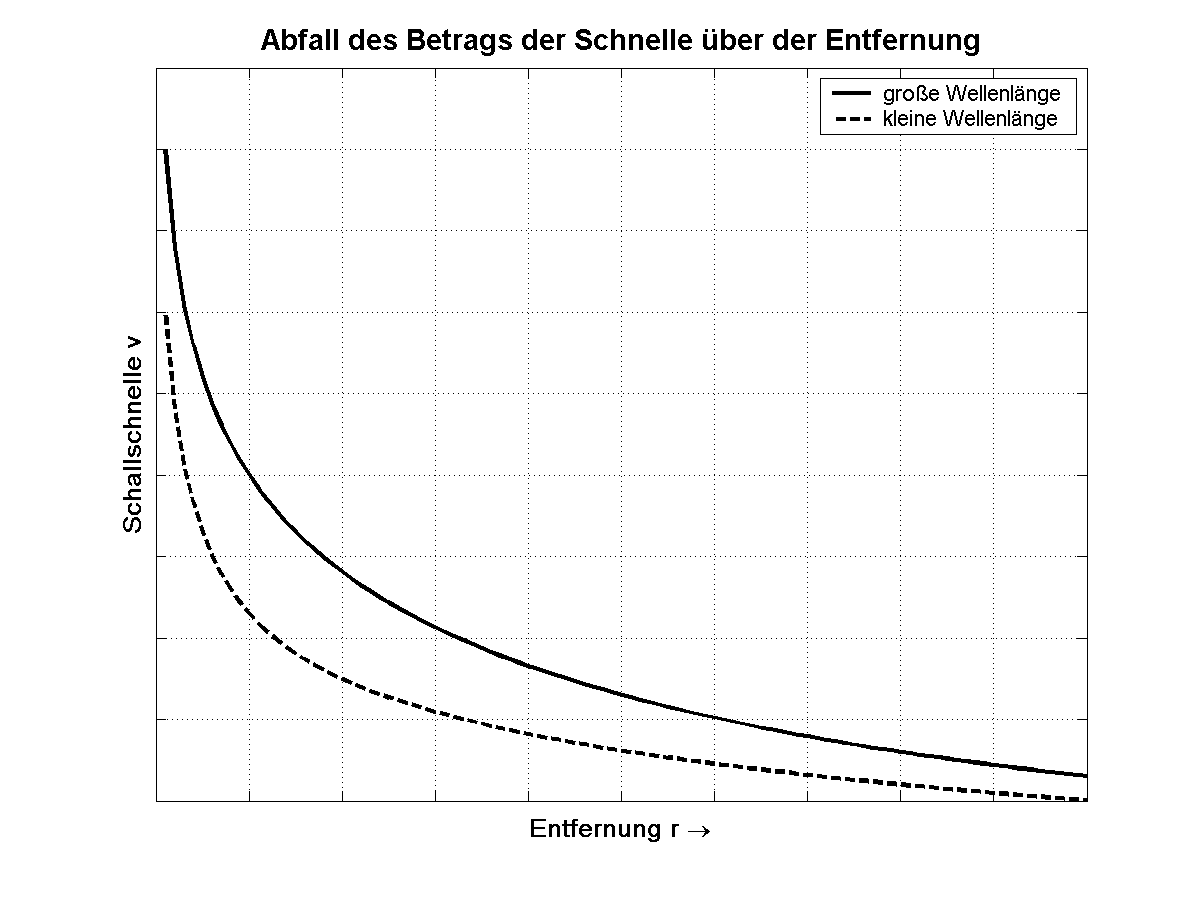
\includegraphics[scale=0.5]{Graph/n_nahfeld}
\caption[Verlauf der Schallschnelle �ber dem Abstand $r$]{Verlauf der Schallschnelle �ber dem Abstand $r$ von der Schallquelle f�r zwei
verschiedene Frequenzen} \label{fig:nahfern}
\end{center}
\end{figure}

Bei tiefen Frequenzen mu� man wesentlich weiter von der Schallquelle entfernt sein, um sich
im Fernfeld zu befinden, als f�r h�here. Den �bergang von Nah- zu Fernfeld findet man, wie
in der Herleitung erw�hnt, im Abstand
\begin{equation}\label{eq:nahzufern}
  r=\frac{\lambda}{2\pi}.
\end{equation}
Ein weiterer Unterschied zwischen Nah- und Fernfeld ist von Bedeutung. Im Fernfeld befinden
sich Schalldruck und Schallschnelle in Phase, w�hrend sie im Nahfeld um bis zu 90�
zueinander phasenverschoben sind.

\bem{F�r Mikrophone, die keine reinen Schalldruckempf�nger sind, sondern auf die
Schallschnelle ansprechen, ist das Wissen um Nah- und Fernfeld einer Schallquelle von
Bedeutung. Schnelleempf�nger liefern einerseits eine um 90� zu Druckempf�ngern verschobene
Ausgangsspannung, andererseits erh�lt man bei solchen Mikrophonen im Nahfeld eine sehr
starke Anhebung der tiefen Frequenzen. Dies wird
\emp{Nahbesprechungseffekt}\index{Nahbesprechungseffekt} genannt. Dazu in Abschnitt ?????? mehr.
}\end{quote}

\section{Schalleistung}
Die St�rke des Schalldrucks an einem bestimmten Punkt im Raum ist durch die \glqq
St�rke\grqq$\:$  der Schallquelle bestimmt. Es ist von Interesse, die St�rke einer Schallquelle
unabh�ngig vom Abstand des H�rers und den r�umlichen Gegebenheiten angeben zu k�nnen. Die
\textbf{Schalleistung $P_{ak}$}\index{Schalleistung|{bld}}, also die abgestrahlte Energie pro
Sekunde, ist eine Gr��e, die dies erm�glicht. Ihre Einheit ist Watt [W]. Sie ist
\begin{equation}\label{eq:schalleistung}
  P=p_{eff}^2= \lim_{T \rightarrow \infty}\frac{1}{T}\int_{T}{\left[p(t)\right]^2 \,dt}\;[W].
\end{equation}


\section{Schallintensit�t}
Die \textbf{Schallintensit�t}\index{Schallintensit�t|{bld}} ist die Schalleistung, die durch eine
senkrecht zur Ausbreitungsrichtung stehende Fl�che str�mt.
\begin{equation}\label{eq:intensitaet}
  \mathbf{J}=\frac{1}{T}\int_0^T{p(t)\cdot \mathbf{v}(t)\,dt}\;\left[\frac{W}{m^2}\right]
\end{equation}
F�r eine Kugelschallquelle gilt f�r
die Intensit�t in Abh�ngigkeit des
\mbox{Abstandes $r$}
\begin{equation}\label{eq:intensikugel}
  J(r)=\frac{P_{ak}}{4\pi r^2}\;\left[\frac{W}{m^2}\right]
\end{equation}

\section{Gest�rte Schallausbreitung}
In den vorigen Abschnitten wurde davon ausgegangen, da� die Schallwelle sich ungest�rt
ausbreiten kann, also auf keine Hindernisse st��t. In R�umen gibt es eine Vielzahl von
Hindernissen, die den Schall an ungest�rter Ausbreitung hindern, insbesondere nat�rlich die
W�nde. Je nach Art und Beschaffenheit des Hindernisses entstehen verschiedene Ph�nomene. Im
folgenden soll kurz auf diese eingegangen werden.

\subsection{Reflexion}
Trifft eine Schallwelle auf eine ebene Fl�che, die gro� im Verh�ltnis zu ihrer Wellenl�nge
ist, so wird sie reflektiert. Hierf�r gilt - genau wie in der Optik - das bekannte Gesetz
Einfallswinkel = Ausfallswinkel, das besagt, da� die unter einem Winkel $\theta$ (die
$0^\circ $-Achse steht senkrecht auf der Wand) auf die Wand treffende Welle mit einem Winkel
$-\theta$ wieder reflektiert wird. Schall verh�lt sich hier also wie ein Strahl (s.
Abb. \ref{fig:reflex}).

\begin{figure}[!hbt]
\begin{center}
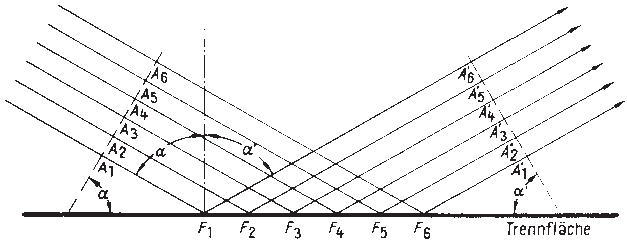
\includegraphics{Graph/reflex2}
\caption[Reflexion einer Ebenen Welle]{Reflexion einer Ebenen Welle mit Einfallswinkel $\alpha$ an einer Wand (aus \cite{webers})} \label{fig:reflex}
\end{center}
\end{figure}
\begin{sloppypar}
Je nach Material der Wand sind die Reflexionen allerdings nicht mehr mit dem eintreffenden
Schall identisch. Vielmehr reflektieren verschiedene Wandmaterialien verschiedene
Frequenzen unterschiedlich gut. Beispielsweise reflektiert eine harte Steinwand den
eintreffenden Schall fast verlustlos, w�hrend eine mit Stoff bespannte Wand hohe Frequenzen
d�mpfen wird.\\
\end{sloppypar}
Die Eigenschaft eines (Wand-)materials, nicht die gesamte Schallenergie zu reflektieren,
sondern nur einen Teil, kann mit dem \textbf{Absorptionsgrad}\index{Absorptionsgrad|{bld}}
$\alpha$ beschrieben werden. Der Absorptionsgrad eines Materials, das keinen Schall
reflektiert, sondern alles absorbiert, ist $\alpha=1$; f�r eine verlustfrei reflektierende
Wand w�re $\alpha=0$. F�r reale Materialien kann der Absorptionsgrad also Werte zwischen
$0$ und $1$ annehmen.


\bem{Bei verlustbehafteter Reflexion (s.o.) spricht man von \textit{Schalld�mpfung}\index{Schalld�mpfung|{bld}}. Wenn
man sich dagegen beispielsweise nicht im gleichen Raum wie das Schallereignis aufh�lt,
sondern im Nebenraum, so erreicht den H�rer nur die Schallenergie, die weder reflektiert
noch absorbiert, sondern durchgelassen wurde. Diese Eigenschaft einer Wand bezeichnet man
als \textit{Schalld�mmung}\index{Schalld�mmung|{bld}}}
\end{quote}

\chaplink
\begin{itemize}
	\item Abschnitt \ref{chap:raumak}
\end{itemize}
\end{quote}

\subsection{Beugung}\label{chap:beugung}
Bei der Reflexion von Schall war die Voraussetzung, da� die reflektierende Fl�che gro�
gegen�ber der Wellenl�nge ist. Ist die Wellenl�nge hingegen in der gleichen Gr��enordnung
wie die Fl�che (resp. ihre kleinste Ausdehnung), so werden die Schallwellen nicht mehr
reflektiert, sondern gebeugt.
\textbf{Beugung}\index{Beugung|{bld}} bedeutet, da� die Schallwellen sich um das Hindernis \glqq
herumbiegen\grqq. Ist das Hindernis also klein gegen�ber der Wellenl�nge, so treten also
dahinter kaum Abschattungswirkungen auf, sondern die Schallwelle pflanzt sich hinter dem
Hindernis fast genau wie vor dem Hindernis fort (s. Abb. \ref{fig:beugung}).
\begin{figure}[!hbt]
\begin{center}
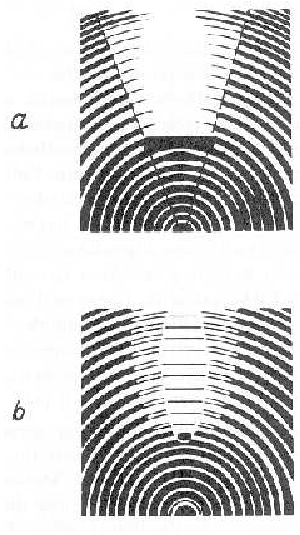
\includegraphics{Graph/beugung}
\caption[Beugung von Wellen hinter einem Hindernis]{Beugung von Wellen hinter einem Hindernis: (a) Hindernis gro� im Vergleich zu der
Wellenl�nge, (b) Hindernis gleich gro� wie die Wellenl�nge (aus \cite{webers})}
\label{fig:beugung}
\end{center}
\end{figure}

\section{Zusammenfassung}\begin{sloppypar}
Schall breitet sich als \textit{longitudinale Welle} aus. Die Luftteilchen schwingen um
ihren Ruhepunkt mit der \textbf{Schallschnelle \textit{v}} und erzeugen durch ihre Bewegung
Druckschwankungen, den \textbf{Schalldruck \textit{p}}. Beide Gr��en sind Wechselgr��en und werden
zumeist nur mit ihrem \textit{Effektivwert} angegeben. Seltener werden in der
Tonstudiotechnik f�r Berechnungen oder Angaben auch die \textbf{Schalleistung}
$P_{ak}$ oder die
\textbf{Schallintensit�t \textit{J}} verwendet.\\ Der Schalldruck nimmt bei Entfernung von der
Schallquellen mit $1/r$ ab, dies besagt das sogenannte \textbf{$1/r$-Gesetz}. Im
\textbf{Fernfeld} nimmt die Schallschnelle ebenfalls mit 1/r �ber der Entfernung ab. Im
sogenannten \textbf{Nahfeld} nimmt sie hingegen mit $1/r^2$ ab und ist zum Schalldruck um
maximal $90^\circ$  in der Phase verschoben. Der �bergang von Nah- zu Fernfeld ist abh�ngig von
der Frequenz bzw. der Wellenl�nge. Das Nahfeld ist f�r tiefe Frequenzen ausgedehnter als
f�r hohe.\\
Schallwellen werden an Gegenst�nden \textbf{reflektiert}, die gro� im Vergleich zu ihrer
Wellenl�nge sind. Je nach Wandmaterial werden sie frequenzabh�ngig ge\-d�mpft. Ist das
Hindernis dagegen in der gleichen Gr��enordnung wie die Wellenl�nge, so wird die Welle um
das Hindernis herum \textbf{gebeugt}.
\end{sloppypar}

\section{Aufgaben}
\begin{enumerate}
\item  Berechne f�r folgende Frequenzen den Abstand, an welchem das Nahfeld in das Fernfeld �bergeht
\begin{itemize}
\item $50H\!z$
\item $200H\!z$
\item $500H\!z$
\item $1000H\!z$
\item $4000H\!z$
\end{itemize}
\item  Um welchen Faktor verringert sich der Schalldruck, wenn man statt in 30cm Entfernung von
der Schallquelle in 180cm Entfernung mi�t?
\item  Schallquelle und Zuh�rer befinden sich im gleichen Abstand zu einer Wand, die $3m$ von beiden
entfernt ist. Quelle und H�rer sind $5m$ voneinander entfernt. Wie viele Millisekunden nach
dem Direktschall trifft die Reflexion von dieser Wand ein? Um welchen Faktor ist sie
gegen�ber dem Direktschall abgeschw�cht, wenn die Wand verlustfrei reflektiert?
\item	In kurzem Anstand vor dem Mikrophon befindet sich ein Pult der Abmessungen $30\times40cm$. Ab welcher Frequenz ist mit sehr deutlichem Pegelabfall zu rechnen?
\end{enumerate}

	\chapter{Pegel}\index{Pegel}\label{chap:pegel}
\thispagestyle{empty}

Bei der Arbeit im Tonstudio geht es kaum um die Gr��en Schalldruck oder gar Schallschnelle. Vielmehr taucht �berall der Begriff Dezibel oder dB auf. Dieses Kapitel erkl�rt den Begriff Pegel in Dezibel und erl�utert einige wichtige Grunds�tze im Umgang mit Pegeln.

\section{Das Weber-Fechnersche Gesetz}\label{chap:webfech}
\thispagestyle{empty}
Inzwischen sind zwar die grundlegenden Kenngr��en eines Schallfeldes bekannt, aber bisher
wurde kaum darauf eingegangen, wie diese Gr��en �berhaupt vom Menschen wahrgenommen werden.
Das sogenannte \textbf{Weber-Fechnersche Gesetz}\index{Gesetz!Weber-Fechnersches} stellt
einen Zusammenhang zwischen der St�rke eines Reizes (in unserem Fall beispielsweise der
Schalldruck) und der St�rke der zugeh�rigen Sinnesempfindung (entsprechend: empfundene
Lautst�rke) her. Weber und Fechner stellten ganz allgemein f�r die Reizwahrnehmung des
Menschen fest, da� der gerade wahrnehmbare Zuwachs $W$ von dem Verh�ltnis der �nderung
eines Reizes $R$ zur St�rke des schon vorhandenen Reizes abh�ngig ist:
\begin{equation}\label{eq:weber}
	dW=const.\cdot\frac{dR}{R}
\end{equation}
Nach beidseitiger Integration dieser Differentialgleichung erh�lt man die Wahrnehmung als
logarithmische Funktion irgendeines Reizes, d.h. - jetzt auf die Lautst�rkeempfindung
bezogen -, da� eine Verdoppelung des Schalldrucks \textbf{nicht} als eine Verdoppelung der
Lautst�rke wahrgenommen wird. Vielmehr m��te der Schalldruck exponentiell steigen, um eine
lineare Erh�hung der empfundenen Lautst�rke herbeizuf�hren. \bem{Leider stimmen die dem
Gesetz zugrundegelegten Annahmen nicht ganz; in Wirklichkeit gilt dieses Gesetz nicht
streng. Es stellt jedoch eine hinreichend gute N�herung an die Wirklichkeit dar.}
\end{quote}
\section{Schalldruckpegel \& Co.\label{chap:ss-pegel}}
In Anlehnung an das Weber-Fechnersche Gesetz wurde eine Pseudoeinheit namens
\textbf{Dezibel}\index{Dezibel}\footnote{dB ist keine richtige Einheit im
physikalischen Sinn, da sich alle Einheiten bei der Rechnung herausk�rzen}  [$\mathbf{dB}$]
eingef�hrt, die ein logarithmisches Ma� darstellt. Werte mit der Einheit dB werden Pegel
genannt. Durch den �bergang von der Einheit [Pa] zur Pseudoeinheit [dB] ist eine mehr oder
weniger gute Anpassung an das menschliche H�rverm�gen m�glich.
\\ Eine sehr h�ufig gebrauchte Gr��e ist in diesem Zusammenhang der
\textbf{Schalldruckpegel}\index{Schalldruckpegel}, der definiert ist mit
\begin{equation}\label{eq:spl1}
  L_{SPL}=10log\left(\frac{p_{eff}^2}{p_{0,eff}^2}\right).
\end{equation}
Die gel�ufigste Schreibweise ist
\begin{equation}\label{eq:spl2}
  L_{SPL}=20log\left(\frac{p_{eff}}{p_{0,eff}}\right).
\end{equation}
In dieser Gleichung taucht nicht nur der effektive Schalldruck $p_{eff}$ \footnote{Der
Schalldruck ist eine Wechselgr��e; da eine statische Gr��e zum Berechnen des Pegels
eingesetzt werden mu�, wird der quadrierte Effektivwert (= Leistung) gew�hlt. Zur
Erinnerung: die Leistung $P=p_{eff}^2= \lim_{T \rightarrow \infty} \frac{1}{T}\int_{T}
\left[x(t)\right]^2 \,dt$} auf, sondern auch der sogenannte
\textit{Bezugsschalldruck}\index{Bezugsschalldruck} $p_{0,eff}$. Dieser stellt eine Normierung
dieser Funktion dar ($L_{SPL}=0 dB$ f�r $p=p_{0}$), da der Logarithmus von $1$ $Null$
ergibt. F�r den absoluten Schalldruckpegel ist $p_{0,eff}=20\mu Pa$\footnote{Im folgenden
wird, wie allgemein �blich, lediglich vom Schalldruckpegel gesprochen, wenn der absolute
Schalldruckpegel gemeint ist.}. Dies entspricht ungef�hr der sogenannten H�rschwelle, also
dem Wert des Schalldrucks, den man (bei mittleren Frequenzen) gerade wahrnehmen kann.
\\ Umgekehrt berechnet sich der effektive Schalldruck aus dem Pegel mit
\begin{equation}\label{eq:spl2pressure}
  p_{eff}=p_{0,eff}\cdot 10^{\frac{L_{SPL}}{20}},
\end{equation}
was sich durch Umstellen der Gleichung (\ref{eq:spl2}) zeigen l��t.
\\ Nat�rlich lassen sich auch
andere Gr��en (mit anderen Bezugswerten) genau wie der Schalldruck als Pegel ausdr�cken.
Gebr�uchlich sind auch noch der
\textbf{absolute Leistungspegel}\index{Schalleistungspegel}\index{Leistungspegel}, der
definiert ist mit
\begin{equation}\label{p-pegel}
  L_{P}=10\log\left({\frac{P}{P_{0}}}\right)
\end{equation}
und der \textbf{absolute Spannungspegel}. Dieser ist definiert mit
\begin{equation}\label{eq:sp-pegel1}
  L_{U}=10\log\left({\frac{U_{eff}^2}{U_{0,eff}^2}}\right)
\end{equation}
beziehungsweise
\begin{equation}\label{eq:sp-pegel2}
  L_{U}=20\log\left({\frac{U_{eff}}{U_{0,eff}}}\right).
\end{equation}
\bem{Der Logarithmus in den oben angef�hrten Definitionen erscheint nach dem
Weber-Fechner-Gesetz sinnvoll zu sein. Der Faktor $10$ ist allerdings auf Anhieb nicht ganz
zu verstehen.\\ Die Pseudo-Einheit \textit{Bel} (nach dem Ingenieur Bell benannt) wurde
festgelegt mit $\log{\frac{x}{x_{0}}}$. Als die Akustiker feststellten, da� das
durchschnittliche subjektive Unterscheidungsverm�gen bei ca. 1/10 dieses Wertes lag, wurde
die heute gebr�uchliche \glqq Einheit\grqq$\:$  Dezibel\index{Dezibel} (\textit{dB})
eingef�hrt, die einem Zehntel \textit{Bel} entspricht.}
\end{quote}
\begin{sloppypar}
Alle relativen Pegel (z.B. Differenzen zwischen zwei absoluten Pegeln) haben zwar keinen
Bezugswert (wie z.B. $p_{0,eff}$), aber trotzdem die Einheit $dB$. Bei der Differenzbildung
zweier Pegel (mit gleichen Bezugswerten) k�rzt sich der Bezugswert weg.
\end{sloppypar}
\begin{table}
\begin{footnotesize}{\begin{tabular}{|l|l|l|} \hline \rule[-2mm]{0mm}{7mm}
\textbf{Kurzzeichen} & \textbf{Bezeichnung} & \textbf{Bezugswert} \\ 
\hline 
dB, dBSPL\index{Dezibel!dBSPL} &
absoluter Schalldruckpegel\index{Schalldruckpegel} & $20\mu Pa$\\ dB & alle relativen Pegel & kein Bezugswert\\ dB,
dBSIL\index{Dezibel!dBSIL} & absoluter Schallintensit�tspegel\index{Schallintensit�tspegel} & $10^{-12}\frac{W}{m^2}$\\ dB,dBSWL\index{Dezibel!dBSWL} & absoluter
Schalleistungspegel\index{Schalleistungspegel} & $10^{-12}W$\\ dB,dBSVL\index{Dezibel!dBSVL} & absoluter Schallschnellepegel\index{Schallschnellepegel} &
$5\cdot10^{-8}\frac{m}{s}$\\ dB(A)\index{Dezibel!dB(A)},dB(B)\index{Dezibel!dB(B)},dB(C)\index{Dezibel!dB(C)}& absoluter Schalldruckpegel mit Filterkurven
bewertet\index{Schalldruckpegel!bewerteter} & $20\mu Pa$\\
\hline dB & Funkhausnormpegel\index{Funkhausnormpegel} & $1.55V$\\ dBu\index{Dezibel!dBu} & absoluter Spannungspegel\index{Spannungspegel} & $0.775V$\\ dBv,
dBV\index{Dezibel!dBV} & absoluter Spannungspegel\index{Spannungspegel} & $1V$\\ dBm\index{Dezibel!dBm} & absoluter Leistungspegel\index{Leistungspegel} & $1mW$\\ dbFs\index{Dezibel!dBFs} &
Pegel bezogen auf Full Scale (digitale Ger�te)\index{Full Scale} & full scale\\ \hline
\end{tabular}}\end{footnotesize}\label{tab:pegelwerte}
\caption[Beispiele f�r Pegel und Bezugswerte]{�bersicht �ber verschiedene Pegelwerte und deren Bezugswerte} \end{table}

Anhand der Tabelle \ref{tab:pegelwerte}, die einige gebr�uchliche Pegel auff�hrt, wird
deutlich, da� fast beliebige Gr��en durch Pegel ausgedr�ckt werden k�nnen.

\bem{Immer, wenn mit der  \glqq Einheit\grqq$\:$  dB gearbeitet und eine absolute Gr��e
beschrieben wird, sollte man genau darauf achten, auf welchen Bezugswert diese sich
bezieht. F�r verschiedene Bezugswerte ergeben sich vollkommen unterschiedliche Pegel.}
\end{quote}

In Abb. \ref{fig:hoerflaeche} ist die typische \textbf{H�rfl�che}\index{H�rfl�che}
abgebildet. Die H�rfl�che ist die Fl�che zwischen der
\textit{Ruheh�rschwelle}\index{Ruheh�rschwelle} und der
\textit{Schmerzgrenze}\index{Schmerzgrenze}. Die Ruheh�rschwelle ist die Grenze, ab der man Schallereignisse
geringeren Schalldruckpegels nicht mehr wahrnehmen kann und die Schmerzgrenze diejenige, ab
der man lautere Schallereignisse nur noch unter Schmerzen wahrnehmen kann. Interessant ist
in dieser Abbildung auch die unterschiedliche Empfindlichkeit des Ohres f�r verschiedene
Frequenzen (s. dazu Abschnitt \ref{chap:lautstaerke}).
\begin{figure}[!hbt]
\begin{center}
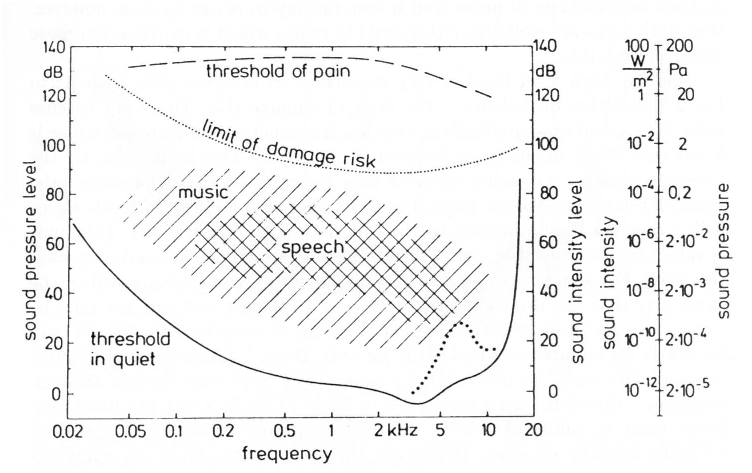
\includegraphics{Graph/hoerfl}
\caption[Darstellung der H�rfl�che]{H�rfl�che, d.h. Fl�che zwischen Ruheh�rschwelle und Schmerzgrenze. Zus�tzlich ist
zur Orientierung die typische Fl�che f�r Sprache und Musik skizziert (aus \cite{zwicker})}
\label{fig:hoerflaeche}
\end{center}
\end{figure}
\bem{Neben den oben genannten Gr��en ist in Abb. \ref{fig:hoerflaeche} auch die Risikogrenze f�r
Geh�rsch�den angegeben. Diese Gr��e geht allerdings von einer dauerhaften Belastung ($8$
Stunden am Tag, $5$ Tage die Woche) aus; der Schalldruckpegel kann etwas erh�ht werden,
wenn die Dauer der Belastung verk�rzt wird. Wird das Ohr hohen Belastungen ausgesetzt, so
kommt es zu einer vor�bergehenden Verschiebung der Grenzen der H�rfl�che zu h�heren Pegeln.
Geschieht dies aber �fters, so wird die tempor�re Verschiebung zu einer permanenten, also
einem Geh�rschaden.}\end{quote}

\chaplink
\begin{itemize}
	\item Abschnitt \ref{chap:amplitude}
	\item Abschnitt \ref{chap:lautstaerke}
\end{itemize}
\end{quote}

\section{Pegel bei der Addition von Signalen}\label{chap:leveladd}\begin{sloppypar}
Bis jetzt wurde noch nicht be\-handelt, wie hoch der Pe\-gel ei\-nes Si\-gnals
$u(t)=x(t)+y(t)$ ist, das die Summe zweier Signale darstellt. Wie in Abschnitt
\ref{chap:ss-pegel} ausgef�hrt, steht im Argument des Logarithmus ein Effektivwert. Leider
lassen sich Effektivwerte resp. Leistungen nicht so einfach addieren, wie man das
vielleicht erwarten k�nnte. Es zeigt sich n�mlich, da� es bei der Addition eine Rolle
spielt, ob sich die Signale, welche addiert werden, \textit{�hnlich} sind oder nicht. \\
\end{sloppypar}
Zur Erl�uterung m�ssen erst einige Begriffe eingef�hrt werden, die leider anschaulich
schwer zu fassen sind.\footnote{Es kann sein, da� diese Begriffe an anderer Stelle anders
eingef�hrt werden. Es wurde versucht, die Definition der beiden Begriffe Inkoh�renz und
Korrelation m�glichst aus dem g�ngigen Gebrauch in der Aufnahmepraxis herzuleiten. Aus
diesem Grund mu� man sich bei der Lekt�re verschiedener Literatur immer vergewissern, in
welchem Sinn die Begriffe Koh�renz\index{Koh�renz} und Korrelation\index{Korrelation}
benutzt werden.} Zwei Signale hei�en koh�rent\index{Koh�renz}, wenn ein Signal nur gegen
sich selber verschoben und skaliert wurde, beispielsweise wenn sie von der gleichen Quelle
kommen. Laufzeit- bzw. Pegelunterschiede spielen also keine Rolle.\\ Zwei Signale hei�en
hingegen inkoh�rent\index{Inkoh�renz}, wenn sie einander zu keinem Zeitpunkt in irgendeiner
Weise �hnlich sind.\\ Die Korrelation\index{Korrelation} gibt die Verwandtschaft zweier
Signale zu einem bestimmten Zeitpunkt pegelunabh�ngig an. Signale sind also korreliert,
wenn sie bis auf einen Skalierungsfaktor �bereinstimmen. Der sogenannte
Korrelationsgrad\index{Korrelationsgrad} zeigt die �hnlichkeit auf einer Skala zwischen
$[-1;1]$ an; dabei steht \glqq$1$\grqq$\:$  f�r Gleichheit,
\glqq$-1$\grqq$\:$  f�r Gegenphasigkeit und \glqq$0$\grqq$\:$  f�r Unkorreliertheit.\\ Dies bedeutet
einerseits, da� inkoh�rente Signale immer unkorreliert sind, andererseits korrelierte
Signale immer koh�rent sind. Umgekehrt trifft dies nicht allgemein zu.

\bsp{Rauschen ist zu allen Signalen (au�er zu sich selbst) inkoh�rent und damit auch
unkorreliert.\\ Eine Sinus- und eine Cosinusschwingung sind zwar unkorreliert zueinander,
aber koh�rent.\\ Die Ausgangssignale zweier Mikrophone sind (wenn die Mikrophone nicht zu
nah beieinander stehen) n�herungsweise unkorreliert.}\end{quote}
\bem{In der Technik und Mathematik wird oft der Begriff \textit{orthogonal} statt
\textit{nicht korreliert} verwendet. Die Bedingung f�r Unkorreliertheit bzw. Orthogonalit�t zweier
Signale $x(t),y(t)$ ist $\int x(t)\cdot y(t)\,dt=0$}\end{quote}

Man stelle sich nun die zu addierenden Signale als Vektoren vor (s. Abb. \ref{fig:effadd}),
deren Betrag ihr Effektivwert ist. Sind zwei Signale identisch, so haben die zugeh�rigen
Vektoren den gleichen Betrag und die gleiche Orientierung. Sind sie hingegen unkorreliert,
so stehen die Vektoren senkrecht aufeinander (90� Phasenverschiebung!). Das gew�nschte
Ergebnis, n�mlich der Effektivwert des resultierenden Signals, ist der Betrag des aus der
Addition resultierenden Vektors.

\begin{figure}[!hbt]
\begin{picture}(50,40)
\put(15,30){$Addition\: gleicher\: Signale$} \multiput(35,3)(0,10){2}{\vector(0,1){10}}
\put(36,3){\vector(0,1){20}} \put(25,8){$x_{eff,1}$} \put(25,18){$x_{eff,2}$}
\put(38,11){$x_{eff,Ges}$}

\put(70,30){$Addition\: unkorrelierter\: Signale$} \put(90,10){\vector(1,0){5}}
\put(90,10){\vector(0,1){10}} \put(90,10){\vector(1,2){5}} \put(80,15){$x_{eff,2}$}
\put(90,6){$x_{eff,1}$} \put(96,20){$x_{eff,Ges}$}

\end{picture}
\caption{Veranschaulichung der Addition von Effektivwerten}\label{fig:effadd}
\end{figure}

F�r die Addition zweier gleicher Signale $x$ erh�lt man also
\begin{equation}\label{vektoradd1}
  u_{Ges,eff}=2\cdot x_{eff}
\end{equation}
Der Pegel des resultierenden Signals nimmt also um $\mathbf{20\log{2}=6\; [dB]}$ zu.\\ Bei
der Addition zweier nicht korrelierter Signale $x$ und $y$ erhalten wir
\begin{equation}\label{vektoradd2}
  u_{Ges,eff}=\sqrt{x_{eff}^2+y_{eff}^2}
\end{equation}
F�r $x_{eff}=y_{eff}$ erh�lt man hier eine Zunahme um $\mathbf{20\log{\sqrt{2}}=3\; [dB]}$!
Bei der Addition von unkorrelierten Signalen \textit{gleichen} Pegels nimmt der Pegel also
um $3 dB$ zu.
\bsp{Das Rauschen
zweier Tonbandspuren, die mit gleichem Pegel gemischt werden, ist um $3dB$ lauter als das
einer Spur.}
\end{quote}


Werden nun mehrere nicht korrelierte Quellen \textit{gleichen} Pegels addiert, so erh�lt
man analog dazu:
\begin{equation}\label{eq:vektoradd3}
  u_{Ges,eff}=\sqrt{u_{1,eff}^2+u_{2,eff}^2+\ldots+u_{n,eff}^2}
\end{equation}
und der Gesamtpegel nimmt dementsprechend um $20\log{\sqrt{n}}=10\log{n}\; [dB]$ zu.\\ Haben
die Quellen nicht denselben Pegel, so mu� man in die obigen Gleichungen die entsprechenden
Effektivwerte einsetzen und hat etwas mehr Arbeit. Die Rechnung ist aber im Prinzip
identisch.

\bem{Es gibt nat�rlich beliebige Zwischenstufen zwischen \glqq unkorreliert\grqq$\;$ und \glqq identisch\grqq$\;$ (s. Abb\ref{fig:pegeladd}). In einem
solchen Fall stehen die Vektoren dann nicht mehr senkrecht aufeinander und der
resultierende Pegel wird bei der Addition von zwei Signalen zwischen $3$ und $6dB$ liegen.}
\end{quote}
\begin{figure}[!hbt]
\begin{center}
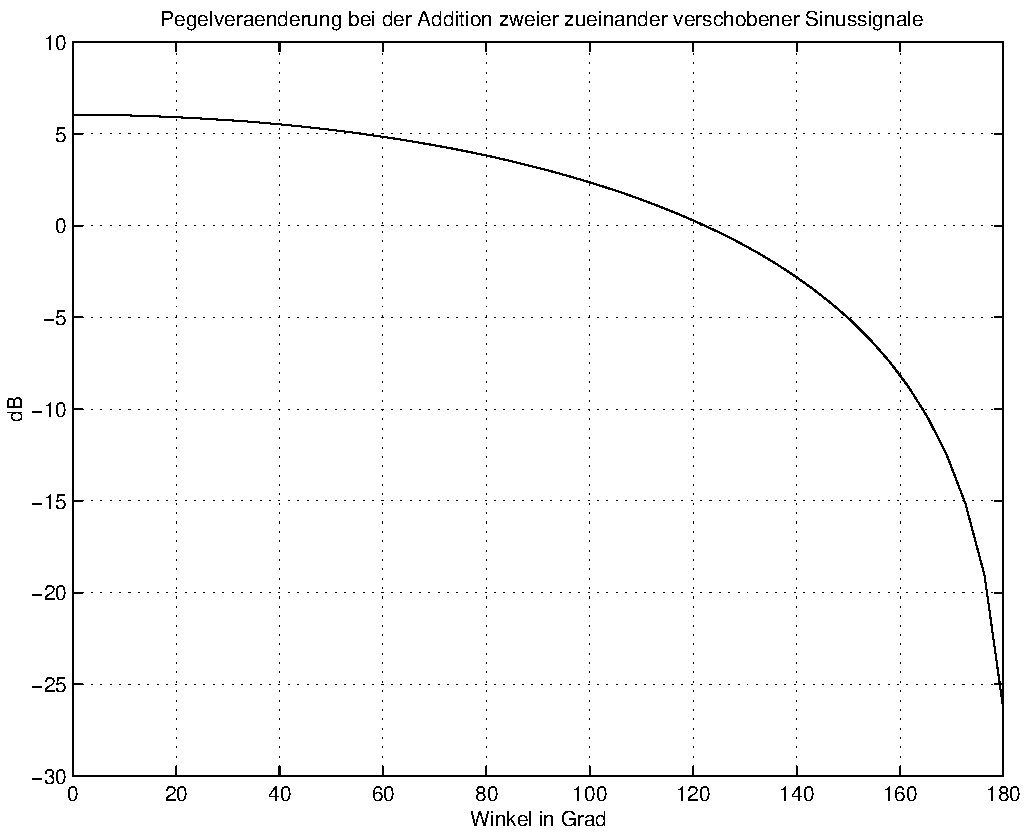
\includegraphics[scale=.5]{Graph/pegeldif}
\caption[Addition zueinander verschobener Sinusignale]{Pegel�nderung bei der Addition zweier zueinander verschobener Sinussignale. F�r
einen Phasenwinkel von 0� ergeben sich 6dB Pegelzunahme, w�hrend der Pegel des
resultierenden Signals f�r einen Winkel von $180$� gegen $-\infty$ geht}
\label{fig:pegeladd}
\end{center}
\end{figure}

F�r die Leser, die es etwas genauer wissen wollen, folgt eine etwas detailliertere
Herleitung.
\herl{Um die erhaltenen Resultate zu �berpr�fen, mu� die Definition
des Effektivwertes betrachtet werden, die ja lautete
\begin{equation}\label{effektiv}
  u_{eff}=\sqrt{\lim_{T \rightarrow \infty} \frac{1}{T}\int_{T} \left[u(t)\right]^2\,dt}.
\end{equation}
Dementsprechend gilt also f�r den Effektivwert, wenn $u(t)$ die Summe zweier Signale $x(t)
$ und $ y(t)$ ist
\begin{eqnarray}\label{effektiv2}
  u_{eff} &=&\sqrt{ \lim_{T \rightarrow \infty} \frac{1}{T}\int_{T} \left[x(t)+ y(t)\right]^2\,dt}\nonumber\\
  &=&\sqrt{ \lim_{T \rightarrow \infty} \frac{1}{T}\int_{T} \left[x(t)^2+y(t)^2+2x(t)y(t)\right]\,dt}.
\end{eqnarray}
F�r den Fall, da� $x(t)=y(t)$ ist, erh�lt man
\begin{eqnarray}\label{effektiv3}
  u_{eff}&=&\sqrt{ \lim_{T \rightarrow \infty} \frac{1}{T}\int_{T} \left[2\cdot x(t)\right]^2\,dt}\nonumber\\
   &=&2\cdot x_{eff},
\end{eqnarray}
also das Ergebnis, das nach Gleichung \ref{vektoradd1} schon erwartet werden konnte.\\

Sind $x$ und $y$ nicht korreliert, so gilt f�r die Gleichung \ref{effektiv2}, da� das
Integral �ber den gemischten Term gleich $0$ ist (dies gilt aufgrund der
Ortho\-gonali\-t�ts\-eigen\-schaft, die als mathematische Definition der Unkorreliertheit gegeben
wurde). Mit Hilfe der Orthogonalit�tseigenschaft unkorrelierter Signale folgt also
\begin{equation}
  u_{eff} = \sqrt{x_{eff}^2+y_{eff}^2}
 \end{equation}
und damit Gleichung \ref{vektoradd2}.}
\end{quote}

Bisher ging es um die \textit{elektrische} Addition von Signalen. Sollen diese
\textit{akustisch} addiert werden, so ergeben sich andere Pegelunterschiede. Im allgemeinen sind Schallwellen im Raum bei zwei Sendern nicht mehr korreliert, auch wenn die Sender selbst das gleiche Signal abstrahlen.
Dementsprechend erh�ht sich der Schalldruckpegel bei zwei Lautsprechern, welche das gleiche
Signal abstrahlen, um $3dB$.
\bsp{Zwei Lautsprecher, die mit dem gleichen Signal gespeist werden, erzeugen einen
Schalldruckpegel, der um $3dB$ h�her ist als der von einem einzigen Lautsprecher erzeugte
Pegel.\\ Zwei gleiche und gleichlaute Musikinstrumente spielen unisono $3dB$ lauter als ein
einzelnes.}\end{quote}

\section{Zusammenfassung}
Es wurde eine (Pseudo-)Einheit \textbf{Dezibel} eingef�hrt. Mit dieser Einheit lassen sich
viele Gr��en dem menschlichen Empfindungsverm�gen aufgrund des Weber-Fechnersche Gesetzes
anpassen. \textit{Dezibel} ist keine richtige Einheit, sondern kann sowohl f�r
Pegeldifferenzen (relative Pegel) als auch f�r absolute Gr��en (bezogen auf einen
Bezugswert) stehen. Eine besonders wichtige Gr��e f�r Tonmeister ist der
\textbf{Schalldruckpegel}. Dessen Bezugsgr��e ist $2\cdot 10^{-5}Pa$.
\\ Jeder absolute Pegel ist auf eine bestimmte Bezugsgr��e normiert. Nur bei Kenntnis
dieser Bezugsgr��e ist eine Angabe eines beliebigen Wertes in $dB$ sinnvoll.
\\ Der resultierende Pegel bei der Addition von Signalen ist \textit{nicht} die Summe der
Einzelpegel. Um den resultierenden Pegel berechnen zu k�nnen, mu� zuerst der resultierende
Effektivwert errechnet werden, daraufhin kann auch der Pegel bestimmt werden. Bei der
elektrischen Addition zweier Signale gleichen Pegels ergibt sich $6dB$, falls die Signale
korreliert sind, und $3dB$ im unkorrelierten Fall. Bei der akustischen Addition zweier
Signale ergibt sich hingegen i.a. eine Pegelerh�hung von $3dB$.

\section{Aufgaben}
Vor den Aufgaben eine kurze Wiederholung der wichtigsten Eigenschaften der
Logarithmusrechnung:
\begin{quote}\footnotesize
\begin{itemize}
         \item $\log{(a\cdot x)}=\log{a}+\log{x}$
         \item $\log{x^{a}}=a\cdot \log{x}$
         \item $x=10^{\log{x}}$
         \item $\log{x}=\frac{\ln{x}}{\ln{10}}$
         \item $\log\frac{1}{x}=-\log{x}$
         \item Ableitung $\partial\frac{\log{x}}{\partial x}	= \frac{1}{x}$
\end{itemize}
\end{quote}

\begin{enumerate}

\item  Leite aus Gleichung \ref{eq:weber} das Weber-Fechner-Gesetz $W=const.\cdot ln(R)+C$ her.

\item  Wie gro� ist die Abnahme des Schalldrucks und des Schalldruckpegels bei
einer Verdoppelung der Entfernung, wenn der Schalldruck proportional $1/r$ abnimmt?

\item  Berechne f�r folgende Spannungsverh�ltnisse  die Pegeldifferenz in $dB$:
\begin{itemize}
	\item $1:1$
	\item $1:\sqrt{2}$
	\item $1:2$
	\item $1:10$
\end{itemize}

\item  Berechne f�r folgende Pegeldifferenzen die Spannungsverh�ltnisse:
\begin{itemize}
	\item $3dB$
	\item $6dB$
	\item $10dB$
	\item $20dB$
	\item $100dB$
\end{itemize}

\item  Berechne die Pegelzunahme bei der Addition von $4$ bzw. $8$ unkorrelierten Quellen
gleichen Pegels.

\item  Welcher Pegelunterschied ergibt sich zwischen den Ausgangsspannungen zweier Mikrophone (Schalldruckempf�ngern), die 60cm und 180cm von der Schallquelle entfernt sind?

\item  Um wieviel Dezibel nimmt der Pegel zu, wenn statt $2$ Lautsprechern $4$ von dem gleichen Signal angesteuert werden?

\item  Um wieviel Dezibel nimmt der Pegel zu, wenn statt $5$ Geigen $10$ spielen?

\item  Berechne sowohl f�r den korrelierten (\glqq gleichen\grqq) als auch f�r den unkorrelierten Fall die Pegelzunahme bei der Addition zweier Signale, deren Pegelunterschied
\begin{itemize}
	\item $6dB$
	\item $10dB$ betr�gt.
\end{itemize}
\end{enumerate}

% m�gliche Ger�te: Korr-messer, Goniometer, RTW, VU-meter
	\chapter{Raumakustik}\label{chap:raumak}
\thispagestyle{empty}

Die Akustik eines Aufnahmeraums kann f�r die Klangqualit�t einer Aufnahme von entscheidender Bedeutung sein. Das folgende Kapitel gibt eine �bersicht �ber die wichtigsten Gr��en der Raumakustik und akustische Besonderheiten bestimmter R�ume.

In einem Raum erreicht nicht nur der Schall das Ohr des H�rers, der von der Schallquelle
den direkten Weg nimmt , sondern auch vielf�ltige Reflexionen von W�nden, Decke, Boden,
etc. Diese Reflexionen erzeugen einen Raumeindruck, der sich von Raum zu Raum stark
unterscheidet. Dieser Raumeindruck, also die \textit{Akustik} des Raumes, wird dadurch
festgelegt, wann, wie stark und wie h�ufig Reflexionen im Vergleich zum Direktschall beim
H�rer eintreffen (s. Abb. \ref{fig:raumIR}). 

\begin{figure}[!hbt]
\begin{center}
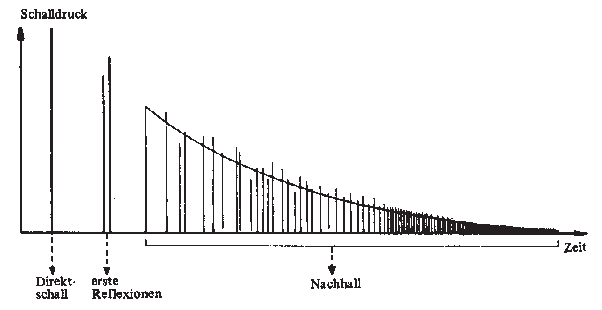
\includegraphics[scale=.9]{Graph/impuls}
\caption[Reflexionsverhalten eines Raumes]{Zeitliche Folge der Reflexionen in einem Raum bei Impulsschall (aus \cite{dickr})}
\label{fig:raumIR}
\end{center}
\end{figure}
Im allgemeinen treffen die ersten Reflexionen nach dem Direktschall relativ vereinzelt ein
und bestimmen durch ihre Verz�gerung zum Direktschall und ihren Pegel stark den
Klangeindruck des Raumes. Mit zunehmender Zeit liegen die einzelnen Reflexionen immer
dichter beieinander und \glqq verschwimmen\grqq$\:$  zu einem abklingenden Nachhall.

\bem{Tats�chlich ist die Verz�gerung und St�rke der eintreffenden Reflexionen sowohl vom
Standort des H�rers als auch von dem der Schallquelle abh�ngig. Das bedeutet nichts
anderes, als da� verschiedene Punkte in einem Saal unterschiedliche H�reindr�cke
hervorrufen k�nnen. Es gibt aber doch einen mittleren Gesamteindruck des Raumes, den man
meint, wenn man allgemein von der Akustik eines Raumes spricht.}\end{quote}
	\ifthenelse{\equal{\value{allchaps}}{1}}
{
\chaplink
\begin{itemize}
	\item Abschnitt \ref{chap:reverb}
\end{itemize}
\end{quote}
}{}

\section{Nachhallzeit}\label{chap:nachhallzeit}
Die \textbf{Nachhallzeit}\index{Nachhallzeit} $T$ ist eines der wichtigsten und
bekanntesten Kriterien zur Beurteilung der Akustik eines Raumes. Sie als die Zeit
definiert, in der die Schallenergie eines (eingeschwungenen) Raumes nach \glqq
Abschalten\grqq$\:$  der Schallquelle auf den millionensten Teil, d.h. um $60dB$ abnimmt. Diese
Zeit entspricht nicht unbedingt der vom Zuh�rer tats�chlich geh�rten Zeit des Ausklangs,
der \textbf{Nachhalldauer}\index{Nachhalldauer}, da diese abh�ngig von der Lautst�rke der
Schallquelle ist\footnote{So ist die
\textit{Nachhalldauer} beispielsweise f�r ein Fingerschnippen sicherlich geringer als f�r
ein Klatschen, die
\textit{Nachhallzeit} des Raumes bleibt aber dennoch immer die gleiche}. Abh�ngig vom Volumen eines Raumes
und den Absorptionseigenschaften des Wandmaterials ergeben sich f�r verschiedene R�ume
stark unterschiedliche Nachhallzeiten. Der Akustiker \textit{Sabine} fand empirisch die
\textit{Sabinesche Nachhallformel} zur n�herungsweisen rechnerischen Ermittlung der
Nachhallzeit:
\begin{equation}\label{eq:nachhall}
  T\simeq 0.163sm^{-1}\frac{V}{A}
\end{equation}

\begin{quote}\begin{footnotesize}
$V$ ist das Volumen des Raumes\\ $A$ ist die sogenannte �quivalente Absorptionsfl�che, d.h.
die Summe aller Einzelfl�chen multipliziert mit ihrem jeweiligen Absorptionsgrad. Die Gr��e
der Fl�che $A$ entspricht also der Gr��e einer theoretischen Fl�che, welche keinen Schall
reflektiert.
\end{footnotesize}\end{quote}

\begin{sloppypar}
R�ume f�r unterschiedliche Anwendungen sollten auch unterschiedliche Nachhallzeiten haben.
So mu� beispielsweise ein Theater wesentlich \glqq trockener\grqq$\:$  sein als ein
Konzertsaal, um die Sprachverst�ndlichkeit zu erh�hen. Typische Nachhallzeiten liegen in
Konzerts�len oft um die $2s$, in Theatern um $1.2s$ und in Kirchen sehr variabel von ca.
$3s$ bis zu $7s$.\\
\end{sloppypar}

Der Nachhall klingt n�herungsweise exponentiell ab; wenn man also den Schall\-druckpegel �ber
der Zeit auftr�gt, so erkennt man eine abfallende Gerade, die \textit{Nachhallgerade} (s.
Abb. \ref{fig:rt-gerade}).

\begin{figure}[!hbt]
\begin{center}
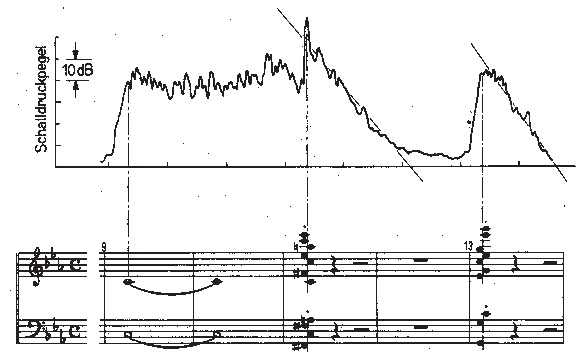
\includegraphics{Graph/rt-gerad}
\caption[Nachhall w�hrend eines Konzerts]{Nachhallaufzeichnung mit Pegelschreiber w�hrend eines Konzerts (Beethoven Op.62,
Coriolan-Ouvert�re, Takt 9 ff) (aus \cite{raumakustik})} \label{fig:rt-gerade}
\end{center}
\end{figure}

\section{Absorption}\index{Absorption}\label{chap:absorption}

\section{Direktschallfeld und Diffusschallfeld}\label{chap:freifeld}\begin{sloppypar}
Der \textbf{Direktschall}\index{Direktschall} ist derjenige Schall, der den direkten Weg
vom Sender zum H�rer nimmt, also als erste Wellenfront vom Sender eintrifft. Der
\textbf{Diffusschall}\index{Diffusschall} oder Raumschall ist der Schall, der bei seinem Eintreffen beim H�rer
bereits eine oder mehrere Reflexionen erfahren hat. Der Direktschall nimmt nach Gleichung
(\ref{eq:r-gesetz}) mit zunehmender Entfernung von der Schallquelle ab und bildet das sogenannte
\textbf{Direktschallfeld}\index{Direktschallfeld} oder
\textbf{Freifeld}\index{Freifeld}. Hingegen spricht man von \textbf{diffusem Schallfeld}\index{Diffusschallfeld} oder statistischem
Schallfeld, wenn der Schalleinfall am Me�ort aus allen Raumrichtungen gleich wahrscheinlich
und gleich stark ist. Das bedeutet, da� im rein diffusen Schallfeld keine Lokalisation der
Schallquelle mehr m�glich ist. Der Pegel des Diffusschallfeldes ist bei l�ngeren
Nachhallzeiten im gesamten Raum gleich, h�ngt also nicht von der Entfernung zur
Schallquelle ab (s. Abb. \ref{fig:direktdiffus}).\\
\end{sloppypar}
\bem{Die Begriffe Direktschallfeld und Diffusschallfeld sind nicht zu verwechseln mit
Nahfeld und Fernfeld, sondern stehen f�r etwas vollkommen anderes!}
\end{quote}

\begin{figure}[!hbt]
\begin{center}
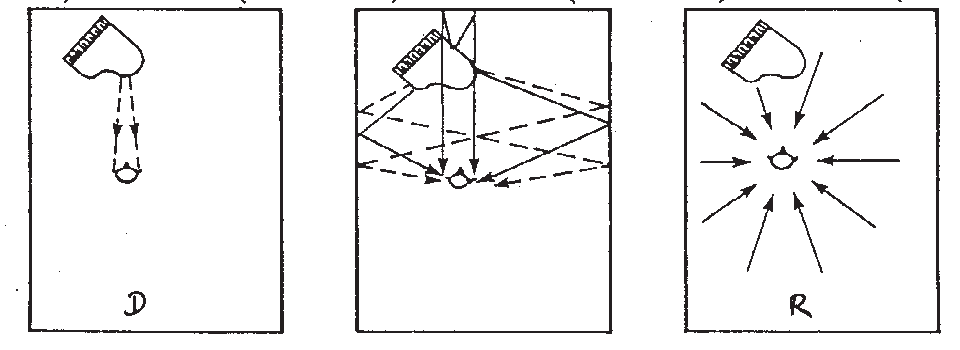
\includegraphics[scale=.9]{Graph/dirdiff}
\caption[Direktschall, erste Reflexionen und Diffusschall am Ort des H�rers]{Direktschall, erste Reflexionen und Diffusschall am Ort des H�rers (aus
\cite{sengpiel})} \label{fig:direktdiffus}
\end{center}
\end{figure}

\section{Hallradius}\label{chap:hallradius}
In einem Raum �berlagern sich Direktschallfeld und Diffusschallfeld. Nahe an der
Schallquelle ist das Direktschallfeld stark im Vergleich zum Diffusschallfeld. Je weiter
man sich allerdings von der Quelle entfernt, desto schw�cher wird der Pegel des
Direktschalls und \glqq verschwindet\grqq$\:$  irgendwann im Diffusschall, der ja im gesamten
Raum den gleichen Pegel hat (s. Abb. \ref{fig:hallrad}). Die Entfernung von der
Schallquelle, bei welcher der Schallpegel des Direktschalles gleich dem des Raumschalles
ist, wird \textbf{Hallradius}\index{Hallradius} genannt:
\begin{equation}\label{eq:hallrad}
  r_{H}=0.057s^{1/2}m^{-1/2}\sqrt{\frac{V}{T}}
\end{equation}
\begin{quote}
\footnotesize{
$r_{H}$ ist der Hallradius\\ $V$ ist das Volumen des Raumes\\ $T$ ist die Nachhallzeit des
Raumes}
\end{quote}

%Vielleicht ist Dickreiter, p.37 geeigneter??

\begin{figure}[!hbt]
\begin{center}
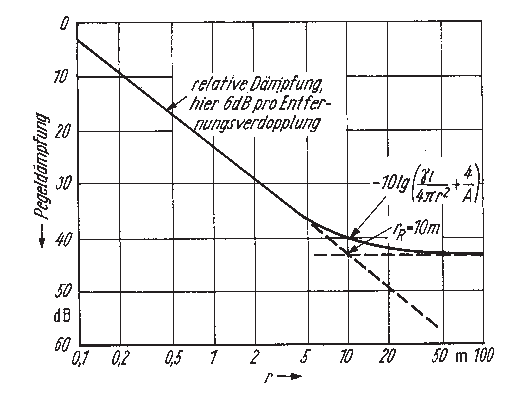
\includegraphics{Graph/hallrad}
\caption[Pegeld�mpfung �ber der Entfernung von der Schallquelle]{Pegeld�mpfung in einem trockenen Raum �ber der Entfernung von der Schallquelle. Der Schallpegel verh�lt sich f�r kleine Abst�nde nach dem 1/r-Gesetz, f�r gro�e
Abst�nde ist er gleich dem Diffusschallpegel (aus \cite{ahnert})} \label{fig:hallrad}
\end{center}
\end{figure}

\begin{sloppypar}
Bei einer Vergr��erung des Raumvolumens steigt der Hallradius also an, bei einer
Verl�ngerung der Nachhallzeit verringert er sich (s. Abb. \ref{fig:hallrad2}). Die sich aus
dieser Gleichung ergebenden Hallradien sind erstaunlich gering; so betr�gt er in einem
$100m^3$ gro�en Zimmer mit der Nachhallzeit $0.5s$ lediglich $81cm$.\\
\end{sloppypar}

\begin{figure}[!hbt]
\begin{center}
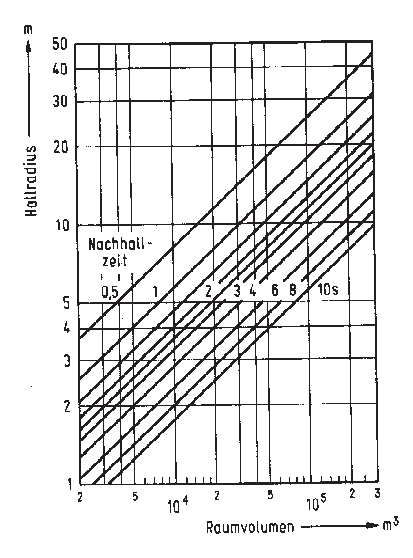
\includegraphics{Graph/hallrad2}
\caption[Hallradien in Abh�ngigkeit von Raumvolumen und Nachhallzeit]{Hallradien in Abh�ngigkeit von Raumvolumen und Nachhallzeit (aus \cite{webers})}
\label{fig:hallrad2}
\end{center}
\end{figure}

Wie schon der Name Hall\textit{radius} impliziert, gilt diese Definition nur f�r eine
vollkommen ungerichtete Schallabstrahlung (Kugelschallquelle). Da die meisten Schallquellen
in der Regel aber nicht kugelf�rmig abstrahlen, erweitert man Gleichung (\ref{eq:hallrad}) um
den sogenannten \textit{B�ndelungsgrad}\index{B�ndelungsgrad} \footnote{Der
B�ndelungsgrad ist f�r eine Kugelschallquelle $1$ und wird gr��er, je st�rker eine Quelle
gerichtet abstrahlt.} $\gamma$ und erh�lt in Hauptabstrahlrichtung der Schallquelle
\begin{equation}\label{eq:hallrad2}
  r_{H,eff}=0.057s^{1/2}m^{-1/2}\sqrt{\gamma}\sqrt{\frac{V}{T}}.
\end{equation}
\begin{sloppypar}
Dieser Wert wird als \textit{effektiver Hallradius}\index{Hallradius!effektiver},
\textit{Hallabstand}\index{Hallabstand} oder seltener als
\textit{Richtentfernung}\index{Richtentfernung} bezeichnet.
\bem{F�r Aufnahmen ist die Kenntnis des Hallradius eines Raumes insofern wichtig, als man schon beim Aufstellen der Mikrophone
ansatzweise einsch�tzen kann, ab welcher Entfernung von der Schallquelle der Direktschall
leiser als der Diffusschall sein wird. Mit diesem Wissen lassen sich die Mikrophone schon
vor dem ersten Testh�ren an einem Ort aufstellen, der der angestrebten Aufnahme�sthetik
bez�glich des Verh�ltnisses von Direktschall und Raumanteil in etwa entsprechen k�nnte.
Eine solche �berlegung kann aber nur erste Anhaltspunkte f�r den Mikrophonstandort
liefern.}\end{quote}
\end{sloppypar}


\section{Frequenzabh�ngigkeit des Nachhalls}
Die Nachhallzeit\index{Nachhallzeit} wurde oben als die Zeit definiert, in der die Energie eines eingeschwungenen Raumes um $60dB$ abnimmt (s. Abschnitt \ref{chap:nachhallzeit}). Nun klingen allerdings auch R�ume mit identischer Nachhallzeit oftmals sehr unterschiedlich. Die Nachhallzeit ist n�mlich nicht f�r alle Frequenzen konstant, sondern unterscheidet sich zum Teil stark f�r verschiedene Frequenzen. In den meisten R�umen ist die Nachhallzeit bei tiefen Frequenzen l�nger als bei h�heren Frequenzen. Eine Messung der frequenzabh�ngigen Nachhallzeit ist pr�ziser und aussagekr�ftiger als die Messung der frequenzunabh�ngigen Nachhallzeit.


\section{Flatterecho}
Breitet ein Schallsignal sich derart aus, da� es �ber zwei (oder mehrere) Fl�chen wieder an
den Ausgangspunkt zur�ckkehrt, so kann ein \textbf{Flatterecho}\index{Flatterecho}
entstehen. Das bedeutet, da� der Schall immer wieder hin- und hergeworfen wird und somit -
bei einem impulsartigem Schallereignis (Klatschen, etc.) - eine schnelle Abfolge leiser
werdender Echos wahrzunehmen ist. Diese Echos werden i.a. als st�rend empfunden. Ein
Flatterecho kann insbesondere dann entstehen, wenn zwei reflektierende W�nde parallel
zueinander stehen und die anderen Raumrichtungen st�rker ged�mpft sind. \\ Um ein
Flatterecho zu beseitigen, sollte man entweder versuchen, eine der beiden
gegen�berstehenden W�nde z.B. durch einen Vorhang absorbierend zu machen, oder mit Hilfe
von Diffusoren, gro�en Stellw�nden etc. die Reflexionen in andere Richtungen abzulenken.
Oft hilft auch einfach nur eine andere Plazierung der Musiker bzw. der Mikrophone.

\section{Stehende Wellen}
Trifft eine Schallwelle senkrecht auf eine Wand (Einfallsrichtung 0�), so �berlagern sich
die einfallende und die reflektierte Welle. \\ Man stelle sich nun zwei parallel stehende
reflektierende W�nde vor; entspricht eine halbe Wellenl�nge oder ein Vielfaches davon genau
dem Abstand der beiden W�nde, so werden sich Direktschall und ein- bzw. mehrfach
reflektierter Schall immer phasengleich �berlagern. Lediglich die Ausbreitungsrichtung kann
unterschiedlich sein. Es entsteht ein station�res Schallfeld zwischen den beiden W�nden mit
Schwingungsknoten, in denen der Schalldruck fast $0$ ist und Schwingungsb�uchen, in denen
er maximal ist; diese sind ortsfest und ver�ndern sich nicht �ber der Zeit. Dies sind
sogenannte \textbf{stehende Wellen}\index{Welle!stehende} (s. Abb. \ref{fig:stehwelle1}); sie werden teilweise auch als \textit{Raumresonanzen} oder
\textit{Raummoden}\index{Raummode} bezeichnet.
\begin{figure}[!hbt]
\begin{center}
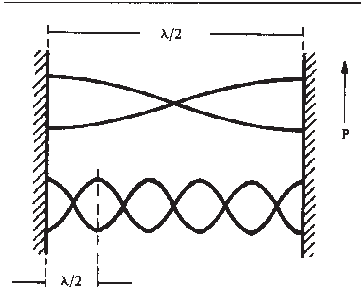
\includegraphics{Graph/stwelle1}
\caption[Druckverteilung in stehenden Wellen zwischen zwei W�nden]{Druckverteilung in stehenden Wellen zwischen zwei parallelen W�nden f�r zwei verschiedene Frequenzen (aus
\cite{dickr})} \label{fig:stehwelle1}
\end{center}
\end{figure}

\bem{Stehende Wellen k�nnen nicht nur zwischen zwei parallel stehenden W�nden auftreten,
sondern auch durch mehrfache Reflexionen an verschiedenen W�nden, wenn die Bedingung
erf�llt ist, da� der zur�ckgelegte Weg ein Vielfaches der halben Wellenl�nge ist. Solche
stehenden Wellen werden dann Raummoden h�herer Ordnung genannt.}\end{quote}

Abbildung \ref{fig:stehwelle2} zeigt den Zusammenhang zwischen Druck und Schnelle bei einer
stehenden Welle.
\begin{figure}[!hbt]
\begin{center}
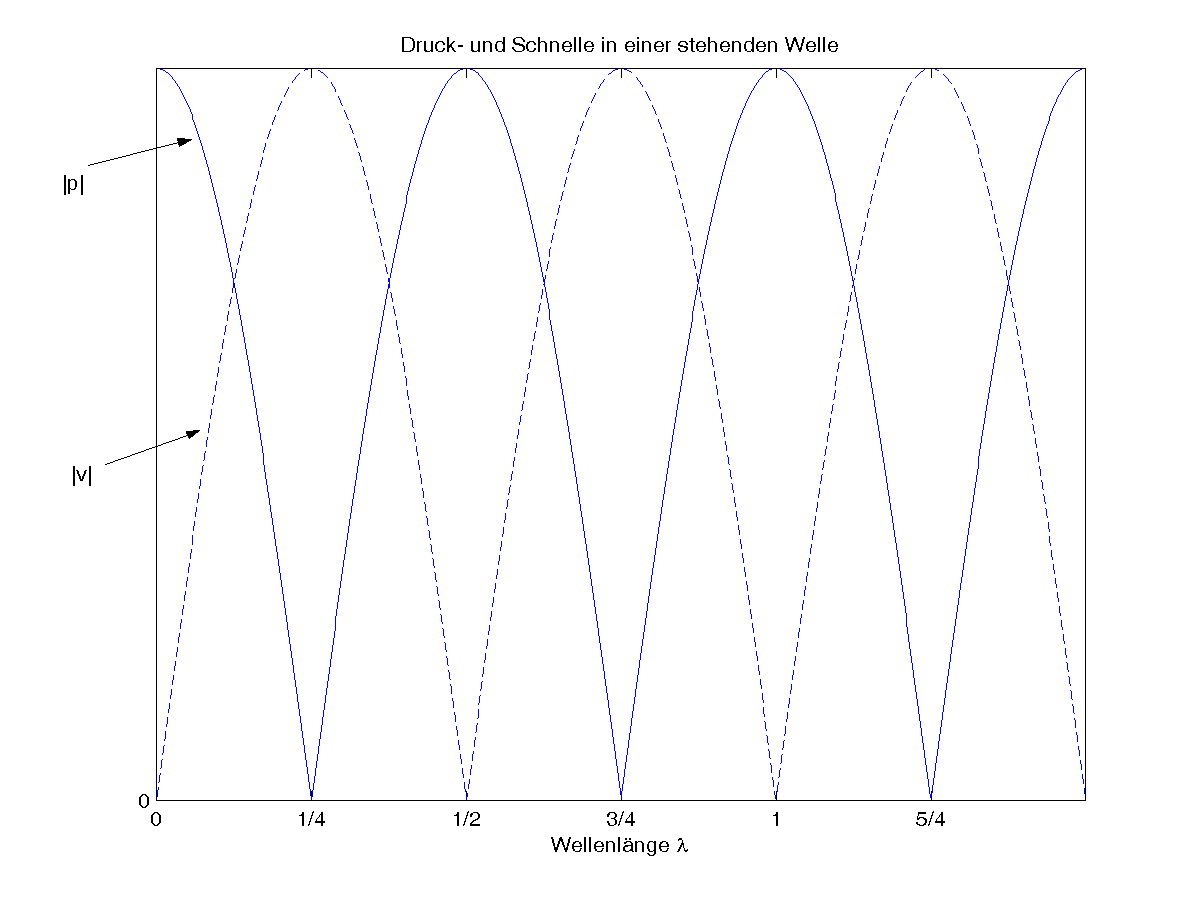
\includegraphics[scale=.5]{Graph/mstwelle2}
\caption{Druck- und Schnelleverlauf in einer stehenden Welle} \label{fig:stehwelle2}
\end{center}
\end{figure}


Stehende Wellen fallen vor allem in kleineren R�umen bei tiefen Frequenzen auf. Bei hohen
Frequenzen liegen die Schwingungsknoten und -b�uche so dicht nebeneinander, da� man sie
nicht mehr wahrnehmen kann. Je kleiner ein Raum ist, desto weiter liegen die Frequenzen
auseinander, bei denen sich stehende Wellen ausbilden k�nnen. Deshalb kann man stehende
Wellen in kleinen R�umen deutlicher wahrnehmen, da sie sich nur bei sehr wenigen Frequenzen
ausbilden, die sich vom H�rer deutlich unterscheiden lassen. Aus diesem Grund wird bei der
akustischen Konzeption eines Raumes darauf geachtet, da� die sogenannte
\textit{Eigenfrequenzdichte} m�glichst hoch ist, d.h. da� die Frequenzen der einzelnen
Moden m�glichst so dicht nebeneinander liegen, da� die Wahrnehmung einer einzelnen Mode
nicht mehr wahrnehmbar ist.

\begin{sloppypar}
\bem{Theoretisch tritt das Problem von stehenden Wellen erst auf, wenn der Raum mit einem
reinen Sinuston dauerhaft angeregt wird, und nicht bei zeitlich ver�nderlichen
(Musik-)Signalen. Tats�chlich kann es bei einer Aufnahme jedoch passieren, da� eine gewisse
Ba�lastigkeit oder Ba�armut auftritt, die dann durch leichtes Verr�cken der Mikrophone
verschwinden kann.}\end{quote}
\end{sloppypar}

\section{Zusammenfassung}
Die sogenannte Akustik eines Raumes wird gekennzeichnet durch den Pegel, die Zeit und die
Anzahl, mit der Reflexionen im Vergleich zum Direktschall beim Zuh�rer eintreffen. Ein sehr
wichtiges Kriterium f�r den Gr��eneindruck des Raumes ist die \textbf{Nachhallzeit} $T$.
Sie ist abh�ngig von dem Raumvolumen und der Menge und Art von absorbierendem Material im
Raum und entspricht im allgemeinen nicht der tats�chlich geh�rten \textbf{Nachhalldauer}. Die Nachhallzeit ist \textbf{frequenzabh�ngig}, d.h. verschiedene Frequenzen klingen unterschiedlich schnell nach. Im allgemeinen ist die Nachhallzeit bei tiefen Frequenzen l�nger als bei hohen.\\
Durch die vielf�ltigen Reflexionen an den Begrenzungsfl�chen entsteht zus�tzlich zu dem von
der Schallquelle ausgesendeten \textbf{Direktschallfeld} ein n�herungsweise
\textbf{diffuses Schallfeld}. Hier trifft der Schall von allen Seiten gleich stark und mit
gleicher Wahrscheinlichkeit ein. Der Radius der Kugel um die Schallquelle, an dem der Pegel
des Direkt- und des Diffusschallfeldes gleich sind, wird \textbf{Hallradius} genannt. F�r
gerichtete Schallquellen mu� zus�tzlich noch der B�ndelungsgrad der Schallquelle
ber�cksichtigt werden. Man spricht dann vom \textbf{effektiven Hallradius}. \\ Insbesondere
in kleineren R�umen k�nnen zwischen parallel verlaufenden W�nden \textbf{stehende Wellen}
entstehen. Diese bewirken ortsfeste Druckmaxima bzw. -mi\-ni\-ma, die vor allem bei tiefen
Frequenzen wahrnehmbar werden.

\section{Aufgaben}
\begin{enumerate}
\item  Berechne die Nachhallzeit f�r einen Raum mit dem Volumen $V=21000m^3$ und einer �quivalenten Absorptionsfl�che von $1711.5m^2$.

\item Berechne den Hallradius des o.g. Raums.

\item	Berechne den effektiven Hallradius dieses Raums, wenn die Schallquelle eine Trompete mit einem ungef�hren B�ndelungsgrad von XXXX ist.

\item	Berechne die Frequenzen m�glicher stehender Wellen (1. Ordnung) in einem Raum mit der Grundfl�che $5m\times 8m$.

\item	Berechne die Verz�gerung der ersten Wandreflexionen zum Direktschall in einem quadratischen Raum von $2500m^2$ Grundfl�che, wenn Quelle und H�rer sich auf der Mittelachse gegen�berstehen, aber $30m$ Entfernung zueinander haben.

\end{enumerate}

% frequenzabh�ngige Nachhallzeit!, Tabelle mit verschiedenen R�umen, m�gliche Ger�te: Hall
	\chapter{Psychoakustik}
\thispagestyle{empty}

Das Verst�ndnis von physikalischen Gr��en ist von gro�er Bedeutung, allerdings ist es ebenfalls von gr��ter Bedeutung, sich dar�ber im klaren zu sein, wie starken Einflu� �nderungen von physikalischen Gr��en auf die H�rwahrnehmung haben. Aus diesem Grund ist es wichtig, die Funktionsweise des Ohres und die Besonderheiten der menschlichen Schallwahrnehmung zu kennen.
In diesem Kapitel geht es um die Physiologie des Ohres sowie um psychoakustische Gr��en wie Lautst�rke, Tonh�he, Verdeckungseffekte und Richtungsh�ren.

\section{Physiologie des Ohres}
Die Physiologie des Ohres geh�rt eigentlich nur bedingt zur Psychoakustik. Da das
Verst�ndnis der prinzipiellen Funktionsweise des Ohres aber zumindest nicht schaden kann,
erscheint dies noch als der geeignetste Ort f�r dieses Thema. Das Ohr (s.
Abb. \ref{fig:ohr}) hat die Aufgabe, mechanische Energie aufzunehmen und so aufzubereiten,
da� das Gehirn den eintreffenden Schall in einen H�reindruck umwandeln kann. Das Geh�r kann
anatomisch in drei Teile aufgeteilt werden:
\begin{itemize}
\item  das Au�enohr,
\item  das Mittelohr und
\item  das Innenohr.
\end{itemize}
\begin{figure}[!hbt]
\begin{center}
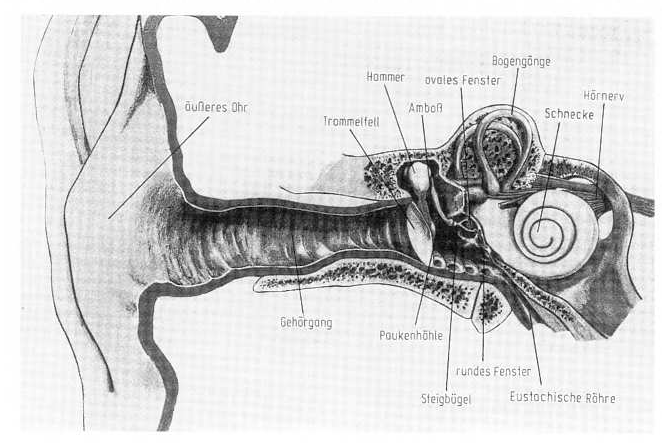
\includegraphics{Graph/ohr}
\caption[Schnitt durch das Geh�r]{Schnitt durch das Geh�r (aus \cite{handb_techak})} \label{fig:ohr}
\end{center}
\end{figure}

\subsection{Das Au�enohr}
Das \textbf{Au�enohr}\index{Au�enohr} ist das, was umgangssprachlich oft einfach nur als
Ohr bezeichnet wird, n�mlich die nach au�en \glqq sichtbaren\grqq$\:$  Teile unseres
Geh�rorgans. Es besteht aus der \textit{Ohrmuschel}, dem \textit{�u�eren Geh�rgang} und dem
\textit{Trommelfell}. Die Ohrmuschel stellt eine Art Schalltrichter da, die den Schall
auff�ngt und deren �bertragungsfunktion abh�ngig von der Einfallsrichtung des Schalls ist.
Der Schall gelangt dann �ber den $3-4cm$ langen Geh�rgang zum Trommelfell, einer Membran,
die durch den Schall zum Schwingen angeregt wird. Das Trommelfell stellt die Grenze zum
Mittelohr dar.
\subsection{Das Mittelohr}
Im \textbf{Mittelohr}\index{Mittelohr} befinden sich die Geh�rkn�chelchen \textit{Hammer,
Ambo�} und
\textit{Steig\-b�\-gel}, mit deren Hilfe die Schwingungen des Trommelfells auf eine weitere
Membran, das sogenannte \textit{ovale Fenster}, weitergeleitet werden. Der Hammer ist mit
dem Trommelfell verwachsen und ist durch ein Gelenk mit dem Ambo� verbunden, der wiederum
�ber ein Gelenk mit dem Steigb�gel verbunden ist.
\bem{Zwei kleine Muskeln setzen an Hammer bzw. Steigb�gel an. Auf sehr laute Ge\-r�usche reagieren diese mit einer Anspannung
und d�mpfen auf diese Weise allzu starke Bewegungen; sie �ben also eine gewisse
Schutzfunktion aus.}\end{quote}
\begin{sloppypar} Die Geh�rkn�chelchen wandeln Schwingungen
gro�er Amplitude und kleiner Kraft in solche kleiner Amplitude und gro�er Kraft um. Der
Steigb�gel �bertr�gt die gewandelten Schwingungen auf das \textit{ovale Fenster}, die
Grenze zum Innenohr.\\ Damit das Mittelohr seine Funktion gut erf�llen kann, mu� der
(statische) Druck innerhalb des Mittelohres dem Druck der Umwelt entsprechen. Der
Druckausgleich erfolgt �ber die \textit{Eustachische R�hre}, auch \textit{Ohrtrompete}
genannt.\end{sloppypar}
\bem{Die Eustachische R�hre verbindet das Mittelohr mit dem
Nasen-Rachen-Raum; aus diesem Grund l��t sich das unangenehme Druckgef�hl bei pl�tzlicher
�n\-derung des Au�endrucks, beispielsweise beim Starten eines Flugzeuges, durch Kauen oder
G�hnen beseitigen.}\end{quote}
\subsection{Das Innenohr}
Das \textbf{Innenohr}\index{Innenohr} enth�lt das Gleichgewichtsorgan und das eigentliche
H�rorgan, das die Form einer Schnecke hat und dementsprechend auch \textit{Schnecke} oder
\textit{Cochlea} hei�t. Die Schnecke ist im Gegensatz zum Mittelohr mit Fl�ssigkeit
gef�llt. Die Schnecke l��t sich in drei Kan�le aufteilen, welche  \textit{Scala vestibuli}
(Vorhoftreppe) , \textit{Scala media} und \textit{Scala tympani} (Paukentreppe) genannt
werden.
\begin{figure}[!hbt]
\begin{center}
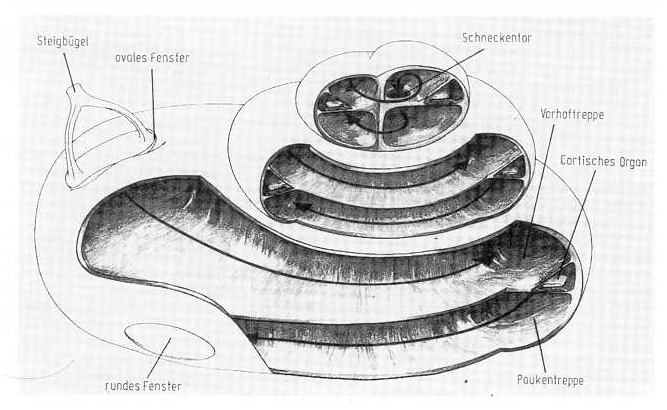
\includegraphics{Graph/cochleahbt}
\caption[Schnitt durch die Schnecke]{Schnitt durch die Schnecke (aus \cite{handb_techak})} \label{fig:cochleaschnitt}
\end{center}
\end{figure}

\begin{figure}[!hbt]
\begin{center}
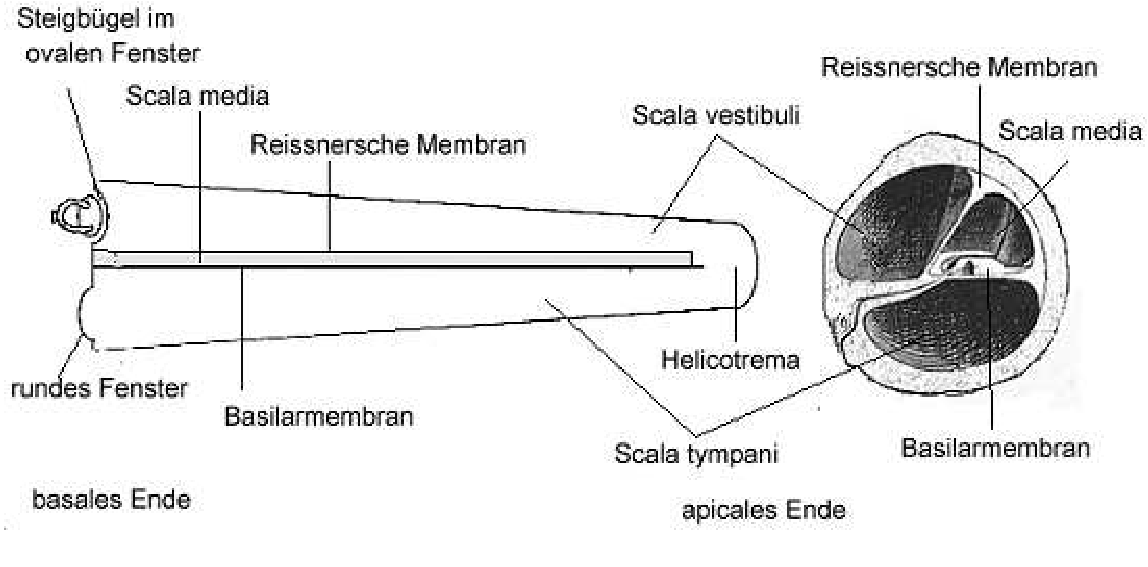
\includegraphics[scale=.5]{Graph/cochlea2}
\caption{Darstellung der Schnecke in abgerolltem Zustand} \label{fig:cochlea}
\end{center}
\end{figure}
\begin{sloppypar}
Die Schwingungen des Steigb�gels werden �ber das ovale Fenster auf die Fl�ssigkeit
�bertragen. Aufgrund der Druck�nderung in den Scalen wird die Basilarmembran, die sich
zwischen Scala media und Scala tympani befindet zum Schwingen angeregt. Auf dieser Membran
bilden sich Wanderwellen aus (s. Abb. \ref{fig:wanderw}). Dabei ist die Amplitude dieser
\begin{figure}[!hbt]
\begin{center}
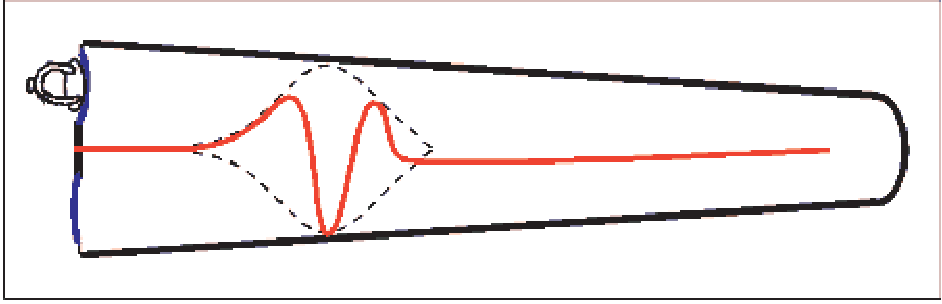
\includegraphics[scale=.5]{Graph/wanderw}
\caption{Wanderwelle auf der Basilarmembran} \label{fig:wanderw}
\end{center}
\end{figure}
Wanderwellen (bzw. die Einh�llende der Schwingung) abh�ngig von der anregenden Schwingung
und von der Position der Welle auf der Membran. Bei einer sinusf�rmigen Anregung steigt die
Amplitude zuerst langsam an, bis sie an einer bestimmten frequenzabh�ngigen Stelle ihr
Maximum erreicht und danach relativ schnell auf Null abklingt. Das bedeutet, da� sich auf
der Basilarmembran bestimmte Stellen auch bestimmten Frequenzen zuweisen lassen. T�ne hoher
Frequenz werden in der N�he des ovalen Fensters abgebildet, T�ne niedriger Frequenz in der
N�he des \textit{Schneckentors}.
\end{sloppypar}
\begin{figure}[!hbt]
\begin{center}
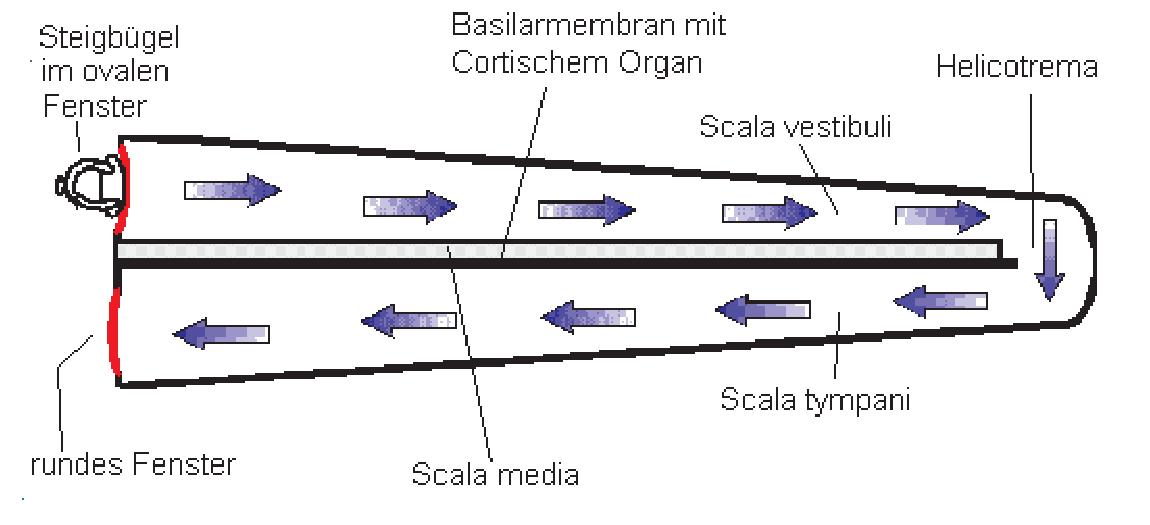
\includegraphics[scale=.5]{Graph/cochlea}
\caption{Fl�ssigkeitsstr�mung in der Schnecke} \label{fig:cochleastroem}
\end{center}
\end{figure}

Auf der Basilarmembran befindet sich das \textit{Cortische Organ}, welches die Aufgabe hat,
die Schwingungen in elektrische Impulsmuster umzusetzen. Das Cortische Organ besitzt eine
Vielzahl von Sinneszellen\footnote{Die Anzahl ist ca. 14000.}, auch Haarzellen genannt,
welche die Schwingungsform der Basilarmembran abtasten. Die Haarzellen in der Umgebung der
Maximalamplitude der Wanderwelle werden am st�rksten angeregt; da jede Haarzelle von
Einzelfasern des H�rnervs kontaktiert wird, kann das Geh�r eine Tonh�he zuordnen. Die
Codierung der Reizintensit�t geschieht durch die Frequenz, mit der die Neuronen feuern. Mit
zunehmendem Schalldruck nimmt also auch die Impulsfrequenz der Nervenzellen im Innenohr zu.

\section{Schalldruckpegel, Lautst�rke und Lautheit}\label{chap:lautstaerke}
Die empfundene Lautst�rke eines Schallereignisses ist nicht nur abh�ngig von dem
Schalldruckpegel, sondern auch von dessen Frequenzzusammensetzung. Beispielsweise rufen
zwei Sinust�ne unterschiedlicher Frequenz aber gleichen Pegels im allgemeinen eine
unterschiedliche Lautst�rkeempfindung hervor. Dieser Sachverhalt wird verdeutlicht durch
die sogenannten \textbf{Kurven gleicher Lautst�rkepegel}\index{Kurven gleicher
Lautst�rkepegel} (s. Abb. \ref{fig:kurvengls}).
\begin{figure}[!hbt]
\begin{center}
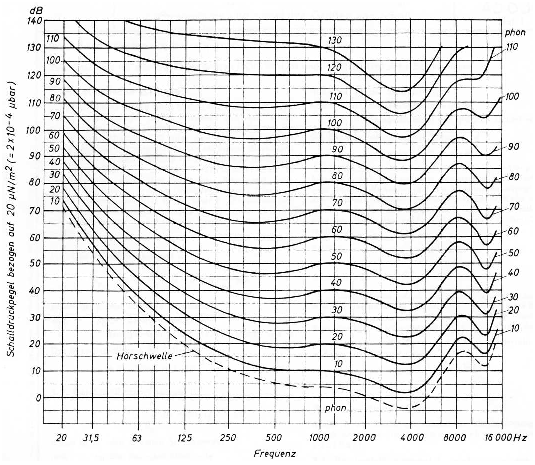
\includegraphics{Graph/Kurvengl}
\caption[Normalkurven gleicher Lautst�rkepegel]{Normalkurven gleicher Lautst�rkepegel (aus DIN 45 630)}
\label{fig:kurvengls}
\end{center}
\end{figure}
Hier erkennt man, da� der Schalldruckpegel f�r unterschiedliche Frequenzen sich teilweise
stark ver�ndern mu�, um das gleiche Lautst�rkeempfinden hervorzurufen. Die Einheit
\textit{phon}\index{phon} versucht, das Lautst�rkeempfinden nachzubilden. Eine einzelne Kurve der Kurven gleicher Lautst�rkepegel hat einen festen $phon$-Wert. So wird beispielsweise ein
Ton beliebiger Frequenz mit der Lautst�rke $80 phon$ als gleichlaut mit einem Sinuston der
Frequenz $1kH\!z$ mit dem Schalldruckpegel $80dB$ empfunden. Besonders im Bereich zwischen
$2$ und $5kH\!z$ ist das Ohr sehr empfindlich.\\ Die Kurven gleicher Lautst�rkepegel
verlaufen nicht parallel zueinander, sondern haben f�r unterschiedliche Lautst�rken auch
einen leicht unterschiedlichen Verlauf. Insbesondere wird ein leiser wiedergegebenes
Schallereignis ba�- und auch leicht h�hen�rmer erscheinen als ein lautes.
\bem{F�r Aufnahme und Mischung kann dieses Wissen
von Bedeutung sein. Ein wichtiger Anhaltspunkt ist, wie laut die Mischung sp�ter
erwartungsgem�� abgeh�rt wird, ob die Abh�rlautst�rke bei der Mischung dar�ber oder
darunter liegt und wie sich das auf die wahrgenommene Frequenzverteilung auswirkt. Ein
Probeh�ren der Mischung in anderen Lautst�rken kann hilfreich sein.}\end{quote} Die
\textbf{Lautheit}\index{Lautheit} wird in der Einheit \textit{sone}\index{sone} angegeben. Als Bezugswert wurde dem
Wert $1 sone$ ein Sinuston der Frequenz $1kH\!z$ und dem Schalldruckpegel $40dB$ zugeordnet.
Ein doppelt so laut empfundener Schallvorgang hat die Lautheit $2 sone$ (was $+10phon$
entspricht), ein vierfach so laut empfundener $4 sone$. 
\bem{Im Tonstudioalltag wird man sich mit der Einheit \textit{sone} i.a. nicht besch�ftigen m�ssen. In der akustischen Me�technik spielt sie allerdings eine Rolle; z.B. wird in Qualit�tstests von Computerfestplatten oft der St�rschall in $sone$ angegeben.}\end{quote}
 Die Kurven gleicher
Lautst�rke betrachten nur den pegelabh�ngigen Frequenzgang des Ohres. Auch andere Parameter
k�nnen aber das Lautst�rkeempfinden beeinflussen. So wirkt beispielsweise eine sehr kurzes
Schallsignal leiser als das gleiche Signal gleichen Pegels l�nger ausgehalten.
\chaplink
\begin{itemize}
	\item Abschnitt \ref{chap:amplitude}
	\item Abschnitt \ref{chap:ss-pegel}
\end{itemize}
\end{quote}

\section{Tonh�henempfindung}\label{chap:pitch}
Die Tonh�henempfindung ist nicht ausschlie�lich abh�ngig von der Frequenz (wie in
\ref{chap:freq} beschrieben), sondern auch von der Lautst�rke eines Tones. Bei Frequenzen
�ber zweitausend Hertz steigt die empfundene Tonh�he mit zunehmendem Pegel leicht an
w�hrend sie bei Frequenzen unter $1kH\!z$ mit zunehmenden Pegel leicht abf�llt. Zur
weitergehenden Vertiefung sei auf \cite{zwicker} und \cite{verschuure} verwiesen.
\chaplink
\begin{itemize}
	\item Abschnitt \ref{chap:freq}
	\item Abschnitt \ref{chap:webfech}
\end{itemize}
\end{quote}

\section{Verdeckungseffekte}\label{chap:masking}
Es lassen sich nicht immer alle Informationen wahrnehmen, die in einem Musiksignal
enthalten sind. Vielmehr treten in bestimmten F�llen sogenannte
\textbf{Verdeckungseffekte}\index{Verdeckungseffekte} auf. So verdeckt beispielsweise ein
einzelner Sinuston dicht neben dieser Frequenz liegende Signalanteile (s.
Abb. \ref{fig:spreading}); diese sind unh�rbar.
\begin{figure}[!hbt]
\begin{center}
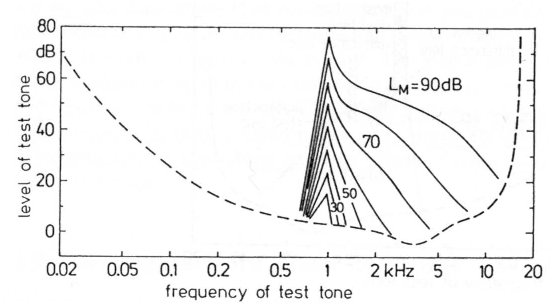
\includegraphics{Graph/spread}
\caption[Mith�rschwelle eines Sinustones]{Pegel eines Sinustons, der von einem $1kH\!z$-Sinuston unterschiedlichen Pegels maskiert wird, als Funktion der Frequenz des Testtones (aus \cite{zwicker})}
\label{fig:spreading}
\end{center}
\end{figure}

Neben den Verdeckungseffekten im Frequenzbereich gibt es auch noch zeitliche
Verdeckungseffekte, n�mlich die \textbf{Nachverdeckung}\index{Nachverdeckung} (auch \emp{Forward Masking} oder \emp{Postmasking}) und die
\textbf{Vorverdeckung}\index{Vorverdeckung}auch \emp{Backward Masking} oder \emp{Premasking}). In Abb. \ref{fig:masking} sind die Auswirkungen dieser Effekte dargestellt. Es gibt also kurz vor und
kurz nach einem Signal eine Zeit, in welcher wir unter einer gewissen Schwelle liegenden
Schallereignisse nicht mehr wahrnehmen k�nnen.
\begin{figure}[!hbt]
\begin{center}
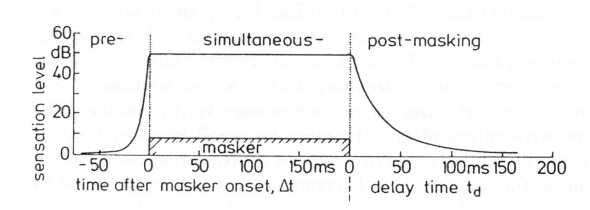
\includegraphics{Graph/masking}
\caption[Pre- und Postmasking]{Bereiche, in denen Pre- und Postmasking auftritt (aus \cite{zwicker})}
\label{fig:masking}
\end{center}
\end{figure}

\bem{Bei der verlustbehafteten Codierung von Audiosignalen (z.B. die MPEG-Formate, Dolby AC-3, Sony ATRAC, etc.) wird versucht,
diese Eigenschaften des Geh�rs bzw. der Wahrnehmung auszunutzen und solche Signalanteile,
die i.a. nicht mehr wahrgenommen werden k�nnen, gleich \glqq wegzulassen\grqq$\:$ .}\end{quote}
	\ifthenelse{\equal{\value{allchaps}}{1}}
{
\chaplink
\begin{itemize}
	\item Abschnitt \ref{chap:codecs}
\end{itemize}
\end{quote}
}{}

\section{Richtungsh�ren bei einer Schallquelle}\label{chap:local}
Viele Untersuchungen haben sich mit der Richtungslokalisation von Schallquellen
besch�ftigt. Die wahrzunehmende Aufl�sung in Blickrichtung
(\textbf{Lokalisations\-sch�rfe}\index{Lokalisationssch�rfe}) ist abh�ngig von
Versuchsaufbau und verwendetem Tonsignal. Um diese Abh�ngigkeit zu veranschaulichen, sind
in der Tabelle \ref{tab:lokalisation} die Ergebnisse einiger Testreihen mit
unterschiedlichen Schallquellen aufgef�hrt.\\
\begin{table}[h]
\begin{footnotesize}
\begin{center}
\begin{tabular}{|l|l|l|}\hline
\textbf{Ver�ffentlichung}&\textbf{Art des Signals}&\textbf{Lokalisationssch�rfe}\\\hline
         Klemm (1920)         &                        Impulses (clicks)                         &  0.75�-2�  \\\hline
    King and Laird (1930)     &                      Impulse (click) train                       &    1.6�    \\\hline
  Stevens and Newman (1936)   &                            Sinusoids                             &    4.4�    \\\hline
    Schmidt et al. (1953)     &                            Sinusoids                             &    >1�     \\\hline
     Sandel et al. (1955)     &                            Sinusoids                             & 1.1�-4.0�  \\\hline
         Mills (1958)         &                            Sinusoids                             & 1.0�-3.1�  \\\hline
        Stiller (1960)        &               Narrow-band noise, $cos^2$ tone bursts             & 1.4�-2.8�  \\\hline
       Boerger (1965a)        &                       Gaussian tone bursts                       & 0.8�-3.3�  \\\hline
       Gardner (1968a)        &                              Speech                              &    0.9�    \\\hline
        Perrott (1969)        & Tone bursts                                                      & 1.8�-11.8� \\\hline
       Blauert (1970b)        &                              Speech                              &    1.5�    \\\hline
 Haustein and Schirmer (1970) &                          Broadband noise                         &    3.2�    \\\hline
\end{tabular}
\end{center}
\end{footnotesize}
\caption[Lokalisationssch�rfe bei horizontaler Verschiebung der Schallquelle]{unterschiedliche Messungen zur Lokalisationssch�rfe bei horizontaler Verschiebung
der Schallquelle aus der Blickrichtung (aus \cite{blauert})} \label{tab:lokalisation}
\end{table}
Die Lokalisation einer Schallquelle wird vor allem durch das beidohrige
(\textit{binaurale})\index{binaural} H�ren erm�glicht. Vom Gehirn werden die
(\textit{interauralen}) Unterschiede zwischen den Schallsignalen am linken und am rechten
Ohr ausgewertet und die Richtung der Schallquelle bestimmt. Ma�gebliche Parameter der
Richtungslokalisation sind
\textit{Laufzeitunterschiede} und
\textit{Pegelunterschiede} zwischen den Ohren. Wie Abb. \ref{fig:ortung} schematisch
veranschaulicht, gelangt ein Schallsignal im allgemeinen nicht gleichzeitig an beide Ohren,
sondern wird an dem der Schallquelle zugewandten Ohr
\begin{figure}[!hbt]
\begin{center}
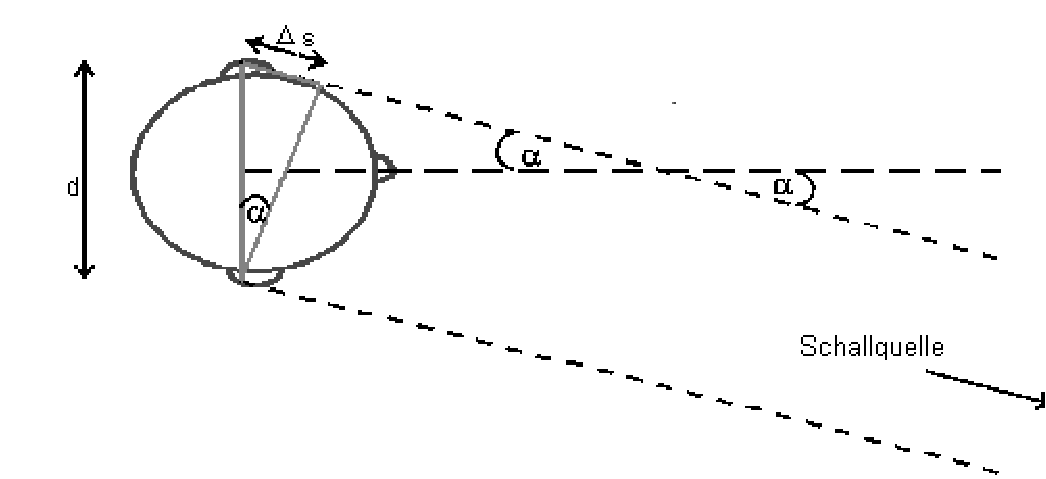
\includegraphics[scale=.5]{Graph/ortung1}
\caption{Laufzeitunterschiede zwischen beiden Ohren f�r eine
Schallquelle}\label{fig:ortung}
\end{center}
\end{figure}
fr�her eintreffen. Auch gelangt durch die Abschattung des Kopfes das Schallsignal
frequenzabh�ngig mit geringerem Pegel an das der Schallquelle abgewandte Ohr.
\bem{Diese
D�mpfung ist frequenzabh�ngig; hohe Frequenzen werden st�rker ged�mpft als tiefe (s.
Abschnitt
\ref{chap:beugung}).}\end{quote} Zus�tzlich zu der Auswertung der Signalunterschiede
zwischen beiden Ohren gibt es auch noch die �bertragungsfunktion unserer Au�enohren. Durch
diese wird es erm�glicht, zum Beispiel zwischen vorne und hinten zu unterscheiden, was ja
anhand von Signalunterschieden nicht m�glich w�re\footnote{Allein aufgrund der
�bertragungsfunktion des Au�enohres ist das noch nicht ausreichend gut m�glich; zus�tzlich
zu den Au�enohr�bertragungsfunktionen werden vom H�rer auch sehr geringe Kopfbewegungen
ausgef�hrt, um durch die dadurch auftretenden Laufzeit- und Pegeldifferenzen zwischen den
m�glichen Einfallsrichtungen zu unterscheiden}. Der Einflu� der Au�enohren auf den \glqq
geh�rten\grqq$\:$  Frequenzgang des eintreffenden Schalls ist abh�ngig von der Einfallsrichtung
und ist bei jedem Menschen leicht unterschiedlich. Es lassen sich aber einige typische
Frequenzen angeben, die f�r einen bestimmten Richtungseindruck stehen.
Abb. \ref{fig:baender} zeigt Untersuchungsergebnisse, welche verdeutlichen, da� der
Richtungseindruck stark von der
\begin{figure}[!hbt]
\begin{center}
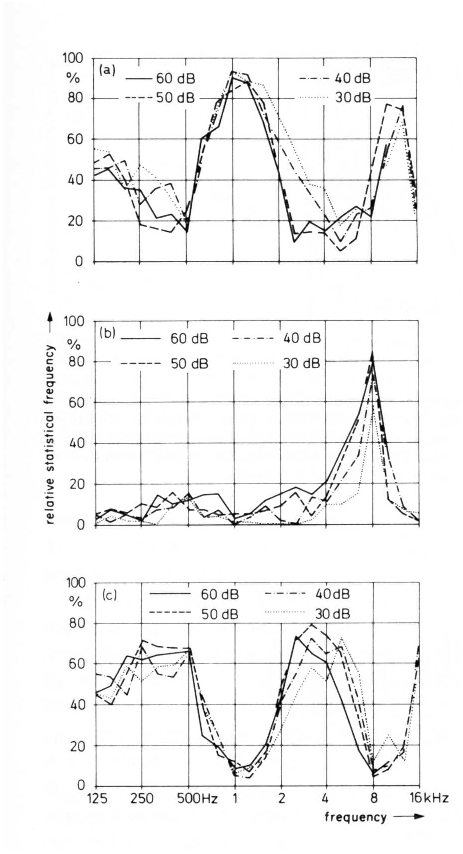
\includegraphics[scale=.8]{Graph/baender}
\caption[Richtungseindruck aufgrund der Signalfrequenz]{relative H�ufigkeit der Antworten \textit{hinten}, \textit{oben}, \textit{vorne}
�ber der Mittenfrequenz eines Terzbandrauschens (einmal von vorne und einmal von hinten
eingespielt) aufgetragen (aus \cite{blauert})} \label{fig:baender}
\end{center}
\end{figure}
Frequenz eines Signals abh�ngt.  Hier wurde zur Messung Terzbandrauschen mit
unterschiedlicher L�nge verwendet. Man erkennt beispielsweise, da� bei einer Mittenfrequenz
von $1kH\!z$ ca. 90 Prozent der Testpersonen das Signal hinter sich orten, w�hrend das
Schallereignis bei einer Mittenfrequenz von $8kH\!z$ oben lokalisiert wird. Sind Frequenzen
um $4kH\!z$ in einem Signal enthalten, so erh�ht sich der \glqq Vorne-Eindruck\grqq, die
Pr�senz eines Signals. Diese Frequenzbereiche werden
\textbf{richtungsbestimmende B�nder}\index{richtungsbestimmende B�nder} genannt. Das Wissen
um die Wirkung dieser verschiedenen Frequenzb�nder kann beim Filtern durchaus hilfreich
sein, da man schon einen Anhaltspunkt hat, in welchem Frequenzbereich man zun�chst suchen
sollte, um den gew�nschten Effekt zu erzielen.
\begin{figure}[!hbt]
\begin{center}
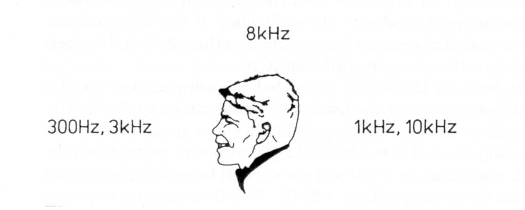
\includegraphics{Graph/baender2}
\caption[richtungsbestimmende B�nder in der Medianebene]{Veranschaulichung der richtungsbestimmenden B�nder in der Medianebene, unabh�ngig
von der Position der Quelle (aus \cite{zwicker})} \label{fig:baender2}
\end{center}
\end{figure}
	\ifthenelse{\equal{\value{allchaps}}{1}}
{
\chaplink
\begin{itemize}
	\item Abschnitt \ref{chap:filter}
\end{itemize}
\end{quote}
}{}

\subsection{Das Gesetz der ersten Wellenfront}\label{chap:firstfront}
Zwei �hnliche Signale, die aus unterschiedlichen Richtungen kommen (z.B. Direktschall und
ein R�ckwurf), werden aus der Einfallsrichtung lokalisiert, aus welcher die erste
Wellenfront eintrifft. Dieser Sachverhalt wird \textbf{Gesetz der ersten
Wellenfront}\index{Gesetz!der ersten Wellenfront} bzw.
\textbf{Prezedenzeffekt}\index{Prezedenzeffekt} genannt. Die Verz�gerung des zweiten Signals darf allerdings eine
gewisse Schwelle (\textit{Echoschwelle}\index{Echoschwelle}) nicht �berschreiten, da der
H�rer in einem solchen Fall zwei einzelne Signale (z.B. Direktschall und Echo) wahrnimmt.
Die \textit{Echoschwelle} ist abh�ngig von der Verz�gerungszeit und dem Pegel des zweiten
Signals (s. Abb. \ref{fig:echoschwelle}). Ist die Verz�gerung des zweiten Signals sehr
klein, so entsteht ein anderes Ph�nomen, die Summenlokalisation (s. Abschnitt
\ref{chap:richt_stereo}.
	\begin{figure}[!hbt]
		\begin{center}
			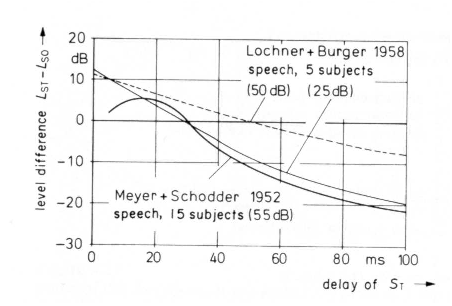
\includegraphics{Graph/echo}
			\caption[Echoschwelle bei Sprache]{Verschiedene Messungen zur Echoschwelle bei Sprache (aus \cite{blauert})}
			\label{fig:echoschwelle}
		\end{center}
	\end{figure}
Versucht man bei zwei identischen Signalen, die durch allm�hliche Verz�gerung des zweiten
Signals verschobene Richtungswahrnehmung wiederum durch Pegelerh�hung des zweiten Signals
auszugleichen, was \textit{Trading}\index{Trading} genannt wird, so erh�lt man die in
Abb. \ref{fig:laufzeit-pegel} dargestellte Funktion.
	\begin{figure}[!hbt]
		\begin{center}
			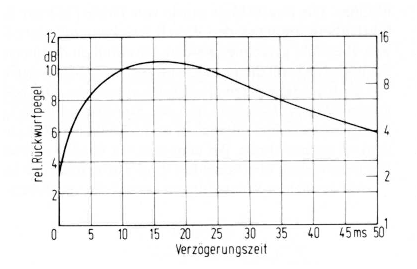
\includegraphics{Graph/laufpeg}
			\caption[Tradingeffekt]{Pegel eines R�ckwurfes, bei dem die Richtungslokalisation des Direktschalls
			zerst�rt wird (aus \cite{handb_techak})} \label{fig:laufzeit-pegel}
		\end{center}
	\end{figure}
Man k�nnte also ein um $15ms$ verz�gertes Signal um bis zu $10dB$ anheben, ohne da� dieses
Signal als einzelnes wahrzunehmen w�re. Diese Messung erfolgte allerdings mit
Sprachsignalen, l��t sich also demnach nur n�herungsweise auf Musik �bertragen.
\bem{Bei Beschallungen mit mehreren Lautsprechersystemen wird oft mit entsprechenden
Verz�gerungen gearbeitet, um den Pegel des zu verst�rkenden Signals erh�hen zu k�nnen, ohne
die Ortbarkeit des Direktsignals zu verlieren.}\end{quote}
	\ifthenelse{\equal{\value{allchaps}}{1}}
{
\chaplink
\begin{itemize}
	\item Abschnitt \ref{chap:delay}
\end{itemize}
\end{quote}
}{}

\section{Richtungsh�ren im Stereodreieck}\label{chap:richt_stereo}
Gibt man im Stereodreieck (Abb. \ref{fig:stereodreieck}) auf die Lautsprecher korrelierte
Signale gleichen Pegels, so ortet man die Schallquelle auf der Lautsprecherbasis, also in
der Mitte.
	\begin{figure}[!hbt]
		\begin{center}
			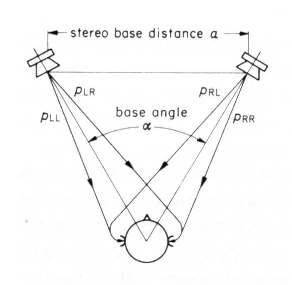
\includegraphics{Graph/sterdrei}
			\caption[�bliche Lautsprecher-Stereoaufstellung]{�bliche Lautsprecher-Stereoaufstellung, der Winkel $\alpha$ zwischen den beiden Lautsprechern betr�gt normalerweise ca. $60^\circ $ (aus \cite{blauert})}
			\label{fig:stereodreieck}
		\end{center}
	\end{figure}
Eine solche virtuelle Schallquelle hei�t \textbf{Phantomschallquelle}\index{Phantomschallquelle}\footnote{siehe in der einschl�gigen Literatur unter \textit{Summenlokalisation} und \textit{Assoziationsmodell von Theile.}}. Um die Phantomschallquelle aus der Mitte heraus zu bewegen, kann man Pegel- und/oder Laufzeitdifferenzen benutzen. Bei welchen Pegel- bzw. Laufzeitunterschieden zwischen den Signalen \textit{links} und \textit{rechts} verschiebt sich nun die Ortung einer Phantomschallquelle im klassischen Stereo-Panorama (s. Abb. \ref{fig:stereodreieck})? Abb. \ref{fig:phantom} und Abb. \ref{fig:phantomfreq} veranschaulichen, wie weit sich die Ortung der Phantomschallquelle bei �nderung des Pegelunterschiedes oder der Verz�gerung zwischen \textit{links} und \textit{rechts} aus der Mitte verschiebt.
\begin{figure}[!hbt]
\begin{center}
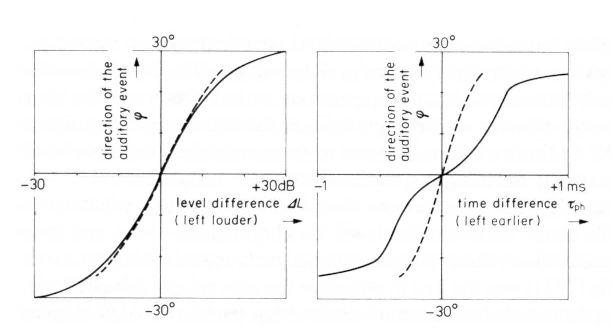
\includegraphics{Graph/richt}
\caption[Lokalisation einer Phantomschallquelle (Sprache)]{Lokalisation einer Phantomschallquelle im Stereodreieck (nach
Abb. \ref{fig:stereodreieck}); links Pegelunterschiede, rechts Laufzeitunterschiede; Signal
Sprache, gestrichelte Linien f�r bewegbaren Kopf, durchgezogene Kurven f�r feststehenden
Kopf (aus \cite{blauert})} \label{fig:phantom}
\end{center}
\end{figure}
\begin{figure}[!hbt]
\begin{center}
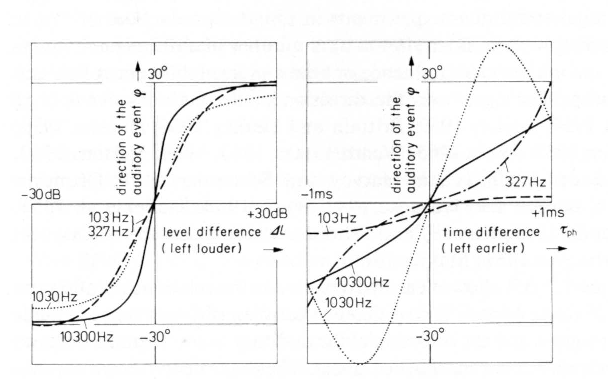
\includegraphics{Graph/richtfreq}
\caption[Lokalisation einer Phantomschallquelle (Sinusburst)]{Lokalisation einer Phantomschallquelle im Stereodreieck nach
Abb. \ref{fig:stereodreieck}; links Pegelunterschiede, rechts Laufzeitunterschiede; Signal
terzbreite Sinusbursts verschiedener Frequenzen, gestrichelte Linien f�r bewegbaren Kopf,
durchgezogene Kurven f�r feststehenden Kopf (aus \cite{blauert})} \label{fig:phantomfreq}
\end{center}
\end{figure}
Auch bei den Abb. \ref{fig:phantom} und \ref{fig:phantomfreq} wird wiederum deutlich, wie
stark die Messungen von dem Testsignal abh�ngen. Eine generelle Aussage, z.B. ab welchem
Laufzeitunterschied oder welcher Pegeldifferenz ein Signal in einem Lautsprecher geortet
wird, ist nur sehr grob m�glich.

\section{Zusammenfassung}
Das Ohr l��t sich in drei Teile untergliedern: \textbf{Au�enohr}, \textbf{Mittelohr} und
\textbf{Innenohr}. Der Schall gelangt �ber den Geh�rgang zum \textit{Trommelfell} und
versetzt dieses in Schwingung. Die \textit{Geh�rkn�chelchen} im Mittelohr �bertragen die
Schwingungen des Trommelfells auf das \textit{ovale Fenster}, die Grenze zum Innenohr. Im
Innenohr befindet sich die Schnecke, das eigentliche H�rorgan. Hier werden die Schwingungen
auf die \textit{Basilarmembran} �bertragen, deren Schwingungen dann die
\textit{Haarzellen}, Nerven auf der Basilarmembran, zum Feuern anregen.\\ Die
\textbf{Lautst�rke}, mit der wir ein Schallereignis empfinden, l��t sich nur n�he\-rungs\-weise
mit dem absoluten Schalldruckpegel beschreiben. Tats�chlich ist das Lautst�rkeempfinden
sehr stark abh�ngig von der Art des Schallereignisses, sowohl von dessen zeitlicher als
auch frequenzm��iger Zusammensetzung. Die \textbf{Kurven gleicher Lautst�rkepegel} zeigen
das frequenzabh�ngige Lautst�rke\-empfin\-den. Einheiten, die dieses Empfinden nachvollziehen,
sind beispielsweise \textit{phon} und \textit{sone}.\\ Nicht alle in einem Audiosignal
enthaltenen Informationen m�ssen wirklich h�rbar sein. Es gibt
\textbf{Verdeckungseffekte}, bei denen ein bestimmtes Schallereignis andere Ereignisse unh�rbar macht. Diese Effekte existieren sowohl im Zeit- als auch im Frequenzbereich.
\\Der Mensch kann eine Schallquelle v.a. aufgrund der \textit{Laufzeit}- und
\textit{Pegelunterschiede} zwischen beiden Ohren im Raum lokalisieren. Eine etwas untergeordnete Rolle
spielen f�r die Ortung auch die \textit{Au�enohr�bertragungsfunktionen}. Alle drei
Parameter der Lokalisation lassen sich auch zusammenfassen in den sogenannten kopfbezogenen
�bertragungsfunktionen (HRTF: \textit{H}ead \textit{R}elated \textit{T}ransfer
\textit{F}unctions).\\ Der \textbf{Prezedenzeffekt} bzw. das \textbf{Gesetz der ersten
Wellenfront} besagt, da� Schall aus der Richtung lokalisiert wird, aus der die erste
Wellenfront beim H�rer eintrifft.\\ Im Stereodreieck hat man zwei Schallquellen (die
Lautsprecher). Liegen auf beiden Lautsprechern korrelierte Signale, so bildet sich eine
\textbf{Phantomschallquelle} zwischen den beiden Lautsprechern. Durch Laufzeit- und/oder
Pegeldifferenzen zwischen den beiden Lautsprechersignalen l��t sich die Phantomschallquelle
zwischen den beiden Lautsprechern bewegen. Abh�ngig vom Signal sind Pegeldifferenzen
zwischen $15$ und $20dB$ bzw. Laufzeitunterschiede zwischen $0.7$ und $1ms$, u.U. bis zu
$2ms$ notwendig, um die Phantomschallquelle ganz in einen Lautsprecher zu verschieben.
Diese Werte sind nicht zu verwechseln mit den \textit{interauralen} Laufzeit- und
Pegeldifferenzen, die wesentlich kleiner sind.



\section{Aufgaben}
\begin{enumerate}
	\item	Zwei parallel ausgerichtete Mikrophone stehen im Abstand von $50cm$. Im Abstand von $5m$ zu der gedachten Vebindungslinie zwischen den Mikrophonen befindet sich eine Schallquelle, die aber um $25cm$ aus der Mitte verschoben ist, so da� Mikrophone und Quelle ein rechtwinkliges Dreieck bilden. Wie gro� sind die Pegel- und Laufzeitunterschiede zwischen den Mikrophonen?
	
	\item	Wie weit m��te man das weiter entfernte Mikrophon verschieben, um eine Laufzeitdifferenz von $1ms$ zu erreichen?
	
	\item Wie gro� kann der Lautzeitunterschied zwischen den beiden Ohren maximal sein, wenn das Signal komplett um den Kopf herum gebeugt wird? Der Kopf soll dabei durch eine Kugel mit Radius $10cm$ angen�hert werden, die Schallgeschwindigkeit sei $340\frac{m}{s}$.
\end{enumerate}

\nocite{moore, stevens}
% m�gliche Ger�te: EQ, Pan; Aufgaben: -> Grundlagen der Mikrophonaufstellung
	\ifthenelse{\equal{\value{allchaps}}{1}}
	{
	%\chapter{Musikalische Akustik}\label{chap:musak}
\thispagestyle{empty}
\section{Stimmungen}
\section{Charakteristische Klangmerkmale}

\section{Streichinstrumente}
\subsection{Klangentstehung}
\subsection{Klangabstrahlung}

\section{Zupfinstrumente}
\subsection{Klangentstehung}
\subsection{Klangabstrahlung}

\section{Schlaginstrumente}
\subsection{Klangentstehung}
\subsection{Klangabstrahlung}

\section{elektronische Instrumente}
\subsection{Klangentstehung}
\subsection{Klangabstrahlung}

\section{Zusammenfassung}

\section{Aufgaben}

\nocite{meyer}
% 
	%\chapter{Elektrotechnik}
\thispagestyle{empty}

\section{Spannung und Strom}

\section{symm. und unsymm. �bertragung}

\section{Anpassung}

\section{�bertrager}

\section{Zusammenfassung}

\section{Aufgaben}
%
	\chapter{Signalverarbeitung}
\thispagestyle{empty}

Dieses Kapitel stellt eine Einf�hrung in die wichtigsten Begriffe der Signalverarbeitung dar. Zun�chst geht es relativ theoretisch um Systembeschreibungen, anschlie�end geht es um einen kurzen �berblick �ber verschiedene Effekte und Qualit�tsmerkmale.

\section{Signalbeschreibungen}\label{chap:sigbesch}
Nachdem in vorherigen Abschnitten wiederholt sowohl Darstellungen des Zeitverlaufs wie auch Frequendarstellungen von Signalen auftauchten, soll dieses Kapitel diese Darstellungen nun detaillierter erkl�ren.
\subsection{Zeitverlauf}\index{Zeitdarstellung}\label{chap:timedesc}
Der \bld{Zeitverlauf} eines Signals ist die gel�ufigste und am einfachsten verst�ndliche Darstellung eines Audiosignals. Nimmt man z.B. den Schalldruck eines akustischen Ereignisses an einem Ort auf, und zeichnet die Druckschwankungen �ber der Zeit auf, so betrachtet man den Zeitverlauf des Drucks. Dabei nimmt die Zeit nach rechts hin zu, und die Amplitude des Drucks wird nach oben aufgetragen. Nichts anderes ist auch die Wellenformdarstellung unterschiedlichster Audiobearbeitungsprogramme, wo die �nderungen der Amplitude des Signals �ber der Zeit dargestellt werden. Abb. \ref{fig:timeplot} zeigt beispielhaft die Zeitdarstellung eines Audiosignals.
    \begin{figure}[!hbt]
			\begin{center}
			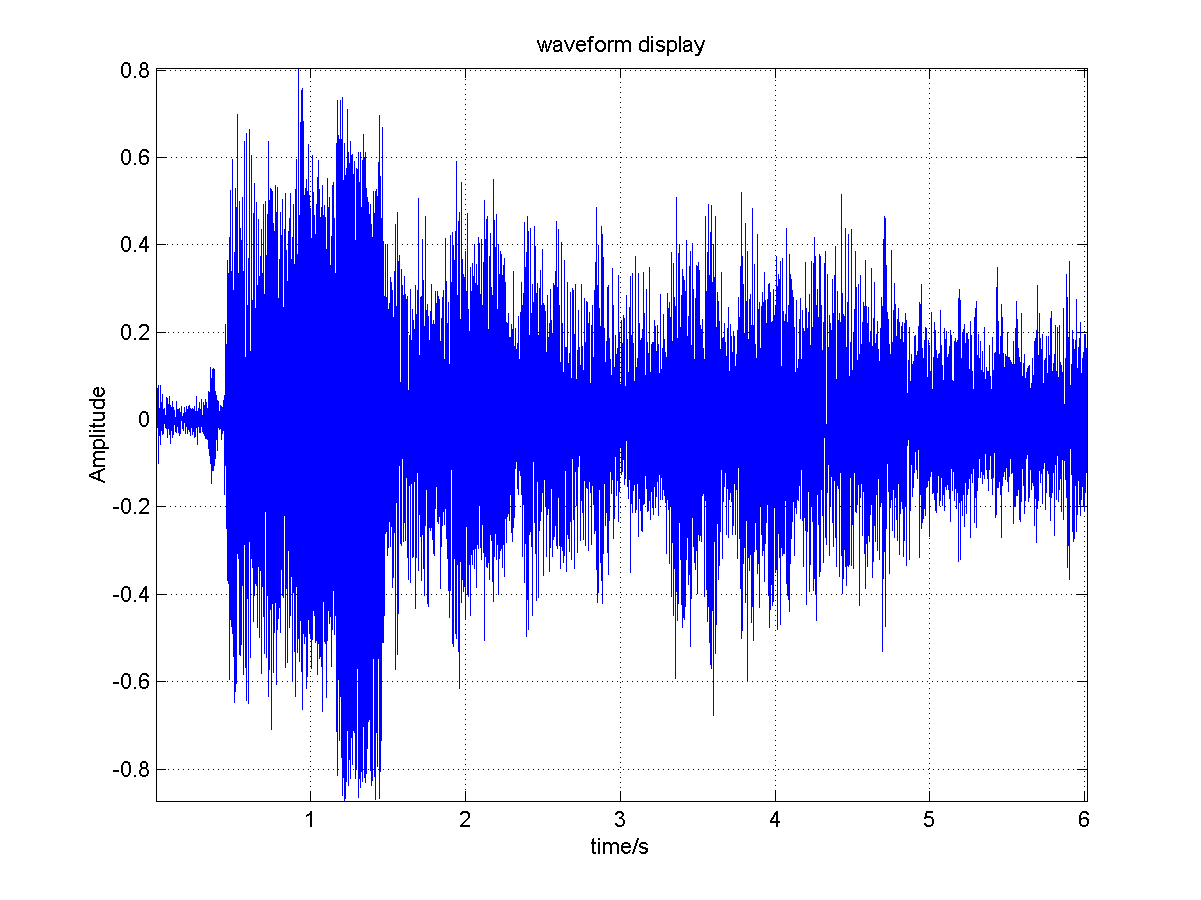
\includegraphics[scale=0.5]{Graph/timesignal}
			\caption[Zeitdarstellung eines Audiosignals]{Zeitdarstellung eines Audiosignals; diese Beispiel ist ein kurzer Ausschnitt aus einem St�ck mit der Besetzung Gesang und Klavier} \label{fig:timeplot}
			\end{center}
		\end{figure}

\subsection{Spektrum}\index{Spektrum}\index{Frequenzdarstellung}\index{Fouriertransformation}\label{chap:spectrumdesc}
Ebenso wie mit der Zeitdarstellung eines Signals, wurde auch schon mit seiner \bld{Frequenzdarstellung}, dem Spektrum eines Signals in vorhergehenden Kapiteln gearbeitet. Beispielsweise zeigt die Abb. \ref{fig:schwingadd} links den Zeitverlauf und rechts das Frequenzspektrum von Sinusschwingungen. Je h�her die Frequenz einer Schwingung ist, desto mehr rutscht der Peak dieser Schwingung auf der Frequenzachse nach rechts. Sinusf�rmige Schwingungen besitzen nur einen einzigen Frequenzanteil; in realen Signalen k�nnen dagegen sehr viele Frequenzen zur gleichen Zeit auftreten. Die Frequenzdarstellung wird auch Fouriertransormation des Signals genannt. Da Musiksignale sich auch �ber die Zeit st�ndig �ndern, kann man allerdings aus Langzeitspektren kaum interessante Informationen sehen. Aus diesem Grund werden selten Frequenzanalysen eines kompletten l�ngeren Signalabschnitts gemacht. Eine wichtige Eigenschaft der Fouriertransformation ist, da� die Transformation in beide Richtungen m�glich ist, d.h. jedes Spektrum l��t sich genauso leicht in den Zeitverlauf umrechnen wie andersherum.\\
F�hrt man eine Spektralanalyse (eines digitalen Signals) �ber N Samples durch, so erh�lt man genau $N/2$ komplexe Spektralwerte, die gleichf�rmig �ber das Spektrum verteilt sind. Nimmt man beispielsweise $1024$ Signalwerte eines Signals der Abtastfrequenz $48k\!Hz$, so hat man eine zeitliche Aufl�sung von $21.3ms$ und eine Frequenzaufl�sung von $46.9H\!z$. Je gr�ber also die zeitliche Aufl�sung wird, desto feiner wird die Frequenzaufl�sung und umgekehrt. Dies ist wichtig, denn das Signal sollte in sich innerhalb eines Analysefensters nicht zu sehr �ndern. Abb. \ref{fig:spektrum} zeigt die verschiedene Darstellungsm�glichkeiten der komplexen Werte des schon in Abb. \ref{fig:timeplot} verwendeten Signals. Dieses Signal ist eigentlich schon viel zu lang, um eine Frequenzanalyse davon durchzuf�hren, aus diesem Grund ist das Ergebnis auch nicht sonderlich interessant zu betrachten. Abb. \ref{fig:dbSpektrum} ist die gel�ufige Darstellungsweise eines Signalspektrum; hier wir der Betragsfrequenzgang in Dezibel gezeigt. Da der Signalausschnitt jedoch f�r eine FFT-Analyse eigentlich zu lang ist, gibt es noch weitere Darstellungsm�glichkeiten, in der Zeit- und Frequenzverlauf in gewisser Hinsicht vereint werden, z.B. das sogenannte Spektrogramm\index{Spektrogramm}, das in Abb. \ref{fig:specgram} dargestellt ist, oder eine Pseudo-3D-Grafik wie in Abb.\ref{fig:3dsignal}.
    \begin{figure}[!hbt]
			\begin{center}
			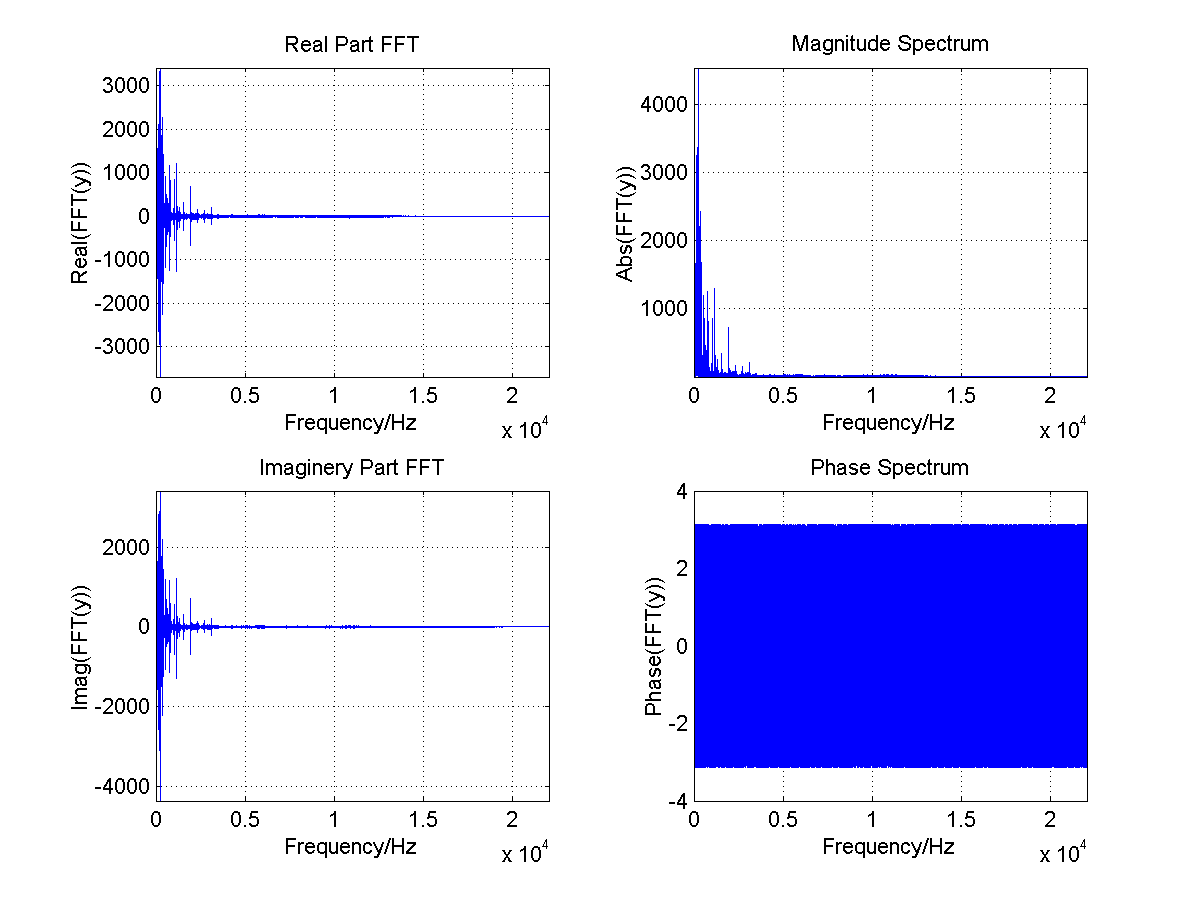
\includegraphics[scale=0.5]{Graph/fftsignal}
			\caption[FFT eines Audiosignals]{Frequenzspektrum eines Audiosignals, links als Real- und Imagin�rteil, rechts mit Betrag- und Phasenspektrum} \label{fig:spektrum}
			\end{center}
		\end{figure}
    \begin{figure}[!hbt]
			\begin{center}
			\includegraphics[scale=0.5]{Graph/fftdbsignal}
			\caption[Betragsfrequenzgang]{Betragsfrequenzgang eines Audiosignals in dB; gebr�uchlichste Frequenzdarstellung} \label{fig:dbSpektrum}
			\end{center}
		\end{figure}
    \begin{figure}[!hbt]
			\begin{center}
			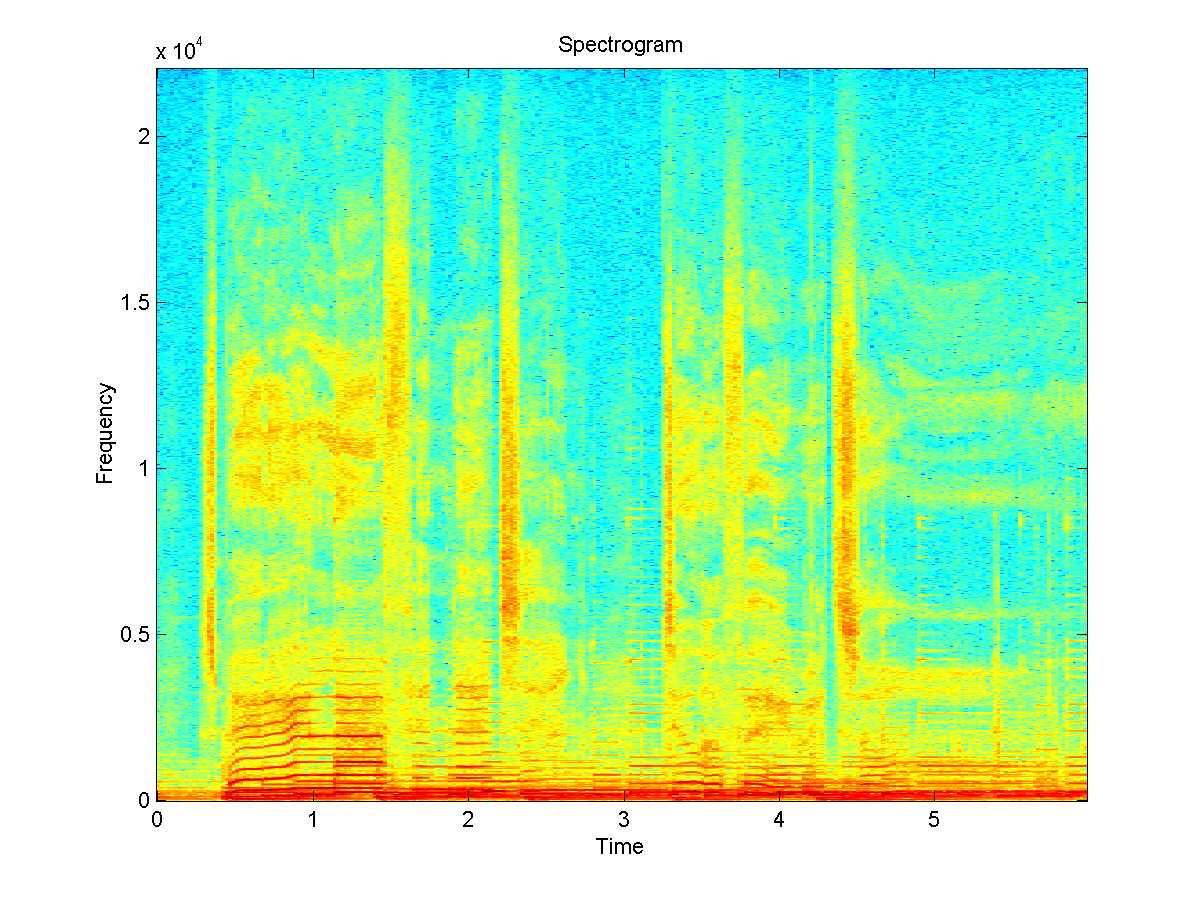
\includegraphics[scale=0.5]{Graph/specgramsignal}
			\caption[Spektrogramm eines Audiosignals]{Spektrogrammdarstellung eines Audiosignals; die roten Bereiche besitzen die h�chste Amplitude} \label{fig:specgram}
			\end{center}
		\end{figure}
    \begin{figure}[!hbt]
			\begin{center}
			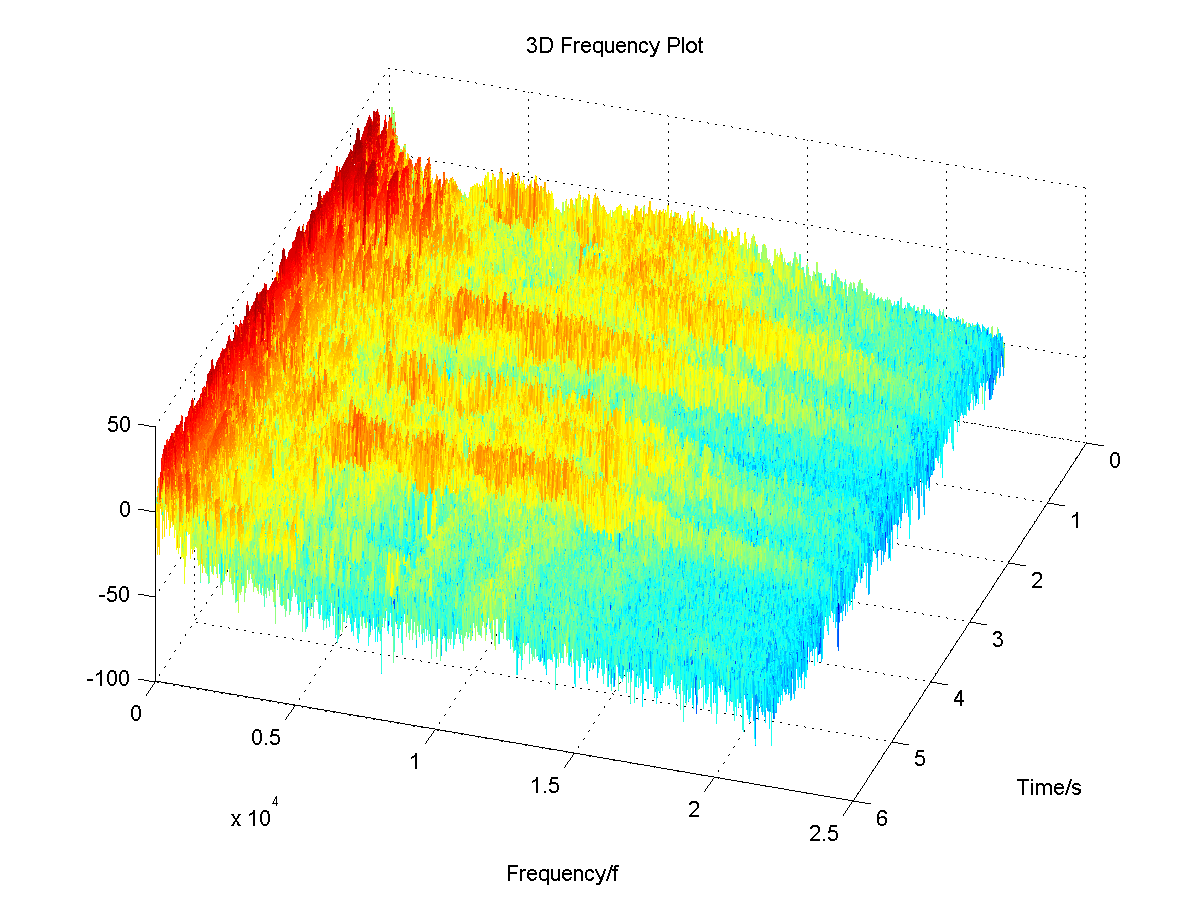
\includegraphics[scale=0.5]{Graph/3dsignal}
			\caption[3D-Frequenz/Zeitverlaufsdarstellung]{Pseudo-3D-Darstellung eines Frequenzverlaufs �ber der Zeit} \label{fig:3dsignal}
			\end{center}
		\end{figure}

\subsection{Amplitudendichteverteilung}\label{chap:adv}
	Die Amplitudendichteverteilung\index{Amplitudendichteverteilung} (ADV oder englisch: PDF f�r Probability Density Function) gibt an, wie wahrscheinlich bzw. wie h�ufig bestimmte Amplitudenwerte in einem Signal vorkommen. Dabei werden alle m�glichen Amplituden auf der Abzisse (\emp{x-Achse}) aufgetragen, und die H�ufigkeit jedes einzelnen Wertes auf der Ordinate (\emp{y-Achse}). Da ein Sprach- oder Musiksignal meistens ebenso viel positive wie negative Signalwerte besitzt, ist die ADV solcher Signale symmetrisch zur Ordinate. Best�nde ein Signal nur aus positiven Werten, so w�re auf der negativen Abszisse nur der Wert $0$ aufgetragen. Sind in einem Signal die kleineren Amplitudenwerte h�ufiger als gro�e, so wird die ADV nach au�en hin abflachen. Dies ist praktisch bei allen Sprach- und Musiksignalen der Fall. Damit die ADV sich f�r identische Signale, die aber unterschiedliche L�nge haben, nicht unterscheidet, wird sie zumeist auf die Anzahl der betrachteten Signalwerte normiert. Dies f�hrt dann dazu, da� die Summe aller normierten ADV-Werte $1$ ergibt.
	\bem{Die beschriebene Funktion ist eigentlich nur eine N�herung der ADV, n�mlich eine \emp {H�ufigkeitsverteilung}(HV)\index{H�ufigkeitsverteilung}. Lediglich die Verallgemeinerung dieser HV-Messung f�r kontinuierliche Amplitudenwerte alle Signalausdehnungen liefert dann die ADV bzw. die tats�chliche Wahrscheinlichkeitsdichtefunktion. Dennoch wird eine solche H�ufigkeitsverteilung im folgenden unter der Bezeichnung ADV verwendet.}
	\end{quote}
	\bem{Da auf der Ordinate die H�ufigkeit von Amplitudenwerten aufgetragen ist, kann kein Wert der ADV jemals negativ werden.}
	\end{quote}
    \begin{figure}[!hbt]
			\begin{center}
			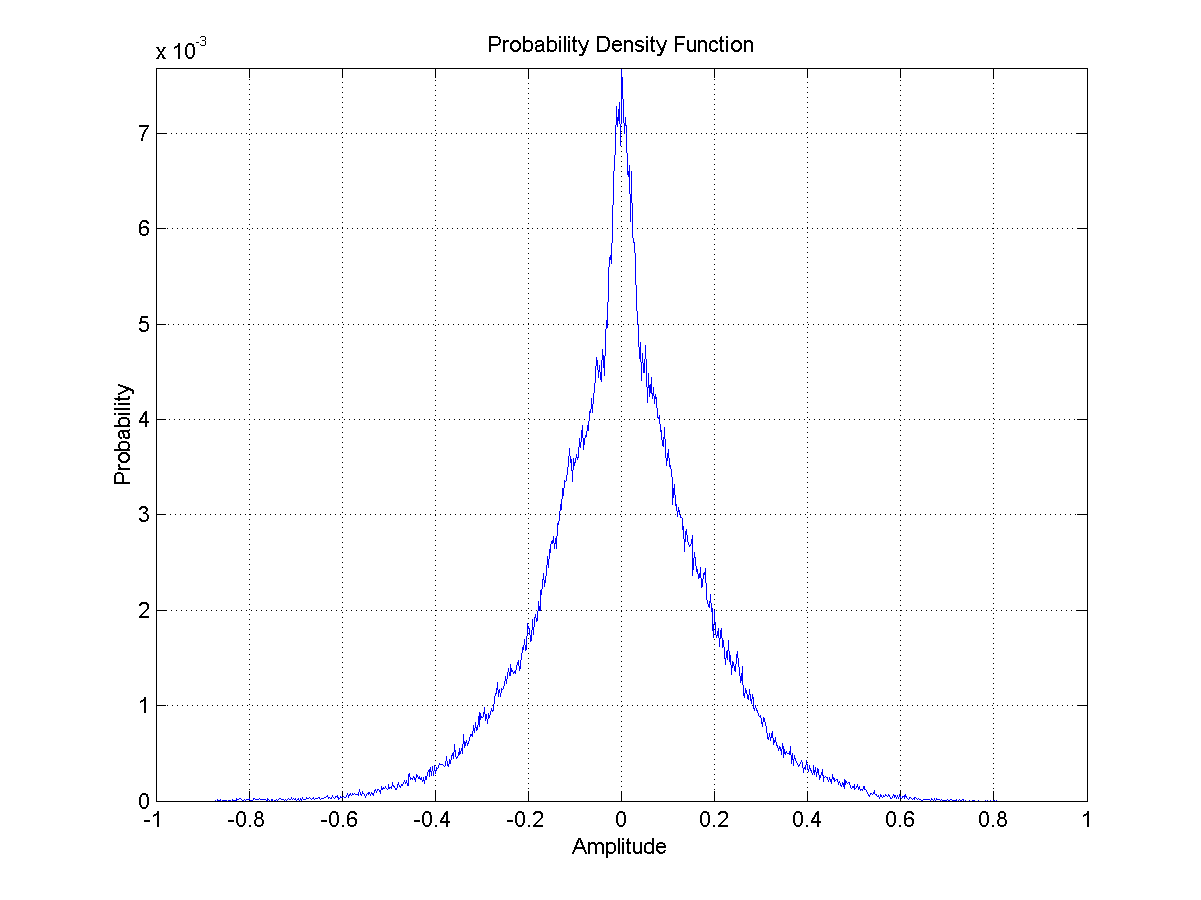
\includegraphics[scale=0.5]{Graph/pdfsignal}
			\caption[ADV eines Musiksignals]{Amplitudendichteverteilung eines Musiksignals} \label{fig:pdfplot}
			\end{center}
		\end{figure}

\section{Systembeschreibungen}
Der Begriff System\index{System} kann in der Signaltheorie f�r praktisch jedes signalverarbeitende Ger�t verwendet werden. Beispiele aus der Tontechnik sind Effekte wie Delay und Hallger�t ebenso wie ein normaler Verst�rker oder ein Kompressor (vgl. Abschnitt \ref{chap:fx}). Ebenso kann aber auch jeder Raum als System verstanden werden, der jedes akustische Signal verhallt. Der Begriff System steht also erstmal f�r eine black box mit einem vom Eingangsaudiosignal abh�ngigen Ausgang.

Der Begriff System kann also recht abstrakt f�r ziemlich viele Dinge stehen. Parameter, die ein System in seiner Grundfunktionalit�t beschreiben, sind vor allem die sog. \emp{Linearit�t}\index{Linearit�t} und die \emp{Zeitvarianz}\index{Zeitvarianz}. Ein System wird linear genannt, wenn es bestehende Signalanteile (z.B. Frequenzb�nder) des Eingangssignals verst�rkt oder d�mpft, w�hrend ein sog. nichtlineares System dem Signal zuvor nicht enthaltene Signalanteile hinzuf�gt. Beispielsweise sind Verst�rker oder Filter lineare Systeme, w�hrend ein Verzerrer oder ein Exciter nichtlineare Systeme sind.
\bem{In der Realit�t besitzt jedes analoge System wie Verst�rker und Filter auch einen nichtlinearen Anteil. Dieser Anteil soll dann m�glichst klein sein; ein Beispiel f�r die Messung der Auswirkung nichtlinearer Systemanteile (Verzerrungen\index{Verzerrung}) ist die Klirrfaktormessung (vgl. Abschnitt {chap:klirrfaktor}).}\end{quote}
Ein weiteres wichtiges Merkmal von Systemen ist ihre Zeitabh�ngigkeit. �ndern sich die Eigenschaften des Systems mit der Zeit, so nennt man das System zeitvariant, andernfalls zeitinvariant. Ein Filter ist ein zeitinvariantes System (wenn man nicht gerade die Filterparameter ver�ndert), w�hrend ein Kompressor ein zeitvariantes System ist.

\subsection{Lineare Systeme}\index{System!lineares}\label{chap:linsystem}
	Lineare Zeitinvariante System lassen sich in zwei Darstellungen beschreiben, dem \emp{�bertragungsfrequenzgang}\index{�bertragungsfrequenzgang} (auch Transferfunktion\index{Transferfunktion}) $H(f)$ und der \emp{Impulsantwort}\index{Impulsantwort} $h(t)$. Dabei gilt, da� die �bertragungsfunktion die Fouriertransformation, das Spektrum, der Impulsantwort ist. Die Impulsantwort eines Systems ist - wie der Name schon sagt - die Antwort des Systems auf einen sehr kurzen Impuls, z.B. ist die Impulsantwort eines Raumes nach einem kurzen lauten H�ndeklatschen n�herungsweise wahrzunehmen. Die Impulsantwort eines idealen Systems ist ein unendlich kurzer Impuls; der �bertragungsfrequenzgang eines idealen Systems ist ein horizontal verlaufendes Spektrum, d.h. da� jede Frequenz das System unver�ndert passieren kann.
	
\subsubsection{Faltung}\label{chap:faltung}
Mit Hilfe der Transferfunktion\index{�bertragungsfrequenzgang}\index{Transferfunktion} $H(f)$ l��t sich das Spektrum des Ausgangs $Y(f)$ aus dem Spektrum des Eingangs $X(f)$ berechnen:
\begin{equation}
	Y(f) = X(f)\cdot H(f)
\end{equation}
Da sich Spektrum und Zeitsignal beliebig ineinander �berf�hren lassen, ist der Ausgang eines linearen Systems aufgrund seiner �bertragungsfunktion\index{�bertragungsfrequenzgang}\index{Transferfunktion} leicht zu bestimmen. Am Beispiel eines Filters, der alle h�heren Frequenzen aus dem Signal herausfiltert (Tiefpa�filter), l��t sich das veranschaulichen: alle Frequenzen �ber der Grenzfrequenz $f_G$ werden abgeschnitten, w�hrend die darunterliegenden Frequenzanteile das System unbeeinflu�t passieren. Damit enth�lt das Ausgangssignal keine hohen Frequenzen mehr.\\

Wie im Frequenzbereich �ber Multiplikation l��t sich im Zeitbereich der Ausgang eines Systems $y(t)$ mit der sog. \emp{Faltung}\index{Faltung} (auch: Convolution) bestimmen. Bei der Faltungsoperation (eines Signals $x(t)$ mit einer Impulsantwort\index{Impulsantwort} $h(t)$) wird das Signal an jedem Zeitpunkt mit der Impulsantwort multipliziert und das Ergebnis �ber alle Zeitpunkte aufsummiert. Die Faltung wird in der Literatur i.a. mit einem Stern gekennzeichnet:
\begin{equation}
	y(t) = x(t)\;*\;h(t)
\end{equation}


\subsection{Nichtlineare Systeme}\index{System!nichtlineares}
Nichtlineare System k�nnen dem Signal bisher noch nicht vorhandene Anteile hinzuf�gen. Das bedeutet, nichtlineare System f�hren zu \emp{Verzerrungen}. Zu nichtlinearen Systemen gibt es keine so einfach zu verallgemeinernde Beschreibung wie f�r lineare Systeme; einen nichtlinearen Effekt kann man auf vielerlei Weise erreichen. Ein typisches Beispiel sind �bersteuerungen; aber Nichtlinearlit�ten werden auch bewu�t eingesetzt, z.B. bei Distortioneffekten, beim Kompressor oder beim Exciter.

\section{Grundlegende Signalformen bei der Signalsynthese}
Um ein besseres Gef�hl f�r Frequenzdarstellungen eines Signals zu bekommen, ist in Abb. \ref{fig:sig_spec} die Zeit- und Frequenzdarstellung von in der Klangsynthese h�ufig verwendeten tonalen Signalgrundformen dargestellt. Dabei handelt es sich um ein Sinussignal, ein Rechtecksignal, ein S�gezahnsignal und ein Dreiecksignal.
    \begin{figure}[!hbt]
			\begin{center}
			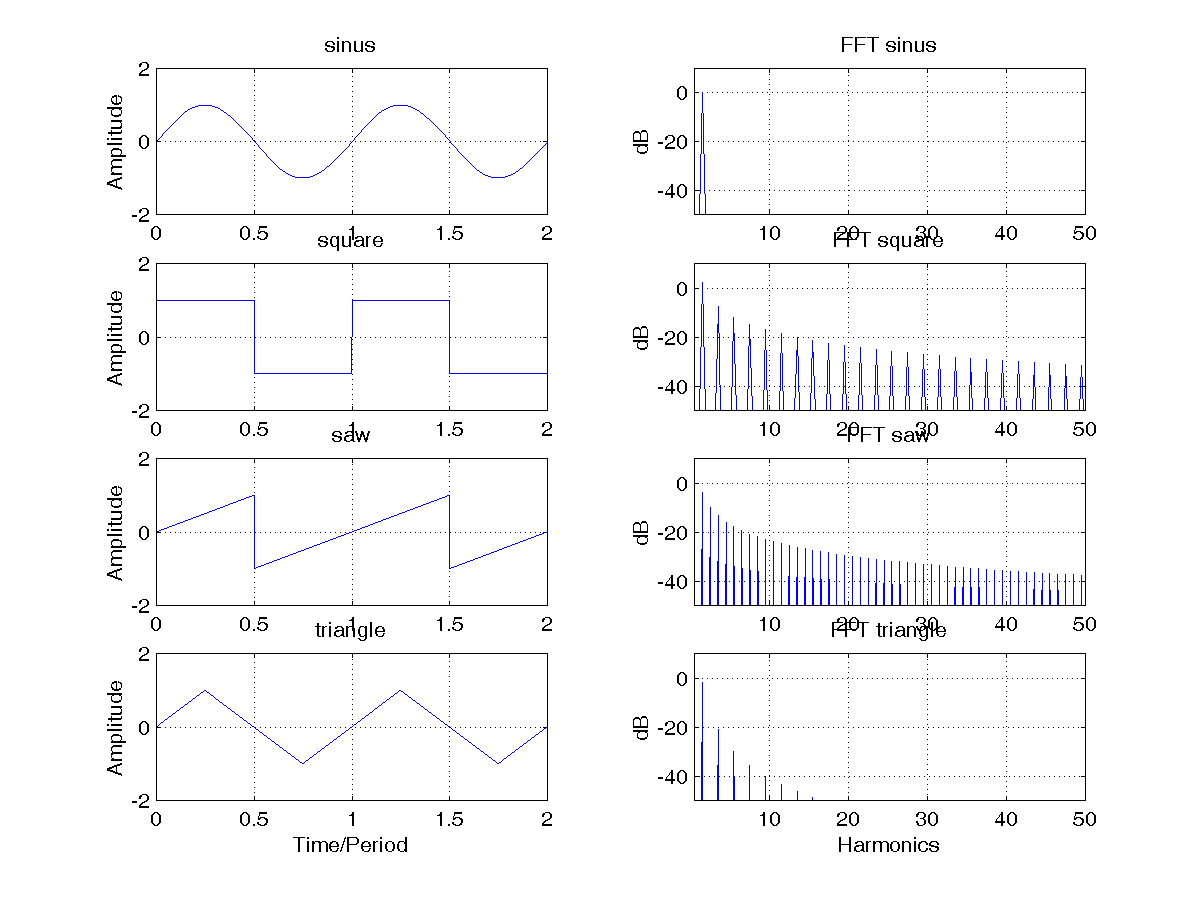
\includegraphics[scale=0.5]{Graph/signals}
			\caption[Grundsignale]{Sinus-, Rechteck-, S�gezahn-, und Dreiecksignal, links als Zeitsignal, rechts das Spektrum mit Achsenskalierung in Vielfachen der Grundfrequenz} \label{fig:sig_spec}
			\end{center}
		\end{figure}
Es ist deutlich zu sehen, da� die unterschiedlichen Signalverl�ufe in der Zeitdarstellung sich auch deutlich auf den Spektralverlauf \glqq auswirken\grqq.

\bem{Als Daumenregel kann man davon ausgehen, da� der Anteil an hohen Frequenzen immer mehr zunimmt, je pl�tzlichere oder gr��ere Spr�nge ein Signalverlauf vorweist.}\end{quote}

Eine weitere sehr wichtige, aber nicht so einfach definierbare Signalform ist das Rauschen. Die technische Definition des Rauschen besagt, da� es zu allen anderen Signalen inkoh�rent ist. Dies bedeutet z.B., da� theoretisch die Addition von zwei gleichlauten Rauschen immer nur eine Pegelerh�hung von $3dB$ ergeben kann. \\
Im Zusammenhang mit Rauschen werden oft Farben als n�here Bezeichnung f�r Rauschen verwendet, wie z.B. \emp{wei�es Rauschen} oder \emp{rosa Rauschen}. Diese Farben beschreiben den Frequenzverlauf des Rauschen und sind damit auch so eine Art Klangfarbenbeschreibung des Rauschens. 
    \begin{figure}[!hbt]
			\begin{center}
			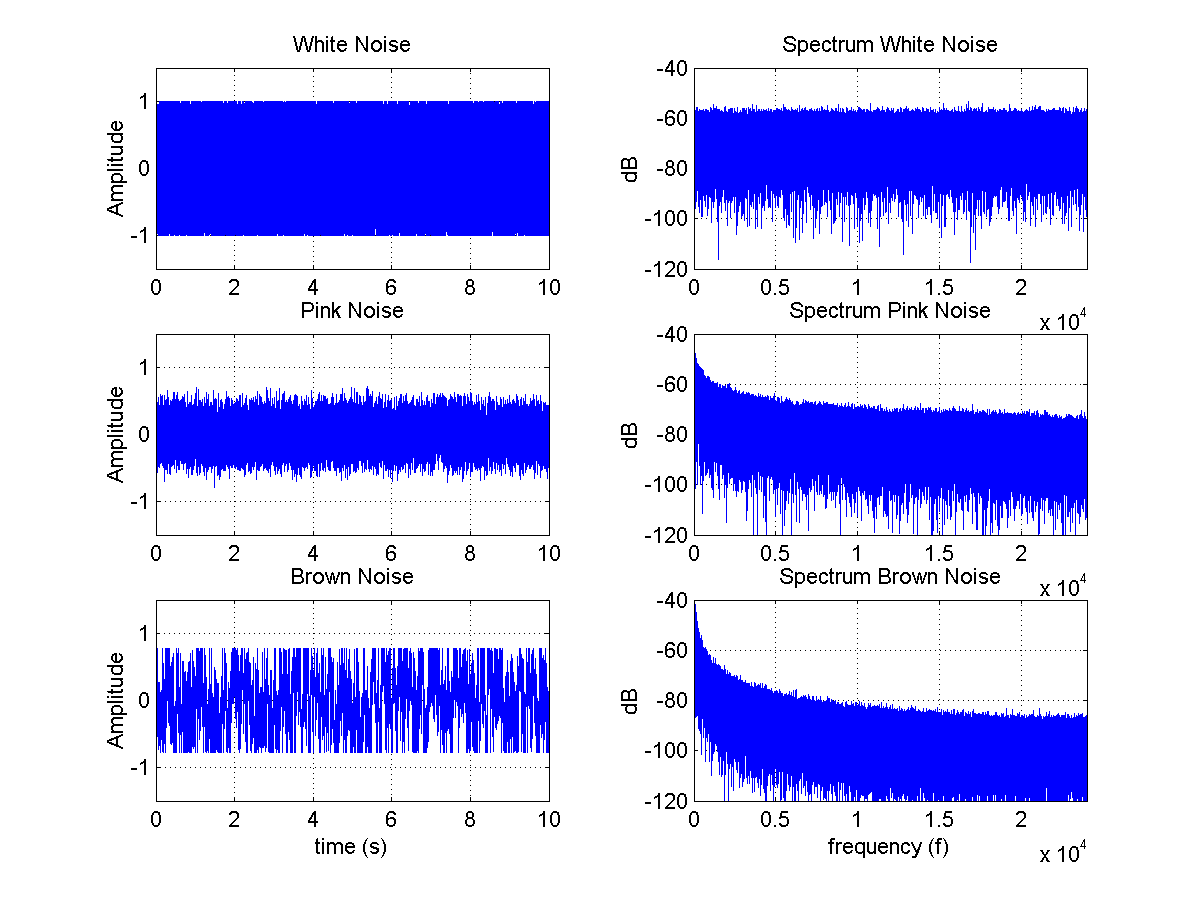
\includegraphics[scale=0.5]{Graph/noise}
			\caption[verschiedene Rauschen]{wei�es, rosa, und braunes Rauschen, links als Zeitsignal, rechts das Spektrum} \label{fig:noise_spec}
			\end{center}
		\end{figure}
Abb. \ref{fig:noise_spec} zeigt verschiedenfarbige Rauschen als Zeitsignal und in Frequenzdarstellung. Ihre Energie nimmt hin zu hohen Frequenzen folgenderma�en ab:
\begin{itemize}
	\item wei�es Rauschen\index{wei�es Rauschen}: 0dB/Octave
	\item rosa Rauschen\index{Rosa Rauschen}: 3dB/Octave
	\item braunes Rauschen\index{Braunes Rauschen}: 6dB/Octave
\end{itemize}

\section{Ger�te der Signalverarbeitung}\label{chap:fx}
In diesem Abschnitt sollen die typischen Tonstudioger�te in Ihrer Funktionsweise beschrieben werden.
	\subsection{Fader}\label{chap:fader}
	Ein \bld{Fader} ist einfach nur ein Stellregler, mit dem die Amplitude eines Signals ver�ndert werden kann. Fader findet man z.B. in Mischpulten. Sie verwenden praktisch immer eine dB-Skala, die im Bereich um 0dB besonders fein aufgel�st ist. Ein Fader ist ein lineares System und - wenn der Fader nicht bewegt wird - zeitinvariant.
\chaplink
\begin{itemize}
	\item Abschnitt \ref{chap:amplitude}
	\item Abschnitt \ref{chap:pegel}
\end{itemize}
\end{quote}

	
	\subsection{Filter}\label{chap:filter}
	\bld{Filter}\index{Filter} (auch \emp{Entzerrer}\index{Entzerrer}) sind die mit am h�ufigsten im Tonstudio eingesetzten Werkzeuge zur Klangbearbeitung und -verarbeitung.
	
	Einfache Filter zur Klangbearbeitung kennt man zum Beispiel von der Stereoanlage oder einfacher Musiksoftware, wo sich B�sse, Mitten und H�hen anheben bzw. absenken lassen. Genau das ist die Aufgabe eines Filters bzw. Entzerrers: die Anhebung oder D�mpfung bestimmter Frequenzbereiche. F�r verschiedene Einsatzbereiche m�ssen Filter verschiedene �bertragungsfunktionen haben; der Verlauf dieser �bertragungsfunktionen bestimmt den \emp{Filtertyp}. 
		
	Bevor die einzelnen Filtertypen kurz vorgestellt werden, m�ssen kurz einige Begriffe eingef�hrt werden:
	\begin{itemize}
	
	
		\item	\emp{Grenzfrequenz}\index{Grenzfrequenz}\index{Filter!Grenzfrequenz} $f_G$: Bei einseitigen Filtern die Frequenz (in $H\!z$), ab der die �bertragungsfunktion eines Filter um mehr als $\pm3dB$ von $0dB$ abweicht.
		\item	\emp{Mittenfrequenz}\index{Mittenfrequenz}\index{Filter!Mittenfrequenz} $f_C$: Bei symmetrischen Filtern die Frequenz (in $H\!z$), um die die �bertragungsfunktion des Filters symmetrisch ist.
		\item	\emp{Bandbreite eines Filters}\index{Bandbreite eines Filters} $B_G$: Bei symmetrischen Filtern die Breite des Frequenzbandes (in $H\!z$) in dem die �bertragungsfunktion um weniger als $\pm3dB$ von $0dB$ abweicht
		\item	\emp{G�te}\index{G�te}\index{Filter!G�te} $Q$: Bei symmetrischen Filtern ist die G�te ein aussagekr�ftigere Darstellung der Bandbreite. Die G�te wird berechnet durch das Verh�ltnis von 
		\begin{eq}\label{eq:guete}
			\frac{f_C}{B_G}
		\end{eq}.
		 Ist also die Bandbreite des Filters gleich der Mittenfrequenz, so nimmt die G�te den Wert $1$ an. Ist die Bandbreite schmaler als die Mittenfrequenz, so wird die G�te gr��er als $1$ und andersherum. Die G�te ist dimensionslos.
		\item	\emp{Flankensteilheit}\index{Flankensteilheit}\index{Filter!Flankensteilheit} $F$: Gibt in der Pseudo-Einheit $\left[\frac{dB}{Octave}\right]$ an, wie steil die abfallende Flanke der �bertragungsfunktion f�llt. Typische Werte sind ganzzahlige Vielfache von $6$ wie $6$, $12$, $18$ und $24\frac{dB}{Octave}$.
	\end{itemize}
	
	Filter teilt man je nach Verlauf des Betragsfrequenzganges in verschiedene Kategorien ein. Die wichtigsten sind:
	\begin{enumerate}
	
		\item	\bld{Tiefpa�-Filter}\index{Tiefpa�-Filter}\index{Filter!Tiefpa�-}:\\
		Tiefe Frequenzen bis zur Grenzfrequenz $f_G$ passieren das Filter (nahezu) unver�ndert, h�here Frequenzen werden zunehmend ged�mpft. Die St�rke der D�mpfung nimmt mit der Flankensteilheit zu. Ein typischer Wert f�r die Flankensteilheit der meisten Tiefpa�-Filter liegt bei $12\frac{dB}{Octave}$. Die einstellbaren Parameter eines Tiefpasses k�nnen sein: \emp{Grenzfrequenz}, \emp{Flankensteilheit}
				
		\item	\bld{Hochpa�-Filter}\index{Hochpa�-Filter}\index{Filter!Hochpa�-}:\\
		Alle Frequenzen �ber der Grenzfrequenz $f_G$ passieren das Filter (nahezu) unver�ndert, Frequenzen darunter werden ged�mpft. Je tiefer die Frequenz ist, desto st�rker ist die D�mpfung, die mit der Flankensteilheit zunimmt. Das Hochpa�-Filter ist das Gegenst�ck zum Tiefpa�filter, aus diesem Grund k�nnen die einstellbaren Parameter wie beim Tiefpa� \emp{Grenzfrequenz} und \emp{Flankensteilheit} sein. \\
		Sonderf�lle des Hochpa�-Filters sind der \emp{Trittschallfilter}\index{Trittschallfilter}\index{Filter!Trittschall-}, dessen Grenzfrequenz meist zwischen $50$ und $180H\!z$ liegt und der zur Unterdr�ckung von Rumpelger�uschen dient, und der \emp{DC-Block-Filter}\index{DC-Block-Filter}\index{Filter!DC-Block-} mit einer Grenzfrequenz um die $20Hz$ zur Unterdr�ckung des Gleichanteils in einem Signal.
		
		\item	\bld{Shelving-Filter}\index{Shelving-Filter}\index{Filter!Shelving-}(manchmal auch Kuhschwanz-Filter):\\
		 Das Shelving-Filter scheint sich f�r den Anwender zun�chst �hnlich zu verhalten wie Tiefpa�- oder Hochpa�filter. Ab einer bestimmten Grenzfrequenz k�nnen Frequenzen angehoben oder abgesenkt werden. Der Unterschied zu den beiden oben genannten Filtertypen ist jedoch, da� diese Anhebung/Verst�rkung oder Absenkung/D�mpfung f�r alle Frequenzen ab der Grenzfrequenz gleichstark ist und nicht mit zu-bzw. abnehmender Frequenz zunimmt. Je nachdem, ob die Anhebung oder Absenkung ober- oder unterhalb der Grenzfrequenz stattfindet, spricht man von \emp{H�henshelving} oder \emp{Tiefenshelving}. Die einstellbaren Parameter eines Shelvingfilters sind \emp{Grenzfrequenz} und \emp{Anhebung/D�mpfung} in $dB$.
		
		\item	\bld{Peak-Filter}\index{Peak-Filter}\index{Pr�senz-Filter} \index{Filter!Peak-}\index{Filter!Pr�senz-}(manchmal auch Pr�senz-Filter):\\
		 Die Aufgabe des Peakfilters ist die Anhebung oder Absenkung eines bestimmten Frequenzbandes. Dazu kann i.a. die \emp{Mittenfrequenz} des zu bearbeitenden Frequenzbandes und die \emp{G�te} (und dadurch die Bandbreite) des Filters eingestellt werden. 
		
		\item	\bld{Bandpa�-Filter}\index{Bandpa�-Filter}\index{Filter!Bandpa�-}: Das Bandpa�-Filter kann als Reihenschaltung von Tiefpa� mit hoher Grenzfrequenz und Hochpa� niedriger Grenzfrequenz interpretiert werden. Es l��t nur Frequenzen innerhalb eines bestimmten Frequenzbandes passieren. Einstellbare Parameter sind die \emp{Mittenfrequenz}, die \emp{Bandbreite} und die \emp{Flankensteilheit} des Bandpasses.
		
		\item	\bld{Bandsperre-Filter}\index{Bandsperre-Filter}\index{Filter!Bandsperre}:\\
		 Die Bandsperre ist das genaue Gegenteil des Bandpasses; alle Frequenzen, die nicht innerhalb eines bestimmten Frequenzbandes liegen, k�nnen das Filter (nahezu) ungehindert passieren. Frequenzen innerhalb des Frequenzbandes werden unterdr�ckt. Die einstellbaren Parameter sind wie beim Bandpa� die \emp{Mittenfrequenz}, die \emp{Bandbreite} und die \emp{Flankensteilheit}.
		
		\item	\bld{Notch-Filter}\index{Notch-Filter}\index{Filter!Notch-}:\\
		 Das Notchfilter kann aus Anwendersicht als Spezialfall der Bandsperre mit einem sehr schmalen Frequenzband interpretiert werden. Alle Frequenzen bis auf eine ganz spezielle k�nnen das Filter (nahezu) ungehindert passieren, diese Frequenz wird komplett herausgefiltert. Als Parameter l��t sich zumeist nur die \emp{Mittenfrequenz} einstellen, manchmal auch die \emp{G�te} des Filters.\\
		 Der Einsatzzweck eines Notch-Filters ist zum Beispiel das Herausfiltern von st�rendem Netzbrummen von einer Aufnahme. Dabei werden meistens mehrere Notchfilter eingesetzt, deren Mittenfrequenzen ganzzahlige Vielfache der Grundfrequenz sind, da Netzbrummen normalerweise nicht nur aus einem sinusf�rmigen Signal besteht.\\
		 Die Phasenverschiebungen um die Mittenfrequenz sind bei einem Notch-Filter sehr stark, und das gefilterte Signal sollte nach der Bearbeitung daraufhin �berpr�ft werden.
		 
	\end{enumerate}
	Verschiedene dieser Filter (v.a. Tiefpa� und Bandpa�) gibt es auch als sogenannte \emp{Resonanz-Filter}\index{Resonanz-Filter}\index{Filter!Resonanz}. Diese zeichnen sich dadurch aus, da� sie an der Grenzfrequenz bzw. der Mittenfrequenz noch eine starke (regelbare) Anhebung haben. Dadurch wird klanglich diese Frequenz betont, was insbesondere bei Filterungen interessant ist, wo zeitliche Ver�nderungen der Grenzfrequenz/Mittenfrequenz als musikalisches Stilmittel eingesetzt werden.
	
	Filter unterschiedlicher Hersteller klingen im allgemeinen unterschiedlich. Diese Klangunterschiede sind das Resultat unterschiedlicher Herangehensweise beim Filterentwurf. Bei analogen Filtern spielen auch die verwendeten Bauteile eine Rolle. Diskussionsstoff liefert oft auch der Phasenfrequenzgang eines Filters. Hier l��t sich nicht abschlie�end sagen, welchen Einflu� dieser auf die empfundene Qualit�t eines Filters hat. Filter mit linearen Phasengang sind in der Analogwelt nicht realisierbar. Ein Filter ist ein lineares System und - wenn die Parameter nicht ge�ndert werden - zeitinvariant.
	
	Mit dem Einsatz von Filtern lassen sich auch andere Effekte erreichen, wie z.B. der \bld{Phaser}\index{Phaser}-Effekt. Dieser Effekt l�sst sich erreichen durch eine Reihenschaltung mehrerer Notch-Filter mit unterschiedlichen Mittenfrequenzen. Dieser Mittenfrequenzen werden durch einen Oszillator leicht moduliert. Die starken Phasenverschiebungen um die Mittenfrequenz des Notchfilters f�hren bei der Addition mit dem Originalsignal zu Interferenzen (vgl. Abschnitt \ref{chap:phaseshift}, die sich zeitlich mit der Frequenz des Oszillators ver�ndern.

\chaplink
\begin{itemize}
	\item Abschnitt \ref{chap:local}
	\item Abschnitt \ref{chap:ton_klang}
	\item Abschnitt \ref{chap:phaseshift}
\end{itemize}
\end{quote}
	
	\subsection{Delay und Delay-basierte Effekte}\index{Delay}\label{chap:delay}
		Das \bld{Delay} ist ein Effekt, der schon seit langer Zeit insbesondere im Pop-/Rock\-bereich eingesetzt wird. Im einfachsten Fall wird dieser Effekt erzeugt, indem das Eingangssignal verz�gert wird und ged�mpft dem Originalsignal hinzugemischt wird. Je nach Intensit�t des verz�gerten Signals und der Verz�gerungszeit entsteht so oft der Eindruck eines Echos\index{Echo} (vgl. Abschnitt \ref{chap:firstfront} zur Echoschwelle). Auch wenn man diesen einfachen Fall schon als Delayeffekt bezeichnen kann, so sind die i.a. eingesetzten Delayeffekte noch etwas ausgefeilter. Der typische Delayeffekt ist r�ckgekoppelt, d.h. der Ausgang des Effekts wird (etwas ged�mpft) wiederum auf ein Verz�gerungsglied gegeben. Auf diese Art und Weise erreicht man ein st�ndig leiser werdendes Ausklingen. Abh�ngig von den Einstellungen (Zeit der Verz�gerung, D�mpfung des verz�gerten Signals) l��t sich die L�nge und die Dichte des Effekts von einem beatweise wiederholen bis zum hall�hnlichen Nachklang variieren. \\
Ein Delay ist i.a. ein lineares System und meistens zeitinvariant.

Andere Effekte bauen auf der zeitlichen Ver�nderung der Verz�gerungszeit auf. Der \bld{Flanger\index{Flanger}} arbeitet zumeist mit einer Zeit $<15ms$, die kontinuierlich - beispielsweise sinusf�rmig - moduliert werden. Die Modulationsgeschwindigkeit liegt in der Gr��enordnung von $1H\!z$.\\
Der \bld{Chorus}\index{Chorus} �hnelt dem Funktionsprinzip des Flangers sehr. Hier wird aber nicht nur ein verz�gertes Signal auf das Originalsignal addiert, sondern mehrere mit unterschiedlichen Delayzeiten (meistens zwischen $10$ und $25ms$). Die Verz�gerungszeiten werden dabei st�ndig leicht ver�ndert. Im Gegensatz zum Flanger sind diese kleinen �nderungen zuf�llig, und werden nicht vom einem deterministischen Signal wie einem Sinus hervorgerufen.\\
Flanger und Chorus sind lineare zeitinvariante Systeme. Klanglich ist der Phaser\index{Phaser} ein verwandter Effekt.

\chaplink
\begin{itemize}
	\item Abschnitt \ref{chap:firstfront}
\end{itemize}
\end{quote}
		
	\subsection{Hallger�t}\label{chap:reverb}\index{Hall}\index{Hallger�t}
		Aufgabe eines \bld{Hallger�tes} ist es, das Eingangssignal in einer Weise zu verarbeiten, da� es mit einem r�umlichen Eindruck versehen wird, wie eine Schallquelle in einem Raum. Technisch gesprochen versucht ein Hallger�t die Raumimpulsantwort eines Raumes nachzubilden, und das Eingangssignal mit dieser zu falten. Es existieren auch Hallger�te, die auf real gemessenen Rauminpulsantworten beruhen, und die das Eingangssignal mit dieser Impulsantwort falten. Zur Optimierung des Halls f�r das spezielle Eingangssignal und die Anwendung werden meistens die unterschiedlichsten R�ume als Presets angeboten, die dann mit verschiedenen Parametern angepa�t werden k�nnen. Die wichtigsten Parameter sind hierbei die Nachhallzeit\index{Nachhallzeit}, verschiedene Filterparameter insbesondere zur Tiefenanhebung/-absenkung oder Hochpa�filterung und das sogenannte Pre-Delay\index{Pre-Delay}, mit dem sich eine Verz�gerung des verhallten Signals erzielen l��t.\\
Ein Hallger�t ist ein lineares System und - wenn die Parameter nicht ge�ndert werden - zeitinvariant.

\chaplink
\begin{itemize}
	\item Abschnitt \ref{chap:raumak}
	\item Abschnitt \ref{chap:faltung}
\end{itemize}
\end{quote}

	\subsection{Dynamikbearbeitung}\label{chap:dynamics}
		Ger�te zur Dynamikbearbeitung\index{Dynamikbearbeitung} regeln im allgemeinen die Verst�rkung/D�mpfung f�r ein bestimmtes Eingangssignal automatisch in Abh�ngigkeit des Eingangspegels. Dazu kann man bei fast allen Ger�ten die sogenannte \emp{Attack Time}\index{Attack Time} und \emp{Release Time}\index{Release Time} einstellen. Die Attack Time ist eine Zeitkonstante zur Einstellung der Reaktionszeit des Systems auf pl�tzliche Peaks oder laute Passagen, w�hrend �ber die Release Time die Reaktionszeit beim Wechsel von lauten hin zu leisen Passagen einstellbaren ist. Bekannte Ger�te zur Dynamikbearbeitung sind:
		\begin{enumerate}
			\item	\bld{Noise Gate}\index{Noise Gate}:\\
				Die Aufgabe eines Noise Gates ist, bei Signalen mit einem geringeren Pegel als der eingestellten \emp{Threshold} kein Signal auszugeben, bei lauteren Signalen das Signal allerdings unver�ndert zu lassen. Dies geschieht �ber einen pegelabh�ngigen \emp{Gain Factor} der sich allerdings nicht unmittelbar �ndert. Oft lassen sich auch �ber die \emp{Attack Time} und die \emp{Release Time} die Reaktionszeiten des Systems einstellen. Zu kurze Zeiten f�hren hierbei oft zu einem zerst�ckelten Klang, w�hrend zu lange Reaktionszeiten entweder dazu f�hren, da� der Anfang relevanter, laute, Passagen fehlt oder das Gate bei nichtgewollten Signalen mit kleinem Pegel zur sp�t \glqq zumacht\grqq.
			\item \bld{Limiter}\index{Limiter}:\\
				Ein Limiter soll starke Peaks eines Signals kontrollieren (insbesondere um �bersteuerungen zu vermeiden), das Eingangssignal und seinen Dynamikbereich aber m�glichst unver�ndert lassen. Hierzu mu� die Reaktionszeit des Systems insbesondere f�r die Detektion von lauten Signalanteilen m�glichst kurz sein. Wird der Eingangspegel des Signals bei gleichen Limitereinstellungen angehoben, so resultiert dies sowohl in einer Lautst�rkeerh�hung des Signals als auch in einigen zus�tzlichen hohen Frequenzenanteilen.
			\item	\bld{Compressor}\index{Compressor} und \bld{Expander}\index{Expander}:\\
			  Compressoren sind mit die am h�ufigsten eingesetzten Ger�te zur Dynamikbearbeitung. Sie werden zur Eingrenzung des Dynamikumfangs benutzt. Signalanteile mit kleinem Pegel passieren das System unbeeinflu�t, w�hrend hohe Pegel oder laute Teile entsprechend der Kompressorkennlinie ged�mpft werden. Durch Anhebung des Eingangspegels kann so ein lauteres Signal mit geringem Dynamikumfang erreicht werden.\\
			  Expander tun genau das Gegenteil von Kompressoren; sie senken leise Signalanteile im Pegel ab, w�hrend sie laute Signalanteile anheben. Das Resultat ist eine \glqq lebendigere\grqq$\;$ Klangcharakteristik.
				
		\end{enumerate}
		Es gibt eine ganze Reihe Effektger�te oder PlugIns, die prinzipiell zur Familie der Dynamikprozessoren geh�ren, aber aufgrund von Modifikationen im Algorithmus und anderen Gr�nden anders genannt werden. M�gliche Namen sind z.B. Finalizer, Maximizer, etc. 

Die Ger�te zur Dynamikbearbeitung sind i.a. nichtlineare und zeitvariante Systeme.
\chaplink
\begin{itemize}
	\item Abschnitt \ref{chap:ss-pegel}
	\item Abschnitt \ref{chap:lautstaerke}
\end{itemize}
\end{quote}

	\subsection{Verzerrer und Enhancer}
	\subsection{andere Effekte}
		Ein sog. \bld{De-Esser}\index{De-Esser} wird zur Verarbeitung von Sprache und Gesang verwendet. Bei diesen Signalen werden die Zisch- und S-laute oft als zu dominant und st�rend empfunden. Die Aufgabe eines De-Essers ist es, diese Signalanteile, die meistens im Bereich zwischen $2$ und $6kH\!z$ liegen, zu d�mpfen. Hierzu wird meistens ein Filter verwendet, dessen D�mpfung abh�ngig von der Signalamplitude in diesem Frequenzbereich ist.\\
		
R�hrensimulation, Tape Saturation	

\section{Qualit�tsmerkmale}
	Die Einsch�tzung der Qualit�t von verwendetem Equipment kann sehr wichtig sein. Wenn man selbst keine Messungen durchf�hren kann oder will, ist man zumeist auf Tests in Fachzeitschriften und die Herstellerangaben angewiesen. Die dabei h�ufig angegebenen Daten sollen in diesem Abschnitt kurz erl�utert werden. 

\subsection{�bertragungsfrequenzgang}\label{chap:transferfunc}	
	Der \bld{�bertragungsfrequenzgang}\index{�bertragungsfrequenzgang} eines Ger�tes ist v.a. bei Verst�rkern oder (elektroakustischen) Wandlern von Interesse, da diese - im Gegensatz zu Effekten - das Signal m�glichst wenig beeinflussen sollen. Angestrebt wird daher ein m�glichst linearer Frequenzgang �ber einen m�glichst gro�en Frequenzbereich. Die Linearit�t wird dabei meist durch die maximale Abweichung (wie z.B. $\pm0.5dB$) vom idealen (horizontal) verlaufenden Frequenzgang angegeben. Dazu wird der Frequenzbereich (z.B. $15H\!z$ - $22kH\!z$ angegeben, f�r den diese maximale Abweichung gilt. Diese Angaben lassen allerdings keine R�ckschl�sse auf den Phasengang des Systems zu.
	
	Die (Hersteller-)Angabe eines Frequenzganges ist umso aussagekr�ftiger, je h�her die Aufl�sung der dB-Skala ist. Manchmal wird der Frequenzgang auf einer Skala mit derma�en hoher Aufl�sung gezeigt, da� eine Aussage �ber seine Linearit�t gar nicht mehr m�glich ist. Auch durch Verdickung der aufgetragenen Linie wirkt der Frequenzgang f�r das Auge des fl�chtigen Betrachters zun�chst linear, obwohl er das nicht sein mu�.

\subsection{Dynamikumfang}
	Der \bld{Dynamikumfang}\index{Dynamikumfang} eines Systems ist leicht vereinfacht gesagt der Pegelwert, um den ein vollausgesteuertes Signal ged�mpft werden kann, bis es im Grundrauschen des Systems verschwindet. Dieser Wert ber�cksichtigt keine nichtlinearen Verzerrungen und wird in dB angegeben. Dieser Wert ist vergleichbar zum Signal-Rauschabstand (SNR)\index{Signal-Rauschabstand} eines Systems.
	
\subsubsection{Bewertungsfilter}
	Das Ohr hat, wie in Abschnitt \ref{chap:lautstaerke} beschrieben, keinen linearen Frequenzgang. Die spektrale Verteilung des Systemrauschens bei der Messung des Dynamikumfangs wird bei einer Messung wie oben beschrieben allerdings nicht ber�cksichtigt. Wenn das Rauschen beispielsweise sehr starke Anteile oberhalb von $12kH\!z$ h�tte, so w�rden diese genauso stark gewichtet wie Anteile um $3kH\!z$, was nicht dem subjektiven menschlichen Lautst�rkeempfinden entspr�che.\\
	Aus diesem Grund gibt es die sogenannten \bld{Bewertungsfilter}\index{Bewertungsfilter}\index{Filter!Bewertungs-} oder \bld{Gewichtungsfilter}\index{Gewichtungsfilter}\index{Filter!Gewichtungs-}, welche grob den Verlauf der Kurven gleicher Lautst�rkepegel approximieren. Die in der Tonme�technik am h�ufigsten verwendete Bewertungskurve ist die sogenannte \emp{A-Bewertung}, da diese der Empfindlichkeit des Ohres f�r geringe Pegel nachempfunden ist. Die B- und C-Kurven sind f�r Messungen bei mittlerem bzw. hohem Pegel gedacht. Werte, die mit A-Bewertung gemessen wurden, werden durch ein angeh�ngtes A kenntlich gemacht, z.B. $95dB(A)$\index{Dezibel!dB(A)} oder $110dB(C)$\index{Dezibel!dB(C)}. Zu beachten ist, da� A-bewertete Messungen praktisch immer \glqq bessere\grqq$\,$ Ergebnisse liefern als unbewertete.\\
	Als alternative Bewertungskurve zu der A-Bewertung existiert noch die CCIR-Bewertungskurve. 
\chaplink
\begin{itemize}
	\item Abschnitt \ref{chap:ss-pegel}
\end{itemize}
\end{quote}

\subsection{Klirrfaktor}\label{chap:klirrfaktor}
	Der \bld{Klirrfaktor}\index{Klirrfaktor} (englisch: \emp{THD} f�r \emp{Total Harmonic Distortion}) eines Systems ist ein Ma� f�r seine nichtlinearen Verzerrungen. Ein nichtlineares System erzeugt Verzerrungen bei Frequenzen, die ganzzahligen Vielfachen der Eingangsfrequenz entsprechen. Zur Messung des Klirrfaktors wird an den Eingang des Systems ein Sinussignal (meistens der Frequenz $1000H\!z$ gelegt. Der Klirrfaktor $k$ berechnet sich dann mit
	\begin{equation}
		k = \sqrt{k_2^2 + k_3^2},
	\end{equation}
	wobei die Summanden das Verh�ltnis des Spannungswertes bei der n-fachen Grundfrequenz und der Gesamtspannung des Systems $U_{ges}$ sind:
	\begin{equation}
		k_n = \frac{U_n}{U_{Ges}}
	\end{equation}
	Der Pegel des Sinustons ist von immenser Bedeutung f�r die Aussagekraft der Messung. Im allgemeinen w�chst der Klirrfaktor mit zunehmendem Eingangspegel, so da� die Messung m�glichst bei Vollaussteuerung durchgef�hrt werden sollte.
	
	Manchmal wird statt des Klirrfaktors auch das sogenannte \emp{Klirrd�mpfungsma�}\index{Klirrd�mpfungsma�} $a_k$ angegeben:
	\begin{equation}
		a_k = 20\log\left(\frac{1}{k}\right)
	\end{equation}
	
	
\subsection{Total Harmonic Distortion and Noise}
	Die Messung des \bld{THD+N}\index{Total Harmonic Distortion and Noise}-Wertes ist wie der Klirrfaktor ein Ma� f�r die nichtlinearen Verzerrungen, ber�cksichtigt aber auch das Rauschen des Testsystems. Im Falle eines idealen linearen Systems (ohne nichtlineare Verzerrungen) entsprechen die THD+N-Werte dem Dynamikumfang des Systems.
	
\subsection{Modulationsverzerrungen}
		Durch eine nichtlineare Verzerrung entstehen nicht nur harmonische Vielfache der Grundfrequenz, sondern auch sogenannte Summen- und Differenzt�ne, die bei der Klirrfaktormessung nicht ber�cksichtigt werden. Die St�rke dieser Verzerrungen versucht man mit dem kaum mehr gebr�uchlichen \bld{Intermodulationsfaktor}\index{Intermodulationsfaktor}, f�r dessen Messung die Summe der Spannungen an den Frequenzen der Summen- und Differenzt�ne gebildet wird, oder mit dem sog. \bld{Differenztonfaktor}\index{Differenztonfaktor} zu messen. Der Differenztonfaktor gibt das Verh�ltnis von der Spannung bei den Differenztonfrequenzen zu der Gesamtspannung an. Es k�nnen verschiedene Ordnungen des Differenztonfaktors angegeben werden:
		\begin{eqnarray}
			d_2 &=& \frac{U_{f_2-f_1}}{\sqrt{2}\cdot U_{Ges}} \\
			d_3 &=& \frac{U_{2f_2-f_1} + U_{2f_1-f_2}}{\sqrt{2}\cdot U_{Ges}} 
		\end{eqnarray}
Die Differenz von $f_2$ und $f_1$ sollte dabei $70H\!z$ betragen.

\subsection{�bersprechd�mpfung}	
	Die \bld{�bersprechd�mpfung}\index{�bersprechd�mpfung} eines mehrkanaligen Systems gibt an, mit welcher D�mpfung in dB das Audiosignal eines Kanals auf dem anderen zu h�ren ist. �bersprechen sollte in digitalen Ger�ten nicht auftreten.

\subsection{H�rtests}\label{chap:listtest}
	Mit den beschriebenen Merkmalen lassen sich zeitvariante Systeme kaum in Ihrer Qualit�t beurteilen. Desweiteren sind auch Systeme vorstellbar, die technisch schlechtere Me�werte aufweisen, aber dennoch subjektiv besser klingen. Um solche Qualit�tskriterien besser in den Griff zu bekommen, kann man H�rtests durchf�hren, bei denen die Testh�rer die Qualit�t (u.U im Vergleich zu einem Referenzsignal) aufgrund ihres subjektiven Eindrucks beurteilen. Insbesondere f�r Systeme wie AD/DA-Wandler (vgl. Abschnitt \ref{chap:wandler}) oder Codierungsverfahren (vgl. Abschnitt \ref{chap:codecs}) sind solche H�rtests von Bedeutung. 
	
	Die Durchf�hrung von H�rtests ist aber zumeist sehr aufwendig, wenn die Ergebnisse aussagekr�ftig sein sollen. In der Vorbereitung mu� man sich genaue Gedanken machen �ber die Auswahl des Testmaterials, die Auswahl und Menge der Testh�rer, die Testmethode (Bewertungsskala, Referenzsignal, etc.), die Testbedingungen wie z.B. die verwendeten Kopfh�rer oder Lautsprecher und die Akustik des Raums und letztendlich auch die Methode zur statistischen Auswertung dieser Tests. Aufgrund dieser Komplexit�t bei Planung und Durchf�hrung eines H�rtests sowie um Ergebnisse unterschiedlicher H�rtests miteinander vergleichbar zu machen, gibt es internationale Standards, die sich mit genau dieser Thematik auseinandersetzen (s. z.B. \cite{bs.1116}).

\chaplink
\begin{itemize}
	\item Abschnitt \ref{chap:wandler}
	\item Abschnitt \ref{chap:codecs}
\end{itemize}
\end{quote}

\section{Zusammenfassung}
	Es existieren verschiedene M�glichkeiten, ein Audiosignal und seine Eigenschaften darzustellen. Die wichtigsten sind der \bld{Zeitverlauf}, bei dem die Amplitudenwerte �ber der Zeit aufgetragen werden, verschiedene Formen des \bld{Spektrums}, wo meistens die Amplitude einer bestimmten Frequenz f�r alle im Signal enthaltenen Frequenzen angezeigt wird, und die Darstellung in Form der \bld{Amplitudendichteverteilung}, wo die H�ufigkeit bestimmter Amplitudenwerte �ber das Signal bestimmt wurden.\\
	Jedes Ger�t in der Tontechnik, sei es ein Effektger�t, ein Mischpult, ein Mikrophon oder ein Lautsprecher, selbst ein Raum kann technisch als \bld{System} interpretiert werden. F�r Systeme sind die �bergeordnetsten Kategorien \bld{Linearit�t}/bld{Nichtlinearit�t} und \bld{Zeit(in-)varianz}. Nichtlineare Systeme f�gen im Gegensatz von linearen Systemen neue Frequenzanteile in ein Signal ein. Der Ausgang von linearen und zeitinvarianten Systemen l��t sich �ber die sogenannte \bld{Faltung} berechnen.\\
Es existieren Studioger�te f�r die unterschiedlichsten Einsatzbereiche. Diese k�nnen sowohl linear als auch nichtlinear, sowohl zeitinvariant als auch zeitvariant sein.\\
Bei der Messung von Audioqualit�t ist es von gro�er Wichtigkeit, die von Hersteller angegebenen Werte richtig zu interpretieren. Die wichtigsten Punkte sind hier der lineare \bld{�bertragungsfrequenzgang}, der \bld{Dynamikumfang} und geringe \bld{nichtlineare Verzerrungen}.

\section{Aufgaben}
\begin{enumerate}
	\item Warum ist ein Fader ein lineares System, obwohl seine Skala doch nichtlinear ist?
	
	\item	Berechne die G�te $Q$ eines Filters mit der Mittenfrequenz $3.2kH\!z$ mit folgenden Bandbreiten:
		\begin{itemize}
			\item	$1600H\!z$,
			\item	$3200H\!z$,
			\item	$4000H\!z$
			\item	$6400H\!z$
		\end{itemize}
	
	\item	Ab welcher Frequenz ist bei einem Tiefpa� mit der Grenzfrequenz $100H\!z$ und der Flankensteilheit $12\frac{dB}{Octave}$ die D�mpfung gr��er als $15dB$?
	
	\item	Auf welche Zeitspanne mu� die Verz�gerungszeit eines Delayeffekts gestellt werden, wenn der Effekt \glqq im Takt\grqq$\;$ klingen soll und das Musikst�ck ein Tempo von 90 Schl�gen pro Minute (BPM = Beats per minute) besitzt?
	
	\item Auf wieviel Prozent mu� der Anteil des R�ckkopplungszweiges eines Delayeffekts gesetzt werden, wenn der Pegel jeder R�ckkopplung um $6dB$ abnehmen soll?
	
	\item Mit dem Pre-Delay verz�gert man das verhallte Signal gegen�ber dem trockenen, unverhallten Signal. Wird bei Erh�hung des Pre-Delays der Gesamteindruck eher nach hinten, in die Tiefe des Raums rutschen oder im Gegenteil pr�senter bzw. n�her klingen?
	
	\item Compressor-Einstellung
	
\end{enumerate}

\nocite{zoelzer, eargle}
%
	\chapter{Elektroakustische Wandler}
\thispagestyle{empty}
Der Sinn eines elektroakustischen Wandlers ist die Umwandlung einer physikalischen Gr��e
    des Schallfeldes wie z.B. den Schalldruck oder die Schallschnelle in eine elektrische Gr��e wie z.B. eine Spannung umzuwandeln, oder umgekehrt (Schallsender). Alle in der Tonstudiotechnik
    gebr�uchlichen Wandler besitzen eine Membran, welche durch das Schallfeld in Schwingungen
    versetzt wird, und einen elektrischen Teil, der diese mechanischen Schwingungen in
    elektrische Schwingungen wandelt. 
    
\section{Mikrophone}
Mikrophone als Schallempf�nger wandeln also akustische Energie in elektrische Energie.\\
Einflu� auf den Proze� dieser Wandlung haben sowohl der \emp{mechanische Aufbau} als auch der \emp{elektrische Aufbau} des Mikrophons. Diesen beiden Teile werden, nach einer kurzen Erl�uterung einiger grundlegender Wandlerkenngr��en, umfassend behandelt. Anschlie�end wird der Einflu� der Bauform auf das Mikrophons erl�utert.

\subsection{Charakteristische Kenngr��en}
	\subsubsection{Pegel-Kenngr��en}
	Die in Mikrophondatenbl�ttern angegebenen Gr��en sind oft einzahlige Pegelwerte, deren Aussage im folgenden kurz beschrieben werden soll.
\begin{itemize}
		\item \bld{Feld�bertragungsfaktor}\index{Feld�bertragungsfaktor|bld}\\
		Der Feld�bertragungsfaktor gibt den Effektivwert der Ausgangsspannung an, wenn das Mikrophon einem Schalldruck von $1Pa$ bei einer Frequenz von $1kH\!z$ ausgesetzt wird (in [V] oder [dBV]).

		\item	\bld{Grenzschalldruckpegel}\index{Grenzschalldruckpegel|bld}\\
		Der Grenzschalldruckpegel eines Mikrophons ist der Schalldruckpegel, ab dem der Klirrfaktor gr��er als $0.5\%$ wird (in [dBSPL]).
\chaplink
\begin{itemize}
	\item Abschnitt \ref{chap:klirrfaktor}
\end{itemize}
\end{quote}

		\item	\bld{Maximaler Ausgangspegel}\index{Ausgangspegel!maximaler|bld}\\
		Der maximale Ausgangspegel gibt den Effektivwert der Spannung am Ausgang des Mikrophons beim Grenzschalldruck an (in [V] oder [dBu]).

		\item \bld{Eigenst�rspannung}\index{Eigenst�rspannung|bld}\\
		Die Eigenst�rspannung ist die effektive Ausgangsspannung des Mikrophons, wenn es keinem Schall ausgesetzt ist (in [V] oder [dBu]).
		
		\item	\bld{Ersatzger�uschpegel}\index{Ersatzger�uschpegel}\\
		\item	\bld{Ger�uschpegelabstand}\index{Ger�uschpegelabstand}\\
		\item	\bld{Dynamikumfang}\index{Dynamikumfang}\\
		Der Dynamikumfang ergibt sich aus der Differenz zwischen Grenzschalldruckpegel und Ersatzger�uschpegel.

\end{itemize}

	\subsubsection{�bertragungsfrequenzgang}
		Ein wichtiges Merkmal zur Charakterisierung eines Mikrophons ist nat�rlich sein �bertragungsfrequenzgang\index{�bertragungsfrequenzgang} (vgl. \ref{chap:transferfunc}). Soll das Mikrophon das Schallereignis neutral �bertragen, so ist nat�rlich ein linearer Frequenzgang  mit gleichbleibendem Feld�bertragungsma� f�r alle Frequenzen w�nschenswert. Es werden allerdings in vielen F�llen bewu�t auch Mikrophone mit Abweichungen von diesem Frequenzgang produziert und eingesetzt, da sich auf diese Weise ein anderer, gew�nschter Klangeindruck erzielen l��t.
		
		Bei der Angabe des �bertragungsfrequenzganges eines Mikrophons wird zumeist nicht nur eine einzelne Kurve angegeben, sondern mehrere f�r den Schalleinfall aus verschiedenen Richtungen. Diese sind sogenannte \bld{Freifeldfrequenzg�nge}\index{Freifeldfrequenzgang}.
	
	Freifeld/Diffusfeld
	
	Der �bertragungsfrequenzgang eines Mikrophons setzt sich haupts�chlich aus zwei Komponenten zusammen: die �bertragungsfunktion des \emp{mechanischen Aufbaus} und die des \emp{elektrischen Aufbaus}.	
\chaplink
\begin{itemize}
	\item Abschnitt \ref{chap:transferfunc}
\end{itemize}
\end{quote}

	\subsubsection{Richtcharakteristik}
	Es ist anschaulich leicht vorzustellen, da� ein Mikrophon nicht unbedingt in alle Richtungen gleich empfindlich ist, d.h. bei Besprechen eines Mikrophons von hinten oder von der Seite ist das Mikrophon unter Umst�nden wesentlich unempfindlicher. F�r verschiedene Einsatzzwecke gibt es verschiedene sogenannte \bld{Richtcharakteristiken}\index{Richtcharakteristik|bld}, denn manchmal soll die Empfindlichkeit eines Mikrophons besonders in bestimmte Richtungen hoch sein, manchmal sollen aber alle Richtungen gleich behandelt werden. Genau dieses Verhalten wird mit der Richtcharakteristik (s. Abb. \ref{fig:rc} f�r die gel�ufigsten Richtcharakteristiken) angegeben, wo eine Linie die Empfindlichkeit f�r verschiedene Schalleinfallsrichtungen zeigt. Bei der Darstellung der Richtcharakteristiken befindet sich in der Mitte das gedachte Mikrophon, das in die $0^\circ$-Richtung zeigt. Dann wird f�r jeden Winkel die Empfindlichkeit des Mikrophons aufgetragen und man erh�lt eine sich schlie�ende Linie - die Richtcharakteristik.
    \begin{figure}[!hbt]
			\begin{center}
			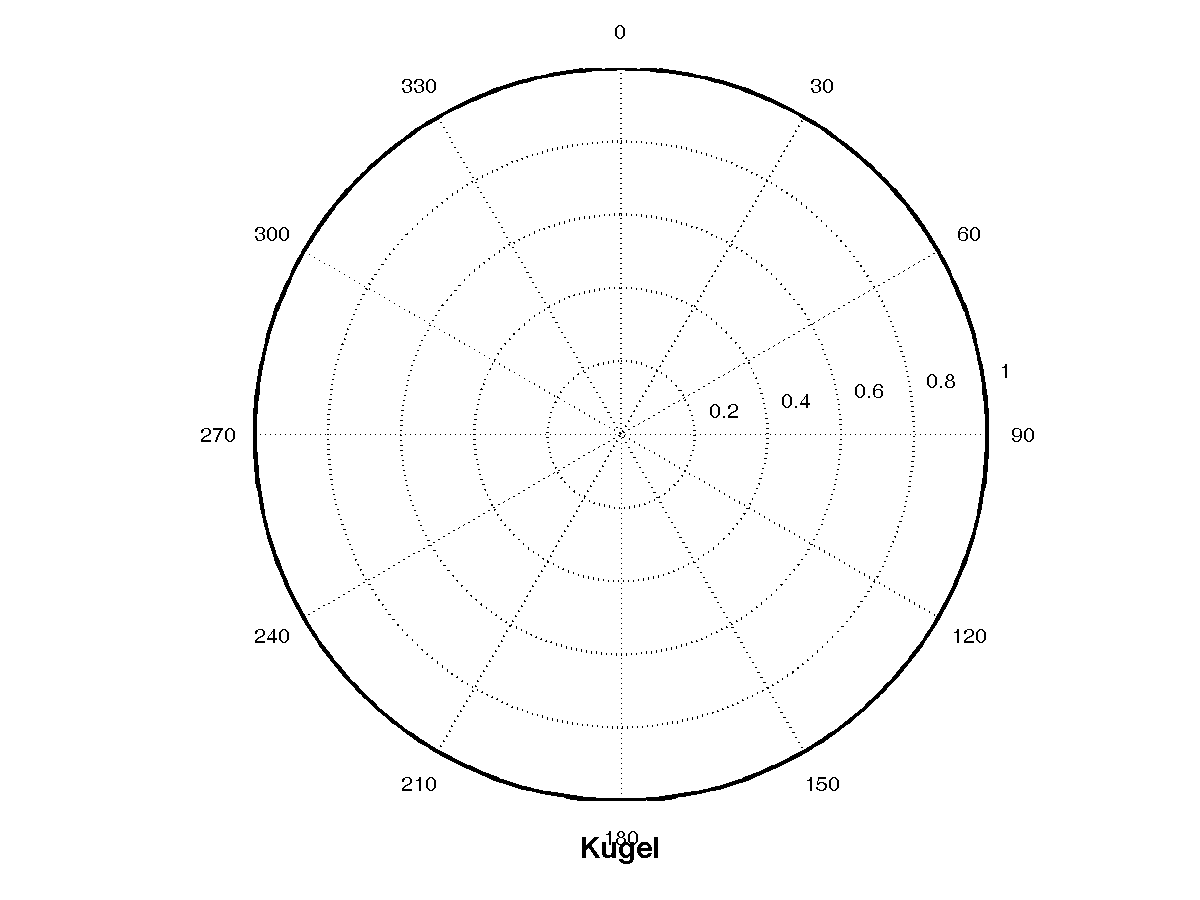
\includegraphics[scale=0.3]{Graph/n_rc_kugel}
			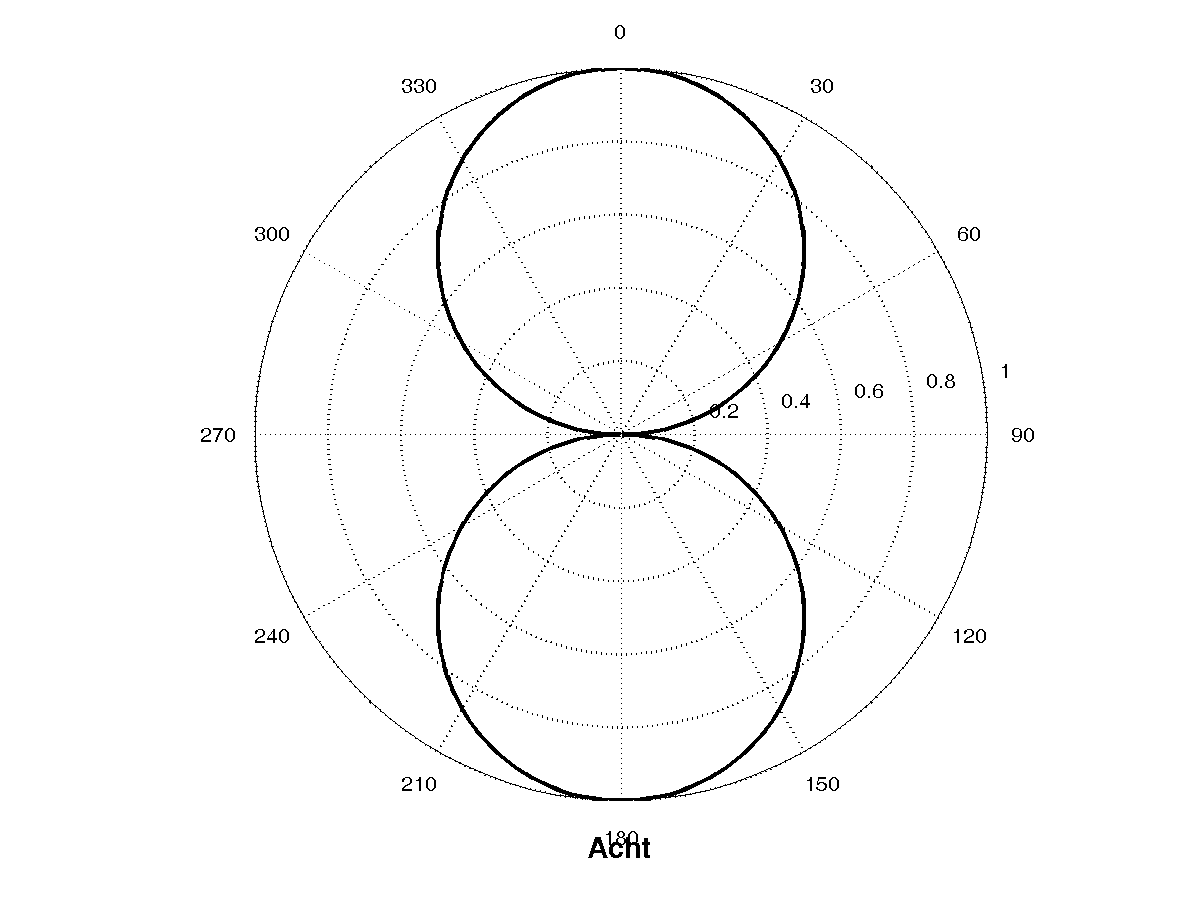
\includegraphics[scale=0.3]{Graph/n_rc_acht}
			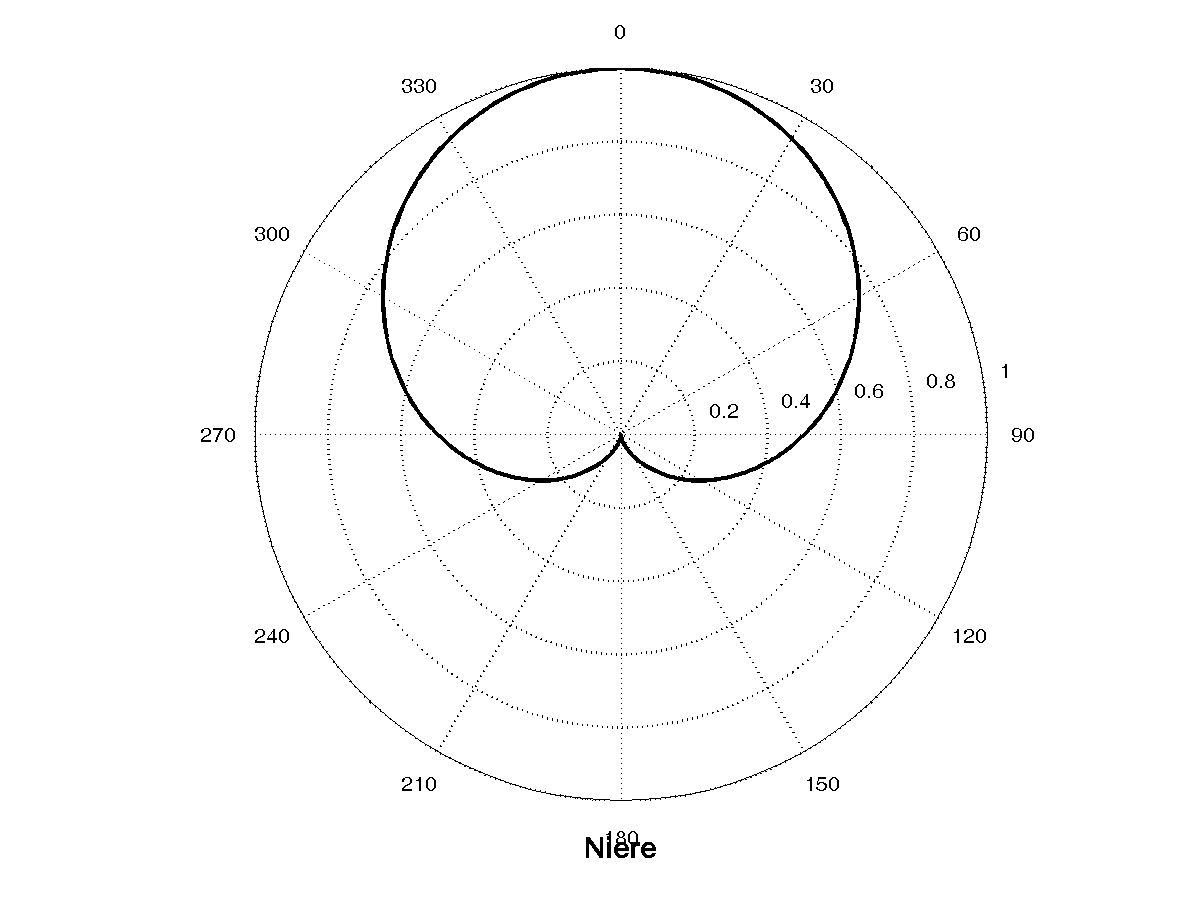
\includegraphics[scale=0.3]{Graph/n_rc_niere}
			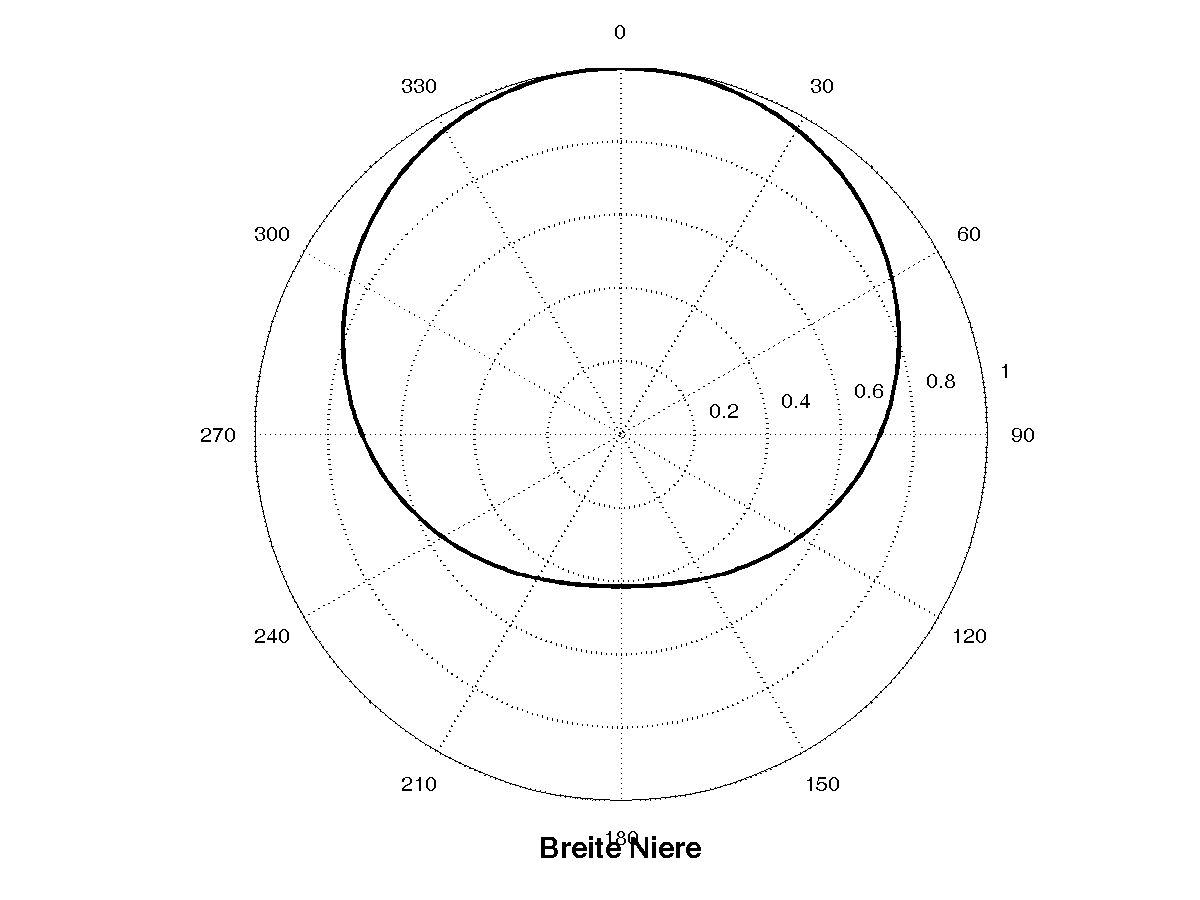
\includegraphics[scale=0.3]{Graph/n_rc_bniere}
			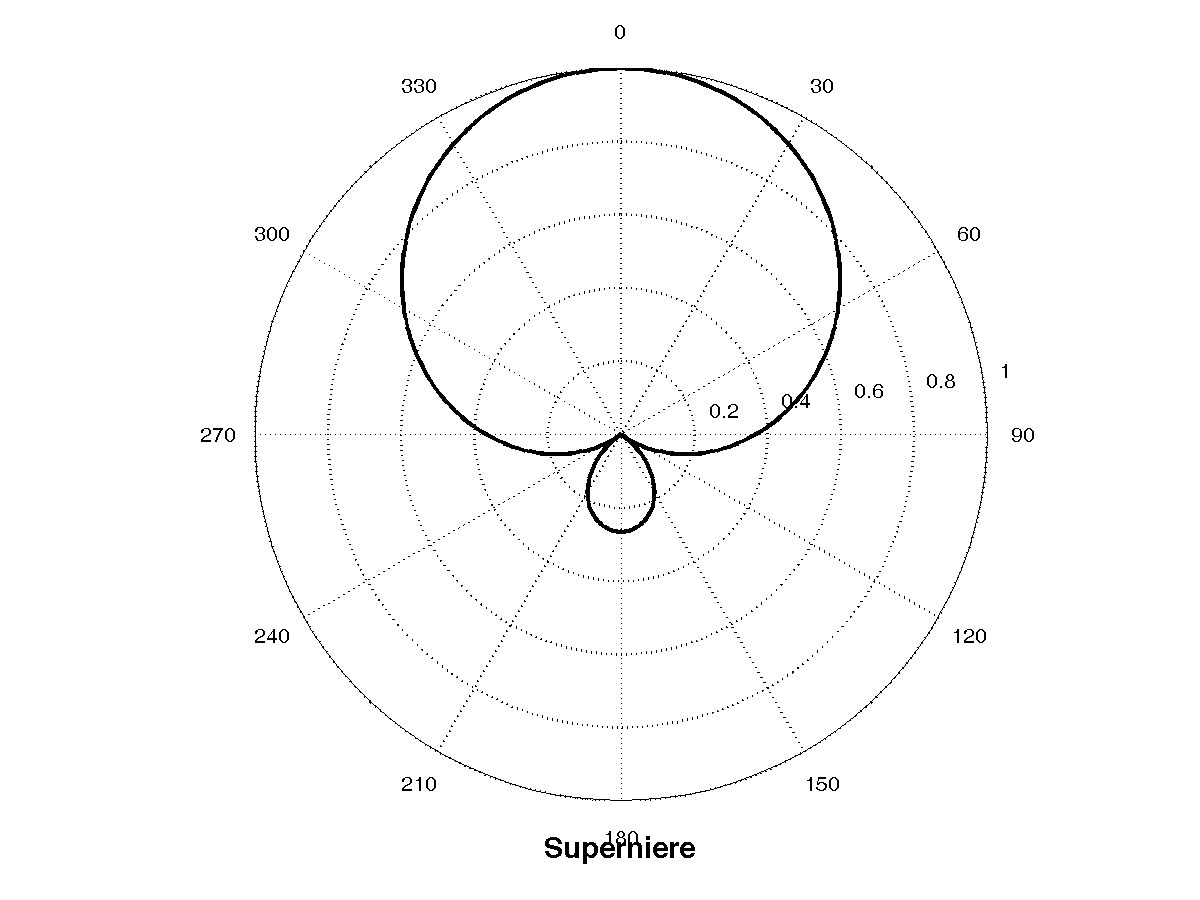
\includegraphics[scale=0.3]{Graph/n_rc_sniere}
			\includegraphics[scale=0.3]{Graph/n_rc_hniere}
			\caption[Mikrophon-Richtcharakteristiken]{Richtcharakteristiken von Mikrophonen; oben Kugel, Niere und Acht, unten Breite Niere, Superniere und Hyperniere} \label{fig:rc}
			\end{center}
		\end{figure}
Technisch ausgedr�ckt wird der Feld�bertragungsfaktor f�r jeden Einfallswinkel aufgetragen. Setzt man an einer bestimmten Einfallsrichtung den Feld�bertragungsfaktor ins Verh�ltnis zum Feld�bertragungsfaktor der $0^\circ$-Bezugsrichtung, so erh�lt man den sogenannten \bld{Richtungsfaktor}\index{Richtungsfaktor|bld} $\Gamma$ des Mikrophons f�r diesen Einfallswinkel $\theta$. Der 20-fache Logarithmus des Richtungsfaktors ist das \bld{Richtungsma�}\index{Richtungsma�|bld}. Somit ist das Richtungsma� f�r die Bezugsrichtung immer $0dB$.

Die dargestellten Richtcharakteristiken sind idealisiert. In den Datenbl�ttern realer Mikrophone kann man deutliche Abweichungen zu den idealen Kurven sehen. Insbesondere spielt hier die Frequenzabh�ngigkeit der Richtcharakteristik eine gro�e Rolle. So f�hren Reflexions- und Beugungseffekte am Mikrophonkorpus i.a. dazu, da� die Empfindlichkeit des Mikrophones sich ver�ndert. Eigentlich kugelf�rmige Richtcharakteristiken k�nnen so beispielsweise bei h�heren Frequenzen deutlich gerichtet werden. Aus diesem Grund werden von Mikrophonherstellern i.a. verschiedene Graphen f�r verschiedene Frequenzen angegeben.
	
Die Richtwirkung des Mikrophones wird teilweise auch durch einzelne Werte beschrieben, v.a. dem \bld{B�ndelungsgrad}\index{B�ndelungsgrad|bld} und dem \bld{B�ndelungsma�}\index{B�ndelungsma�|bld}. Der B�ndelungsgrad vergleicht die Richtcharakteristik des Mikrophons mit einer Kugelcharakteristik. Je geringer die Leistung des Raumschalls im Verh�ltnis zu der Raumschalleistung eines Mikrophons mit Kugelcharakteristik und dem gleichen Feld�bertragungsma� ist, desto h�her ist der B�ndelungsgrad. \\

	\bem{
	Mathematisch berechnet sich der B�ndelungsgrad $\gamma$ aus dem Richtungsfaktor $\Gamma$ in Abh�ngigkeit vom Einfallswinkel $\theta$:
	\begin{equation}
		\gamma = \frac{2}{\int_0^\pi{\Gamma^2\left(\theta\right)\sin\left(\theta\right)\;d\theta}}
		\label{eq:buendelung}
	\end{equation}
	}\end{quote}

Das B�ndelungsma� ist der 10fache Logarithmus des B�ndelungsgrades und ist dementsprechend $0$ f�r Mikrophone mit Kugelcharakteristik.
Auch einige andere, mit dem B�ndelungsgrad verwandte Gr��en werden manchmal angegeben:
\begin{itemize}
	\item	\bld{Vergr��erungsfaktor}\index{Vergr��erungsfaktor|bld} (auch \emp{(relativer) Abstandsfaktor} oder \emp{Distance Factor} (DSF)): dieser Wert gibt an, wie weit der Abstand des Mikrophons zur Schallquelle im Vergleich zur Kugelcharakteristik entfernt werden kann, so da� das Verh�ltnis von Direkt- und Diffusschall gleich bleibt. Der Vergr��erungsfaktor berechnet sich �ber die Quadratwurzel aus dem B�ndelungsgrad.
	\item	\bld{Random Energy Efficiency}\index{Random Energy Efficiency|bld} (REE): aufgenommener St�rschall im Verh�ltnis zur Kugelcharakteristik. Dieser Wert ist reziprok zum B�ndelungsgrad.
\end{itemize}
Abb. \ref{fig:bundelung} zeigt die verschiedene Ma�e B�ndelungsgrad, DSF und REE in der �bersicht.
    \begin{figure}[!hbt]
			\begin{center}
			\includegraphics[scale=0.5]{Graph/n_bundelung}
			\caption[Ma�e zur Beschreibung der Richtwirkung]{B�ndelungsgrad, DSF und REE f�r verschiedene Richtcharakteristiken} \label{fig:bundelung}
			\end{center}
		\end{figure}

\chaplink
\begin{itemize}
	\item Abschnitt \ref{chap:hallradius}
\end{itemize}
\end{quote}
	

	\subsubsection{Impulsverhalten}
	Auch wenn zwei unterschiedliche Mikrophone vergleichbare Kenndaten haben, k�nnen sie dennoch unterschiedlich klingen. Dies liegt dann meistens am unterschiedlichen \bld{Impulsverhalten}\index{Impulsverhalten|bld} der Mikrophone. Dabei wird nichts anderes als die Impulsantwort (vgl. Abschnitt \ref{chap:linsystem}) des Mikrophons gemessen. Je nach Mikrophon ist die Impulsantwort unterschiedlich lang und teilweise klanglich verf�rbt. Dies kann sich deutlich auf das Klangbild auswirken, mu� aber nicht unerw�nscht sein. 
	
%\subsection{Arbeitsprinzip}
%Geschwindigkeitsempf�nger vs. Elongationsempf�nger

\subsection{Mikrophontypen}
Praktisch alle gebr�uchlichen Studiomikrophone verf�gen �ber eine Membran, die von Bewegungen der Luftteilchen in Schwingung versetzt wird wie auch das menschliche Trommelfell. Abh�ngig davon, wie die Schwingungen in elektrische Signale umgewandelt werden spricht man von einem unterschiedlichen \bld{Arbeitsprinzip}\index{Arbeitsprinzip} des Mikrophons. Hier trennt man zwischen den \bld{Elongationsempf�ngern}\index{Elongationsempf�nger}, bei denen die erzeugte elektrische Spannung proportional zur Auslenkung der Membran ist, und den \bld{Geschwindigkeitsempf�ngern}\index{Geschwindigkeitsempf�nger}, bei denen diese Spannung proportional zur Geschwindigkeit der Membran ist. Im folgenden sollen die beiden wichtigsten Vertreter dieser beiden Gattungen eingef�hrt werden: das Kondensatormikrophon als bekanntester Elongationsempf�nger und das dynamische Mikrophon als dem verbreitetsten Geschwindigkeitsempf�nger.
	\subsubsection{Kondensatormikrophon}\index{Kondensatormikrophon}
	\paragraph{Mechanischer Aufbau\\}
	Die Gr��en, die im mechanischen Aufbaus des Kondensatormikrophons die Schwingungseigenschaften und damit den �bertragungsfrequenzgang beeinflussen k�nnen, sind in Abb. \ref{fig:membran} dargestellt. Die wichtigsten sind:
	\begin{itemize}
		\item	die Masse der Membran,
		\item	die Steife des Luftpolsters hinter der Membran, und 
		\item	die St�rke der Reibung an der Membranaufh�ngung.
	\end{itemize}
	In der Mechanik spricht man in diesem Fall von einem \emp{einfachen Schwinger}.
	
	        \begin{figure}[!hbt]
			\begin{center}
            \begin{picture}(100,30)

                %boxes
                \put(30,5){\framebox(4,20)}
                \put(23,25){\framebox(11,4)}
                \put(23,1){\framebox(11,4)}

								%membranaufh�ngung
								\put(23,6){\circle{2}}
								\put(23,24){\circle{2}}

                %lines vertical
                \put(23,7){\line(0,1){16}}
                
                %fill
                \put(30,5){\line(1,1){4}}
                \put(30,7){\line(1,1){4}}
                \put(30,9){\line(1,1){4}}
                \put(30,11){\line(1,1){4}}
                \put(30,13){\line(1,1){4}}
                \put(30,15){\line(1,1){4}}
                \put(30,17){\line(1,1){4}}
                \put(30,19){\line(1,1){4}}
                \put(30,21){\line(1,1){4}}
                
                \put(23,28.5){\line(1,0){11}}
                \put(23,28){\line(1,0){11}}
                \put(23,27.5){\line(1,0){11}}
                \put(23,27){\line(1,0){11}}
                \put(23,26.5){\line(1,0){11}}
                \put(23,26){\line(1,0){11}}
                \put(23,25.5){\line(1,0){11}}
                
                \put(23,4.5){\line(1,0){11}}
                \put(23,4){\line(1,0){11}}
                \put(23,3.5){\line(1,0){11}}
                \put(23,3){\line(1,0){11}}
                \put(23,2.5){\line(1,0){11}}
                \put(23,2){\line(1,0){11}}
                \put(23,1.5){\line(1,0){11}}
                

                %text
                \put(39,24){\vector(-2,-1){12}}
                \put(40,24){\footnotesize{\shortstack[l]{federndes Luftpolster}}}
                \put(17,8){\vector(1,1){6}}
                \put(3,5){\footnotesize{\shortstack[l]{Membran}}}

                \put(5,24){\vector(1,0){16}}
                \put(-11,20){\footnotesize{\shortstack[l]{reibende\\ Membranaufh�ngung}}}


            \end{picture}
			\end{center}
			\caption[mechanischer Mikrophon-Aufbau]{mechanischer Aufbau eines Mikrophons}\label{fig:membran}
        \end{figure}

	Die Eigenschaften bei der Bewegung der Mikrophonmembran werden daher ma�geblich von folgenden Kr�ften bestimmt:
	\begin{itemize}
		\item	$F_m$: die Kraft, um die Membranmasse zu beschleunigen/in Bewegung zu setzen
		\item $F_r$: die D�mpfungs- oder Reibungskraft
		\item $F_s$: die Kraft, mit der die Steife des Lufpolsters die Schwingung beeinflu�t
	\end{itemize}
	Die Kraft, die das System von au�en in Bewegung setzt, mu� gleich der Summe dieser drei Kr�fte sein:
	\begin{equation}\label{eq:F}
		F = F_m + F_r + F_s
	\end{equation}
	
	Aus dieser Gleichung l��t sich die in Abb. \ref{fig:x_vs_F} dargestellte frequenzabh�ngige Membranauslenkung in Abh�ngigkeit der Membranmasse $m$, der D�mpfungskonstante $r$ und der Federkonstante $s$ herleiten. Das Kondensatormikrophon als Elongationsempf�nger ist direkt von der Auslenkung der Membran abh�ngig, daher kann man bei der dargestellten Kurve von der �bertragungsfunktion des mechanischen Teils des Kondensatormikrophons sprechen.
    \begin{figure}[!hbt]
			\begin{center}
			\includegraphics[scale=0.5]{Graph/n_mauslenkung}
			\caption[Mikrophonmembranauslenkung ]{�bertragungsfrequenzgang eines Elongationsempf�ngers\index{Elongationsempf�nger} in Abh�ngigkeit verschiedener D�mpfungswerte} \label{fig:x_vs_F}
			\end{center}
		\end{figure}
	
	\herl{
		In der Mechanik ergibt sich f�r Glg. (\ref{eq:F}) 
		\begin{eq}\label{eq:schwinger}
			F = m\ddot{x} + r\dot{x} + sx
		\end{eq}
		Jeder Punkt steht hierbei f�r eine Ableitung. Nimmt man eine cosinusf�rnige Membranauslenkung an und schreibt diese als komplexe Zahl, so erh�lt man (mit $ x = e^{j2\pi f t}$):
		\begin{eqnarray}
		F &=& -m(2\pi f)^2e^{j2\pi ft}+jr2\pi f e^{j2\pi ft} + s e^{j2\pi ft}\nonumber\\
		&=& \left(-m(2\pi f)^2 + jr2\pi f  + s\right)x
		\end{eqnarray}
	
	Die gesuchte �bertragungsfunktion ist die Auslenkung $x$ durch die Kraft $F$:
	\begin{eqnarray}
		x/F &=& \frac{1}{-m(2\pi f)^2 + jr2\pi f + s}\nonumber\\
		&=& \frac{1/s}{-\underbrace{\frac{m}{s}}_{:=(2\pi f_0)^2}(2\pi f)^2 + j\underbrace{\frac{r}{s}}_{:= \eta/(2\pi f_0)}2\pi f + 1}\nonumber\\
		&=& \frac{1/s}{1 - \frac{f^2}{f_0^2} + j\eta\frac{f}{f_0}}\label{eq:m_auslenkung}
	\end{eqnarray}
	Aus diesem Ergebnis f�r die Auslenkung der Memran lassen sich folgende Schl�sse ziehen:
	\begin{itemize}
		\item	ist die Anregungsfrequenz $f$ sehr klein ist ist die Membranauslenkung ausschlie�lich von der Federsteife $s$ abh�ngig und verl�uft n�herungsweise konstant
		\item	Es gibt eine Resonanz�berh�hung an der Stelle $2\pi f_0 = \sqrt{s/m}$.
		\item	Die St�rke der Resonanz�berh�hung h�ngt von $\eta = r2\pi f_0/s$, also inbesondere von der D�mpfung $r$ ab.
		\item	F�r Frequenzen oberhalb von $f_0$ spielt praktisch nur noch der quadratische Anteil des Nenners eine Rolle. Bei diesen Frequenzen nimmt der Frequenzgang also mit $12dB/Oct$ ab.
	\end{itemize}}\end{quote}
	Insgesamt hat der mechanische Aufbau eines Mikrophons also eine Tiefpa�charakteristik. Die verschiedenen Parameter werden zumeist wie folgt abgestimmt: die Masse der Membran $m$ m�glichst klein, um die Resonanzfrequenz $f_0$ steigen zu lassen und damit den linearen �bertragungsbereich zu vergr��ern, die Federsteife $s$ aus dem gleichen Grund m�glichst gro�, andererseits aber auch nicht zu gro�, um den �bertragungsfaktor nicht zu sehr zu verkleinern, und die D�mpfung r eher gro�, um die Resonanz�berh�hung breit und niedrig zu gestalten.

	\paragraph{Elektrischer Aufbau\\}
	Die Membran eines Kondensatormikrophones besteht aus Metall oder metallisiertem Kunststoff und stellt eine Elektrode eines Kondensators dar. Sie ist in geringem Abstand vor der elektrisch leitenden Gegenelektrode angeordnet. Jede Schwingung der Membran ver�ndert den Abstand zwischen beiden Elektroden und damit die Kapazit�t dieses Kondensators, was eine �nderung der Kondensatorspannung $U_C$ und eine �nderung der Ausgangsspannung $U_A$ zur Folge hat. Das prinzipielle Schaltbild des elektrischen Teils des Kondensatormikrophons ist in Abb. \ref{fig:elekt_condmik} dargestellt. 
	        \begin{figure}[!hbt]
			\begin{center}
            \begin{picture}(50,20)

                %Ausgangswiderstand
                \put(25.5,8){\framebox(2,5)}

								%membranaufh�ngung

                %Kondensator
                \put(10,10){\line(1,0){5}}
                \put(10,11){\line(1,0){5}}
                
                %Spannungsversorgung
                \put(19,2){\line(0,1){3}}
                \put(20,0){\line(0,1){7}}
                
                %Leitung
                \put(12.5,3.5){\line(1,0){6.5}}
                \put(20,3.5){\line(1,0){6.5}}
                \put(12.5,17.5){\line(1,0){14}}
                \put(12.5,3.5){\line(0,1){6.5}}
                \put(12.5,11){\line(0,1){6.5}}
                \put(26.5,3.5){\line(0,1){4}}
                \put(26.5,13.5){\line(0,1){4}}
                
                
                %fill
                %text
                \put(16,-1.5){\vector(1,0){7}}
                \put(18.5,-5){\footnotesize{\shortstack[c]{$U_0$}}}

                \put(8.5,7){\vector(0,1){7}}
                \put(4,9){\footnotesize{\shortstack[c]{$U_C$}}}

                \put(29,14){\vector(0,-1){7}}
                \put(30,9){\footnotesize{\shortstack[c]{$U_A$}}}

            \end{picture}
			\end{center}
			\caption[elektrischer Kondensatormikrophon-Aufbau]{elektrisches Prinzip des elektrostatischen Wandlers}\label{fig:elekt_condmik}
        \end{figure}
	 
	 Kondensatormikrophone ben�tigen eine Spannungsquelle $U_0$ zu Vorspannung. Diese wird oft \emp{Phantomspeisung}\index{Phantomspeisung} genannt.
			
			Der elektrische Aufbau des Kondensatormikrophons hat eine hochpa��hnliche �bertragungsfunktion.
			\herl{
				Die Kapazit�t $C$ des Kondensators ist abh�ngig vom Abstand der beiden Elektroden im Ruhezustand $d$ und der Membranauslenkung $x$, sowie von der Ruhekapazit�t $C_0$. Es gilt:
				\begin{eq}\label{eq:wechselcap}
					C = C_0\frac{1}{1-\frac{x}{d}}
				\end{eq}
				Die Ladung des Kondensators $Q$ ver�ndert sich ebenfalls mit Bewegung der Membran. Die Ladung entspricht der Summe von Ruheladung $Q_0$ und Wechselladung $q$. Es ergibt sich
				\begin{eq}\label{eq:wechsellad}
					Q = Q_0 + q
				\end{eq}
				Die Spannung �ber dem Kondensator $U_C$ ergibt sich aus dem Quotienten von Ladung und Kapazit�t. Mit den Glgn. (\ref{eq:wechselcap}) und (\ref{eq:wechsellad}) ergibt sich n�herungsweise:
				\begin{eqnarray}
					U_C &=& \frac{Q}{C}\nonumber\\
					&=& \frac{Q_0 + q}{C_0}\left(1-\frac{x}{d}\right)\nonumber\\
					&\approx& U_0\left(1-\frac{x}{d}\right) + \frac{q}{C_0}
				\end{eqnarray}
				Die Approximation ist g�ltig, wenn die Wechselladung $q<<Q_0$ und die Membranauslenkung $x<<d$.
			}\end{quote}
	\subsubsection{Dynamisches Mikrophon}\index{Dynamisches Mikrophon}
	\paragraph{Mechanischer Aufbau\\}
	Der mechanische Aufbau eines dynamischen Mikrophones entspricht dem des Kondensatormikrophons. Der entscheidende Unterschied ist jedoch, da� die gesuchte Ausgangsgr��e nicht wie bei dem Kondensatormikrophon die Membranauslenkung, sondern die Membrangeschwindigkeit $v$ ist. Daher ergibt sich f�r den mechanischen Aufbau des dynamischen Mikrophons ein anderer prinzipieller Frequenzgang, der Abb. \ref{fig:v_vs_F} dargestellt ist.
    \begin{figure}[!hbt]
			\begin{center}
			\includegraphics[scale=0.5]{Graph/n_mgeschw}
			\caption[Mikrophonmembrangeschwindigkeit]{�bertragungsfrequenzgang eines Geschwindigkeitsempf�ngers\index{Geschwindigkeitsempf�nger} in Abh�ngigkeit verschiedener D�mpfungswerte} \label{fig:v_vs_F}
			\end{center}
		\end{figure}
	
	\herl{	
	Da sich die Geschwindigkeit eines K�rpers aus der zeitlichen Ableitung des Ortes (in diesem Fall also der Membranauslenkung) ergibt, mu� die erhaltene Gleichung (\ref{eq:m_auslenkung}) zeitlich abgeleitet werden. Wie schon bei Glg. (\ref{eq:schwinger}) resultiert eine Ableitung in einer Multiplikation mit $j2\pi f$. Der resultierende Frequenzgang ist also
	\begin{eq}
		v/F =  \frac{j2\pi f/s}{1 - \frac{f^2}{f_0^2} + j\eta\frac{f}{f_0}}
	\end{eq}
	Der f�r Frequenzen kleiner der Resonanzfrequenz steigt die Membrangeschwindigkeit mit $6dB/Oct$ an, f�r gr��ere f�llt sie ebenfalls mit $6dB/Oct$. Da der in Abb. \ref{fig:v_vs_F} dargestellte �bertragungsfrequenzgang keinen linearen Teil mehr aufweisen kann, liegt es nicht mehr im Interesse des Entwicklers, die Resonanz hoch abzustimmen. Vielmehr wird die Resonanz nun in die Mitte des Frequenzbereichs gelegt und m�glichst stark ged�mpft, um den Frequenzgang zu linearisieren.
	}\end{quote}

	\paragraph{Elektrischer Aufbau\\}
	
	\subsubsection{Andere Mikrophontypen}

\subsection{Bauform}
	\subsubsection{Druckempf�nger}
	\subsubsection{Druckgradientenempf�nger}
	\subsubsection{Mischformen}
	\herl{
		Die Funktion des Richtungsfaktors bei f�r gemischte Charakteristiken lautet $\Gamma(\theta) = A + B\cos(\theta)$ mit A: Anteil der Kugelcharakteristik und B: Anteil der Achter-Charakteristik, wobei $A+B = 1$. Eingesetzt in Gleichung (\ref{eq:buendelung}) ergibt sich somit:
		\begin{equation}
			\gamma = \frac{2}{\int_0^\pi{\left(A + B\cos(\theta)\right)^2\sin\left(\theta\right)\;d\theta}}
		\end{equation}
		F�r das Integral im Nenner ergibt sich
		\begin{eqnarray}
			&\int_0^\pi{A^2\sin(\theta)\;d\theta} + \int_0^\pi{B^2\underbrace{\cos^2(\theta)}_{=\frac{1}{2}\left(1 + \cos(2\theta)\right)}\sin(\theta)\;d\theta} + \int_0^\pi{2ABcos(\theta)\sin(\theta)\;d\theta} &= \nonumber\\
			&\left[-A^2\cos(\theta)\right]_0^\pi + \frac{B^2}{2}\left(\int_0^\pi{\sin(\theta)\;d\theta} + \int_0^\pi{\underbrace{\cos(2\theta)\sin(\theta)}_{\frac{1}{2}\left(\sin(-\theta) + \sin(3\theta)\right)}\;d\theta} \right) + \left[AB\sin^2(\theta)\right]_0^\pi&=\nonumber\\
			&\left[-A^2\cos(\theta)\right]_0^\pi + \frac{B^2}{2}\left[-\cos(\theta)-\frac{1}{2}\cos(-\theta)-\frac{1}{6}\cos(3\theta)\right]_0^\pi + \left[AB\sin^2(\theta)\right]_0^\pi&=\nonumber\\
			&\left[-\left(A^2 + \frac{3B^2}{4}\right)\cos(\theta) - \frac{B^2}{12}\cos(3\theta)\right]_0^\pi &= \nonumber\\
			&2A^2 + \frac{2B^2}{3}\nonumber
		\end{eqnarray}
		
		Daraus folgt f�r den B�ndelungsgrad:
		\begin{equation}
			\gamma = \frac{1}{A^2 + \frac{B^2}{3}}
		\end{equation}
	}\end{quote}
	\subsubsection{Andere Bauformen}

\section{Lautsprecher}
akustischer Kurzschlu�, Lautsprecherzeile

\section{Zusammenfassung}

\section{Aufgaben}
\begin{enumerate}
	\item warum 12dB/oct bei Auslenkungs�bertragungsfreuenzgang?
\end{enumerate}

\nocite{wuttke, sank, goerne, bore}
 %
	\chapter{Digitaltechnik}
\thispagestyle{empty}

Die Digitaltechnik und die digitale Signalverarbeitung stellen in den meisten Studios die wichtigsten Komponenten des Tonstudioalltags. Dieses Kapitel gibt eine Einf�hrung in die Digitaltechnik und ein �bersicht �ber die verschiedensten mit Tontechnik oder Audiosignalverarbeitung verkn�pften Applikationen.


\section{Bin�re Zahlendarstellung}

	Digitale Systeme arbeiten nicht mit der uns gel�ufigen dezimalen Zahlendarstellung, sondern mit der sogenannten \bld{bin�ren Zahlensdarstellung}\index{Zahlendarstellung!bin�re}. Hervorstechendstes Merkmal dieses Systems ist, da� es ausschlie�lich auf zwei Ziffern basiert: $0$ und $1$.
	
	Die sogenannte \bld{Wortbreite}\index{Wortbreite} $W$ eines digitalen Systems besagt, wie viele solcher einzelnen Ziffern, die im folgenden \emp{Bits} genannt werden, zu einem Wort und damit zu einer Zahl zusammengef�gt werden. Bei einer Wortbreite von $16bit$, wie sie auf einer CD zu finden ist, bilden somit immer 16bit eine Zahl bzw. einen Amplitudenwert. Jedes einzelne Bit kann zwei verschiedene Zust�nde annehmen, d.h. insgesamt k�nnen $2\cdot2\cdot2\cdot\dots\cdot2\cdot2\cdot2 = 2^{16} = 65536$ verschiedene Zahlen dargestellt werden.
	
	Die dargestellte Zahl berechnet sich mit Hilfe von Zweierpotenzen: beispielsweise steht die bin�re Zahl $1001\,1011$ mit der Wortbreite $8bit$ f�r die dezimale Zahl $1\cdot2^7 + 0\cdot2^6 +0\cdot2^5 +1\cdot2^4 +1\cdot2^3 +0\cdot2^2 +1\cdot2^1 +1\cdot2^0 = 155$. Eine �nderung an der Stelle mit der h�chsten Potenz (links) f�hrt die gr��ten Ver�nderungen herbei, daher wird dieses Bit das \emp{Most Significant Bit (MSB)}\index{Most Significant Bit} genannt. Analog dazu f�hren �nderungen im Bit rechts die kleinsten �nderungen herbei; es wird \emp{Least Significant Bit (LSB)}\index{Least Significant Bit} genannt.
	
	Wie man sieht, lassen sich hier positive Zahlen von $0$ bis $255$ darstellen; im Falle von realen Audiosignalen bewegt sich die Amplitude des Signals um den Nullpunkt herum, d.h. es treten positive wie negative Amplitudenwerte auf. Dem wird dadurch Rechnung getragen, da� das MSB als eine Art Vorzeichen-Bit interpretiert wird; ist es $0$, so ist die Zahl positiv, im anderen Falle negativ. Das f�hrt bei $16bit$ Wortbreite zu dem Zahlenbereich $-32768$ bis $32767$. Die Aufteilung des Zahlenbereichs geschieht so, da� die positiven Zahlen genauso behandelt werden wie im vorzeichenlosen Fall, die negativen aber von der negativen Maximalamplitude hochgez�hlt werden. 
	\bsp{Es werden einige Beispiele in vorzeichenbehafteter Bin�rdarstellung mit 4 Bit Wortbreite gegeben:
		\begin{table}[!hbt]
			\begin{center}
				\begin{tabular}{c|c}
					\textbf{Bin�r} & \textbf{Dezimal}\\\hline
					$0001$			& $1$\\
					$0101$			& $5$\\
					$0111$			& $7$\\
					$1000$			& $-8$\\
					$1001$			& $-7$\\			
					$1111$			& $-1$\\			
				\end{tabular}
			\end{center}
		
			\caption[Bin�rwerte mit Vorzeichen]{Beispiel f�r vorzeichenbehaftete Bin�rwerte der Wortbreite 4 Bit}
			\label{tab:binaer_4bit}
		\end{table}
	}\end{quote}
\bem{
Der Bin�rwert eines vorzeichenbehafteten Signals nicht immer so einfach zu berechnen, wie man auf den ersten Blick meinen w�rde. Falls das Vorzeichenbit nicht gesetzt ist, kann die Zahl wie oben gezeigt berechnet werden; im Fall einer negativen Zahl m�ssen folgende Schritte durchgef�hrt werden:
\begin{enumerate}
	\item	die Bitfolge in ihre \emp{Komplement�rdarstellung} zu \emp{invertieren}, d.h. aus jeder $0$ eine $1$ zu machen und umgekehrt (Beispiel: $1001\,0111\,1100\,0001 \rightarrow 0110\,1000\,0011\,1110$, 
	\item	die resultierende positive Zahl wie oben erl�utert zu bestimmen (Beispiel: $0110\,1000\,0011\,1110$ entspricht der dezimalen Zahl $26686$),
	\item die Zahl mit einem negativen Vorzeichen zu versehen (Beispiel: $26686\rightarrow -26686$),
	\item $1$ von der Zahl zu subtrahieren (Beispiel: Endergebnis ist $-26687$)
\end{enumerate}}\end{quote}
	
\begin{sloppypar}
	\bem{Das erl�uterte Zahlenformat kann nur ganzzahlige Werte darstellen, es wird \bld{Festkommaformat}\index{Festkommaformat} (auch Fixed-Point-Format) genannt. Gerade im Audiobereich wird aber zum Teil auch mit einem anderen Format gearbeitet, dem sogenannten \bld{Flie�kommaformat}\index{Flie�kommaformat} (auch Floating-Point-Format oder Gleitkommaformat). Hier werden nur Nachkommastellen und ein Exponent abgespeichert. Der Vorteil dieses Formats f�r Audiobearbeitung ist, da� sehr kleine Zahlen sehr genau dargestellt werden k�nnen, sehr gro�e Zahlen hingegen ungenauer. Dies entspricht dem menschlichen H�rverm�gen recht gut. \\
	Das Floating-Point-Format wird im allgemeinen bei der Audiobearbeitung auf dem Computer und in einigen Hardwaresystemen verwendet. Zur �bertragung und Speicherung findet es normalerweise keinen Einsatz.
	}\end{quote}
\end{sloppypar}
	
\section{Digitalisierung eines Analogsignals}	
\subsection{Abtastung}\index{Abtastung}\label{chap:sampling}
Wenn wir den Verlauf einer Spannung oder des Schalldrucks betrachten, sehen wir \emp{kontinuierliche} Ver�nderungen des Signals �ber der Zeit. Solche kontinuierlichen Ver�nderungen kennzeichnen \emp{analoge} Signale. Wir k�nnen uns einen kurzen Zeitabschnitt betrachten und immer weiter hineinzoomen, ohne da� der Verlauf des Signals jemals unterbrochen wird. Ein solcher unterbrechungsfreier Zeitverlauf ist in der Digitaltechnik nicht darstellbar, da hierzu unendlich viele Punkte dargestellt werden m��ten. Stattdessen wird das analoge Signal in bestimmten Zeitabst�nden abgetastet und es werden nur die einzelnen Amplitudenwerte zum Abtastzeitpunkt gespeichert. Die Frequenz dieser Abtastung wird \bld{Abtastrate}\index{Abtastrate} (englisch: \bld{Sample Rate}) genannt, ihre Einheit ist nat�rlich [$H\!z$]. Abbildung \ref{fig:sampling} zeigt einen kleinen Ausschnitt eines kontinuierlichen (analogen) Signals und die resultierende abgetastete Folge.

    \begin{figure}[!hbt]
			\begin{center}
			\includegraphics[scale=0.5]{Graph/sampling}
			\caption[Abtastung eines analogen Signals]{Vergleichende Darstellung eines kontinuierlichen und eines abgetasteten Signalverlaufs, oben: kontinuierlicher Zeitverlauf, unten entsprechender abgetasteter Zeitverlauf} \label{fig:sampling}
			\end{center}
		\end{figure}

\subsubsection{periodisches Spektrum}
	Eine wichtige Eigenschaft der Abtastung l��t sich an einem Beispiel veranschaulichen; dazu betrachten wir mehrere Sinusschwingungen, die mit einer Frequenz von $6k\!Hz$ abgetastet werden. Die Originalsignale und die abgetasteten Signale f�r die Frequenzen $1k\!Hz$, $7k\!Hz$ und $13k\!Hz$ sind in Abb. \ref{fig:periodic_sample} dargestellt, w�hrend die Abb. \ref{fig:periodic_sample2} die Originalsignale und abgetasteten Signale f�r die Frequenzen $1k\!Hz$, $5k\!Hz$, $11k\!Hz$ und $17k\!Hz$ zeigt.
    \begin{figure}[!hbt]
			\begin{center}
			\includegraphics[scale=0.5]{Graph/periodic_sample}
			\caption[Abtastung von Sinusschwingungen unterschiedlicher Frequenz (1)]{Darstellung von analogem und abgetastetem Zeitverlauf von Sinusschwingungen der Frequenzen $1k\!Hz$, $7k\!Hz$ und $13k\!Hz$, die Abtastfrequenz ist $6kH\!z$; oben: kontinuierlicher Zeitverlauf, unten entsprechender abgetasteter Zeitverlauf} \label{fig:periodic_sample}
			\end{center}
		\end{figure}
    \begin{figure}[!hbt]
			\begin{center}
			\includegraphics[scale=0.5]{Graph/periodic_sample2}
			\caption[Abtastung von Sinusschwingungen unterschiedlicher Frequenz (2)]{Darstellung von analogem und abgetastetem Zeitverlauf von Sinusschwingungen der Frequenzen $1k\!Hz$, $5k\!Hz$, $11k\!Hz$ und $17k\!Hz$, die Abtastfrequenz ist $6kH\!z$; oben: kontinuierlicher Zeitverlauf, unten entsprechender abgetasteter Zeitverlauf} \label{fig:periodic_sample2}
			\end{center}
		\end{figure}

Abb. \ref{fig:periodic_sample} zeigt deutlich, da� die abgetasteten Signale bei diesen bestimmten Frequenzen identisch sind. Die abgetasteten Signal aus Abb. \ref{fig:periodic_sample2} sind zwar nicht identisch, haben aber die gleiche Frequenz und Amplitude, lediglich eine andere Phasenlage. Mit Hilfe dieser Beispiele ist man einer der wichtigsten Eigenschaften abgetasteter Signale auf der Spur, die lautet: \bld{die Spektren abgetasteter Signale sind periodisch mit der Abtastfrequenz}.

\herl{Ohne zu sehr ins mathematische Detail gehen zu wollen, l��t sich der Weg der Herleitung wie folgt beschreiben: die Abtastung eines Signals l��t sich darstellen als die Multiplikation des analogen Signals mit einem Signal, das genau an den Abtastwerten den Wert $1$ hat und an allen anderen Stellen den Wert $0$. Der Verlauf dieses Abtastsignals erinnert an einen Kamm, die Abst�nde der einzelnen Z�hne (\glqq$1$\grqq) des Kamms entsprechen dem Abtastintervall. Es l��t sich nun zeigen, da� die Frequenztransformation eines solchen Signals ebenfalls wie solcher Kamm aussieht, wobei der Abstand der Z�hne dieses Kamms nun der Abtastfrequenz entspricht. In Abschnitt \ref{chap:faltung} wurde darauf hingewiesen, da� eine Multiplikation zweier Signale im Zeitbereich einer Faltung der Frequenzdarstellungen dieser Signale entspricht. Es wird nun also das Spektrum des analogen Signals gefaltet mit dem kammf�rmigen Signal. Diese Faltung f�hrt dazu, da� das Spektrum des analogen Signals periodisch mit der Abtastfrequenz wieder auftaucht.
}\end{quote}

	\subsubsection{Abtasttheorem und Aliasing}
	Aus der Periodizit�t des Spektrums des abgetasteten Signals folgt eine wichtige Eigenschaft; die (hohen) Frequenzen der periodischen Spektren k�nnen sich �berlappen. Tun sie dies, so l��t sich nicht mehr unterscheiden, ob es sich um Frequenzen des Originalspektrums handelt oder um  hineingespiegelte Frequenzen. Es zeigt sich, da� sich die periodischen Spektren nicht �berlappen, wenn die Bandbreite des Signals kleiner als die halbe Abtastfrequenz ist. Dies ist das sogenannte \bld{Abtasttheorem}\index{Abtasttheorem}. Wird es nicht eingehalten (die sog. \emp{Unterabtastung}\index{Unterabtastung}, so entstehen \glqq Spiegelfrequenzen\grqq, die sehr unangenehm klingen k�nnen. Dieser Effekt wird \bld{Aliasing}\index{Aliasing} genannt. Aus diesem Grund befindet sich vor jedem AD-Wandler ein Tiefpa�filter, der (m�glichst) alle Frequenzanteile oberhalb der halben Abtastfrequenz herausfiltert und somit die Einhaltung des Abtasttheorems gew�hrleistet. Dieses Filter wird \emp{Antialiasingfilter}\index{Antialiasingfilter} genannt. Die G�te dieses Filters kann gro�en Einflu� auf die Wandlerg�te haben (siehe Abschnitt \ref{chap:rec_sample}).
	\bem{
	Ein anschauliches Beispiel einer Unterabtastung im visuellen findet man in vielen Westernfilmen. Die Speichenr�der einer Kutsche drehen sich mit der erwarteten Geschwindigkeit und Richtung, solange die Kutsche langsam f�hrt. �bersteigt die Speichengeschwindigkeit allerdings die halbe Abtastfrequenz der Kamera, so nimmt die wahrgenommene Geschwindigkeit des Rades wieder ab.}
	\end{quote}

	\subsubsection{Rekonstruktion des Signals}\label{chap:rec_sample}
	Zur Rekonstruktion des analogen Signals aus dem abgetasteten Signal mu� das abgetastete Signal tiefpa�gefiltert werden, um die periodischen Fortsetzungen des Spektrums \glqq herauszufiltern\grqq. Das Tiefpa�filter hat die Aufgabe, nur die Signalfrequenzen kleiner als die halbe Abtastfrequenz passieren zu lassen. Es wird \emp{Rekonstruktionsfilter}\index{Rekonstruktionsfilter} genannt. Theoretisch ist ein analoges Signal, welches unter Ber�cksichtigung des Abtasttheorems gesampelt wurde, ohne Verlust wieder rekonstruierbar. Leider gilt dies aber nur f�r den Fall, da� sowohl Antialiasingfilter als auch Rekonstruktionsfilter ideal sind, d.h. alle Frequenzen bis zur halben Abtastfrequenz ungehindert passieren lassen, aber keine Frequenzanteile oberhalb der halben Abtastfrequenz. Ein solches Filter ist praktisch nicht zu realisieren, sondern wird bei vorhandenen Wandlern nur mehr oder weniger gut approximiert.

	\bem{Als Entdecker des Abtasttheorem werden oft Nyquist oder Shannon genannt. Nyquist war wohl der erste, der das Abtasttheorem ca. 1930 ver�ffentlichte, w�hrend Shannon nach dem 2. Weltkrieg eine Generalisierung des Abtasttheorems publizierte. Daher werden als gleichbedeutend mit Begirff Abtasttheorem manchmal auch die Begriffe Nyquisttheorem und Shannontheorem verwendet.}
	\end{quote}
%        \begin{figure}[!hbt]
%			\begin{center}
%            \begin{picture}(50,90)

                %boxes
%                \put(0,50){\framebox(40,10){\footnotesize{Antialiasing-Filter}}}
%                \put(0,30){\framebox(40,10){\footnotesize{Abtastung}}}
%                \put(0,10){\framebox(40,10){\footnotesize{Rekonstruktions-Filter}}}

                %lines vertical
%                \put(20,70){\vector(0,-1){10}}
%                \put(20,50){\vector(0,-1){10}}
%                \put(20,30){\vector(0,-1){10}}
%                \put(20,10){\vector(0,-1){10}}
 
                %text
%                \put(23,63){\footnotesize{\shortstack[c]{kontinuierliches Eingangssignal}}}
%                \put(23,43){\footnotesize{\shortstack[c]{tiefpa�gefiltertes Eingangssignal}}}
%                \put(23,23){\footnotesize{\shortstack[c]{abgetastetes Eingangssignal}}}
%                \put(23,3){\footnotesize{\shortstack[c]{tiefpa�gefiltertes Eingangssignal}}}
%                
%            \end{picture}
%			\end{center}
%			\caption[Verarbeitungsschritte bei Abtastung]{Notwendige Verarbeitungsschritte vor und %nach der Abtastung eines Signals}\label{fig:flowchart_sampling}
%        \end{figure}


\subsection{Quantisierung}\index{Quantisierung}
Ebenso wie ein digitales Signal keinen kontinuierlichen Zeitverlauf haben kann (s. Abschnitt \ref{chap:sampling}), kann es auch keinen kontinuierlichen Amplitudenverlauf besitzen, da nur einzelne Werte abgespeichert werden k�nnen. Dies bedeutet, da� die Amplitude - ebenso wie die Zeit bei der Abtastung - in bestimmte Abschnitte oder besser Stufen eingeteilt werden mu�. Dieser Vorgang wird \bld{Quantisierung}\index{Quantisierung} genannt. Eine kontinuierlich steigende Amplitude wird durch den Quantisierungsvorgang auf eine Treppenfunktion abgebildet. Diese Treppenfunktion wird auch als Quantisierungskennlinie bezeichnet und ist in Abb. \ref{fig:quant} rechts dargestellt.
    \begin{figure}[!hbt]
			\begin{center}
			\includegraphics[scale=0.5]{Graph/quant}
			\caption[Quantisierungskennlinie]{links: Amplitudenkennlinie bei amplitudenkontinuierlicher �ber\-tragung, jeder Eingangsamplitudenwert wird auf den exakt gleichen Ausgangsamplitudenwert abgebildet; rechts: Amplitudenkennlinie bei Quantisierung mit 16 Amplitudenstufen, bestimmte Amplitudenbereiche der Eingangsamplitude werden auf einzelne feste Werte abgebildet} \label{fig:quant}
			\end{center}
		\end{figure}
Wie an dieser Abbildung veranschaulicht, ist das Prinzip der Quantisierung, bestimmte Amplitudenbereiche auf einzelne \emp{quantisierte} Werte abzubilden. Die Quantisierungskennlinie ist damit eine treppenf�rmige Funktion. Je mehr einzelne Stufen erlaubt werden, desto kleiner werden die Stufen und desto �hnlicher wird das quantisierte Signal dem originalen kontinuierlichen Signal. Die Anzahl der Stufen bestimmt die Zahl der zur Speicherung eines Wertes ben�tigten Bits. $16$ Stufen lassen sich mit $4$ Bit darstellen; im Fall der Abb. \ref{fig:quant} handelt es sich also um einen $4$-Bit-Quantisierer. Wortbreite\index{Wortbreite} eines digitalen Signals und Anzahl der Quantisierungsstufen sind also direkt ineinander �berzuf�hren: um ein digitales Signal der Wortbreite $16$ Bit zu erhalten, mu� die Anzahl der Stufen $65536$ betragen. Soll die Wortbreite voll ausgenutzt werden, so m�ssen Minimal- und Maximalamplitude (oder -spannung) des Signals und Eingangsminimal- und Maximalspannung des Quantisierers �bereinstimmen. Je geringer die Aussteuerung des Eingangssignals ist, desto gr��er wird der Quantisierungsfehler verglichen zum Eingangssignal. Andererseits mu� eine �bersteuerung des Quantisierers unter allen Umst�nden vermieden werden, da die �bersteuerungsartefakte, zu sehr unangenehmen Verzerrungen f�hren k�nnen.

\subsubsection{Quantisierungsfehler}
	Die Abtastung eines Signals ist theoretisch ohne Verluste r�ckg�ngig zu machen, bei der Quantisierung allerdings ist dies auch in der Theorie nicht m�glich. Bei jeder Quantisierung wird unvermeidlich ein Fehler gemacht, der sog. \bld{Quantisierungsfehler}\index{Quantisierungsfehler} $q$ (auch Quantisierungsrauschen\index{Quantisierungsrauschen}). Dieser berechnet sich aus der Differenz zwischen dem Originalsignal $x$ und dem quantisierten Signal $x_q$ f�r einen beliebigen Zeitwert $t$.
	\begin{equation}
		q(t) = x(t) - x_q(t)
	\end{equation}
Es wird i.a. davon gesprochen, da� dieser Fehler dem Signal hinzugef�gt wird; tats�chlich ergibt ja die Subtraktion von $x(t)-q(t)$ das quantisierte Signal $x_q(t)$. Abb. \ref{fig:quanterror} zeigt den Quantisierungsfehler eines mit $4$ Bit quantisierten optimal ausgesteuerten Sinussignals.
    \begin{figure}[!hbt]
			\begin{center}
			\includegraphics[scale=0.5]{Graph/quanterror}
			\caption[Quantisierungsfehler eines optimal ausgesteuerten Sinussignals]{links oben: das kontinuierliche Originalsignal; rechts oben: das mit einer Aufl�sung von $4$ Bit quantisierte Signal; unten: der dabei gemachte Quantisierungsfehler} \label{fig:quanterror}
			\end{center}
		\end{figure}
Es ist anschaulich klar, da� der Quantisierungsfehler kleiner wird, wenn die Zahl der Stufen bei gleichbleibender Maximalamplitude erh�ht wird, denn der Betrag der Amplitude des Quantisierungsfehlers kann maximal eine halbe Stufenh�he $\Delta$ betragen. Mit diesem Wissen l��t sich der (theoretische) Rauschabstand eines Quantisierers berechnen. Da die Stufenh�he $\Delta$ durch die Wortbreite $W$ des resultierenden digitalen Signals bestimmt wird, kann man den Rauschabstand $SNR$ direkt auf die Wortbreite des Signals zur�ckf�hren und gelangt zu der Beziehung:
\begin{equation}\label{eq:quanterror}
	SNR = 6.02\cdot W + const.\;\;[dB]
\end{equation}
Die Konstante $const.$ ist abh�ngig von Eingangssignal; sie ist f�r ein Sinussignal $1.76dB$ und f�r ein Sprach- bzw. Musiksignal im Bereich $-7$ bis $-8dB$. Als Daumenregel klingt die Gleichung (\ref{eq:quanterror}) so: \emp{Wird die Wortbreite eines Quantisierers um 1 Bit erh�ht, so gewinnt man 6dB Rauschspannungsabstand}.
\herl{
Die Maximalamplitude des Quantisierungsfehlers ist $\frac{\Delta}{2}$. Geht man davon aus, da� alle Amplitudenwerte zwischen den Maximalausschl�gen des Quantisierers gleichh�ufig vorkommen (das ist als N�herung erlaubt, wenn die Stufenanzahl gro� ist), so kann die Leistung des Quantisierungsfehlers berechnet werden mit
\begin{equation}
	\sigma_q^2 = \int^{\frac{\Delta}{2}}_{-\frac{\Delta}{2}}{\frac{1}{\Delta}x^2\,dx} = \frac{\Delta^2}{12}
\end{equation}
Der $SNR$ berechnet sich aus dem Quotienten von Signalleistung zu Fehlerleistung. Als Beispiel nehmen wir nun eine optimal ausgesteuerte Sinusschwingung. Die Amplitude entspricht daher der H�lfte der Zahl der Stufen $2^W$ multipliziert mit der Stufenh�he $\Delta$. Daraus folgt:
\begin{equation}
	\sigma_{Sinus}^2 = \int_0^{2\pi}{\left(Amplitude\cdot \sin(x)\right)^2\;dx}\frac{(Amplitude)^2}{2} = \frac{({2^W}\cdot\Delta)^2}{8}
\end{equation}
Somit ergibt sich f�r den Signalrauschabstand des Quantisierers:
\begin{eqnarray}
	SNR &=& 10\log\left(\frac{\sigma_{Sinus}^2}{\sigma_q^2}\right)\nonumber\\ 
	&=& 10\log\left(\frac{({2^W}*\Delta)^2\cdot 12}{8\cdot\Delta^2}\right)\nonumber\\
	&=& 10\log\left(2\right)\cdot 2\cdot W + 10\log\left(\frac{3}{2}\right)\nonumber\\
	&=& 6.02 \cdot W + 1.76\;\;[dB]\nonumber
\end{eqnarray}
}\end{quote}

\subsubsection{Oversampling}
Um die Qualit�t einer Digitalisierung zu verbessern, wird oftmals mit sog. \bld{Oversampling}\index{Oversampling} gearbeitet. Oversampling bedeutet, da� das Audiosignal mit einer h�heren Frequenz abgetastet wird als ben�tigt wird bzw. als am Ausgang des Wandlers auftritt. Es gibt v.a. zwei Gr�nde f�r diese �berabtastung. Der erste Grund ist die effiziente technische Realisierung: um maximale Audiobandbreite bis nah an die halbe Abtastfrequenz ohne aufwendiges Antialiasingfilter realisieren zu k�nnen, wird die Abtastrate so hochgesetzt, da� ein einfaches Antialiasingfilter gen�gt um das Abtasttheorem zu erf�llen. Anschlie�end wird das Signal im digitalen Bereich tiefpa�gefiltert, so da� es die Anforderungen des Abtasttheorems f�r die eigentlich gewollte Abtastfrequenz erf�llt.\\
Dieses Vorgehen hat einen erw�nschten Nebeneffekt, welcher der zweite Grund f�r die tempor�re Erh�hung der Abtastfrequenz ist: der Signal-Rauschabstand\index{Signal-Rauschabstand} (SNR) kann verbessert werden. Das ist zun�chst �berraschend, da die Abtastrate zun�chst nur die Bandbreite des digitalisierten Signals beeinflu�t, nicht den SNR. Zwei wichtige Eigenschaften bei der Digitalisierung f�hren jedoch zu einer Erkl�rung:
\begin{itemize}
	\item	Die Gesamtleistung des Quantisierungsrauschens ist unabh�ngig von der Abtastfrequenz.
	\item	Das Quantisierungsrauschen ist n�herungsweise wei�es Rauschen, das �ber die gesamte Bandbreite des Signals gleichm��ig verteilt wird.
\end{itemize}
Wenn also die Gesamtleistung des Quantisierungsfehlers gleich bleibt, obwohl die Abtastfrequenz erh�ht wird, dann wird bei Erh�hung der Abtastfrequenz die durchschnittliche Leistung in einem bestimmten Frequenzbereich sinken, da es sich �ber einen gr��eren Frequenzbereich erstrecken kann. Wendet man anschlie�end den oben angesprochenen digitalen Antialiasingfilter an, so wird der Anteil des Quantisierungsrauschen �ber der endg�ltigen halben Abtastfrequenz \glqq weggefiltert\grqq, und der SNR steigt. Man gewinnt mit solchen Oversamplingverfahren pro Frequenzverdopplung ca. $3dB$ Signal-Rauschabstand.

\subsubsection{Dither\index{Dither}}
Das Verh�ltnis bzw. der Signal-Rauschabstand des quantisierten Signals wird schlechter je geringer das Signal ausgesteuert wird. Doch eine schlechte Aussteuerung f�hrt nicht nur zu h�herem Rauschpegel, sondern kann einen weiteren Effekt haben - das Quantisierungsrauschen ist kein wei�es Rauschen mehr wie bei hohen Amplituden, sondern wird abh�ngig vom Eingangssignal Abbildung \ref{fig:3stepquant} zeigt ein mit drei Stufen quantisiertes Signal und dessen Quantisierungsfehler. Der hier eingef�hrte Quantisierungsfehler h�rt sich an wie sehr st�rende Verzerrungen und ist besonders deutlich bei niedriger Aussteuerung und tiefen Signalfrequenzen. Diese sind zwar bei hochaufl�senden Wandlern mit gro�em Dynamikumfang kaum mehr h�rbar, sollen aber bei niedriger aufl�senden Wandlern oder bei Wortbreitenkonvertierungen wie z.B. $24bit$ nach $16bit$ oder niedriger m�glichst vermieden werden. 
    \begin{figure}[!hbt]
			\begin{center}
			\includegraphics[scale=0.5]{Graph/3stepquant}
			\caption[Quantisierungsfehler bei einer 3-stufigen Quantisierung]{oben: Originalsignal, mitte: 3-stufig quantisiertes Signal, unten: Quantisierungsfehler} \label{fig:3stepquant}
			\end{center}
		\end{figure}
Eine naheliegende Idee ist nun, das Signal etwas \glqq analoger\grqq$\;$ zu machen, indem vor dem Quantisierungsproze� einfach ein Rauschen addiert wird. Dieses Rauschen wird \bld{Dither}\index{Dither} genannt. \\
Zun�chst naheliegend scheint die Annahme, dieses Rauschen m��te so stark sein, da� es die o.g. Verzerrungen akustisch verdeckt; das mu� aber \emp{nicht} der Fall sein. Vielmehr gen�gt ein schwaches Rauschen, das zu einer nicht mehr deterministischen, gleichbleibenden Abfolge der ausgew�hlten Quantisierungsstufen f�hrt, sondern zu einer eher zuf�lligen. Wenn beispielweise am Eingang eine Gleichspannung von $1.3mV$ anl�ge, der Quantisierer das Signal allerdings in $1mV$-Schritten quantisiert, dann wird das quantisierte Signal bei einem ungeditherten Eingang konstant bei $1mV$ liegen. Wird das Eingangssignal hingegen gedithert, so wird es manchmal bei $2mV$, h�ufiger bei $1mV$ und sehr selten bei anderen Quantisierungswerten liegen. Tats�chlich wird dann aber beim quantisierten ein Mittelwert von $1.3mV$ feststellbar sein, d.h. im Mittel ist die geditherte Quantisierung genauer, da beliebige Quantisierungswerte m�glich gemacht werden. Abbildung \ref{fig:ditherquant} zeigt das obige Beispiel mit einem hinzugef�gten Dithersignal. Abbildung \ref{fig:ditherquantfreq} zeigt die Spektren des quantisierten Signals und des gedithert quantisierten Signals.
    \begin{figure}[!hbt]
			\begin{center}
			\includegraphics[scale=0.5]{Graph/ditherquant}
			\caption[Quantisierungsfehler bei einer leicht geditherten Quantisierung]{oben: gedithertes Originalsignal, mitte: grob-stufig quantisiertes Signal, unten: Quantisierungsfehler bei gedithertem Eingang} \label{fig:ditherquant}
			\end{center}
		\end{figure}
    \begin{figure}[!hbt]
			\begin{center}
			\includegraphics[scale=0.5]{Graph/ditherfreq}
			\caption[Spektrum eines geditherten Signals]{Spektrum eines mit und ohne Dither quantisierten Signals; oben: ungedithert quantisiertes Signal, unten: gleichf�rmig gedithert quantisiertes Signal} \label{fig:ditherquantfreq}
			\end{center}
		\end{figure}
	\bsp{Die Wirkung des Dithering l��t sich leicht anhand eines Beispiels veranschaulichen. H�lt man sich eine Hand mit leicht ge�ffneten Fingern vor die Augen, so wird ein Gro�teil des Gesichtsfeldes von den Fingern abgedeckt, und nur durch die Zwischenr�ume l��t sich etwas erkennen. Bewegt man diese Hand allerdings sehr schnell, so lassen sich - wenn auch etwas undeutlich - auch die Bereiche erkennen, die zuvor von den Fingern verdeckt waren.}\end{quote}
	
	Die Erfahrung hat gezeigt, da� Ditheramplituden im Bereich der halben bis zur $1.5$-fachen Stufenbreite zu besten Ergebnissen f�hren.\\
	Das Ditherspektrum ist zumeist entweder wei� oder leicht hochpa�gefiltert. Eine Hochpa�filterung f�hrt in den meisten F�llen zu einer subjektiven Qualit�tsverbesserung, da die Rauschleistung etwas aus dem H�rbereich herausgeschoben wird.\\
	Ein wichtiger Aspekt des Ditherrauschens ist seine Amplitudendichteverteilung\index{Amplitudendichteverteilung} (ADV), d.h. die Wahrscheinlichkeit unterschiedlicher Signalwerte. Das \glqq reale\grqq$\;$ zur Amplitudendichteverteilung ist die H�ufigkeitsverteilung, die eine N�herung der ADV darstellt (vgl. Abschnitt \ref{chap:adv}). Wenn alle Signalwerte gleichh�ufig vorkommen, spricht man von gleichverteiltem Rauschen\index{Rauschen!gleichverteiltes} und die Amplitudendichteverteilung ist rechteckf�rmig. Man ist aber i.a. der Meinung, da� ein gleichverteiltes Rauschen nicht zu optimalen Dithering-Ergebnissen f�hrt, w�hrend ein dreieckf�rmig verteiltes Rauschen\index{Rauschen!dreieckf�rmig verteiltes} zu einem besseren H�reindruck f�hrt. Abbildung \ref{fig:dither} zeigt die Zeitverl�ufe und die Amplitudendichteverteilungen von gleich- und dreieckf�rmig verteiltem Rauschen.
    \begin{figure}[!hbt]
			\begin{center}
			\includegraphics[scale=0.5]{Graph/dither}
			\caption[Ditherformen]{Zeitverl�ufe (links) und Amplitudendichteverteilungen (rechts) von Rauschen; oben: gleichverteilt, unten: dreieckf�mig verteilt} \label{fig:dither}
			\end{center}
		\end{figure}
Teilweise kann man auch anders geformte Dither verwenden; z.B. gibt es h�ufig gau�f�rmige Rauschen. Eine gau�f�rmige Verteilung sieht glockenf�rmig aus.\\
Die Verwendung unterschiedlicher Ditherformen f�hrt auch zu unterschiedlichem Rauschpegel. Der eingef�gte Rauschpegel bewegt sich bei den o.g. Ditheramplituden zwischen $3$ und $6dB$.
\chaplink
\begin{itemize}
	\item Abschnitt \ref{chap:adv}
\end{itemize}
\end{quote}

\subsubsection{Noise-Shaping}
\begin{sloppypar}
\bld{Noise-Shaping}\index{Noise-Shaping} ist eine Methode, die Qualit�t eines Wandlers oder einer Wortbreitenkonvertierung zu erh�hen. Der Quantisierungsfehler, der bei normaler Quantisierung n�herungsweise ein wei�es Spektrum hat, wird spektral geformt. Idealerweise wird dabei die Rauschleistung von Frequenzbereichen hoher Geh�rempfindlichkeit (wie z.B. $2-4kH\!z$, vgl. Abschnitt \ref{chap:lautstaerke}) in Bereiche geringerer Empfindlichkeit verschoben (zumeist hohe Frequenzbereiche). Diese Frequenzverschiebung wird durch eine R�ckkopplung des Quantisierungsfehlers erreicht, je nachdem wieviele Koeffizienten diese R�ckkopplung hat, spricht man von Noise-Shaping verschiedener Ordnungen. Im Fall von Noise-Shaping erster Ordnung wird der Quantisierungsfehler festgestellt und vom darauffolgenden Sample subtrahiert. Dadurch entsteht eine Verschiebung des Quantisierungsfehlers hin zu h�heren Frequenzen. Komplexere Verschiebungen, die verschiedene Frequenzbereiche unterschiedlich gewichten, lassen sich nur mit Noise-Shaping h�herer Ordnung bewerkstelligen. Es ist nat�rlich ein naheliegender Gedanke, den Spektralverlauf des Quantisierungsrauschens so zu gewichten, da� er optimal der Ruheh�rschwelle angepa�t ist, ein es existieren in der Tat einige solche System auf dem Markt. Welche Systeme nun besser sind und welche schlechter, sollte aber mit kritischem Material (z.B. Ausklingvorg�nge) selbst getestet werden.
\end{sloppypar}
Noise-Shaping wird meistens in Zusammenhang mit Dither\index{Dither} verwendet, um unerw�nschte Effeke bei der R�ckkopplung des Quantisierungsfehlers zu vermeiden.

Wortbreitenkonvertierungen und damit auch Noise-Shaping sollten m�glichst nur einmal am Ende der Verarbeitungskette eingesetzt werden.
\chaplink
\begin{itemize}
	\item Abschnitt \ref{chap:filter}
\end{itemize}
\end{quote}


\subsection{Wandler}\label{chap:wandler}
\subsubsection{Analog-Digital-Wandler}
\subsubsection{Digital-Analog-Wandler}

\section{Digitale Filter}

	\bld{Digitale Filter}\index{Filter!digitale} lassen sich ausschlie�lich durch \glqq Verz�gerungsglieder\grqq$\;$ und gewichtete Addition realisieren. Das bedeutet, da� jeder einzelne Abtastwert um bestimmte Zeiten verz�gert wird, mit unterschiedlichen Faktoren multipliziert wird und mit anderen, ebenfalls verz�gerten und gewichteten Abtastwerten aufaddiert wird. Warum sich Filter auf diese Art realisieren lassen, verdeutlicht man sich am besten anhand von Beispielen. Zuvor sollen die verwendeten Bestandteile der Filtergraphen\index{Filtergraph} kurz erl�utert werden. Ein Pfeil zeigt immer die Richtung des Signalflusses an. Ein Kreis symbolisiert eine Rechenoperation: befindet sich ein $+$ im Kreis, so werden zwei Signale aufaddiert, befindet sich ein $x$ im Kreis, so wird das Signal mit der nebenstehenden Konstante (\emp{Filterkoeffizient}\index{Filterkoeffizient}) multipliziert. Ein K�stchen mit dem Inhalt $z^{-n}$ bedeutet, da� der eingehende Abtastwert um $n$ Abtasttakte verz�gert wird.
	
	\begin{quote}\footnotesize \textbf{Beispiel 1}\\ 
        \begin{figure}[!hbt]
			\begin{center}
            \begin{picture}(50,30)

                %boxes
                \put(25,5){\framebox(7,6){\footnotesize{$z^{-1}$}}}

                %lines horizontal
                \put(5,20){\vector(1,0){20}}
                \put(30,20){\vector(1,0){10}}
                \put(45,20){\vector(1,0){10}}
                
                \put(15,8){\vector(1,0){10}}
                \put(32,8){\vector(1,0){8}}

                %lines vertical
                \put(15,20){\line(0,-1){12}}
                \put(42.5,10.5){\vector(0,1){7}}
                
                %circles
                \put(27.5,20){\circle{5}} \put(26.5,19){{{x}}}
%                \put(42.5,20){\circle{5}} \put(41,19){{{+}}}
                \put(41,19){$\oplus$}
                \put(42.5,8){\circle{5}} \put(41.5,7){{{x}}}
                
                \put(15,20){\circle*{1}}

                %text
                \put(26,24){\footnotesize{\shortstack[c]{$1/2$}}}
                \put(46,5){\footnotesize{\shortstack[c]{$1/2$}}}

                \put(4,22){\footnotesize{\shortstack[c]{x(n)}}}
                \put(52,22){\footnotesize{\shortstack[c]{y(n)}}}

            \end{picture}
			\end{center}
			\caption[Filter Beispiel 1]{Filter Beispiel 1}\label{fig:digfil_bsp1}
        \end{figure}
        
        Hier wird jeder einzelne Abtastwert mit $0.5$ multipliziert und mit dem vorhergehenden, ebenfalls mit $0.5$ multiplizierten Abtastwert addiert. Eine hypothetische Samplefolge $x(n)=[1\;110\;51\;20\;30\;0]$ f�hrt also zu einem Ausgang $y(n)=[0.5\;55.5\;80.5\;35.5\;25\;15]$. Wie lassen sich nun die Eigenschaften eines solchen Filters bestimmen? Die Impulsantwort l��t sich einfach auf die gleiche Art bestimmen, wie das schon mit der Samplefolge geschehen ist. Als Eingangssignal dient dazu eine einzelne $1$ (ein \emp{Impuls}). Man erh�lt als Impulsantwort also $[0.5\;0.5]$.\\
        Der Frequenzgang l��t sich nat�rlich berechnen, f�r so ein einfaches Beispiel allerdings auch relativ einfach absch�tzen. Daf�r stellen wir uns am Eingang des Filters ein Sinussignal variabler Frequenz vor. Bei sehr tiefen Frequenzen wissen wir, da� sich aufeinanderfolgende Abtastwerte stark �hneln. Da am Ausgang des Filters der Mittelwert des aktuellen und des vorhergehenden Abtastwertes erscheint (aus diesem Grund hei�t ein solches Filter auch Moving-Average- (MA-)Filter), hat dieses Filter f�r tiefe Frequenzen kaum Auswirkungen. F�r h�here Eingangsfrequenzen unterscheiden sich aufeinanderfolgende Werte zunehmend, so da� das Filter d�mpfend auf das Signal wirkt. Ist das Eingangssignal des Filters im Grenzfall ein Sinussignal mit der halben Abtastfrequenz, so ist der Mittelwert zwischen zwei aufeinanderfolgenden Abtastwerten und damit auch der Ausgang des Filters immer $0$. Somit handelt es sich in diesem Beispiel um ein \emp{Tiefpa�filter}. 
        \begin{figure}[!hbt]
			\begin{center}
			\includegraphics[scale=0.5]{Graph/filter1}
			\caption[Impulsantwort und �bertragungsfunktion von Filter Bsp.1]{Impulsantwort, Betragsfrequenzgang und Phasenfrequenzgang von Beispielfilter Nr.1} \label{fig:filter1}
			\end{center}
		\end{figure}
		
		Abbildung \ref{fig:filter1} zeigt die Impulsantwort, den Betragsfrequenzgang und den Phasenfrequenzgang dieses Filters. Deutlich zu erkennen ist die Tiefpa�charakteristik, die allerdings erst bei sehr hohen Frequenzen deutlich zum Tragen kommt. Der Phasenfrequenzgang ist linear.

	\end{quote}


	\begin{quote}\footnotesize \textbf{Beispiel 2}\\ 
        \begin{figure}[!hbt]
			\begin{center}
            \begin{picture}(50,30)


                %boxes
                \put(25,5){\framebox(7,6){\footnotesize{$z^{-1}$}}}

                %lines horizontal
                \put(5,20){\vector(1,0){20}}
                \put(30,20){\vector(1,0){10}}
                \put(45,20){\vector(1,0){10}}
                
                \put(15,8){\vector(1,0){10}}
                \put(32,8){\vector(1,0){8}}

                %lines vertical
                \put(15,20){\line(0,-1){12}}
                \put(42.5,10.5){\vector(0,1){7}}
                
                %circles
                \put(27.5,20){\circle{5}} \put(26.5,19){{{x}}}
                \put(42.5,20){\circle{5}} \put(41,19){{{+}}}
                \put(42.5,8){\circle{5}} \put(41.5,7){{{x}}}
                
                \put(15,20){\circle*{1}}

                %text
                \put(26,24){\footnotesize{\shortstack[c]{$1/2$}}}
                \put(46,5){\footnotesize{\shortstack[c]{$-1/2$}}}

                \put(4,22){\footnotesize{\shortstack[c]{x(n)}}}
                \put(52,22){\footnotesize{\shortstack[c]{y(n)}}}

            \end{picture}
            \end{center}
            \caption[Filter Beispiel 2]{Filter Beispiel 2}\label{fig:digfil_bsp2}
        \end{figure}
        
        Dieses Filter gleicht dem aus Beispiel 1 bis auf eine kleine �nderung genau. Lediglich der Faktor im Verz�gerungsteil ist nun $-0.5$ statt $0.5$. Die Impulsantwort lautet dementsprechend $[0.5\;-0.5]$. Wie schon im Beispiel 1 l��t sich der Frequenzgang des Filters sch�tzen. F�r sehr tiefe Frequenzen mit �hnlichen aufeinanderfolgenden Abtastwerten ist der Ausgang des Filters stark ged�mpft. Sind die aufeinanderfolgenden Abtastwerte gleich, so ist der Ausgang des Filters $0$. Mit zunehmender Eingangsfrequenz nimmt auch die Amplitude des Ausgangs zu, bis er bei der halben Abtastfrequenz maximal wird. Es handelt sich also um ein \emp{Hochpa�filter}.
        
        \begin{figure}[!hbt]
			\begin{center}
			\includegraphics[scale=0.5]{Graph/filter2}
			\caption[Impulsantwort und �bertragungsfunktion von Filter Bsp.2]{Impulsantwort, Betragsfrequenzgang und Phasenfrequenzgang von Beispielfilter Nr.2} \label{fig:filter2}
			\end{center}
		\end{figure}
		
		Abbildung \ref{fig:filter2}, in der Impulsantwort, Betragsfrequenzgang und Phasenfrequenzgang des Filters gezeigt werden, best�tigt die Herleitung der Impulsantwort und des Betragsfrequenzgangs. Der Phasefrequenzgang ist wie in Beispiel 1 linear.
	\end{quote}

	\begin{quote}\footnotesize \textbf{Beispiel 3}\\ 
        \begin{figure}[!hbt]
			\begin{center}
            \begin{picture}(50,30)


                %boxes
                \put(25,5){\framebox(7,6){\footnotesize{$z^{-11}$}}}

                %lines horizontal
                \put(5,20){\vector(1,0){20}}
                \put(30,20){\vector(1,0){10}}
                \put(45,20){\vector(1,0){10}}
                
                \put(15,8){\vector(1,0){10}}
                \put(32,8){\vector(1,0){8}}

                %lines vertical
                \put(15,20){\line(0,-1){12}}
                \put(42.5,10.5){\vector(0,1){7}}
                
                %circles
                \put(27.5,20){\circle{5}} \put(26.5,19){{{x}}}
                \put(42.5,20){\circle{5}} \put(41,19){{{+}}}
                \put(42.5,8){\circle{5}} \put(41.5,7){{{x}}}
                
                \put(15,20){\circle*{1}}

                %text
                \put(26,24){\footnotesize{\shortstack[c]{$1/2$}}}
                \put(46,5){\footnotesize{\shortstack[c]{$1/2$}}}

                \put(4,22){\footnotesize{\shortstack[c]{x(n)}}}
                \put(52,22){\footnotesize{\shortstack[c]{y(n)}}}

            \end{picture}
            \end{center}
            \caption[Filter Beispiel 3]{Filter Beispiel 3}\label{fig:digfil_bsp3}
        \end{figure}
        
        Auch dieses Beispiel wei�t gro�e �hnlichkeit mit Beispiel 1 auf. Die Filterkoeffizienten sind identisch, das Verz�gerungsglied verz�gert hingegen nicht mehr nur um einen Abtasttakt, sondern um $11$. Wenn wir uns den Betragsfrequenzgang wie bei den obigen Beispielen herleiten, kommen wir zu dem Schlu�, da� immer eine ganz bestimmte Frequenz und deren ganzzahlige Vielfache unterdr�ckt werden. Es handelt sich also um ein \emp{Kammfilter}.
        
        \begin{figure}[!hbt]
			\begin{center}
			\includegraphics[scale=0.5]{Graph/filter3}
			\caption[Impulsantwort und �bertragungsfunktion von Filter Bsp.3]{Impulsantwort, Betragsfrequenzgang und Phasenfrequenzgang von Beispielfilter Nr.3} \label{fig:filter3}
			\end{center}
		\end{figure}
	
	Abbildung \ref{fig:filter2} zeigt die Impulsantwort, den Betragsfrequenzgang und den Phasenfrequenzgang des Filters. Auch wenn es nicht so aussieht, ist auch in diesem Beispiel die Phase linear, lediglich die Darstellung kann Vielfache von $\frac{\pi}{2}$ nicht von $\frac{\pi}{2}$ selbst unterscheiden.
	\end{quote}


	\begin{quote}\footnotesize \textbf{Beispiel 4}\\ 
        \begin{figure}[!hbt]
			\begin{center}
            \begin{picture}(80,30)
                %boxes
                \put(42.5,5){\framebox(7,6){\footnotesize{$z^{-1}$}}}

                %lines horizontal
                \put(10,20){\vector(1,0){5}}
                \put(20,20){\vector(1,0){7.5}}
                \put(32.5,20){\vector(1,0){37.5}}
                
                \put(42.5,8){\vector(-1,0){10}}
                \put(57.5,8){\vector(-1,0){8}}

                %lines vertical
                \put(57.5,20){\line(0,-1){12}}
                \put(30,10.5){\vector(0,1){7}}
                
                %circles
                \put(17.5,20){\circle{5}} \put(16.5,19){{{x}}}
                \put(30,20){\circle{5}} \put(28.5,19){{{+}}}
                \put(30,8){\circle{5}} \put(29,7){{{x}}}
                
                \put(57.5,20){\circle*{1}}

                %text
                \put(15,24){\footnotesize{\shortstack[c]{$0.1$}}}
                \put(23,3){\footnotesize{\shortstack[c]{$0.9$}}}

                \put(4,22){\footnotesize{\shortstack[c]{x(n)}}}
                \put(67,22){\footnotesize{\shortstack[c]{y(n)}}}

            \end{picture}
            \end{center}
            \caption[Filter Beispiel 4]{Filter Beispiel 4}\label{fig:digfil_bsp4}
        \end{figure}
        
        In dem vierten und letzten Beispiel liegt eine andere Filterstruktur vor: der Verz�gerungspfad ist nun r�ckgekoppelt, d.h. da� jeder Ausgangswert wieder gewichtet mit einem Eingangswert addiert wird. In den bisherigen Beispielen hatte im Gegensatz dazu der Ausgangswert keinen Einflu� auf den folgenden Ausgangswert. Die Impulsantwort wird aufgrund der R�ckkopplung niemals ganz abklingen (jedenfalls bei unendlicher Rechengenauigkeit), also unendlich ausgedehnt sein. W�re der Faktor im R�ckopplungszweig gr��er als $1$, so wird das Filter instabil und liefert immer gr��ere Werte.\\
        Der Amplitudenfrequenzgang dieses Filters l��t sich anschaulich nicht mehr so leicht herleiten wie in den obigen Beispielen. Wir sehen allerdings, da� der R�ck\-kopplungs\-zweig st�rker den Ausgangswert bestimmt als der Eingang des Filters. Ver�ndert sich also der Eingang des Filters nicht oder nur sehr langsam, so wird der Ausgang des Filters dem Eingang �hnlich sein. �ndert sich der Eingang hingegen schnell, so werden sich diese �nderungen nur wenig Auswirkungen auf den Ausgang haben. Also liegt die Vermutung nahe, da� es sich in diesem Beispiel wiederum um ein \emp{Tiefpa�filter} handelt. Abbildung \ref{fig:filter4} best�tigt diese Annahme. Der Phasengang ist nicht linear, der Betragsfrequenzgang dieses Tiefpa�filters unterscheidet sich deutlich von dem aus Beispiel $1$.
        
        \begin{figure}[!hbt]
			\begin{center}
			\includegraphics[scale=0.5]{Graph/filter4}
			\caption[Impulsantwort und �bertragungsfunktion von Filter Bsp.4]{Impulsantwort, Betragsfrequenzgang und Phasenfrequenzgang von Beispielfilter Nr.4} \label{fig:filter4}
			\end{center}
		\end{figure}

	\end{quote}
	
	Die ersten drei Beispiele sind Filter mit endlich langer Impulsantwort, aus diesem Grund werden sie als \bld{FIR}-Filter\index{FIR-Filter} (FIR steht f�r \emp{Finite Impulse Response}\index{Finite Impulse Response}) bezeichnet. Da FIR-Filter keine R�ckkopplungszweig besitzen, stellen die FIR-Filterkoeffizienten auch die Impulsantwort des Filters dar. Beispiel 4 hingegen ist ein Filter mit (zumindest theoretisch) unendlich langer Impulsantwort, Filter dieser Art werden \bld{IIR}-Filter\index{IIR-Filter} (IIR f�r \emp{Infinite Impulse Response}\index{Infinite Impulse Response}) genannt.\\
	Die Information, wie ein Filter denn nun tats�chlich klingt, verbirgt sich ausschlie�lich in den Koeffizienten bzw. der Berechnung der Koeffizienten (jedenfalls wenn man nichts falschmacht). Hier kann eine kleine �nderung schon deutliche klangliche Konsequenzen nach sich ziehen.
	
\chaplink
\begin{itemize}
	\item Abschnitt \ref{chap:filter}
\end{itemize}
\end{quote}
	
\subsection{Filterstrukturen}\index{Filterstruktur}\index{Filter!Struktur}
Die Elemente eines IIR-Filters lassen sich auf unterschiedliche Art und Weise anordnen. Unterschiedliche Strukturen k�nnen unterschiedliche Vor- und Nachteile zur Folge haben, beeinflu�t werden v.a.
\begin{itemize}
	\item	Rechenaufwand,
	\item	Rechengenauigkeit und die
	\item	Gr��e des ben�tigten Speichers.
\end{itemize}
Eine �nderung der Filterstruktur sollte, wenn korrekt durchgef�hrt, keine Auswirkungen auf die Audioqualit�t des Filters haben.

\section{Speichermedien}
\subsection{Magnetb�nder}
\subsection{Optische Medien}



\section{�bertragungstechnik/Fehlerbehandlung}
\subsection{Fehlerquellen bei der �bertragung}
\subsection{Jitter}
\subsection{Kanalcodes}
\subsubsection{Fehlerrobustheit}
\subsubsection{Fehlererkennung}
\subsubsection{Fehlerbehandlung}

\section{Codierungsverfahren}\label{chap:codecs}

	Die f�r hochqualitative Audio�bertragung oder -speicherung ben�tigte Bandbreite bzw. der Speicherplatz liegen sehr hoch. Aus diesem Grund ist man bem�ht, die Menge der Daten zu reduzieren, ohne die Qualit�t (stark) zu beeinflussen. Dies ist Aufgabe von \bld{Audiocodierungsverfahren}\index{Audiocodierungsverfahren}\index{Codierungsverfahren} (auch \emp{Audiokompressionsverfahren}\footnote{Nicht zu verwechseln mit Compressoren (s. Abschnitt \ref{chap:dynamics}), die nichts mit Datencodierung zu tun haben)}). Diese spielen in vielen Bereichen in zunehmenden Ma�e eine bedeutende Rolle, auch wenn man dies nicht nicht immer wahrnimmt (was ja auch der Sinn dieser Verfahren ist). So sind sie nicht nur im Internet mit ihrem sehr prominenten Vertreter \emp{MP3} (MPEG-1 layer 3) vertreten, sondern werden auch in der Telefonie, beim Rundfunk und im Fernsehen, im Kino, auf DVDs und auch in allt�glichen Ger�ten wie z.B. dem MiniDisc-Recorder eingesetzt. Aus diesem Grund ist es auch f�r Toningenieure und Tonmeister sinnvoll, sich mit den St�rken und Schw�chen dieser Verfahren auseinanderzusetzen.
	
	Wie schon gesagt ist es Sinn und Zweck von Codierungsverfahren, die Datenmenge zur �bertragung oder Speicherung m�glichst ohne h�rbare Fehler (sogenannte \bld{Artefakte}\index{Artefakte}) f�r den Anwender zu gestalten. Damit dies gut funktioniert, sind teilweise recht komplexe Algorithmen erforderlich, die im folgenden ansatzweise beschrieben werden sollen.
	
\subsection{�berblick �ber Codierungsverfahren}
Eigenschaften von Codierungsverfahren (Bitrate\index{Bitrate}, Kompressionsrate\index{Kompressionrate}, CBR\index{Constant Bitrate}/VBR\index{Variable Bitrate}
\subsection{Wo k�nnen Bits gespart werden}
	Es stellt sich nat�rlich die Frage, wieso Codierungsverfahren, die Neun Zehntel oder mehr der Daten einsparen, �berhaupt so gut funktionieren k�nnen. Wandelt man z.B. ein $16bit$-Signal in ein $8bit$-Signal um, was lediglich einer Kompressionsrate von 1:2 entspricht, so h�rt man schon deutliche Artefakte. Der Kompressionsgewinn der Codierungsverfahren beruht einerseits auf Eigenschaften des Audiosignals selbst, andererseits auf Eigenschaften des menschlichen Geh�rs.
	
	Das Audiosignal besitzt Eigenschaften, die bekannt sind und die keine neue Information liefern. So ist z.B. fast allen Signalen zueigen, da� niedrige Amplitudenwerte wesentlich h�ufiger auftreten als hohe. Auch ist es z.B. im Falle eines positiven Amplitudenwertes sehr viel wahrscheinlicher, da� der darauffolgende Wert ebenfalls positiv ist als da� er negativ ist. Solche Eigenschaften nutzt die \bld{Redundanzcodierung}\index{Redundanzcodierung} aus, indem nur nicht-redundante Information �bertragen oder gespeichert wird. Dabei gehen keine Daten/Informationen verloren.

\subsection{Redundanzcodierung}
Da bei der Redundanzcodierung\index{Redundanzcodierung} keine Daten oder Informationen verloren gehen, handelt es sich um ein \emp{verlustloses} (lossless) Codierungsverfahren. Da eine bitgenaue Rekonstruktion des Signals m�glich ist, kann auch mehrfache Codierung und Decodierung die Signalqualit�t nicht verschlechtern. Ein etabliertes verlustloses Codierungsverfahren auf dem PC ist beispielsweise das ZIP-Verfahren, das Packprogramm genannt wird. \\
Verlustlose Verfahren haben neben dem Vorteil der Verlustlosigkeit auch zwei wichtige Nachteile:
\begin{itemize}
	\item	die Kompressionsrate ist mit Faktor $1.5-4$ relativ gering
	\item	die Ausgangsbitrate ist materialabh�ngig und kann nicht konstant gehalten werden
\end{itemize}
Redundanzcodierungsverfahren arbeiten heutzutage zumeist nach dem Pr�\-dik\-tions\-prinzip; aufgrund der letzten Abtastwerte wird versucht, die kommenden Abtastwerte vorherzusagen. Der dabei gemachte Fehler ist zum urspr�nglichen Audiosignal meistens sehr klein. Nun mu� nur noch der Pr�diktionsfehler und einige Information zur Signalvorhersage beim Empf�nger �bertragen werden, was wesentlich effizienter ist.

\subsection{Irrelevanzcodierung}
Die Verfahren der \bld{Irrelevanzcodierung}\index{Irrelevanzcodierung} versuchen, f�r das menschliche Geh�r wichtige Signalanteile von unwichtigen Signalanteilen zu trennen, und die unwichtigen Anteile gar nicht oder sehr verrauscht zu �bertragen. Dabei sind je nach Verfahren Kompressionsraten von $1:4-1:30$ erzielbar. Zudem ist es mit verlustbehafteten Verfahren meistens auch m�glich, eine feststehende Bitrate zu erzielen, was f�r die Signal�bertragung gro�e Bedeutung haben kann. Im allgemeinen hat der Decoder keinen Einflu� auf die Qualit�t des encodierten und wieder decodierten Signals, diese wird meist ausschlie�lich von Encoder bestimmt.

\subsubsection{Grunds�tzlicher Aufbau verlustbehafteter Verfahren}
	Abb. \ref{fig:irr_coding} zeigt den prinzipiellen Aufbau der meisten wahrnehmungsangepa�ten Codierungsverfahren. 
	
    \begin{figure}[!hbt]
			\begin{center}
            \begin{picture}(140,130)

                %boxes
                \put(0,60){\framebox(30,15){\footnotesize{\shortstack[c]{Psychoakustisches\\ Modell}}}}
                \put(40,60){\framebox(30,15){\footnotesize{Filterbank}}}
                \put(40,35){\framebox(30,15){\footnotesize{\shortstack[c]{Spectral\\ Processing}}}}
                \put(40,10){\framebox(30,15){\footnotesize{\shortstack[c]{Quantisierung\\ und\\ Noiseless Coding}}}}
                \put(80,10){\framebox(30,65){\footnotesize{\shortstack[c]{Bitstream\\-Formatierung}}}}

                %thin vectors horizontal
                \put(15,42.5){\vector(1,0){25}}
                \put(15,17.5){\vector(1,0){25}}
                \put(70,42.5){\vector(1,0){10}}
                \put(70,67.5){\vector(1,0){10}}

                %thin lines vertical
                \put(15,17.5){\line(0,1){42.5}}
                
                %thick vectors horizontal
                \linethickness{0.5mm}
                \put(70,17.5){\vector(1,0){10}}
                \put(110,42.5){\vector(1,0){5}}
                

                %thick vectors vertical
                \put(15,85){\vector(0,-1){10}}
                \put(55,90){\vector(0,-1){15}}
                \put(55,60){\vector(0,-1){10}}
                \put(55,35){\vector(0,-1){10}}
                
                %thick lines horizontal
                \put(15,85){\line(1,0){40}}

                %text
                \put(58,85){\footnotesize{\shortstack[c]{Eingangssignal}}}
                \put(112,36){\footnotesize{\shortstack[c]{codierter\\ Ausgangsbitstream}}}

            \end{picture}
			\end{center}
			\caption[Irrelevanzcodierung]{typischer Ablauf eines wahrnehmungsangepa�ten Codierungsverfahrens, die dicken Pfeile markieren den Flu� der Audioinformationen, die d�nnen den Flu� der Kontrolldaten}\label{fig:irr_coding}
        \end{figure}
	
	
	Da das Codierungsverfahren versucht, wichtige (relevante) Signalanteile von unwichtigen zu trennen, ist eine umfassende Analyse des Eingangssignals n�tig. Diese geschieht im sogenannten \bld{psychoakustischen Modell}\index{Modell!psychoakustisches}. Diese Analyse sowie die sp�tere Codierung werden im Frequenzbereich durchgef�hrt, wobei die Transformation mittels einer \bld{Filterbank}\index{Filterbank} durchgef�hrt wird. Dabei werden wichtige Eigenschaften des Geh�rs wie die Verdeckungseffekte (vgl. Abschnitt \ref{chap:masking}) und die Frequenzaufl�sung des Geh�rs modelliert. Das Ergebnis des psychoakustischen Modells sagt dann den anderen Codierungstools, welche Frequenzb�nder besonders wichtig sind, und welche vernachl�ssigbar sind. Vor der eigentlichen Quantisierung des Signals kommen - abh�ngig vom jeweils betrachteten Codierungsverfahren - noch einige Tools, welche die Codierungseffizienz noch weiter steigern. Beispiele sind die Ausnutung von Redundanzen zwischen zwei Stereokan�len, die Prediktion von Spektralwerten sowie die Ver�nderung der zeitlichen Struktur des Quantisierungsrauschens. 
	
	Der letzte und wichtigste Schritt des Codierungsverfahrens ist die Quantisierung. Basierend auf der Analyse des psychoakustischen Modells versucht der \bld{Quantisierer}\index{Quantisierer}, wichtige Spektralanteile hochaufl�send zu quantisieren und unwichtigere sehr grob zu quantisieren. Die Quantisierung im Zusammenhang mit der nachgeschalteten Redundanzcodierung der quantisierten Werte resultiert dann in dem Codierungsgewinn.
	
\subsubsection{Typische Artefakte}
	\begin{itemize}
		\item	Bandbegrenzung
		\item	Pre-Echo
		\item	Quantisierungsrauschen
		\item	Zwitschern
		\item	Verzerrungen
		\item	Aliasing
		\item	Schwankungen/Verzerrungen des Stereobildes
	\end{itemize}
	
\subsubsection{Qualit�tsbeurteilung}
	Die Qualit�t eines Codierungsverfahrens ist neben dem Algorithmus selbst abh�ngig von
	\begin{itemize}
		\item	dem verwendeten Eingangssignal,
		\item	dem verwendeten Encoder (es k�nnen mehrere verschiedene Encoder exisitieren, die auf dem gleichen Algorithmus beruhen), 
		\item und den verwendeten Encodieroptionen.
	\end{itemize}
	Es gibt f�r jeden Encoder kritische und unkritische Testsignale. Bei unkritischen Testsignalen kann die Qualit�t selbst bei niedrigen Ausgangsbitraten sehr gut sein. Zur Qualit�tsbeurteilung eines Verfahrens sollten m�glichst kritische Testsequenzen ausgesucht werden, damit die St�rken und Schw�chen (vielleicht auch im Vergleich mit anderen Verfahren) deutlich hervortreten. 
	
	Auch wenn verschiedene Encoder auf dem gleichen Prinzip beruhen, bedeutet das nicht automatisch, da� die resultierende Qualit�t gleich ist. Hier sollte man gegebenenfalls verschiedene Encoder vergleichen.
	
	Mit ein wenig Tuning an den Encodieroptionen l��t sich die Encodierungsqualit�t oftmals signifikant im Hinblick auf das verwendete Eingangssignal und die angestrebte Ausgangsbitrate optimieren. 
	
	Die etablierten Verfahren zur Qualit�tsmessung versagen im Zusammenhang mit Codierungsverfahren. Dies hat v.a. drei Gr�nde:
	\begin{itemize}
		\item die hohe Zeitinvarianz der Codierungsverfahren, die ca. alle $10-20ms$ ihr �bertragungsverfahren �ndern k�nnen
		\item	die Ausgangsqualit�t h�ngt stark vom Eingangssignal ab,
		\item	durch die intensive Ausnutzung von psychoakustischen Erkenntnissen wird bewu�t Rauschen insbesondere in verdeckten Frequenzbereichen eingef�hrt; wird der Pegel dieses Rauschens mit einfachen Mitteln wie dem SNR gemessen, so wird die \glqq Unh�rbarkeit\grqq$\,$ dieses Rauschens nicht ber�cksichtigt.
	\end{itemize}
	Es existieren zwar Systeme, die versuchen, die Qualit�t von Codierungsverfahren objektiv zu messen, diese k�nnen allerdings bisher nur mit gewissen Einschr�nkungen verwendet werden. Somit bleibt als einzige und letzte Alternative zur Qualit�tsbeurteilung von Codierungsverfahren nur die subjektive Qualit�tsbeurteilung. Will man die Ergebnisse dieser subjektiven Beurteilung etwas objektivieren, so bleibt nur der aufwendige H�rtest (s. Abschnitt \ref{chap:listtest}).	

\chaplink
\begin{itemize}
	\item Abschnitt \ref{chap:listtest}
\end{itemize}
\end{quote}
	
	
\subsubsection{Encodieroptionen}
	Dieser Abschnitt soll einen kurzen �berblick �ber die gel�ufigsten Encodieroptionen bieten und kurz ihre Auswirkungen skizzieren.\\
	Die naheliegensten und am h�ufigsten benutzten Encodieroptionen sind \emp{Bitrate}\index{Bitrate} und/oder \emp{Qualit�tsstufe}. Je h�her die Bitrate, desto besser klingt i.a. das encodierte Signal. Daher beeinflussen sich diese beiden Parameter oft gegenseitig. Viele Encoder haben einen sog. \emp{VBR}\index{Variable Bitrate}-Modus, f�r den lediglich noch die gew�nschte Qualit�t selektiert wird und kein Einflu� mehr auf die Ausgangsbitrate genommen werden kann.\\
	�ber die einstellbare Grenzfrequenz des Tiefpa�filters l��t sich eine Tiefpa�filterung vor dem eigentlichen Encodiervorgang durchf�hren. Ein Tiefpa�filter hilft dem Encoder unter Umst�nden, Zwischterartefakte zu vermeiden.\\
	Unterschreitet ein Encoder seinen optimalen Bitratenbereich, kann sich die Qualit�t rapide mit sinkender Bitrate verschlechtern. Durch ein Downsampling des Eingangsbereichs l��t sich die Kompressionsrate wieder etwas verringern, so da� die empfundene Qualit�t steigt.\\
	Bei sehr niedrigen Bitraten sinkt die Qualit�t oft so rasch, da� der Verzicht auf die Stereo-/Multichannelinformation sinnvoller ist als die deutlich h�rbaren Codierungsartefakte in Kauf zu nehmen. Bei einem Downmix von Stereo nach Mono halbiert sich die Kompressionsrate, so da� der Encoder wieder Spielraum zur Qualit�tsoptimierung hat.

\subsubsection{Auswahlkriterien von Codierungsverfahren}
Es existiert kein Audiocodierungsverfahren, das in jedem Einsatzbereich uneingeschr�nkt eingesetzt werden kann. Abh�ngig von Einsatzbereich lassen sich unterschiedliche Kriterien benennen, die im folgenden stichpunktartig dargestellt und erl�utert werden sollen.
\begin{itemize}

	\item	\bld{Audioqualit�t}: Die Qualit�t des codierten und wieder decodierten Signals ist sicherlich i.a. das wichtigste Kriterium bei der Auswahl des Codierungsverfahren und h�ngt mehr oder weniger direkt mit vielen der nachfolgenden Punkte zusammen. Ein sehr wichtiger Punkt im Zusammenhang mit der Qualit�t wurde schon weiter oben angef�hrt: die Qualit�t ist bei zeitgem��en Codierungsverfahren immer abh�ngig vom Eingangssignal, somit kann auch die Wahl des Codierungsverfahren vom zu codierenden Signal abh�ngen. Ist die Audioqualit�t das einzige Kriterium, so ist einem verlustloses Verfahren der Vorzug zu geben.
	
	\item	\bld{Bitrate}: Bitrate und Qualit�t haben direkt aufeinander Einflu�. Als Daumenregel kann man festhalten, da� die Qualit�t mit h�herer Bitrate steigt. Verschiedene Verfahren sind immer auf bestimmte Bitraten ausgelegt und erzielen bei diesen Bitraten die besten Ergebnisse; bei abweichenden Bitraten k�nnen sie deutlich schlechter klingen als andere Verfahren. Es spielt ebenfalls eine Rolle, ob ein Verfahren eine \emp{konstante} oder \emp{variable} Bitrate erlaubt. Beispielsweise sind Verfahren mit variabler Bitrate f�r Streamingl�sungen eher ungeeignet.
	
	\item	\bld{Komplexit�t}: Die Komplexit�t eines Verfahrens zeigt sich in der erforderlichen Rechenleistung f�r eine Codierung/Decodierung. Je komplexer ein Verfahren ist, desto mehr steigt die Auslastung des Rechners/Chips. Als Daumenregel gilt hier: je komplexer ein Verfahren ist, desto besser ist die Qualit�t.
	\bem{Im allgemeinen sind die Decoder wesentlich weniger aufwendig als die Encoder. Aus diesem Grund sind Decoder billiger und einfacher zu realisieren (z.B. portabel), w�hrend Encoder u.U. hohen Entwicklungsaufwand kosten}\end{quote}
	
	\item	\bld{Delay}: In Einzelf�llen, insbesondere im Falle zweiseitiger Kommunikation wie z.B. mit dem Telefon ist auch das Encodierungs-/Decodierungsdelay ein wichtiges Auswahlkriterium. Wenn dieses Delay gro� ist wie z.B. bei den meisten MPEG-Verfahren, leidet der Gespr�chsflu� unter dieser Einschr�nkung. Mit steigendem Delay steigt meistens auch die Qualit�t eines Verfahrens leicht an.
	
	\item	\bld{Verbreitung}: Je verbreiteter ein Verfahren ist, desto mehr Menschen k�n\-nen codierte Dateien ohne gro�e Probleme abspielen. Will man also z.B. Demodateien f�r m�glichst viele H�rer zug�nglich machen, so ist die Wahl eines (im angestrebten Zielmarkt) sehr verbreiteten Verfahrens sinnvoll.
	
	\item	\bld{Kosten}: Die Kosten f�r die Benutzung eines Verfahrens schwanken. Teilweise d�rfen Verfahren kostenlos benutzt werden, teilweise mu� man vor der Benutzung eine Lizenz erwerben (meistens im Kaufpreis enthalten). Es kann sogar vorkommen, da� pro encodiertem Material Lizenzgeb�hren an den Rechteinhaber f�llig werden.
	
	\item	\bld{Zukunftssicherheit}: Gerade bei der Anwendung von Codierungsverfahren f�r Archivierungen spielt die Frage der Zukunftssicherheit eines Verfahrens eine wichtige Rolle, denn funkionsf�hige Decoder m�ssen auch noch in mehreren/vielen Jahren zur Verf�gung stehen. Anhaltspunkte daf�r sind zum Beispiel, ob das Verfahren international standardisiert ist, ob es sich um einen internationalen de facto-Standard handelt und ob im Internet Quelltexte zu dem Verfahren zur Verf�gung stehen.
	
	\item	\bld{Rechtssicherheit}: Auf den meisten Verfahren liegen mehrere Patente. Es existieren teilweise Codierungsverfahren, die diese Patente verletzen, den Anwender aber nicht darauf aufmerksam machen. Auch wenn die Patente im Moment nicht verfolgt werden, mu� das nicht hei�en, da� diese Verfahren auch in Zukunft bedenkenlos benutzt werden k�nnen.
\end{itemize}



\section{Zusammenfassung}
Die Zahlendarstellung in digitalen Systemen ist \bld{bin�r}, sie besteht ausschlie�lich aus den Symbolen $0$ und $1$. Die \bld{Wortbreite}\index{Wortbreite} eines Signals oder eines Systems beschreibt, wieviele Bits ben�tigt werden, um einen Wert darzustellen.\\
Bei der Konvertierung eines analogen Signal in ein digitales Signal mu� das analoge Signal abgetastet und quantisiert werden. Die Abtastung findet in �quidistanten Abst�nden, die durch die \bld{Abtastrate}\index{Abtastrate} festgelegt werden, statt. Es ist wichtig, da� das \bld{Abtasttheorem}\index{Abtasttheorem} ber�cksichtigt wird, das als maximal erlaubte Frequenz die halbe Abtastfrequenz erlaubt. Die \bld{Quantisierung}\index{Quantisierung} bildet die kontinuierliche Amplitude des Eingangssignals auf Quantisierungsstufen ab, deren Zahl von der Wortbreite abh�ngt. Der erzielte SNR h�ngt direkt mit der Wortbreite zusammen; als Daumenwert gilt ein Gewinn von $6dB$ SNR pro zur Wortbreite hinzugef�gtem Bit.\\
Zur Erh�hung Qualit�t der Quantisierung, sowohl bei der A/D-Wandlung wie auch bei sp�terer Wortbreitenreduktion, k�nnen Methoden wie \bld{Dithering}\index{Dithering} (Hinzuf�gen von Rauschen minimaler Leistung) und/oder \bld{Noise-Shaping}\index{Noise-Shaping} (spektrale Formung des Quantisierungsfehlers) verwendet werden.


\section{Aufgaben}
\begin{enumerate}
\item	Warum reicht der Zahlenbereich bei $16bit$ von $-32768$ bis $32767$ und nicht bis $32768$?

\item	Berechne die Amplitudenwerte f�r folgende Bin�rzahlen (vorzeichenbehaftet):
	\begin{itemize}
	\item $0000\, 0000\, 1001\, 1000$
	\item $0111\, 0001\, 0010\, 1111$
	\item	$1000\, 1110\, 1101\, 0000$
	\item	$1111\, 1111\, 0110\, 0111$
	\end{itemize}
	
\item	Wieviele unterschiedliche Amplitudenwerte k�nnen mit $24bit$ Wortbreite dargestellt werden?

\item	Wie gro� ist der Dynamikumfang eines Systems mit $20bit$ bzw. $24bit$ Wortbreite theoretisch?

\item Berechne die Datenrate eines
	\begin{itemize}
	\item	$16bit$-Stereosignals der Abtastrate $44.1kH\!z$
	\item	$20bit$-Stereosignals der Abtastrate $48kH\!z$
	\item	$24bit$-Stereosignals den Abtastraten $48kH\!z$, $96kH\!z$, $192kH\!z$
	\end{itemize}

\item Mit welcher Frequenz mu� ein Signal mindestens abgetastet werden, damit alle Frequenzen zwischen $0H\!z$ und $24kH\!z$ theoretisch fehlerfrei rekonstruiert werden k�nnen?

\item Warum ist die Zahl der Quantisierungsstufen immer eine Zweierpotenz (2,...,256,65536)?

\item	Warum kann die Verdopplung der Abtastfrequenz bei Oversampling zu einem Gewinn von $3dB$ beim SNR f�hren?

\item	Wieviele dB SNR-Gewinn lassen sich theoretisch durch 128-fach Oversampling erzielen?

\item	CD Speicherdichte - Computer vs. Audio

\item Kompressionrate vs. Bitrate vs. Abtastrate

\item Gibt es einen Zusammenhang zwischen Audiokompressionsverfahren und Compressoren? Wenn ja, wo liegt dieser?
\end{enumerate}

\nocite{pohlmann, watkinson}
 
	}
	{}
	
%	\part{Studiotechnik}
%	         \pagestyle{headings}
%	\chapter{Konzept eines Tonstudios}
\thispagestyle{empty}

\section{Studioaufbau}

\section{Studioverkabelung}

\section{Studioakustik}

\section{Zusammenfassung}

\section{Aufgaben}


\bibliographystyle{alphadin}
\bibliography{biblio}
\newpage
\thispagestyle{empty}
 %
%	\chapter{Ger�te im Tonstudio}
\thispagestyle{empty}

\section{Mischpult}

\section{Pegel- und Aussteuerungsmesser}

\section{Effektger�te und Plug-Ins}

\section{Aufzeichnung}

\section{Synchronisierung}

\section{Zusammenfassung}

\section{Aufgaben}

\bibliographystyle{alphadin}
\bibliography{biblio}
\newpage
\thispagestyle{empty}
 %

%	\part{Aufnahmetechnik}
%	   \pagestyle{headings}

%	\chapter{Mikrophonverfahren}
\thispagestyle{empty}

\section{Pegel- vs. Laufzeit}

\section{�bliche Verfahren}
AB, ORTF, XY, Trennscheibe, Strau�paket, OCT, Williams, Soundfield, Brauner, 
�bersicht typische eigenschaften (R�umlichkeit, Lokalisation, Klangfarbe, Monokompatibilit�t, Tiefenstaffelung, Einfachheit der Aufstellung) 
�bersicht Abbildungsbreite
\section{Mikrophonierungsbeispiele}

\section{Zusammenfassung}

\section{Aufgaben}

\bibliographystyle{alphadin}
\bibliography{biblio}
\newpage
\thispagestyle{empty}
 %
%	\chapter{Produktion}
\thispagestyle{empty}


\section{Aufnahmevorbereitung}
Recherche: Komponist, Notenausgaben, Analyse
Musiker?
Technik?

\section{Aufnahmeverfahren}
Mitschnitt, Beschallung, Produktion...

\section{Klangkriterien}
Aussteuerung, R�umlichkeit, Pr�senz, Ausgewogenheit, Lokalisation, Abbildungsbreite, Klangfarbe, Durchsichtigkeit, Mono-Kompatibilit�t, Nat�rlichkeit, Dynamikumfang, Druck

\section{Aufnahmeleitung}
Stimmung des/r Musiker(s), Zeichen in den Noten, 

\section{Nachbearbeitung}

\section{Zusammenfassung}

\section{Aufgaben}

\bibliographystyle{alphadin}
\bibliography{biblio}
\newpage
\thispagestyle{empty}
 %
	
	
	\ifthenelse{\equal{\value{allchaps}}{1}}
{
	\appendix
	\thispagestyle{empty}
	\addcontentsline{toc}{part}{Anhang}
	\part*{Anhang}
	
	%\chapter{Mathematische Grundbegriffe}
\thispagestyle{empty}

\section{Rechnen mit trigonometrischen Funktionen}

\section{Rechnen mit Logarithmen}

\section{Rechnen mit komplexen Zahlen}

 %
	\chapter{L�sungen der Aufgaben}
\thispagestyle{empty}

\section{Schwingungen und Wellen}
\begin{enumerate}
	\item	Es gilt \glqq L�nge gleich Zeit mal Geschwindigkeit\grqq: 
			\begin{eqnarray}
				\Delta l = t\cdot c\nonumber\\
				t = \frac{\Delta l}{c}\nonumber
			\end{eqnarray}
			Mit der Schallgeschwindigkeit $340\frac{m}{s}$ ergibt sich 
			\begin{displaymath}
				t = \frac{10m}{340\frac{m}{s}} = 29.41ms
			\end{displaymath}
			Nach der Daumenregel ergibt sich ein Wert von $10m\cdot 3\frac{ms}{m} = 30ms$
	\item	Die Vorzeichen der beiden Schwingungen sind genau entgegengesetzt, d.h. sie l�schen sich gegenseitig aus. Mathematisch l��t sich das f�r sinusf�rmige Schwingungen wie folgt interpretieren. Die erste Schwingung definiert man durch $x_1(t) = \sin\left(2\cdot \pi \frac{t}{T_p}\right)$. Eine Verschiebung dieser Schwingung um $180^\circ$ f�hrt zu der Schwingung $x_2(t) = \sin\left(2\cdot \pi \frac{t}{T_p}+\pi\right)$. Die Schwingung $x_2(t)$ kann nun mathematisch ausgedr�ckt werden durch $x_2(t) = -\sin\left(2\cdot \pi \frac{t}{T_p}\right)$, wodurch man d�r das resultierend Signal $y(t)$ erh�lt:
	\begin{displaymath}
		y(t) = \sin\left(2\cdot \pi \frac{t}{T_p}\right) - \sin\left(2\cdot \pi \frac{t}{T_p}\right) = 0\nonumber
	\end{displaymath}
	\item	Die Periodendauer ist die Zeit, in der an einem \emp{festen Ort} der gleiche Zustand (Amplitudenwert) wiederkehrt. Die Wellenl�nge hingegen gibt die minimale Entfernung zweier gleicher Schwingungszust�nde zu einem \emp{festen Zeitpunkt} an.
	
	\item	Es gilt nach Gleichung (\ref{eq:lambda}) $\lambda=\frac{c}{f}$. Somit berechnen sich folgende Wellenl�ngen:
			\begin{eqnarray}
				\lambda_{16H\!z} &=& 21.25m\nonumber\\
				\lambda_{100H\!z} &=& 3.4m\nonumber\\
				\lambda_{1kH\!z} &=& 0.34m\nonumber\\
				\lambda_{10kH\!z} &=& 0.034m = 3.4cm\nonumber\\
				\lambda_{20kH\!z} &=& 0.017m = 1.7cm\nonumber
			\end{eqnarray}
\begin{sloppypar}			
	\item	Zun�chst k�nnen die verschiedenen Ausbreitungsgeschwindigkeiten mit Gleichung (\ref{eq:schallgeschw}) berechnet werden. Es ergibt sich:
\end{sloppypar}	
			\begin{eqnarray}
				c_{14.35^\circ } &=& 331.4\frac{m}{s}\cdot\sqrt{\frac{287.35}{273}} = 340.00\frac{m}{s}\nonumber\\
				c_{16^\circ } &=& 331.4\frac{m}{s}\cdot\sqrt{\frac{289}{273}} = 340.97\frac{m}{s}\nonumber\\
				c_{19^\circ } &=& 331.4\frac{m}{s}\cdot\sqrt{\frac{292}{273}} = 342.74\frac{m}{s}\nonumber\\
				c_{22^\circ } &=& 331.4\frac{m}{s}\cdot\sqrt{\frac{295}{273}} = 344.49\frac{m}{s}\nonumber
			\end{eqnarray}
	
	Im zweiten Schritt wird die Wellenl�nge nach Gleichung (\ref{eq:lambda}) berechnet:
			\begin{eqnarray}
				\lambda_{const} &=& \frac{c}{f}\nonumber\\
								&=& \frac{340\frac{m}{s}}{440\frac{1}{s}}\nonumber\\
								&=& 0.77m\nonumber
			\end{eqnarray}
	�ber die Gleichung (\ref{eq:lambda}) k�nnen nun die Frequenzen f�r die Temperaturen berechnet werden:
			\begin{eqnarray}
				f_{16^\circ } &=& \frac{340.97\frac{m}{s}}{0.77m} = 442.82H\!z\nonumber\\
				f_{19^\circ } &=& \frac{342.74\frac{m}{s}}{0.77m} = 445.12H\!z\nonumber\\
				f_{22^\circ } &=& \frac{344.49\frac{m}{s}}{0.77m} = 447.39H\!z\nonumber
			\end{eqnarray}
	\item

\end{enumerate}

\section{Schall und Schallfeld}
\begin{enumerate}
	\item	Das Nahfeld geht nach Gleichung (\ref{eq:nahzufern}) abh�ngig von der Wellenl�nge ins Fernfeld �ber mit:
		\begin{displaymath}
			r = \frac{\lambda}{2\pi} = \frac{c}{2\pi\cdot f}
		\end{displaymath}
		Somit berechnet sich der Abstand $r$ f�r unterschiedliche Frequenzen zu:
		\begin{eqnarray}
			r_{50} &=& 1.08m\nonumber\\
			r_{200} &=& 0.27m\nonumber\\
			r_{500} &=& 0.11m\nonumber\\
			r_{1000} &=& 0.05m\nonumber\\
			r_{4000} &=& 0.01m\nonumber
		\end{eqnarray}
		
	\item	\label{stss:2} Aus Gleichung (\ref{eq:r-gesetz}) ist bekannt, da� der Schalldruck umgekehrt proportional zur Entfernung ist. Der zu berechnende Faktor $F$ ist das Verh�ltnis des Schalldrucks in $30cm$ Entfernung zu dem in $180cm$ Entfernung. Es gilt also:
	\begin{displaymath}
		F	= \frac{\frac{1}{0.3m}}{\frac{1}{1.8m}}	= \frac{180}{30} = 6
	\end{displaymath}
	
	\item	Zun�chst mu� der Weg berechnet werden, den der reflektierte Schall zu\-s�tz\-lich zur�cklegen mu�. Dieser l��t sich �ber den bekannten \emp{Satz des Pythagoras}\index{Pythagoras, Satz des} bestimmen, der besagt, da� in einem rechtwinkligen Dreieck das Quadrat L�nge der Hypotenuse $c_H$(l�ngster Dreieckschenkel, gegen�ber dem rechten Winkel) gleich der Summe der Quadrate der L�ngen der beiden Katheten $a_K, b_K$ sind:
	\begin{displaymath}
		c_{H}^2	= a_K^2 + b_K^2
	\end{displaymath}
	Nach einigem �berlegen ergibt sich f�r den Gesamtweg der Reflexion $l_R$
	\begin{displaymath}
		l_R	= 2\cdot\sqrt{\left[3m\right]^2 + \left[\frac{5}{2}m\right]^2}	= 7.82m
	\end{displaymath}
	und es folgt daraus der zus�tzlich zur�ckgelegte Weg $\Delta l$
	\begin{displaymath}
		\Delta l = l_R - 5m	= 2.82m
	\end{displaymath}
	Mit der Beziehung \glqq L�nge gleich Zeit mal Geschwindigkeit\grqq$\;$ erh�lt man f�r die Zeitverz�gerung der Reflexion:
	\begin{displaymath}
		\Delta t	= \frac{\Delta l}{c}	= 8ms
	\end{displaymath}
	Der D�mpfungsfaktor berechnet sich wie in Aufgabe \ref{stss:2} �ber das Verh�ltnis der beiden Strecken:
	\begin{displaymath}
		F	= \frac{\frac{1}{5m}}{\frac{1}{5m + \Delta l}}	= \frac{7.82}{5} = 1.56
	\end{displaymath}
	\item	Als Daumenregel gilt, da� ein Hindernis den Schall reflektiert, dessen Wellenl�nge kleiner ist als die Dimension des Hindernisses. Hierf�r gilt die kleinere Abmessung des Hindernisses als Anhaltspunkt, in diesem Fall also $30cm$. Eine Wellenl�nge von $30cm$ entspricht nach Gleichung (\ref{eq:lambda}) einer Frequenz von ca. $1100H\!z$. H�here Frequenzen werden stark ged�mpft. 
\end{enumerate}

\section{Pegel}
\begin{enumerate}

	\item	Gleichung (\ref{eq:weber}) lautet:
	
	\begin{displaymath}
		dW=const.\cdot\frac{dR}{R}
	\end{displaymath}
	Zur L�sung dieser Differentialgleichung m�ssen beide Seiten integriert werden, so da� man erh�lt:
	\begin{eqnarray}
		\int{1dW}	&=& \int{const.\cdot\frac{1}{R}dR}\nonumber\\
		\Leftrightarrow\nonumber\\
		W + C_1 &=& const.\cdot\ln{R} + const.\cdot C_2\nonumber\\
		\Leftrightarrow\nonumber\\
		W &=& const.\cdot \ln{R} + \underbrace{const.\cdot C_2 - C_1}_{C}\nonumber
	\end{eqnarray}
	
	\item	\label{stp:2}In den Aufgaben zu Abschnitt \ref{chap:schall} wurde schon deutlich, da� sich der Faktor zur Verringerung des Schalldrucks aus dem Verh�ltnis der Entfernungen berechnet. Um den Pegelwert zu berechnen, mu� der Logarithmus dieses Verh�ltnisses berechnet werden:
	
	\begin{displaymath}
		20\log{\frac{1/r}{1/2r}}	= 20\log{2} = 6.02\simeq 6\; [dB]
	\end{displaymath}
	
	\item	Die Pegeldifferenz berechnet sich analog zu Gleichung (\ref{eq:sp-pegel2}):
	\begin{eqnarray}
		20\log{\frac{1}{1}}	&=& 0\; [dB]\nonumber\\
		20\log{\frac{1}{\sqrt{2}}}	&=& -3.01\; [dB]\nonumber\\
		20\log{\frac{1}{2}}	&=& -6.02\; [dB]\nonumber\\
		20\log{\frac{1}{10}}	&=& -20\; [dB]\nonumber
	\end{eqnarray}
	
	\item	Das Spannungsverh�ltnis l��t sich aus Gleichung (\ref{eq:spl2pressure}) herleiten:
	
	\begin{eqnarray}
		10^{3/20}	&=& 1.41:1\nonumber\\
		10^{6/20}	&=& 2.00:1\nonumber\\
		10^{10/20}	&=& \sqrt{10}:1 = 3.16:1\nonumber\\
		10^{20/20}	&=& 10:1\nonumber\\
		10^{100/20}	&=& 100000:1\nonumber
	\end{eqnarray}
	
	\item	Nach Gleichung (\ref{eq:vektoradd3}) ergibt sich f�r 4 Quellen:
	\begin{displaymath}
		10\cdot\log{\frac{4u_{1,eff}}{u_{1,eff}}} = 6.02\;[dB]
	\end{displaymath}
	F�r 8 Quellen ergibt sich analog:
	\begin{displaymath}
		10\cdot\log{\frac{8u_{1,eff}}{u_{1,eff}}} = 9.03\;[dB]
	\end{displaymath}
	
	
	\item	Wie in Aufgabe \ref{stp:2} berechnet sich die Pegeldifferenz �ber das Verh�ltnis:
	
	\begin{displaymath}
		20\log{\frac{1/60}{1/180}}	= 20\log{3} = 9.03\simeq 9\; [dB]
	\end{displaymath}
	
	\item	\label{stp:7}Es handelt sich bei den Lautsprechern um eine akustische Addition, so da� gilt:
	\begin{displaymath}
		10\cdot\log{4}-10\cdot\log{2} = 10\cdot\log{2} = 3.01\;[dB]
	\end{displaymath}
	
	\item 	Diese Aufgabe ist in der Art ihrer Berechnung und in ihrer L�sung identisch zu Aufgabe \ref{stp:7}, da es sich in beiden F�llen um eine Verdoppelung der Schallquellen und um eine akustische Addition handelt.
	
	\item
	
\end{enumerate}

\section{Raumakustik}
\begin{enumerate}
	\item	Die Nachhallzeit $T$ berechnet sich nach Gleichung (\ref{eq:nachhall}) mit
	\begin{displaymath}
	  T\simeq 0.163sm^{-1}\frac{21000m^3}{1711.5m^2} = 2s
	\end{displaymath}
	Die Ma�e entsprechen grob der besetzten Berliner Philharmonie.
	
	\item Der Hallradius $r_H$ berechnet sich nach Gleichung (\ref{eq:hallrad}) f�r die o.g. Werte mit
	\begin{displaymath}
		r_H	= 0.057s^{1/2}m^{-1/2}\cdot\sqrt{\frac{21000m^3}{2s}}	= 5.84m
	\end{displaymath}
	
	\item
	
	\item	Stehende Wellen k�nnen entstehen, wenn die Raumabma�e der halben Wellenl�nge oder einem Vielfachen $k$ der halben Wellenl�nge entsprechen. Es gilt also f�r die tiefste gesuchte Wellenl�nge
	\begin{eqnarray}
		\lambda_{5}	&=& 2\cdot 5m = 10m\nonumber\\
		\lambda_{8}	&=& 2\cdot 8m = 16m\nonumber
	\end{eqnarray}
	Die tiefsten Frequenzen sind dann (bei einer Schallgeschwindigkeit von $340\frac{m}{s}$)
	\begin{eqnarray}
		f_{5}	&=& = \frac{340m/s}{10m}	= 34H\!z\nonumber\\
		f_{8}	&=& = \frac{340m/s}{16m}	= 21.25H\!z\nonumber
	\end{eqnarray}
	Da auch ganzzahlige Vielfache dieser Grundwellen als stehende Wellen auftreten, sind die auftretenden stehenden Wellen also bei den Frequenzen $k\cdot 34H\!z$ und $k\cdot 21.25H\!z$ ($k$ ist eine ganze Zahl gr��er $0$)
	
	\item	Die Seitenl�ngen des quadratischen Raums sind $\sqrt{2500} = 50m$. Der von der Reflexion 	zus�tzliche zur�ckgelegte Weg berechnet sich �ber den \emp{Satz des Pythagoras} mit
	\begin{displaymath}
		\Delta l = 2\cdot\sqrt{[25m]^2 + [15m]^2} - 30m = 28.31m
	\end{displaymath}
	Der Laufzeitunterschied ist somit
	\begin{displaymath}
		\Delta t	= \frac{\Delta l}{c}	= 83.26ms
	\end{displaymath}

\end{enumerate}

\section{Psychoakustik}
\begin{enumerate}
	\item	Der Abstand $\Delta l$, den das zweite Mikrophon weiter entfernt ist, kann wiederum �ber den \emp{Satz des Pythagoras} berechnet werden. Es ergibt sich:
	\begin{displaymath}
		\Delta l = \sqrt{[5m]^2 + [0.5m]^2} - 5m = 2.49cm
	\end{displaymath}
	Daraus berechnet sich der Laufzeitunterschied bei einer Schallgeschwindigketi von $340\frac{m}{s}$ mit
	\begin{displaymath}
		\Delta t	= \frac{\Delta l}{c}	= 73.35\mu s
	\end{displaymath}
	und der Pegelunterschied zu
	
	\begin{displaymath}
		20\log{\frac{1/5}{1/5.0249}}	= 0.43\; [dB]
	\end{displaymath}
	Sowohl Laufzeitunterschied als auch Pegelunterschied sind vernachl�ssigbar klein.
	
	\item	Zun�chst mu� die einem Laufzeitunterschied von $1ms$ entsprechende L�n\-gen\-differenz $\Delta l$ bestimmt werden:
	\begin{displaymath}
		\Delta l = 340\frac{m}{s}\cdot 0.001s	= 0.34m
	\end{displaymath}
	Die gesuchte Mikrophonbasis $B$ berechnet sich nun wie folgt:
	\begin{eqnarray}
		\sqrt{[5m]^2 + B^2} - 5m &=& 0.34m\nonumber\\
		\Leftrightarrow\nonumber\\
		\sqrt{[5m]^2 + B^2} &=& 0.34m + 5m \nonumber\\
		\Leftrightarrow\nonumber\\
		B &=& \sqrt{[5.34m]^2 - [5m]^2}\nonumber\\
		\Leftrightarrow\nonumber\\
		B &=& 1.87m\nonumber
	\end{eqnarray}
	
	\item Das Signal mu� infolge der Beugung einen zus�tzlichen weg entsprechend des halben Kopfumfangs zur�cklegen. Der Kopfumfang $K$ kann mithilfe des Radius $r$ berechnet werden mit
	\begin{displaymath}
		K = 2\cdot\pi\cdot r
	\end{displaymath}
	Somit mu� der Schall einen zus�tzlichen Weg $\Delta l = K/2 = \pi\cdot 0.1m = 0.31m$ zur�cklegen. Bei einer Schallgeschwindigkeit $c$ von $340\frac{m}{s}$ ergibt sich somit ein Laufzeitunterschied
	\begin{displaymath}
		\Delta t = \frac{\Delta l}{c} = 0.9ms
	\end{displaymath}
	
\end{enumerate}

\section{Elektrotechnik}

\section{Signalverarbeitung}
\begin{enumerate}
	\item Es ist gleichg�ltig, ob die Regelung der D�mpfung oder Verst�rkung nichtlinear gemacht wird; ausschlaggebend ist, da� ausschlie�lich eine Skalierung des Signals stattfindet, die somit linear ist.
\begin{sloppypar}
	\item	Nach Gleichung (\ref{eq:guete}) berechnet sich die G�te eines Filters durch das Verh�ltnis von Mittenfrequenz zu Bandbreite. Daher lautet das Ergebnis:
	\begin{itemize}
		\item $Q_{1600}	= 2$
		\item $Q_{3200}	= 1$
		\item $Q_{4000}	= 0.8$
		\item $Q_{6400}	= \frac{1}{2}$
	\end{itemize}
\end{sloppypar}	
	\item	Da die Flankensteilheit des Filters $12\frac{dB}{Octave}$ betr�gt, ist die Frequenz $200H\!z$ um $12dB$ ged�mpft. Die Flankensteilheit k�nnte genauso mit $15\frac{dB}{kleine\; Dezime}$ angegeben werden. Daraus folgt, da� die gesuchte Frequenz eine kleine Dezime �ber $100H\!z$ liegt. Da eine kleine Dezime zur Grundfrequenz das Verh�ltnis $\frac{12}{5}$ aufweist, ist die gesuchte Frequenz $240Hz$.\\
	Alternativ k�nnte man auch in der temperierten Stimmung rechnen: eine kleine Dezime entspricht $15$ Halbt�nen; da sich die Frequenz eines Halbtones zu der Frequenz $f$ mit $f\cdot \sqrt[12]{2}$ berechnen l��t, liegt demnach die gesuchte Frequenz bei $100H\!z\cdot \left(\sqrt[12]{2}\right)^{15} = 200H\!z\cdot2^{\frac{1}{4}} = 237.84H\!z$
	
	\item	Die gesuchte Zeit entspricht genau der Dauer eines Schlages. Das Tempo $90B\!P\!M$ entspricht $\frac{90}{60} = 1.5\; Beats\; per\; second$. Daraus folgt, da� die Dauer eines Schlages $\frac{2}{3}s = 0.667s$ betr�gt.
	
	\item Eine D�mpfung der Amplitude um $50\%$ entspricht einer D�mpfung um $6dB$, vgl. Abschnitt \ref{chap:pegel}
	
	\item Mit Erh�hung des Pre-Delays wird das Signal pr�senter bzw. n�her klingen, da durch die Verz�gerung des (sehr weit im Raum klingenden) verhallten Signals zun�chst der trockene, unverhallte Anteil des Signals wahrzunehmen ist.
	
\end{enumerate}

\section{Mikrophone}

\section{Digitaltechnik}
\begin{enumerate}
	\item	Insgesamt stehen einem $16bit$-Signal $65536$ verschiedene Amplitudenwerte zur Verf�gung. Da ein m�glicher Amplitudenwert die $0$ ist, steht keine gerade Anzahl an restlichen Werten zur Verf�gung, die man auf der positiven wie negativen Seite verteilen k�nnte. Durch die Wahl des ersten Bits als Vorzeichenbit ergibt es sich nun, da� die positive Seite �ber einen Amplitudenwert weniger verf�gt.
	
	\item	
	\begin{itemize}
		\item $0000\, 0000\, 1001\, 1000 \hat{=} 2^7+2^4+2^3 = 152$
		\item $0111\, 0001\, 0010\, 1111 \hat{=} 2^{14}+2^{13}+2^{12}+2^8+2^5+2^3+2^2+2^1+2^0 = 28 975$
		\item	$1000\, 1110\, 1101\, 0000 \hat{=} -(2^{14}+2^{13}+2^{12}+2^8+2^5+2^3+2^2+2^1+2^0)-1 = -28 976$
		\item	$1111\, 1111\, 0110\, 0111 \hat{=} -(2^7+2^4+2^3)-1 = -153$
	\end{itemize}

	\item	Die Anzahl der m�glichen Amplitudenwerte f�r ein $24bit$-Signal ist $2^{24} = 16 777 216$.
	
	\item	Der Dynamikumfang des Systems l��t sich berechnen mit $6.02dB$ mehr Dynamik pro Bit. Daher ist der Dynamikumfang eines $20bit$-Systems theoretisch $120.4dB$ und der eines $24bit$-Systems $144.5dB$. Die Werte realer Wandler liegen deutlich darunter.
\begin{sloppypar}	
	\item	Die Datenrate eines Mono-Audiosignals berechnet sich mit $Bits\_per\_Sample\cdot Samples\_per\_second$. Somit erh�lt man
	\begin{eqnarray}
		BR_{16,44.1}	&=& 16 \frac{bit}{Sample}\cdot 44100\frac{Sample}{s} = 705.6kbit/s\nonumber\\
		BR_{20,48}	&=& 20 \frac{bit}{Sample}\cdot 48000\frac{Sample}{s} = 960kbit/s\nonumber\\
		BR_{24,48}	&=& 24 \frac{bit}{Sample}\cdot 48000\frac{Sample}{s} = 1.152Mbit/s\nonumber\\
		BR_{24,96}	&=& 24 \frac{bit}{Sample}\cdot 96000\frac{Sample}{s} = 2.304Mbit/s\nonumber\\
		BR_{24,192}	&=& 24 \frac{bit}{Sample}\cdot 192000\frac{Sample}{s} = 4.608Mbit/s\nonumber
	\end{eqnarray}
\end{sloppypar}	
	\item	Nach dem Abtasttheorem mu� die Abtastrate mehr als doppelt so hoch sein wie die h�chste darzustellende Frequenz. Daher gilt hier 
	\[
		f_S > 48kH\!z = 2\cdot 24kH\!z
	\]	

	\item	Die Zahl der maximal darstellbaren Amplitudenstufen in Bitdarstellung ist immer eine Zweierpotenz, da es sich um das Bin�resystem handelt: $2bit$ k�nnen $2^2=4$ Werte darstellen, $3bit$ $2^3=8$ Werte, $4bit$ $2^4=16$ Werte etc. Soll der Wertebereich des Wortes voll ausgesch�pft werden - was sinnvoll ist -, so mu� die Anzahl der Wandlerstufen einer Zweierpotenz entsprechen.

	\item	Das Spektrum des Quantisierungsfehlers ist n�herungsweise wei�, d.h. jede Frequenz ist gleichstark vertreten. Somit bildet das Spektrum n�herungs\-weise eine horizontale (�ber die Frequenzen) Linie. �ber die Integration �ber das Quadrat dieser Linie errechnet sich die Leistung des Quantisierungsrauschens. Wird die Abtastfrequenz verdoppelt, so mu� das Ergebnis des Integrals gleich bleiben, da die Leistung des Rauschens nicht von der Abtastfrequenz abh�ngig ist; das Rauschen erstreckt sich allerdings �ber einen doppelt so gro�en Frequenzbereich, so da� die Amplitude pro Frequenz sich halbiert haben mu�. Nach Tiefpa�filterung verschwindet die obere H�lfte des Quantisierungsrauschens, so da� die Gesamtleistung des Rauschens sich halbiert hat. Aus der Halbierung der Leistung des Quantisierungsfehlers folgt eine Erh�hung des Signal-Rauschabstands um $3dB$.
	
	\item Jede Verdopplung der Abtastfrequenz f�hrt zu einer Erh�hung des SNR um $3dB$. Wievielen Verdopplungen entspricht eine 128-fache Abtastfrequenz? Dies l��t sich �ber die Gleichung $2^x = 128$ bestimmen. Es ergibt sich:
	\begin{displaymath}
		x = \ld\left(128\right) = 7;
	\end{displaymath}
	$7$ Verdopplungen f�hren zu einer Erh�hung des Signal-Rauschabstands um $21dB$.
	
	\item
	
\end{enumerate}
%\section{Konzept eines Tonstudios}

%\section{Ger�te im Tonstudio}

%\section{Mikrophonverfahren}

%\section{Produktion}
 %
%	\chapter{Pinbelegungen typischer Audiostecker}
\thispagestyle{empty}

\section{Klinke}
\subsection{Monoklinke}
\subsection{Stereoklinke}

\section{XLR}

\section{Cinch}

\section{DIN}

\section{Tuchel}


}
	\newpage	
	\addcontentsline{toc}{chapter}{Verzeichnis der Abk�rzungen und Formelzeichen}
	\chapter*{Verzeichnis der Abk�rzungen und
Formelzeichen}\thispagestyle{empty}

\begin{longtable}[!htb]{p{45mm}p{90mm}}
                \large{\bld{Abk�rzung}}\quad\quad\quad\quad & \large{\bld{Erl�uterung}}
                \\[5mm]

                ADV & Amplitudendichteverteilung (englisch: PDF f�r probability density function)\\

                CBR & Constant Bit Rate\\

                DRF & Directivity Factor (B�ndelungsgrad)\\

                DSF & Distance Factor (Vergr��erungsfaktor oder Abstandsfaktor)\\
                
                FIR & Finite Impulse Response\\
                
                IIR & Infinite Impulse Response\\
                
                LSB & Least Significant Bit\\

                MSB & Most Significant Bit\\

                PDF & probability density function (s. auch ADV)\\

                PZM & pressure zone microphone (s. auch Grenzfl�chenmikrophon)\\

                REE & Random Energy Efficiency\\

                RMS & Root Mean Square (Effektivwert)\\

                SNR & Signal-to-Noise-Ratio (Signal-Rauschabstand) in dB\\

                THD & Total Harmonic Distortion (Klirrfaktor)\\

                THD+N & Total Harmonic Distortion and Noise\\
 
                VBR & Variable Bit Rate\\[15mm]
                
\end{longtable}
\begin{longtable}[!htb]{p{45mm}p{90mm}}
                \large{\bld{Einheiten}}\quad\quad\quad\quad & \large{\bld{Erl�uterung}}
                \\[5mm]

                $\left[^\circ C\right]$ & Grad Celsius\\

                $\left[H\!z\right]$ & Hertz\\

                $\left[m\right]$ & Meter\\

                $\left[Pa\right]$ & Pascal ($1Pa = 10\mu bar$)\\

                $\left[s\right]$ & Sekunde\\

                $\left[V\right]$ & Volt\\

                $\left[W\right]$ & Watt\\[15mm]

                $\left[W\right]$ & Watt\\[15mm]
                
\end{longtable}
\begin{longtable}[!htb]{p{45mm}p{90mm}}
                \large{\bld{Formelzeichen}}\quad\quad\quad & \large{\bld{Erl�uterung}}
                \\[5mm]

                $\alpha$ & Absorptionsgrad\index{Absorptionsgrad}\\
                $A$ & �quivalente Absorptionsfl�che\index{Absorptionsfl�che} [$m^2$]\\
                $B_G$ & Bandbreite\index{Filter!Bandbreite} eines Filters [$H\!z$]\\
                $c$ & Schallgeschwindigkeit\index{Schallgeschwindigkeit} [$\frac{m}{s}$]\\
                $\Delta$ & Stufenh�he eines Quantisierers \\
                $F$ & Flankensteilheit\index{Filter!Flankensteilheit} eines Filters [$\frac{dB}{Octave}$]\\
                $f$ & Frequenz\index{Frequenz} [$H\!z$]\\
                $f_0$ & Resonanzfrequenz [$H\!z$]\\
                $f_S$ &Abtastrate\index{Abtastrate} [$H\!z$]\\
                $f_C$ & Mittenfrequenz\index{Filter!Mittenfrequenz} eines Filters/ Frequenzbandes [$H\!z$]\\
                $f_G$ & Grenzfrequenz\index{Filter!Grenzfrequenz} eines Filters [$H\!z$]\\
                $\gamma$ & B�ndelungsgrad\index{B�ndelungsgrad} \\
                $\Gamma(\theta)$ & Richtungsfaktor\index{Richtungsfaktor} \\
                $h(t)$ & Impulsantwort\index{Impulsantwort} eines Systems \\
                $H(f)$ & Transferfunktion\index{Transferfunktion} oder �bertragungsfrequenzgang\index{�bertragungsfrequenzgang} eines Systems\\
                $k$ & Klirrfaktor\index{Klirrfaktor} \\
                $J$ & Schallintensit�t\index{Schallintensit�t} [$\frac{W}{m^2}$]\\
                $\lambda$ & Wellenl�nge\index{Wellenl�nge} [$m$]\\
                $L_{SPL}$ & absoluter Schalldruckpegel\index{Schalldruckpegel}\\
                $L_{P}$ & absoluter Schalleistungspegel\index{Schalleistungspegel}\\
                $L_{U}$ & absoluter Spannungspegel\index{Spannungspegel}\\
                $\ln{(\cdot)}$ & Logarithmus Naturalis\\
                $\log{(\cdot)}$ & Logarithmus zur Basis 10\\
                $\ld{(\cdot)}$ & Logarithmus zur Basis 2\\
                $\phi$ & Phasenwinkel\index{Phasenwinkel}\\
                $p$ & Schalldruck\index{Schalldruck} [$Pa$]\\
                $P$ & Schalleistung\index{Schalleistung} [$W$]\\
                $p_{eff}$ & effektiver Schalldruck\index{Schalldruck} [$Pa$]\\
                $q(t)$ & Quantisierungsfehler\index{Quantisierungsfehler}\\
                $Q$ & G�te\index{Filter!G�te} eines Filters\\
                $r$ & Entfernung [$m$]\\
                $r_H$ & Hallradius\index{Hallradius} [$m$]\\
                $r_{H,eff}$ & effektiver Hallradius [$m$]\\
                $\theta$ & Einfallswinkel\\
                $t$ & Zeit [$s$]\\
                $T$ & Nachhallzeit\index{Nachhallzeit} [$s$]\\
                $T_p$ & Periodendauer\index{Periodendauer} [$s$]\\
                $v$ & Schallschnelle\index{Schallschnelle} [$\frac{m}{s}$]\\
                $V$ & Volumen [$m^3$]\\
                $W$ & digitale Wortbreite [$Bit$]\\
                $\zeta$ & Temperatur \\
\end{longtable}

	\addcontentsline{toc}{chapter}{Abbildungsverzeichnis}
	\listoffigures
	\addcontentsline{toc}{chapter}{Tabellenverzeichnis}
	\listoftables
	\addcontentsline{toc}{chapter}{Literaturverzeichnis}
	
	\bibliographystyle{alphadin}
	\nocite{nollnue,nollsnt,wuttke,moeser,vorl_techak, eargle}
	\bibliography{biblio}
	
	\cleardoublepage
	\addcontentsline{toc}{chapter}{Index}
	\printindex
	
	

\end{document}
